

%%%%%%%%%%%%%%%%%%%%%%%%%%%%%%%%%%%%%%%%%%%%%%%%%%%%%%%%%%%%%%%
%% OXFORD THESIS TEMPLATE

% Use this template to produce a standard thesis that meets the Oxford University requirements for DPhil submission
%
% Originally by Keith A. Gillow (gillow@maths.ox.ac.uk), 1997
% Modified by Sam Evans (sam@samuelevansresearch.org), 2007
% Modified by John McManigle (john@oxfordechoes.com), 2015
%
% This version Copyright (c) 2015-2023 John McManigle
%
% Broad permissions are granted to use, modify, and distribute this software
% as specified in the MIT License included in this distribution's LICENSE file.
%

% I've (John) tried to comment this file extensively, so read through it to see how to use the various options.  Remember
% that in LaTeX, any line starting with a % is NOT executed.  Several places below, you have a choice of which line to use
% out of multiple options (eg draft vs final, for PDF vs for binding, etc.)  When you pick one, add a % to the beginning of
% the lines you don't want.


%%%%% CHOOSE PAGE LAYOUT
% The most common choices should be below.  You can also do other things, like replacing "a4paper" with "letterpaper", etc.

% This one will format for two-sided binding (ie left and right pages have mirror margins; blank pages inserted where needed):
\documentclass[a4paper,twoside]{ociamthesis}
% This one will format for one-sided binding (ie left margin > right margin; no extra blank pages):
%\documentclass[a4paper]{ociamthesis}
% This one will format for PDF output (ie equal margins, no extra blank pages):
%\documentclass[a4paper,nobind]{ociamthesis} 



%%%%%% Package imports
\usepackage[utf8]{inputenc}
\usepackage{amsfonts}
\usepackage{amsmath}
\usepackage{amsthm}
% \usepackage[ruled,vlined]{algorithm2e}
\usepackage{tikz}
\usepackage{pgfplots}
\usepackage{bbm}
\usepackage{minted}
\usepackage{authblk}
\usepackage{setspace}
\usepackage{lineno}
\usepackage{hyperref}
\usepackage{subcaption}
\usepackage[normalem]{ulem} % for \sout
\usepackage{listings}
\usepackage{booktabs}
\usepackage{multirow}
\usepackage{array}
\usepackage{pifont}% http://ctan.org/pkg/pifont
\usepackage{amssymb}% http://ctan.org/pkg/amssymb
\usepackage{rotating}
\usepackage{breqn}
\usepackage{graphicx}
\usepackage{longtable}
\usepackage{adjustbox}
\usepackage{geometry}
\usepackage{caption}
\usepackage{algpseudocode}
\usepackage{algorithm}
\usepackage{breakurl}
\usepackage{dsfont}

\newcommand{\cmark}{\ding{51}}%
\newcommand{\xmark}{\ding{55}}%

%%%%% SELECT YOUR DRAFT OPTIONS
% Three options going on here; use in any combination.  But remember to turn the first two off before
% generating a PDF to send to the printer!

% This adds a "DRAFT" footer to every normal page.  (The first page of each chapter is not a "normal" page.)

% \fancyfoot[C]{\emph{DRAFT Printed on \today}}  

% This highlights (in blue) corrections marked with (for words) \mccorrect{blah} or (for whole
% paragraphs) \begin{mccorrection} . . . \end{mccorrection}.  This can be useful for sending a PDF of
% your corrected thesis to your examiners for review.  Turn it off, and the blue disappears.
\correctionstrue


%%%%% BIBLIOGRAPHY SETUP
% Note that your bibliography will require some tweaking depending on your department, preferred format, etc.
% The options included below are just very basic "sciencey" and "humanitiesey" options to get started.
% If you've not used LaTeX before, I recommend reading a little about biblatex/biber and getting started with it.
% If you're already a LaTeX pro and are used to natbib or something, modify as necessary.
% Either way, you'll have to choose and configure an appropriate bibliography format...

% The science-type option: numerical in-text citation with references in order of appearance.
\usepackage[style=numeric-comp, sorting=none, backend=biber, doi=false, isbn=false]{biblatex}
\newcommand*{\bibtitle}{References}

% The humanities-type option: author-year in-text citation with an alphabetical works cited.
%\usepackage[style=authoryear, sorting=nyt, backend=biber, maxcitenames=2, useprefix, doi=false, isbn=false]{biblatex}
%\newcommand*{\bibtitle}{Works Cited}

% This makes the bibliography left-aligned (not 'justified') and slightly smaller font.
\renewcommand*{\bibfont}{\raggedright\small}

% Change this to the name of your .bib file (usually exported from a citation manager like Zotero or EndNote).
\addbibresource{references.bib}


% Uncomment this if you want equation numbers per section (2.3.12), instead of per chapter (2.18):
%\numberwithin{equation}{subsection}



%%%%% THESIS / TITLE PAGE INFORMATION
% Everybody needs to complete the following:
\title{Powerful New Methods for Decomposing Genome-wide Ancestry and Performing Trait Association}
\author{Hrushikesh Loya}
\college{Balliol College}

% Master's candidates who require the alternate title page (with candidate number and word count)
% must also un-comment and complete the following three lines:
%\masterssubmissiontrue
%\candidateno{933516}
%\wordcount{28,815}

% Uncomment the following line if your degree also includes exams (eg most masters):
%\renewcommand{\submittedtext}{Submitted in partial completion of the}
% Your full degree name.  (But remember that DPhils aren't "in" anything.  They're just DPhils.)
\degree{Doctor of Philosophy}
% Term and year of submission, or date if your board requires (eg most masters)
\degreedate{Michaelmas 2024}


%%%%% YOUR OWN PERSONAL MACROS
% This is a good place to dump your own LaTeX macros as they come up.

% To make text superscripts shortcuts
	\renewcommand{\th}{\textsuperscript{th}} % ex: I won 4\th place
	\newcommand{\nd}{\textsuperscript{nd}}
	\renewcommand{\st}{\textsuperscript{st}}
	\newcommand{\rd}{\textsuperscript{rd}}

%%%%% THE ACTUAL DOCUMENT STARTS HERE
\begin{document}



%%%%% CHOOSE YOUR LINE SPACING HERE
% This is the official option.  Use it for your submission copy and library copy:
\setlength{\textbaselineskip}{22pt plus2pt}
% This is closer spacing (about 1.5-spaced) that you might prefer for your personal copies:
%\setlength{\textbaselineskip}{18pt plus2pt minus1pt}

% You can set the spacing here for the roman-numbered pages (acknowledgements, table of contents, etc.)
\setlength{\frontmatterbaselineskip}{17pt plus1pt minus1pt}

% Leave this line alone; it gets things started for the real document.
\setlength{\baselineskip}{\textbaselineskip}


%%%%% CHOOSE YOUR SECTION NUMBERING DEPTH HERE
% You have two choices.  First, how far down are sections numbered?  (Below that, they're named but
% don't get numbers.)  Second, what level of section appears in the table of contents?  These don't have
% to match: you can have numbered sections that don't show up in the ToC, or unnumbered sections that
% do.  Throughout, 0 = chapter; 1 = section; 2 = subsection; 3 = subsubsection, 4 = paragraph...

% The level that gets a number:
\setcounter{secnumdepth}{2}
% The level that shows up in the ToC:
\setcounter{tocdepth}{2}


%%%%% ABSTRACT SEPARATE
% This is used to create the separate, one-page abstract that you are required to hand into the Exam
% Schools.  You can comment it out to generate a PDF for printing or whatnot.
\begin{abstractseparate}
	Your abstract text goes here.  Check your departmental regulations, but generally this should be less than 300 words.  See the beginning of Chapter~\ref{ch:2-litreview} for more.
 % Create an abstract.tex file in the 'text' folder for your abstract.
\end{abstractseparate}


% JEM: Pages are roman numbered from here, though page numbers are invisible until ToC.  This is in
% keeping with most typesetting conventions.
\begin{romanpages}

% JEM: By default, this template uses the traditional Oxford "Belt Crest". Un-comment the following
% line to use the newer, "Blue Square" logo:
% \renewcommand{\crest}{{\includegraphics[width=4.2cm, height=4.2cm]{figures/newlogo.pdf}}}

% Title page is created here
\maketitle

%%%%% DEDICATION -- If you'd like one, un-comment the following.
%\begin{dedication}
%This thesis is dedicated to\\
%someone\\
%for some special reason\\
%\end{dedication}

%%%%% ACKNOWLEDGEMENTS -- Nothing to do here except comment out if you don't want it.
\begin{acknowledgements}
 	\subsection*{Personal}

First and foremost, I would like to express my heartfelt gratitude to my supervisors, Professor Simon Myers and Professor Pier Palamara, for their invaluable guidance, patience, and unwavering support throughout my DPhil journey. Their enthusiasm for science and problem-solving has been both infectious and inspiring, profoundly shaping this work and my growth as a researcher. I am also deeply thankful to my co-authors and collaborators — Leo Speidel, Georgios Kalantzis, and Fergus Cooper — for generously sharing their expertise and insights, which were instrumental in bringing this thesis to fruition.

I would like to express my heartfelt gratitude to my family - my dad, my mom, and my brother - for their unwavering support and belief in me throughout this journey. My parents have made countless sacrifices and difficult decisions, always prioritizing my future and well-being over their own. Their selflessness and love have been a constant source of strength and motivation, and I know that no words can ever fully capture the depth of my gratitude. I am profoundly blessed to have them in my life. My brother, Gaurish, has always been a source of care and positivity, offering his unwavering support through challenging times and I am deeply thankful for his presence in my life. I am also incredibly grateful to Pita, who has been my rock and a constant source of strength over the past six years. She has shared in my joys and triumphs, and has stood by me through the inevitable challenges and setbacks. Her unwavering support, patience, and love have been invaluable, and her presence in my life is something I cherish beyond words.

My experience at Oxford would be incomplete without the incredible friends I made along the way. I am deeply grateful to my housemates — Aston, Javier, Jiarui, Justin, Kristine, Marcel, Rahul, Robbie, Sophie, and Xinran (alphabetically ordered) — whose company made every shared meal, walk, restaurant outing, road trip, and, most importantly, the endless banter in the house unforgettable. Whether it was mocking each other or being there for one another, you all made this journey brighter. I would also like to thank my office and climbing friends — Jiazheng, Lino, Marius, Miriam, Riddhi, Romain, Sinan, and Zoi (alphabetically ordered) — for making my time in the office more enjoyable and eventful. The outdoor climbing trips and sessions at Brookes are unforgettable highlights of my Oxford experience, and they will always hold a special place in my memories.

\subsection*{Institutional}

I would like to extend my sincere gratitude to the Clarendon Fund at the University of Oxford, Balliol College at the University of Oxford, the Medical Sciences Doctoral Training Centre (MSDTC) studentship, and the Wellcome Trust studentship for their generous financial support throughout my DPhil.

\subsection*{Previously published material}
I am deeply grateful for the opportunity to collaborate with talented and dedicated colleagues throughout my DPhil journey. Their invaluable input has shaped much of the work in this thesis, contributing to peer-reviewed publications. Since scientific ideas and outputs are often developed collaboratively, I use ``we'' throughout this thesis to reflect the collective nature of these efforts. Where data processing, quality control, or scripts were adapted from others, I have acknowledged their contributions. Unless otherwise stated, all the work presented here, including the code, analyses, figures, and tables, is my own.

Chapters 4 and 5 are adapted from my first-authored paper, ``A Scalable Variational Inference Approach for Increased Mixed-Model Association Power,'' published in Nature Genetics. I have obtained written permission from my supervisor, Prof. Pier Palamara, to include the content of this paper in my thesis.

\end{acknowledgements}

%%%%% ABSTRACT -- Nothing to do here except comment out if you don't want it.
\begin{abstract}
	Your abstract text goes here.  Check your departmental regulations, but generally this should be less than 300 words.  See the beginning of Chapter~\ref{ch:2-litreview} for more.

\end{abstract}

%%%%% MINI TABLES
% This lays the groundwork for per-chapter, mini tables of contents.  Comment the following line
% (and remove \minitoc from the chapter files) if you don't want this.  Un-comment either of the
% next two lines if you want a per-chapter list of figures or tables.
\dominitoc % include a mini table of contents
%\dominilof  % include a mini list of figures
%\dominilot  % include a mini list of tables

% This aligns the bottom of the text of each page.  It generally makes things look better.
\flushbottom

% This is where the whole-document ToC appears:
\tableofcontents

\listoffigures
	\mtcaddchapter
% \mtcaddchapter is needed when adding a non-chapter (but chapter-like) entity to avoid confusing minitoc

% Uncomment to generate a list of tables:
\listoftables
	\mtcaddchapter

%%%%% LIST OF ABBREVIATIONS
% This example includes a list of abbreviations.  Look at text/abbreviations.tex to see how that file is
% formatted.  The template can handle any kind of list though, so this might be a good place for a
% glossary, etc.
% First parameter can be changed eg to "Glossary" or something.
% Second parameter is the max length of bold terms.
\begin{mclistof}{List of Abbreviations}{3.2cm}

\item[1-D, 2-D] One- or two-dimensional, referring in this thesis to spatial dimensions in an image.

\item[Otter] One of the finest of water mammals.

\item[Hedgehog] Quite a nice prickly friend.

PCA
RHE
HLA =  human leukocyte antigen
MAF
LD
LOCO
PGS

\end{mclistof} 


% The Roman pages, like the Roman Empire, must come to its inevitable close.
\end{romanpages}


%%%%% CHAPTERS
% Add or remove any chapters you'd like here, by file name (excluding '.tex'):
\flushbottom
\chapter{\label{ch:1-intro}Introduction} 

\minitoc

\section{Setting the scene}

The costs of DNA sequencing have dropped significantly over the last couple of decades, from \$2.7 billion to sequence one human genome in the Human Genome Project \cite{Collins2003} to around \$600 \cite{Wetterstrand2022}. This dramatic reduction in cost has facilitated the generation of vast amounts of genetic data, enabling researchers to draw numerous inferences about the complexity of human genetics. With this influx of data, the field of statistical genetics has emerged as a critical area of study, focusing on the development of sophisticated statistical methods to manage and interpret this big data. Statistical genetics can be broadly divided into two main directions. First, quantitative genetics aims to understand how genetic variation affects observable phenotypes, providing valuable insights into the relationship between genes and traits. On the other hand, population genetics uses genomic data to look backward in time and aims to reconstruct the evolutionary forces that have shaped present-day genetic diversity.

In this thesis, we harness the wealth of genomic data now available from comprehensive datasets such as the UK Biobank \cite{bycroft2018uk}, the Human Genome Diversity Project \cite{cann2002human}, and the 1000 Genomes Project \cite{10002015global} to investigate both key areas of statistical genetics. First, in the realm of population genetics, we introduce a method called GhostBuster, designed to identify mixtures between ancestral human groups, including those involving unsampled populations, shedding light on the evolutionary forces shaping human diversity. Second, in the field of quantitative genetics, we present Quickdraws, a tool that utilizes present-day genetic variation to conduct genome-wide association studies, enabling us to understand how these variations contribute to complex traits.

In this introductory chapter, we discuss the motivation, research aims, and literature review for analyses in Chapters 2 to 5. We structure the rest of the chapter to discuss the population genetics and quantitative genetics aspects separately. In Chapter 2, we introduce a novel method called GhostBuster, which relies on recent advances in building genome-wide genealogies at scale \cite{speidel2019method, Kelleher2019, zhang2023biobank}. In Chapter 3, we apply this method to understand population structure in Africa. In Chapter 4, we shift to the quantitative genetics angle and introduce Quickdraws, a scalable variational inference method for performing genome-wide associations. In Chapter 5, we assess Quickdraws' efficiency, power, and robustness in simulations and real-data applications. We discuss the key takeaways, limitations and future directions for both GhostBuster and Quickdraws separately in Chapter 3 and 5 respectively. 
%Finally, in Chapter 6, we conclude our thesis by mentioning the key takeaways and future work.

\section{Understanding population history through genetic data}

The study of how evolutionary forces impact genetics, and therefore phenotypes, has been conducted for more than a century. Even with limited data, mathematicians have theorized frameworks to understand the relationship between evolutionary forces and present-day genetics. With the availability of genetic data, it has now become possible to construct a quantitative understanding of how evolutionary forces such as mutations, recombination, selection, and demographic changes like population structure and admixture have impacted our present-day genetic makeup. In this thesis, we focus on two such important forces that have shaped the genetics of present-day individuals: admixture and population structure. In this section, we will discuss various established theoretical foundations to understand population history through genetic data, particularly genome-wide genealogies, and their application to recently available genomic data.

\subsection{Basic definitions}
\label{sec:ch1-gb-basic-defination}
Deoxyribonucleic acid (DNA) encodes the hereditary information of an individual. It consists of four nucleotide bases: adenine (A), cytosine (C), guanine (G), and thymine (T). Adenine pairs with thymine, and cytosine pairs with guanine, forming base pairs. Each nucleotide also includes a sugar molecule and a phosphate group. DNA sequences are arranged in a double helix structure, which is tightly coiled around proteins called histones to form chromosomes. Humans are diploid organisms, meaning they have two copies of each chromosome, one inherited from each parent. The human genome is compacted into 23 pairs of chromosomes, of which 22 pairs are autosomal chromosomes shared by both sexes, while one pair is sex-specific. DNA varies between individuals due to evolutionary processes including mutations and recombination.

Mutations are random changes in the DNA sequence that can happen during DNA replication or due to external factors. While mutations can occur in any cell, those occurring in germ cells are passed down to offspring and are called germline or de novo mutations. Humans have an estimated average mutation rate of $1.2 \times 10^{-8}$ per nucleotide per generation \cite{Kong2012}, with one generation approximately corresponding to $28$ years in humans \cite{fenner2005cross,wang2023human}. Males contribute more de novo mutations than females \cite{Harris2019}, and, on average, humans inherit 70 de novo mutations compared to their parents. These mutations can be of various types, including single nucleotide variants (SNVs), which are the most common and involve the alteration of a single nucleotide base. Insertions and deletions (indels) involve the addition or removal of one or more nucleotide bases, copy number variants (CNVs) result in the duplication or deletion of large sections of DNA, and structural variants encompass even larger alterations to DNA.

Recombination is another key mechanism that ensures genetic diversity in several organisms. In humans, recombination occurs during meiosis, a type of cell division responsible for the production of germ cells. During meiosis, the chromosomes from each parent align and cross over, creating a mosaic of both parental chromosomes. Consequently, offspring inherit a proportion of their genetic material from each parent's maternal chromosomes and a portion from that parent's paternal chromosomes. In most mammals, including humans, the locations of these crossover events are concentrated in specific regions of the chromosomes called recombination hotspots. It has been shown that the location of these hotspots is determined by where a crucial gene called PRDM9 \cite{Baudat2010} binds to DNA.

Apart from mutations and recombination, which are almost stochastic in nature, various demographic factors like population structure, migration and admixture also influence the genetic makeup of present-day individuals. Population structure is defined as a systematic difference in allele frequencies between subpopulations. This occurs due to non-random mating within a species, either due to geography or other factors. For example, the geographic distance between continents has caused human populations within a certain continent to mix more frequently among themselves than with populations from other continents, resulting in systematic genetic differences between individuals from different continents \cite{rosenberg2002genetic}. It has also been shown recently that population structure within humans exists not only on a continental scale but also within smaller geographical regions, termed fine-scale population structure \cite{novembre2008genes,leslie2015fine,auton2015global}.

Another key demographic factor influencing present-day genetics is migration, which refers to the systematic movement of individuals and their genetic material between populations. With the availability of genetic data and archaeological records we have now established impacts of mass migrations in human history. For example it is now well established there was a huge wave of migration of anatomically modern humans from Africa to Eurasia around 50,000-100,000 years ago which gave rise to present-day non African populations \cite{lopez2015human}. More recently, there have been migrations from East Asia to America \cite{reich2012reconstructing}, spread of Anatolian or farming ancestry in Europe \cite{lazaridis2014ancient} and a rapid migration from the steppe into Europe and south Asia \cite{haak2015massive}.

Migrations involve geographic movement of individuals over an extended duration of time, but two populations can mix more abruptly or over a shorter time duration. This is referred to as an admixture event. Admixture affects genetics by producing offspring that are a mixture of two or more distinct subpopulations. Some examples of previously documented admixtures in humans include present-day African American individuals in America, whose genomes are admixed from African, Native American, and European sources \cite{smith2004high, price2009sensitive}. Introgression is similar to admixture except it involves small amount of gene-flow from one population to another usually involving populations or species which are very diverged. For example, the Neanderthal introgression into humans, which has resulted in 1-3\% of modern day non African DNA to come from Neanderthals \cite{sankararaman2014genomic}. Similarly, Denisovan introgression into South Asia and Oceania, contributes up to 5\% of Denisovan ancestry in Papuans \cite{reich2010genetic}. 

When two subpopulations admix, we often do not know these source groups. It might also be possible that, due to extensive admixture, we no longer have source groups that are 100\% comprised of one subpopulation or another. We define ``ghost'' populations as populations that contributed genetic material to present-day individuals but have not yet been fully sequenced or identified in modern genetic studies. As these populations no longer exist or have not been sampled, the only way to identify ghost populations or events is by carefully analyzing patterns in present-day genetic variation data to infer if there are signatures of population structure or admixture events in the past.

\subsection{Theoretical framework to understand population history from genetic data}
\label{sec:ch1-gb-theory}

The Wright-Fisher model \cite{Wright1931, Fisher1930} is one of the most popular population genetics models, which formalizes how populations trace their ancestry backward in time.  The simplest version of the Wright-Fisher model simulates the genetic history of samples as follows: (i) Starting with $N$ haploid individuals in the population, each individual, going backward in time, chooses its immediate ancestor uniformly and independently at random from a set of $N$ ancestors with replacement. (ii) Generations are discrete and do not overlap, so (i) can be repeated backward in time until there is only one common ancestor of the population or a sample. Furthermore, the Wright-Fisher model assumes tracing a single-site, equality of fitness and lack of any population structure. A simple depiction of how the common ancestor is chosen backward in time for three lineages is shown in Figure \ref{fig:coalescent}.

\begin{figure}[h!]
    \centering
    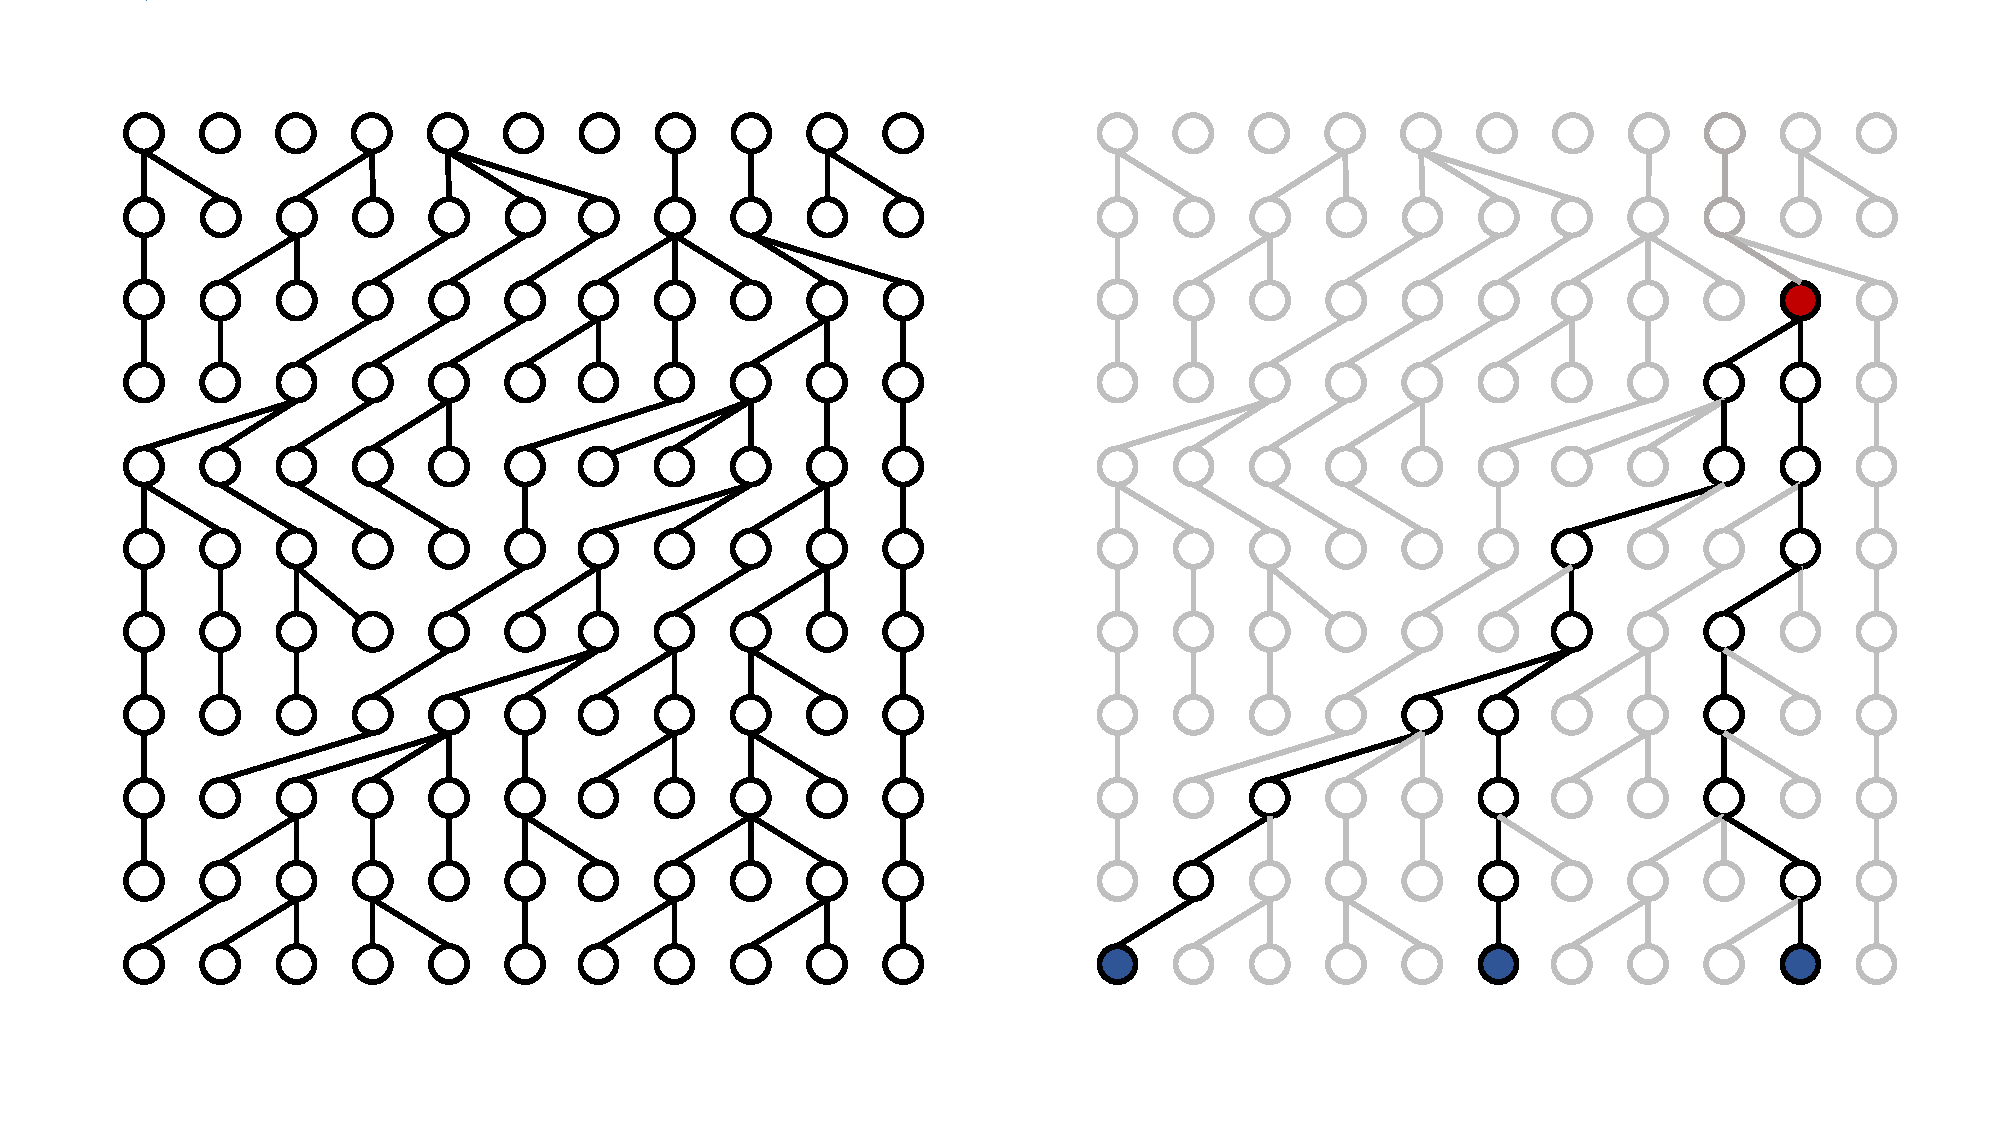
\includegraphics[width=\linewidth]{figures/wright_fisher.pdf}
    \caption{\textbf{Example of three lineages coalescing backwards in time in the Wright Fisher model.} Each individual chooses its ancestors from the set of ancestors with replacement until all the lineages coalesce into a single common ancestor. The three samples are colored blue and the common ancestor for the three samples red }
    \label{fig:coalescent}
\end{figure}

It is possible to derive the probability distribution of the time to the most recent common ancestor (TMRCA) under the Wright-Fisher model assuming a constant effective population size $N_e$. The TMRCA for a pair of samples is geometrically distributed and takes the form:
\begin{equation}
P(\tau_2 = t) = \left(1 - \frac{1}{N_e}\right)^{t-1} \frac{1}{N_e}
\end{equation}
where $\tau_2$ is the time to most recent common ancestor, and $N_e$ is the effective population size. The cumulative distribution function (cdf) of $\tau_2$ looks like:
\begin{equation}
P(\tau_2 \leq t) = 1 - \left(1 - \frac{1}{N_e}\right)^{t}
\end{equation}

Assuming a large and constant population size, $N_e \rightarrow \infty$ and setting $T_2 = \frac{\tau_2}{N_e}$ we can approximate the cdf as follows:
\begin{equation}
\begin{aligned}
    P(T_2 \leq t) &= P(\tau_2 \leq N_et) = P(\tau_2 \leq \lfloor N_et \rfloor) \\
    &= 1 - \left(1 - \frac{1}{N_e}\right)^{\lfloor N_et \rfloor} \\
    & \rightarrow 1 - e^{-t} \text{  as  } N_e \rightarrow \infty
\end{aligned}
\end{equation}

Note that the TMRCA takes the form of a standard exponential distribution. This is the coalescent model, introduced by Kingman in 1982 \cite{kingman1982coalescent, Kingman1982b, Kingman1982c}. As we will see the coalescent is a simplification of the Wright-Fisher model \cite{Wright1931, Fisher1930} for large populations which generalizes to various features in human genetics like mutations, recombinations and population structure. 

It is possible to generalize the coalescent to \(n\) lineages instead of a pair. Let us define $\xi(\tau)$ as the number of lineages remaining at time $\tau$ (in generations). Going backward in time with the initialization $\xi(0) = n$, $\xi(\tau)$ behaves as a Markov process. That is the distribution of $\xi(\tau + 1)$ only depends on the previous one, $\xi(\tau)$. We can define the transition probability of going from $i$ lineages to $j$ lineages in one generation as:
\begin{equation}
    p_{i,j} = P(\xi(\tau + 1) = j \mid \xi(\tau) = i)
\end{equation}

It can be shown under the standard coalescent model, setting $N_e \rightarrow \infty$ and ignoring second order terms, the transition matrix simplifies as follows:
\begin{equation}
\begin{aligned}
    &p_{i,i} \approx 1 -  \frac{\binom{i}{2}}{N_e} \\
    &p_{i,i-1} \approx \frac{\binom{i}{2}}{N_e} \\
    &p_{i,j} \approx 0 \text{  for any  } j < i - 1
\end{aligned}
\end{equation}

This implies the coalescent for \(n\) samples only allows one pair of lineages to coalesce per generation, making a binary ``coalescent'' tree. Additionally, the rate of coalescence depends on the number of lineages present at a given time. Let $T_j = \frac{\tau_j}{N_e}$ be the times when $j$ ancestors remain (scaled by the population size $N_e$) then according to the coalescent $T_j$ is independent of $T_i$ ($i \neq j$) and is distributed as follows:
\begin{equation}
    T_j \sim exp \left( \binom{j}{2} \right)  \text{,   } f_j(t) =  \binom{j}{2}e^{- \binom{j}{2}t}
\end{equation}

It is possible to generalize the above model for time-varying population sizes. Let us define the effective population size at time $t$ as $N_e(t)$. We can write the effective population size as a product of population size at $t=0$ and relative population size $\nu(t)$. Scaling the coalescence times based on population size at $t=0$, $N_e(0)$, the probability distribution when $j$ ancestors remain is given as follows:
\begin{equation}
    P(T_j > t \mid T_n + T_{n-1} + ... + T_{j+1} = s) = exp\left( - \binom{j}{2} \int_{s}^{s+t} \frac{1}{\nu(u)} du  \right)
\label{eq:coal_general}
\end{equation}

The above equation simplifies to the standard coalescent with constant population size if we set $\nu(t) = 1$. 

%% mention about inference of coalescene rates from a pair of lineages

\textbf{Coalescent with mutations:} To simulate mutations on the coalescent, we make an additional assumption called the infinite sites assumption. This assumption states that whenever a mutation occurs, it will always result in a new and unique mutated site, thereby disallowing any site from having more than one mutation. In humans, where the size of the genome is on the order of \(10^9\) bases and the mutation rate is on the order of \(10^{-8}\) per base per generation, it is realistic to assume that a mutation does not hit the same site more than once. We can model mutations as a homogeneous Poisson process on the coalescent. This means the total number of mutation events will follow a Poisson distribution with mean \(\mu t L\), where \(\mu\) is the mutation rate per base pair per generation, \(t\) is the time to the most recent common ancestor in generations, and \(L\) is the length of the genomic span being considered in base pairs. This is the generative model. During inference, where we already have information about mutations, we aim to reconstruct population characteristics backward in time.

\textbf{Coalescent with recombination:} In addition to modeling mutation, we also need to account for recombination to fully infer human population characteristics. We can modify the coalescent model to account for recombination as follows: Each pair of lineages can not only coalesce but also undergo recombination events, which split the ancestry of a single lineage into two parts. Going backward in time, at each generation, each segment of DNA can trace its ancestry independently, potentially to different ancestors. This process creates a branching structure where different segments of an individual's genome may trace back to different ancestors, creating a more complex ancestral structure than simple coalescence. This model is called the coalescent with recombination \cite{Hudson1983}. This graph structure was first introduced in \cite{Griffiths1997}, and is called the ancestral recombination graph (ARG). An illustrative example of an ARG is depicted in Figure \ref{fig:arg}. ARGs induce a sequence of trees along the genome (see Figure \ref{fig:arg}b). Genome-wide inference of ARGs is also loosely referred to as inferring genome-wide genealogies. In this thesis, we use the terms genealogies, tree sequences, and ARGs interchangeably, but a more descriptive difference can be found in \cite{wong2023general}.

%% change this to ARGs = tree sequences
\begin{figure}[h!]
    \centering
    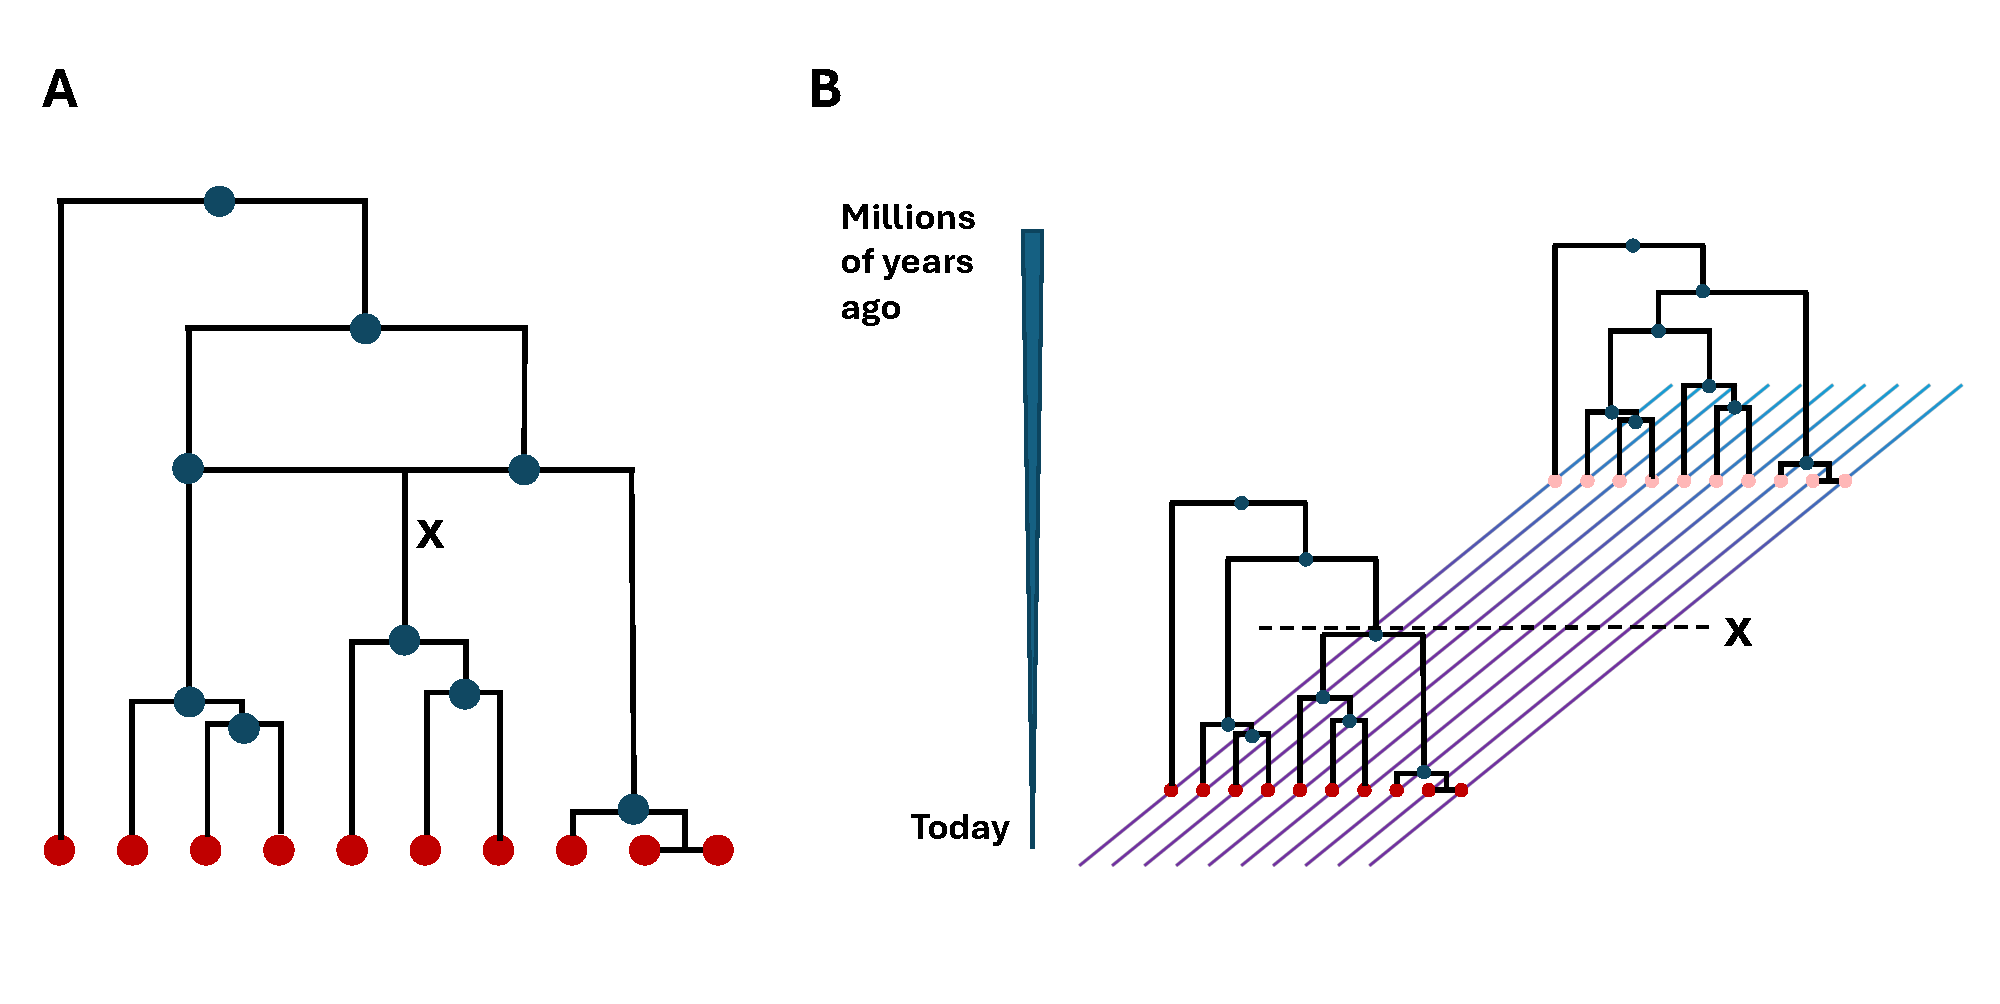
\includegraphics[width=\linewidth]{figures/coalescent_arg.pdf}
    \caption{\textbf{Example of an ancestral recombination graph (ARG) and the corresponding sequence of trees.} A. In the coalescent with recombination model the Lineages going backward in time can either coalesce or recombine, which means different portions of the genome have slightly different history. B. Corresponding sequence of trees representation of the ARG, \textbf{X} denotes the recombination position.}
    \label{fig:arg}
\end{figure}

The generality and simplicity of the coalescent limiting model enables extending it to account for many factors, including non-uniform recombination rates, time-varying population sizes and multiple samples. There is a suite of methods to infer these ARGs which rely on the coalescent theory. We will introduce some of these methods in Section \ref{sec:ch1-arg-inference}.

\textbf{Estimation of coalescence rates for a pair of lineages:} We can also perform inference under the coalescent. Let us simplify the coalescent for a pair of haplotypes and infer time-varying coalescence rates assuming piece-wise constant coalescence rates. We assume step-wise constant coalescence rates defined by fixed time intervals or epochs, labeled as $T_{1}$,  $T_{2}$, ... $T_{m}$. Let us say the coalescence rate is the parameter to be inferred and is given by $\gamma(e)$. The epoch index when the coalescence happens in the $l$-th tree is given by $e_l$ and  the coalescence time is denoted by $t_l$ ($T_{e_l} \leq t_l \leq T_{e_{l} + 1} $). Extending the coalescent from Equation \ref{eq:coal_general} for piece-wise constant coalescence rates, we can write the likelihood of the coalescence time as:
\begin{equation}
    P(t_l) = \gamma(e_l) e^{  -\gamma(e_l) (t_l - T_{e_l}) } \prod_{e=1}^{e_l} e ^{  -\gamma(e - 1) (T_{e} - T_{e-1}) } 
\end{equation}

For maximum likelihood estimation, we assume the $\mathbf{L}$ trees are independent, so we sum the log-likelihood across trees and estimate the coalescence rates by maximizing the following:
\begin{align}
    \log P(t_l) &= \log \gamma(e_l) - \gamma(e_l) (t_l - T_{e_l}) - \sum_{e=1}^{e_l} \gamma(e - 1) (T_{e} - T_{e-1}), \nonumber \\
    \log P(t) &= \sum_{l=1}^{\mathbf{L}} \left( \log \gamma(e_l) - \gamma(e_l) (t_l - T_{e_l}) - \sum_{e=1}^{e_l} \gamma(e - 1) (T_{e} - T_{e-1}) \right).
\end{align}

The MLE estimate for the coalescence rates are given by: 
\begin{equation}
    \hat{\gamma}(e) = \frac{n_e}{\sum_{l:e=e_l} (t_l - T_e) +  \sum_{l:e<e_l} (T_e - T_{e-1})}
\label{eq:gb_pairwise_gamma}
\end{equation}
where, $n_e$ is the number of trees which coalesce in the $e$-th epoch and is referred to as ``coalescence count'' and $\sum_{l:e=e_l} (t_l - T_e) +  \sum_{l:e<e_l} (T_e - T_{e-1})$ is the sum of branch length until the haplotype coalesces and is referred as the ``opportunity''. 

\subsection{Survey of methods to infer population structure and admixture history}
\label{sec:ch1-gb-survey}
Current methods to infer population structure can be classified into two main categories. The first set of approaches are model-based approaches, where the methods rely on a predefined generative model of how the population structure would impact the genetics and use this model to solve the reverse problem of inferring the population structure given the genetics. Popular model-based methods to identify population structure include Structure \cite{Pritchard2000}, Admixture \cite{Alexander2009}, and FineStructure \cite{Lawson2012}. The other category of methods are model-free approaches, which do not rely on modeling assumptions and are more exploratory in nature. Dimensionality reduction methods like Principal Component Analysis (PCA) are a popular example of such methods. The choice of which method to use depends on the type of genetic data being analyzed, computational resources, data sizes, and modeling assumptions.

Some of the earliest methods to understand population structure relied on quantifying genetic distances between individuals within and across predefined reference populations. One such measure, the ``fixation index'' also referred to as \(F_{st}\) \cite{Wright1951, Malecot1948}, measures the normalized allele frequency difference between two populations and within a population. Under several simplifying assumptions, including constant population sizes, the fixation index equals \(1 - T_0/T\), where \(T_0\) and \(T\) are the average coalescence times for individuals within the population and between two populations, respectively. The index is bounded from 0 to 1, where 0 refers to when the two populations are indistinguishable from each other, and 1 refers to when they are highly diverged. Since \(F_{st}\) measures genetic differences between populations due to genetic drift, population size plays a vital role in dictating how much drift is present. Smaller population sizes experience stronger drift, making methods that rely solely on \(F_{st}\) sensitive to assumptions about population sizes.

Early work to infer population structure also relied on analyzing variation in the Y-chromosome and mitochondrial DNA (mtDNA), as they have lost their ability to recombine \cite{Cann1987, tilford2001physical}. This allows for inferring a single genealogical tree that relates various populations, instead of an ARG or an average genealogical tree. In particular, the analysis of population structure using Y-chromosome or mitochondrial DNA involves considering prespecified ``haplogroups'', which are specific haplotypes thought to have arisen early in human history and are present in differing amounts in various human populations. By analyzing the number of specific haplogroups among populations, one can infer the coalescence times and topology of the genealogical tree explaining this pattern. Additionally, because Y-chromosomes are only inherited from the paternal lineage and mtDNA from the maternal lineage, this allows inference of population history that might be sex-biased. Although its importance in identifying sex-biased population structure persists even today, the number of haplogroups is limited, making it not always possible to discern subtle differences in populations by only looking at the Y-chromosome or mtDNA.

A popular model-based method to infer population structure is ``STRUCTURE'' \cite{Pritchard2000}, which clusters individuals into a fixed number of distinct populations based on their genotypic similarity. STRUCTURE assumes a similar generative model as latent Dirichlet allocation (LDA) in machine learning \cite{Blei2003}, which is used for topic modeling (though STRUCTURE predates LDA). The method works by partitioning the individuals into \(K\) populations, each characterized by allele frequency spectrum. It explicitly models the probability of observing the genotypes given the data and the assignment of the individual and proceeds with a Bayesian algorithm to infer the assignment of the individual and the corresponding allele frequencies that define the clusters. Several developments have improved the scalability of STRUCTURE, including methods like ADMIXTURE \cite{Alexander2009} and fastSTRUCTURE \cite{Raj2014}.

% cite eigenstrat
PCA is a model-free method to infer and visualize population structure in the data \cite{menozzi1978synthetic,Patterson2006, price2006principal}. It proceeds by eigen-decomposing the genotype matrix for all individuals and projecting the samples onto the top \(K\) eigenvectors. Due to eigen-decomposition, the top \(K\) eigenvectors maximize the amount of variance explained while being orthogonal to each other. It has been demonstrated that the top eigenvectors or principal components of the genotype matrix can capture the demographic history of samples without any specific modeling assumptions about the demography \cite{Patterson2006,novembre2008interpreting}. For example, the first two principal components (PCs) of a widely studied human genetic dataset, HGDP+1000 Genomes, clearly separate populations from sub-Saharan Africa from the rest of the samples. Furthermore, PC3 and PC4 start separating populations outside Africa. An accompanying plot which includes the principal components for the UK Biobank data is presented in Figure \ref{fig:pc_plot}. This plot is taken from \cite{bycroft2018uk}.

\begin{figure}[h!]
    \centering
    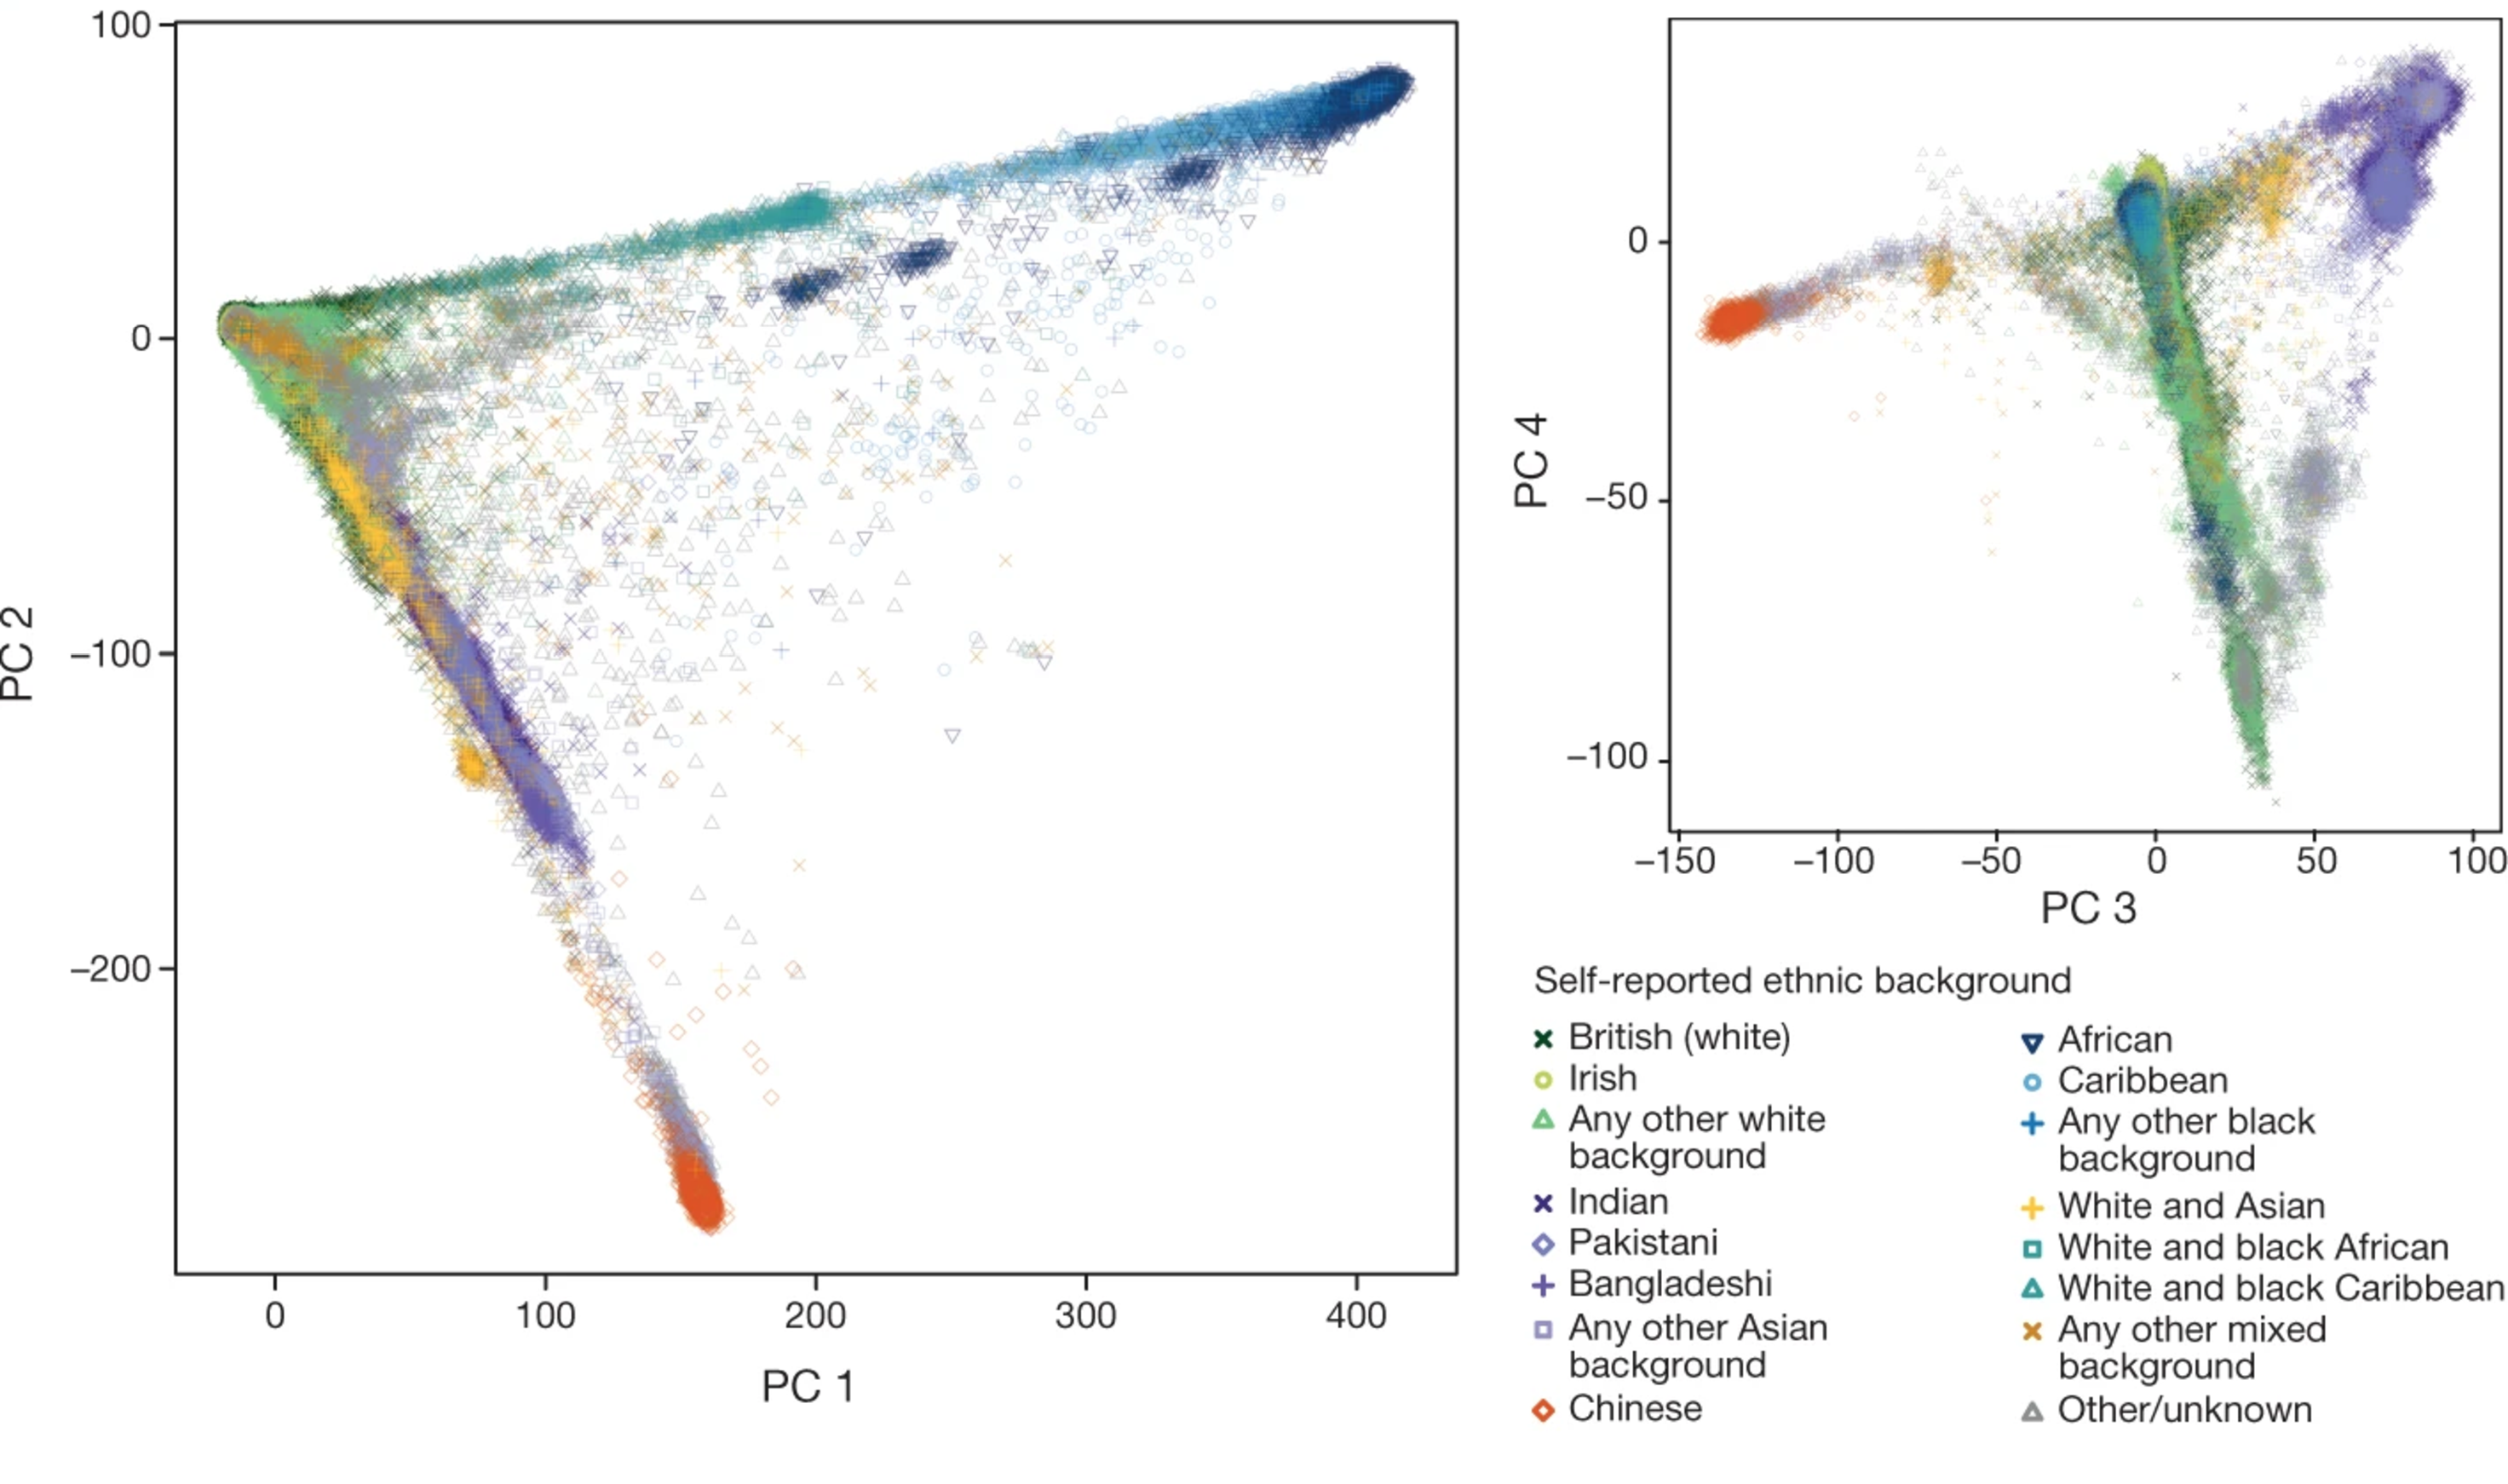
\includegraphics[width=\linewidth]{figures/thesis_pc_plot.pdf}
    \caption{\textbf{PCA visualization of $500,000$ individual genotypes from the UK Biobank.} PC1 and PC2 separate the African individuals from non-African individuals, whereas PC3 and PC4 separate individuals in Eurasia. The figure was taken from \cite{bycroft2018uk} (Creative Commons License).}
    \label{fig:pc_plot}
\end{figure}

% cite plos one paper nick patterson
Both STRUCTURE and PCA work well when the population structure is strong, making differences in allele frequencies or genotypes among individuals identifiable from noise \cite{Patterson2006}. There are a suite of methods to infer more subtle differences in populations, also referred to as fine-scale population structure. Identity-by-descent (IBD) methods use shared genetic segments between individuals to identify recent genetic relatedness and infer fine-scale population structure \cite{nait2020identity}. Other Methods like ChromoPainter and FineStructure \cite{Lawson2012} are model-based and use the Li and Stephens \cite{Li2003} algorithm to model an individual's haplotype as a mosaic of other individuals in a reference panel. Once the chromosome is painted, follow-up methods like FineStructure summarize the painting. The Li and Stephens algorithm is also used extensively to infer genealogies from sequencing data, as we will see in Section \ref{sec:ch1-arg-inference}.

Methods to identify population structure can also identify signatures of admixture in the data. For example, if there is recent admixture between two populations, the individuals who are admixed would have their STRUCTURE assignment as a mixture of two or more clusters, or would show a ``cline'' in the PCA, representing a continuum of ancestry between source groups. The American individuals in the HGDP+1000G dataset are admixed with varying admixture proportions from Native Americans, Europeans, and Africans, and this can be visualized in the PC plots in Figure \ref{fig:pc_plot}.

Other methods to infer admixture can characterize the admixture event by inferring an admixture date. Methods like Globetrotter \cite{hellenthal2014genetic}, TRACTS \cite{gravel2012population}, ALDER \cite{loh2013inferring}, and Rolloff \cite{moorjani2011history, patterson2012ancient} use haplotype information to infer admixture proportions, sources, and admixture times. The idea behind these methods is based on the observation that if admixture is recent, there will be long segments of DNA from each ancestry because there has been less time for recombination to mix the ancestries thoroughly. In a simple 2-way admixture, the length of the DNA segment from a particular ancestry is exponentially distributed with the rate proportional to the admixture time; this is called a co-ancestry curve. More formally, the probability of no recombination between two points a distance $g$ (in genetic distance units) apart since admixture is $e^{-g\lambda}$, where $\lambda$ is the admixture time. For a two-way admixture model with a single pulse of gene flow, the joint probability of ancestries at loci separated by a genetic distance $g$, conditional on recombination, is given by:
\begin{equation}
\begin{aligned}
    p_{AA}(g) &= \alpha ( e^{-g\lambda} + \alpha (1-e^{-g\lambda} )), \\
    p_{AB}(g) &= p_{BA}(g) = \alpha (1 - \alpha) (1 - e^{-g\lambda}), \\
    p_{BB}(g) &= (1-\alpha) ( e^{-g\lambda} + (1-\alpha) (1-e^{-g\lambda} ))
\end{aligned}
\end{equation}
where, $\alpha$ is the genome-wide proportion of ancestry `A' and $1-\alpha$ of ancestry `B'. In the case of multi-way admixture (more than two sources), the distribution becomes a mixture of exponential \cite{hellenthal2014genetic}. Therefore, using ChromoPainter to infer the painting of a target individual, methods like Globetrotter can accurately infer the admixture sources and admixture time. It is important to note that inferring admixture becomes challenging for old admixture events or admixture involving similar groups as recombination breaks up the long ancestry segments or ancestry segment inference becomes noisy when groups involved are very similar.

Once we identify the presence of an admixture event, various supervised learning methods can be employed to infer the local ancestry of a target. RFmix \cite{maples2013rfmix} uses support vector machines (SVMs) to classify regions of the sequence that belong to a particular reference population and infers the local ancestry quite accurately for recent admixtures between deeply diverged populations, such as the 3-way admixture in Americans. FLARE \cite{browning2023fast} is designed to scale efficiently to large sample sizes, while Mosaic \cite{salter2019fine} corrects for phasing errors during local ancestry inference and does not require prior knowledge of source groups, making it particularly useful for more complex scenarios.

%% can put after PCA, as its non-model based?
F-statistics are another suite of methods, first proposed by Nick Patterson \cite{reich2009reconstructing,reich2012reconstructing,patterson2012ancient,haak2015massive,durand2011testing}, which are useful for detecting population structure and admixture. These statistics, like the fixation index (\(F_{st}\)), rely on allele frequencies in different populations to infer genetic distances between individuals, the presence of admixture, or population splits in the dataset. There are three main kinds of f-statistics. The \(f_2\) statistic is simply the average squared allele frequency difference between two populations. Similar to \(F_{st}\), it measures the amount of genetic drift (and therefore genetic difference) between two populations. The \(f_3\) statistic is a three-population test measuring the amount of shared genetic drift between two populations from a common ancestor. The \(f_3\) statistic is also used as a test to detect admixture. The \(f_4\) statistic is a four-population test that measures how clade-like the four populations are. The \(f_2\), \(f_3\), and \(f_4\) statistics are defined as follows:
\begin{equation}
\begin{aligned}
    f_2(A, B) &= \frac{1}{L} \sum_{i=1}^{L} (p_{A,i} - p_{B,i})^2, \\
    f_3(A; B, C) &= \frac{1}{L} \sum_{i=1}^{L} (p_{A,i} - p_{B,i})(p_{A,i} - p_{C,i}), \\
    f_4(A, B; C, D) &= \frac{1}{L} \sum_{i=1}^{L} (p_{A,i} - p_{B,i})(p_{C,i} - p_{D,i})
\end{aligned}
\end{equation}
where, \( p_{X,i} \) is the allele frequency in population \( X \) at locus \( i \) and \( L \) is the number of loci considered. As \( f \)-statistics only use allele frequencies into account, they have become a widely used method to understand population structure, especially in ancient DNA studies where there is scarcity of high-coverage sequencing data but an abundance of low-coverage ancient samples. A more detailed explanation of \( f \)-statistics and their geometric interpretation can be found in \cite{peter2022geometric}.
% PCA-F stats paper.

\subsection{Large-scale inference of genome-wide genealogies}
\label{sec:ch1-arg-inference}
Many model-based methods to detect population structure and admixture rely on coalescent theory to model the likelihood of the observed genotype given the population sizes or admixtures. It is reasonable to question if we can infer the ARGs directly from the genetic variation data. Assuming the validity of assumptions under the coalescent, inferring the ARG directly would make understanding the evolutionary forces responsible for observed genetic variation much easier, as under the coalescent model the evolutionary forces impact the genetic variation through the ARGs (see Figure \ref{fig:ghostbuster_intro}).

\begin{figure}[h!]
    \centering
    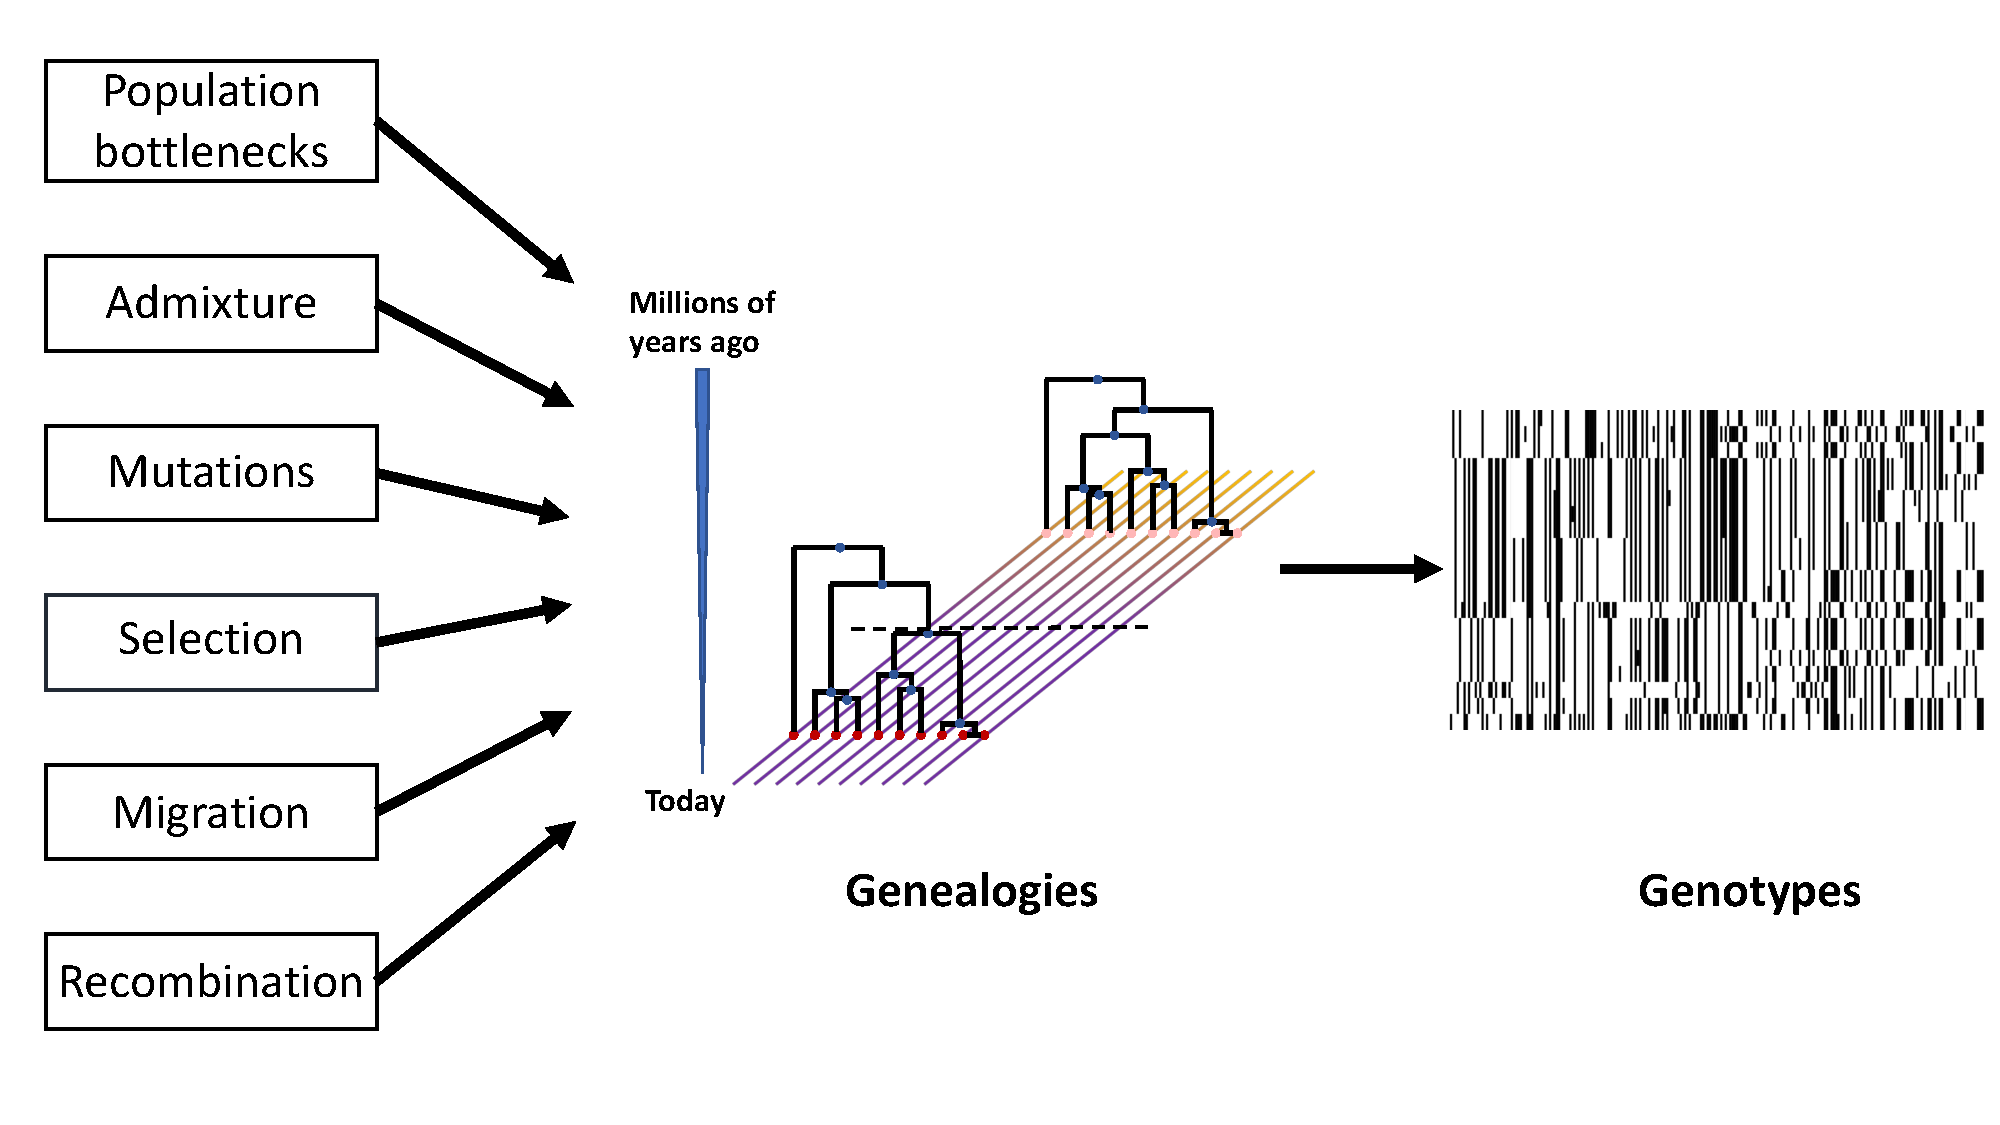
\includegraphics[width=\linewidth]{figures/thesis_ghostbuster_intro.pdf}
    \caption{\textbf{Evolutionary forces impact genotypes through genealogies.} Evolutionary forces like mutations, recombination, population bottlenecks, admixture, migration and selection affect the observed genotypes through the unobserved genealogies}
    \label{fig:ghostbuster_intro}
\end{figure}

Inferring Ancestral Recombination Graphs (ARGs) directly from genetic variation data is challenging because each recombination event splits the genealogical tree into two trees. The fact that mutation rates and recombination rates in humans (and many other species) are roughly similar means that, on average, there is only one mutation per branch on the tree, making it difficult to infer the genealogy. However, ARG inference methods leverage the fact that recombinations are unevenly distributed along the genome and still result in correlated adjacent trees. Over the past decade, new statistical methods have been developed to utilize these insights for ARG inference. 

ARG-weaver \cite{rasmussen2014genome} is one of the earliest scalable genealogy inference methods. ARG-weaver uses a Markovian approximation to the coalescent with recombination, the Sequentially Markovian Coalescent (SMC) \cite{mcvean2005approximating}, to constrain the space of possible ARGs. The SMC model reduces the search space of possible ARGs and makes it Markovian by ignoring coalescent events between lineages that do not share overlapping ancestral material. It essentially moves along the chromosome and updates the coalescent tree instead of the full ancestral recombination graph whenever a recombination occurs. ARG-weaver simplifies the inference of Ancestral Recombination Graphs (ARGs) by discretizing time, which further reduces the space of possible ARGs. It employs a Gibbs sampling approach, where a sample is threaded into the ARG based on the conditional probability of the rest of the ARG. Despite these approximations, ARG-weaver is limited in its scalability and can handle at most a few hundred samples.
% https://www.nature.com/articles/hdy201338
% McVean and Cardin (2005) 
% https://web.archive.org/web/20220517024716id_/https://www.biorxiv.org/content/biorxiv/early/2021/11/27/2021.11.15.468686.full.pdf

Tsinfer \cite{Kelleher2019} and tsdate \cite{wohns2022unified} are recent algorithms for ARG inference that are able to scale to hundreds of thousands of samples. Tsinfer uses a variation of the Li and Stephens algorithm to infer the tree sequence. It first estimates various possibilities of ancestral haplotypes at a given site and then uses the Li and Stephens copying process to paint the younger ancestors using older ancestors, thereby generating an ARG structure around the variant. Tsdate uses the topologies inferred using tsinfer to date the coalescence events using a conditional coalescent prior, conditioning on the number of descendants of each node on a local tree. Tsinfer and tsdate also demonstrated that storing genotype information in the tree sequence format saves a significant amount of disk space, leveraging the tree structure to save the variants instead of treating all variants independently.

Relate \cite{speidel2019method}, like tsinfer and tsdate, uses a variation of the Li and Stephens algorithm to infer genealogies and can scale to thousands of samples. It proceeds by using the Li and Stephens algorithm to calculate pairwise distances between samples at a given site, followed by hierarchical clustering to build a tree that best represents the observed variation around this site. Once the local trees are inferred and heuristically matched with adjacent trees, Relate estimates the coalescence times using an MCMC routine under the coalescent prior, conditioning on the tree topology. Relate also supports an iterative method to jointly estimate the population sizes along with estimating the coalescence times, making it more flexible for use in human datasets.

ARG-Needle \cite{zhang2023biobank} is another recent algorithm that is able to scale to hundreds of thousands of samples. Like ARGweaver, it threads a sample into the genealogy one at a time, but uses heuristics to speed up the process. It essentially proceeds as follows: for a new sample to be threaded, it detects \(K\) closely related samples around the variant, uses ASMC \cite{palamara2018high} to infer the coalescence times with those \(K\) possible samples, and then uses the sample corresponding to the minimum coalescence time to thread the new sample into the ARG. This process is repeated until all samples are threaded into the genealogy. Apart from genealogy inference, ARG-Needle also demonstrated the promise of using genealogies for phenotype prediction and association testing.

Singer \cite{deng2024robust} is a Bayesian method for ARG inference that scales to hundreds of samples. Like ARGweaver and ARG-Needle, Singer uses threading to infer the genealogies in a Bayesian way. Specifically, Singer employs a two-step threading algorithm where the first step samples the possible branch to thread and the second step samples the coalescence time for this threading. This is done under an MCMC routine, which enables the sampling of not only coalescence times but also tree topologies.

Overall, there has been recent development in accurate and scalable inference of genome-wide genealogies from genetic variation data. A recent evaluation of the performance of some of these ARG inference methods under some accuracy metrics can be found in \cite{brandt2022evaluation}. This opens a new suite of directions to understand the evolutionary forces responsible for our genetic variation using these genealogies. In the next section, we survey some novel methods that rely on genealogies and help us understand our human past more accurately.

\subsection{Genome-wide genealogies to understand evolutionary history}

By inferring genome-wide genealogies, we hope to be one step closer to understanding evolutionary history, as the evolutionary history has impacted genetic variation through these genealogies. Let us explore the various evolutionary forces we can infer once we know the genealogies.

\textbf{Inferring population sizes using genealogies:} Under the coalescent, the population sizes are defined as the reciprocal of the coalescent rates between individuals in the same population. Therefore, given the genealogy, it is straightforward to infer the population sizes. A common approach to infer these time-varying population sizes is to discretize the time into several epochs and count the number of coalescence events between individuals in each epoch, divided by the opportunity for the coalescence event to happen, that is, the sum of branch lengths in the epoch. In a simplistic case, this can be done for all pairs of individuals in the population, which results in an unbiased estimate of the population size.

\textbf{Inferring population structure using genealogies:} Following the argument for inferring population sizes, one can also infer cross-population coalescence rates, that is, the chance of coalescence between two individuals from different populations. These rates are a common way to identify population structure or migration \cite{schiffels2014inferring}, as populations with higher cross-coalescence rates would be more similar to each other either due to a recent population split or recent migration between the two populations.

\textbf{Inferring presence of admixture using genealogies:} A simple way to identify recent admixture in a genealogy is by looking at genealogical nearest neighbors. If there is a recent admixture event, different regions of the genome would have different affinities to reference populations. A straightforward method to infer regions of the genome where a target individual is closer to one population than another is to look at its first coalescence event with the reference panel. A population description of the sister individuals at the tree would roughly indicate which population the target individual most closely relates to in that section of the genome. This is also how admixture inference methods like ChromoPainter work. A more careful analysis is needed if there are multiple admixture events or if the admixture event is old and can not be summarized by just the first coalescence event. Our method, GhostBuster (discussed in Chapters 2-3), addresses this problem. 

\textbf{Inferring positive selection:} Relate \cite{speidel2024high} devised a simple statistic to detect the presence of positive selection in the data. Specifically, the statistic compares the speed of spread of a certain lineage relative to other lineages in the tree. Relate's selection test uses results from the standard coalescent to model the joint distribution of the number of descendants given \(k\) lineages. Relate's selection test produced controlled false positive rates while outperforming other selection inference methods, such as singleton density scores \cite{field2016detection}, which did not leverage the genealogy to infer selection. A similar test was devised in ASMC \cite{palamara2018high}, where they considered pairwise genealogies and regions of significantly lower TMRCA to detect positive selection. Additionally, CLUES \cite{stern2019approximate} and CLUES2 \cite{vaughn2024fast} use inferred genealogical information in an importance sampling scheme to directly estimate the likelihood of alleles under selection.

Among other applications, twigstats \cite{speidel2024high}, used inferred genealogies to more accurately estimate f-statistics. By effectively truncating trees and focusing only on mutations in the recent part of the tree, twigstats improved f-statistics standard errors to detect fine-scale structure. Another approach, introduced glike \cite{fan2023likelihood}, involves estimating the likelihood of the observed genealogy given the demographic parameters, thereby accurately estimating parameters like population sizes, admixtures, and migrations from the observed genealogies. This method surpasses techniques that only use genetic data for inference. ARG-based methods also have their limitations. Firstly, most methods rely on the inferred ARG to be an accurate estimate of the true underlying genealogy. Second, ARG-based methods are not necessarily computationally faster than methods which directly operate on genotype data. Third, accurate estimation of ARGs currently requires high-quality genetic data, which may not always be available. However, despite these limitations, ARG-based methods provide powerful insights into population history and evolutionary processes that are difficult to achieve with other approaches. A comprehensive review comparing different ARG inference methods and discussing their application in understanding human history can be found in \cite{brandt2024promise, nielsen2024inference}.

\subsection{Motivation for GhostBuster}

% Paragraph 1 is Problem formulation (often combined with next paragraph)
% Paragraph 2 is Previous work on the problem (often combined with next paragraph)
% Paragraph 3 is Challenges that have yet to be solved
% Paragraph 4 is New approach to these challenges
% Paragraph 5 (optional) is Overview of results/interpretation (often
% combined with previous paragraph)

% Population demographic factors, such as population structure and migrations, have shaped the genetics of present-day samples, consequently affecting phenotypes. The advent of large-scale genomic datasets and theoretically grounded methods to analyze this data have enabled better understanding of this human population history. Previous methods for understanding human population history typically rely on deriving some summary statistics from genetic data to infer the presence of admixture and population structure. However, identifying subtle changes in population history directly from the genetic data is challenging, especially when there is minimal external evidence or when source groups remain unsampled. These are called ghost events or ghost populations. Large-scale inference of genome-wide genealogies has enabled a more direct examination of the demographic factors influencing genetics, resulting in more powerful inferences.

% In this thesis we propose a method, called GhostBuster, which utilizes genealogies to understand past demographic factors like migrations and admixtures more accurately and in a more interpretable manner. Through simulations and real-data examples, we demonstrate that GhostBuster can successfully recover signatures of both ancient and recent admixtures, accurately identifying source groups, admixture times, and local ancestry of target individuals. Notably, we infer a back-to-Africa migration that contributed up to 8\% Eurasian ancestry to sub-Saharan Africans between 5,000 and 15,000 years ago. Additionally, we identify and characterize a deep admixture event in Africa involving ghost populations, which split around 300,000 years ago and mixed within the last 50,000 years to form the present-day sub-Saharan African populations.

% Demographic factors - population structure, migration, admixture
% Cite previous methods
% Examples of events which are not well characterized
% Methods like globetrotter can resolve recent history 1000-2000 years ago
% ancient DNA has extended it to several 1000 years
% archaics 50k years, but adna is limited and difficult to get older in time
% making inferences about deep human past difficult


% Mention GB is a mixture model, clusters trees


Population movements and mixtures have been a constant feature of human history across various time scales. Notable examples include the Out of Africa migration, Neanderthal and Denisovan introgression over 40,000 years ago, multiple admixtures in Holocene Europe, and recent migrations and multi-way admixtures in the Americas within the last few hundred years (see Figure \ref{fig:gb-intro}a-c). Despite this, the genetic legacy of some events remains elusive due to the limited resolution of statistical methods and the scarcity of ancient DNA samples (see Figure \ref{fig:gb-intro}d).

Many previous methods for deciphering admixtures have relied on detecting long segments of DNA corresponding to recent admixture events. These methods often use admixture LD to date admixtures, which have proven effective for identifying events within the last few thousand years. However, as recombination events shorten these segments, the statistical power of these methods diminishes, making it challenging to infer older admixtures \cite{hellenthal2014genetic, loh2013inferring, moorjani2011history, patterson2012ancient}. Another widely used approach involves sequencing or genotyping ancient DNA samples, providing direct evidence of the genetic makeup of our ancestors. Ancient DNA studies, employing methods such as PCA \cite{Patterson2006}, STRUCTURE \cite{Pritchard2000}, and f-statistics \cite{reich2009reconstructing,reich2012reconstructing,patterson2012ancient,haak2015massive,durand2011testing}, have significantly extended our understanding of human history up to approximately 10,000 years ago—beyond the temporal reach of LD-based methods. However, the deeper human past remains difficult to uncover due to the scarcity of ancient DNA samples from earlier periods, which are challenging to preserve over such long timescales. While the limited number of archaic DNA samples has offered some insights, they remain insufficient to fully reconstruct the complex genetic history of early human populations.

Furthermore, previous methods typically rely on deriving summary statistics from genetic data to infer the presence of admixture and population structure. Identifying subtle changes in population history directly from genetic data is particularly challenging when there is minimal evidence or when source groups remain unsampled. The large-scale inference of genome-wide genealogies provides a more direct approach to examining the demographic factors influencing genetic variation. By modeling these demographic changes, genealogies offer a more interpretable and detailed view of human history, allowing researchers to trace population dynamics with greater accuracy and uncover previously hidden aspects of our ancestral past.

In this thesis, we introduce a novel method called GhostBuster, which leverages coalescent theory and inferred genealogies to analyze past mixture events with greater statistical power and interpretability. GhostBuster is a mixture model that clusters the genealogical history of a target individual based on its coalescence rates with a set of reference populations. This approach not only characterizes mixture events but also decomposes the local ancestry of target individuals. Unlike traditional methods, GhostBuster does not require sampled source populations to identify admixture events, making it capable of detecting ghost admixtures. Through simulations and real-data examples, we demonstrate that GhostBuster can successfully recover signatures of both ancient and recent admixtures, accurately identifying source groups, admixture times, and the local ancestry of target individuals.

We apply GhostBuster to both modern and ancient samples from sub-Saharan Africa, a region where ancient DNA is particularly scarce due to environmental conditions that hinder DNA preservation. Our analysis uncovered two significant events that occurred in Africa. First, we identified a Holocene-era back-to-Africa migration that introduced detectable levels of Eurasian ancestry into all sub-Saharan African populations we analyzed. This event, which occurred between the last millennium and approximately $10{,}000$ years ago, provides a plausible explanation for the presence of small amounts of Neanderthal ancestry in modern Africans. Leveraging inferred local ancestry, we detected differential enrichment for specific trimer mutations, including TCC to TTC substitutions, which have been previously linked to West Eurasian populations \cite{harris2015evidence}. Further characterization of this event using coalescence rate affinities with various ancient populations revealed that the Eurasian ancestry in Africans may trace back to early European farmers from Anatolia, suggesting a potential spread of farming practices from Europe to the Middle East and North Africa, eventually reaching sub-Saharan Africa. The second event represents a more ancient admixture between two African population groups, one of which is closely related to the out-of-Africa population that gave rise to present-day Eurasians. Our findings suggest that these populations diverged at least $300{,}000$ years ago and subsequently admixed around or after the major out-of-Africa migration. This admixture is associated with differences in population sizes and PRDM9 hotspot activity between the two groups. Furthermore, we observed distinct affinities of these ancient populations with other archaic humans, such as Neanderthals and Denisovans, from that era. Finally, our analysis revealed that the two ancient populations exhibit differing levels of polygenic score (PGS) portability when genome-wide association studies (GWAS) are conducted in European cohort, highlighting the importance of ancestry decomposition in understanding genotypic variation affecting phenotypes.

% advantage of looking at genealogy







\begin{figure}[h!]
    \centering
    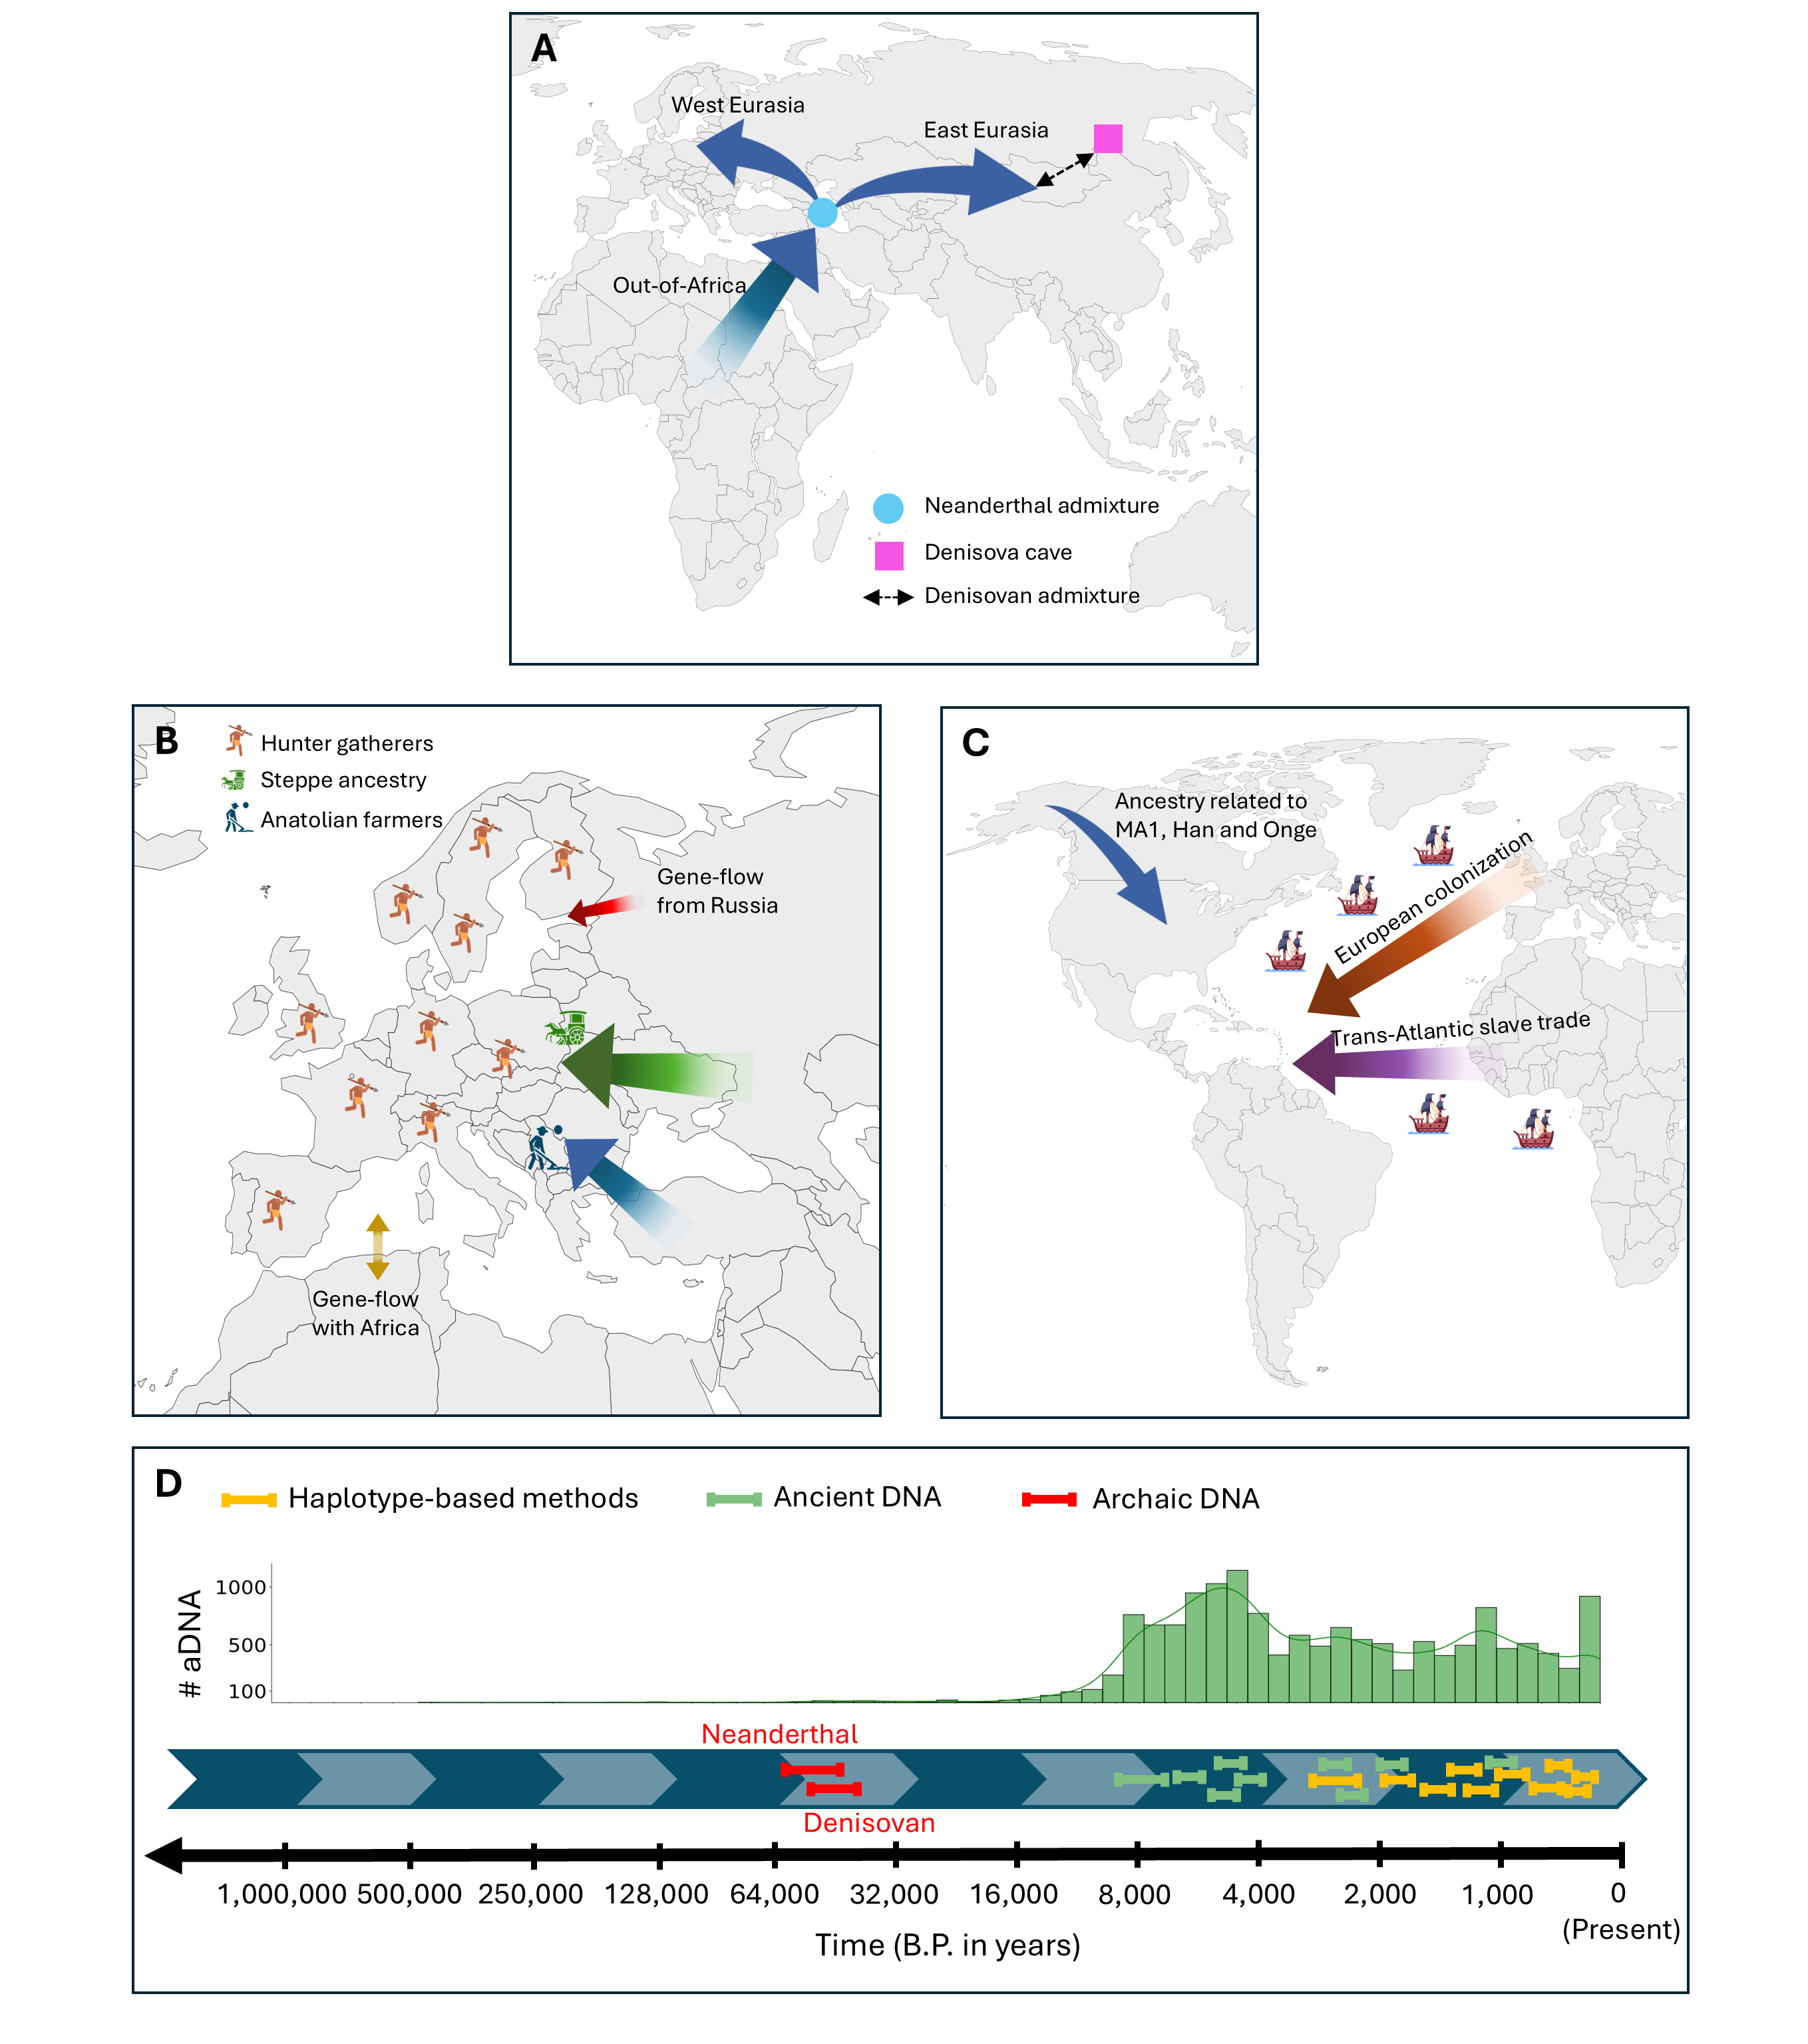
\includegraphics[width=\textwidth]{figures/thesis_gb_migration_example_v2.png}
    \captionsetup{width=\textwidth+3cm}
    \caption{
    \footnotesize
    \textbf{Some examples of migration and admixture events in human history.} A. Archaeological and genetic evidence suggests modern humans originated in Africa and migrated out between 50,000 and 100,000 years ago \cite{darwin1874descent, lopez2015human}. They interbred with Neanderthals, contributing up to 3\% of non-African DNA. After leaving Africa, the population split into west and east Eurasian groups, creating genetic differences between Europeans and Asians. East Eurasians also admixed with Denisovans, though the timing and location are debated \cite{jacobs2019multiple, reich2010genetic}.
    %
    B. Europe has experienced significant migrations, starting with Anatolian farmers 7,000-9,000 years ago, followed by Steppe pastoralists around 5,000 years ago, which heavily influenced present-day European ancestry. There is also evidence of recent gene flow from North African groups into southern Europeans, such as Italians and Spanish, and ancient Siberian-related ancestry in northeastern Europeans like Finns and Russians \cite{haak2015massive, salter2019fine}.
    %
    C. The peopling of America likely began during the last glacial period, which created a land bridge to Eurasia \cite{severinghaus1999abrupt}, ending around 15,000 years ago. Ancient DNA in America shows genetic links to ancient Siberians (MA1), Han Chinese, and the Onge tribe \cite{skoglund2016genomic}. Present-day American genetics are influenced by historical events like colonization and the trans-Atlantic slave trade, resulting in admixture from Native American, African, and European sources \cite{smith2004high, price2009sensitive}.
    %
    D. Previously identified human admixtures were determined using various methods, including haplotype-based approaches \cite{hellenthal2014genetic, loh2013inferring, moorjani2011history, patterson2012ancient}, ancient DNA, and archaic DNA analyses. The histogram shows the ages of ancient DNA samples sequenced to date, sourced from the Allen Ancient DNA Resource \cite{mallick2024allen}.
    The illustrations were downloaded from Flaticon.
    }
    \label{fig:gb-intro}
\end{figure}

%% add timeline to the figure

\clearpage

\section{Understanding complex traits through genetic data}

An important line of work in statistical genetics focuses on understanding how the patterns of genetic variation in present-day individuals affect phenotypes. The first disease gene was mapped in 1983, identifying a polymorphism on chromosome 4 responsible for Huntington's disease \cite{Gusella1983}. This study involved analyzing pedigrees with fewer than 100 samples to pinpoint the genetic cause of Huntington's disease. Huntington's disease is an example of a monogenic disorder, where a single alteration in the genome explains the entire genetic basis of the disease. With the growing size of genetic datasets, we now know that most complex traits and diseases in humans are not monogenic but polygenic, where hundreds or thousands of small alterations in the genome explain the genetic basis of a trait. Finding these small polygenic effects spread across the genome requires examining genetic variation data genome-wide in a larger number of samples.

The Wellcome Trust Case Control Consortium (WTCCC) \cite{WTCCC2007} was one of the first efforts to perform a large-scale genetic association study. It genotyped 17,000 individuals, comprising 2,000 cases and 3,000 common controls across seven common diseases (type 1 diabetes, type 2 diabetes, coronary heart disease, hypertension, bipolar disorder, rheumatoid arthritis, and Crohn's disease). The WTCCC performed a genome-wide association study to look at polymorphisms in the genome that correlate more than usual with the case-control status and found 90 new variants across all the diseases analyzed, confirming the presence of 28 previously established variants. Since then, Genome-wide association studies have become a cornerstone in current-day quantitative genetics to understand how genetic variation affects phenotypes.


\subsection{Basic definitions}

The heritability of a trait, roughly speaking, is the proportion of total trait variance explained by genetic variation. It measures how important genetics are in predicting a given trait, where a heritability of 1 means genetics explain all the variance in the trait between individuals, and a heritability of 0 means genetics do not explain any variance in the trait. It is important to note that heritability for a trait depends on the quality of phenotypic measurements and the environment itself. Heritability should not be confused with the variance associated with the direct biological mechanisms affecting a trait. In many complex traits, the path from genes to traits is complex and indiscernible \cite{Neale2017}. A more detailed understanding of heritability, its implications, and common misunderstandings can be found in \cite{Visscher2008,Gusev2021}.
% http://www.nealelab.is/blog/2017/9/13/heritability-101-what-is-heritability#:~:text=For%20example%2C%20the%20heritability%20of,all%20the%20relevant%20genetic%20effects).
% http://gusevlab.org/projects/hsq/

Linkage disequilibrium (LD) refers to the correlation patterns in genetic variation data due to the fact that variants close to each other are transmitted together more frequently than variants further away from each other. LD is further exacerbated because most recombination in humans happens at recombination hotspots, creating distinct LD patterns along the genome. LD can be both a boon and a bane in analyzing human variation data. It is a boon because common variants can capture the signal from nearby unobserved causal variants, thus improving the power of predicting the phenotype using the variation data. However, it is a bane because the same LD makes it challenging to distinguish causal variants from associated variants, as tightly correlated variants obscure the identification of the true causal variant.

Two major challenges in performing genome-wide association studies (GWAS) are the presence of population structure and relatedness in the data, both of which can confound genetic signals and inflate test statistics. We have already discussed population structure in the context of population genetics in Section \ref{sec:ch1-gb-basic-defination}. In quantitative genetics, population structure can lead to allele frequency differences between cases and controls, resulting in spurious associations between genotypes and traits — a phenomenon known as population stratification. Relatedness between samples is another significant confounder in association testing and is typically estimated through the genetic relatedness matrix (GRM). The (GRM) is computed as \(\frac{XX^T}{M}\), where \(X\) is an \(N \times M\) genotype matrix, \(N\) is the sample size, and \(M\) is the number of variants. The GRM plays a crucial role in linear mixed model (LMM) methods, which are widely used in GWAS to account for these confounders. We will discuss LMM methods in more detail in Section \ref{sec:ch1-lmm}.


\subsection{Genome-wide association studies: usage and applications}
\label{sec:ch1-qd-gwas-applications}

After it became clear that many human traits are polygenic in nature, an unbiased genome-wide scan for variants associated with these traits was warranted. Following the first large-scale genome-wide association study published by the Wellcome Trust Case Control Consortium (WTCCC) in 2007, a huge wave of large-scale population-wide studies aimed at understanding the genetic architectures of various complex traits ensued. Today, 17 years after WTCCC, GWAS has become a standard protocol for understanding the genetic basis of most complex traits. With sequencing and phenotyping efforts from pharmaceutical industries, academia, and independent nation-wide ``biobanks'', GWASs have been performed on thousands of human traits, using millions of individuals, and have identified hundreds of thousands of genetic associations \cite{GWASCatalog}. %GWAS catalog

GWAS has become a vital element in drug discovery, with two-thirds of the new drugs approved by the FDA in 2021 supported by human genetic evidence \cite{rusina2023genetic,ochoa2022human,abdellaoui202315}. Some examples include Finerenone, an NR3C2 antagonist approved for the treatment of chronic kidney disease \cite{teumer2019genome,bakris2020effect}. Baricitinib, identified through GWAS studies for COVID-19 severity, was shown to reduce the COVID-19 mortality rate by approximately 20\% \cite{favalli2020baricitinib,horowitz2022genome}. It is important to note that GWASs are not enough to support drug target discovery on their own. Further downstream analysis, such as replication, expression QTL studies in relevant tissues and cell types, and understanding off-target effects, are necessary and are part of the GWAS pipeline to obtain suitable drug targets.
% https://www.nature.com/articles/s41467-019-11576-0

Apart from identifying genetic associations with traits, GWAS is also utilized to build polygenic scores for a trait or disease susceptibility. Polygenic scores, or PGS, use the estimated effects for a trait to build a predictor of the genetic likelihood of a trait. PGS have found clinical potential for personalized medicine and treatment, with current utility for various genetic disorders including cardiovascular diseases \cite{torkamani2018personal}. GWAS has also enabled the identification of genetic similarity between traits and diseases, helping to identify biological pathways for gene functions \cite{solovieff2013pleiotropy}. On a more general level, GWAS hits have also helped us understand the evolution of certain human traits, where selection mechanisms like directional, stabilizing, and pleiotropic are among the most likely explanations of how trait-associated variants spread forward in time \cite{simons2018population}. Additionally, GWAS has been useful in causal inference studies, as a genetic instrument in Mendelian randomization, helping to identify disease-causing traits \cite{davey2014mendelian, pingault2018using}. An overview of the GWAS pipeline and its application can be found in Figure \ref{fig:qd-intro} and following reviews \cite{visscher201710, abdellaoui202315}.

\begin{figure}[h!]
    \centering
    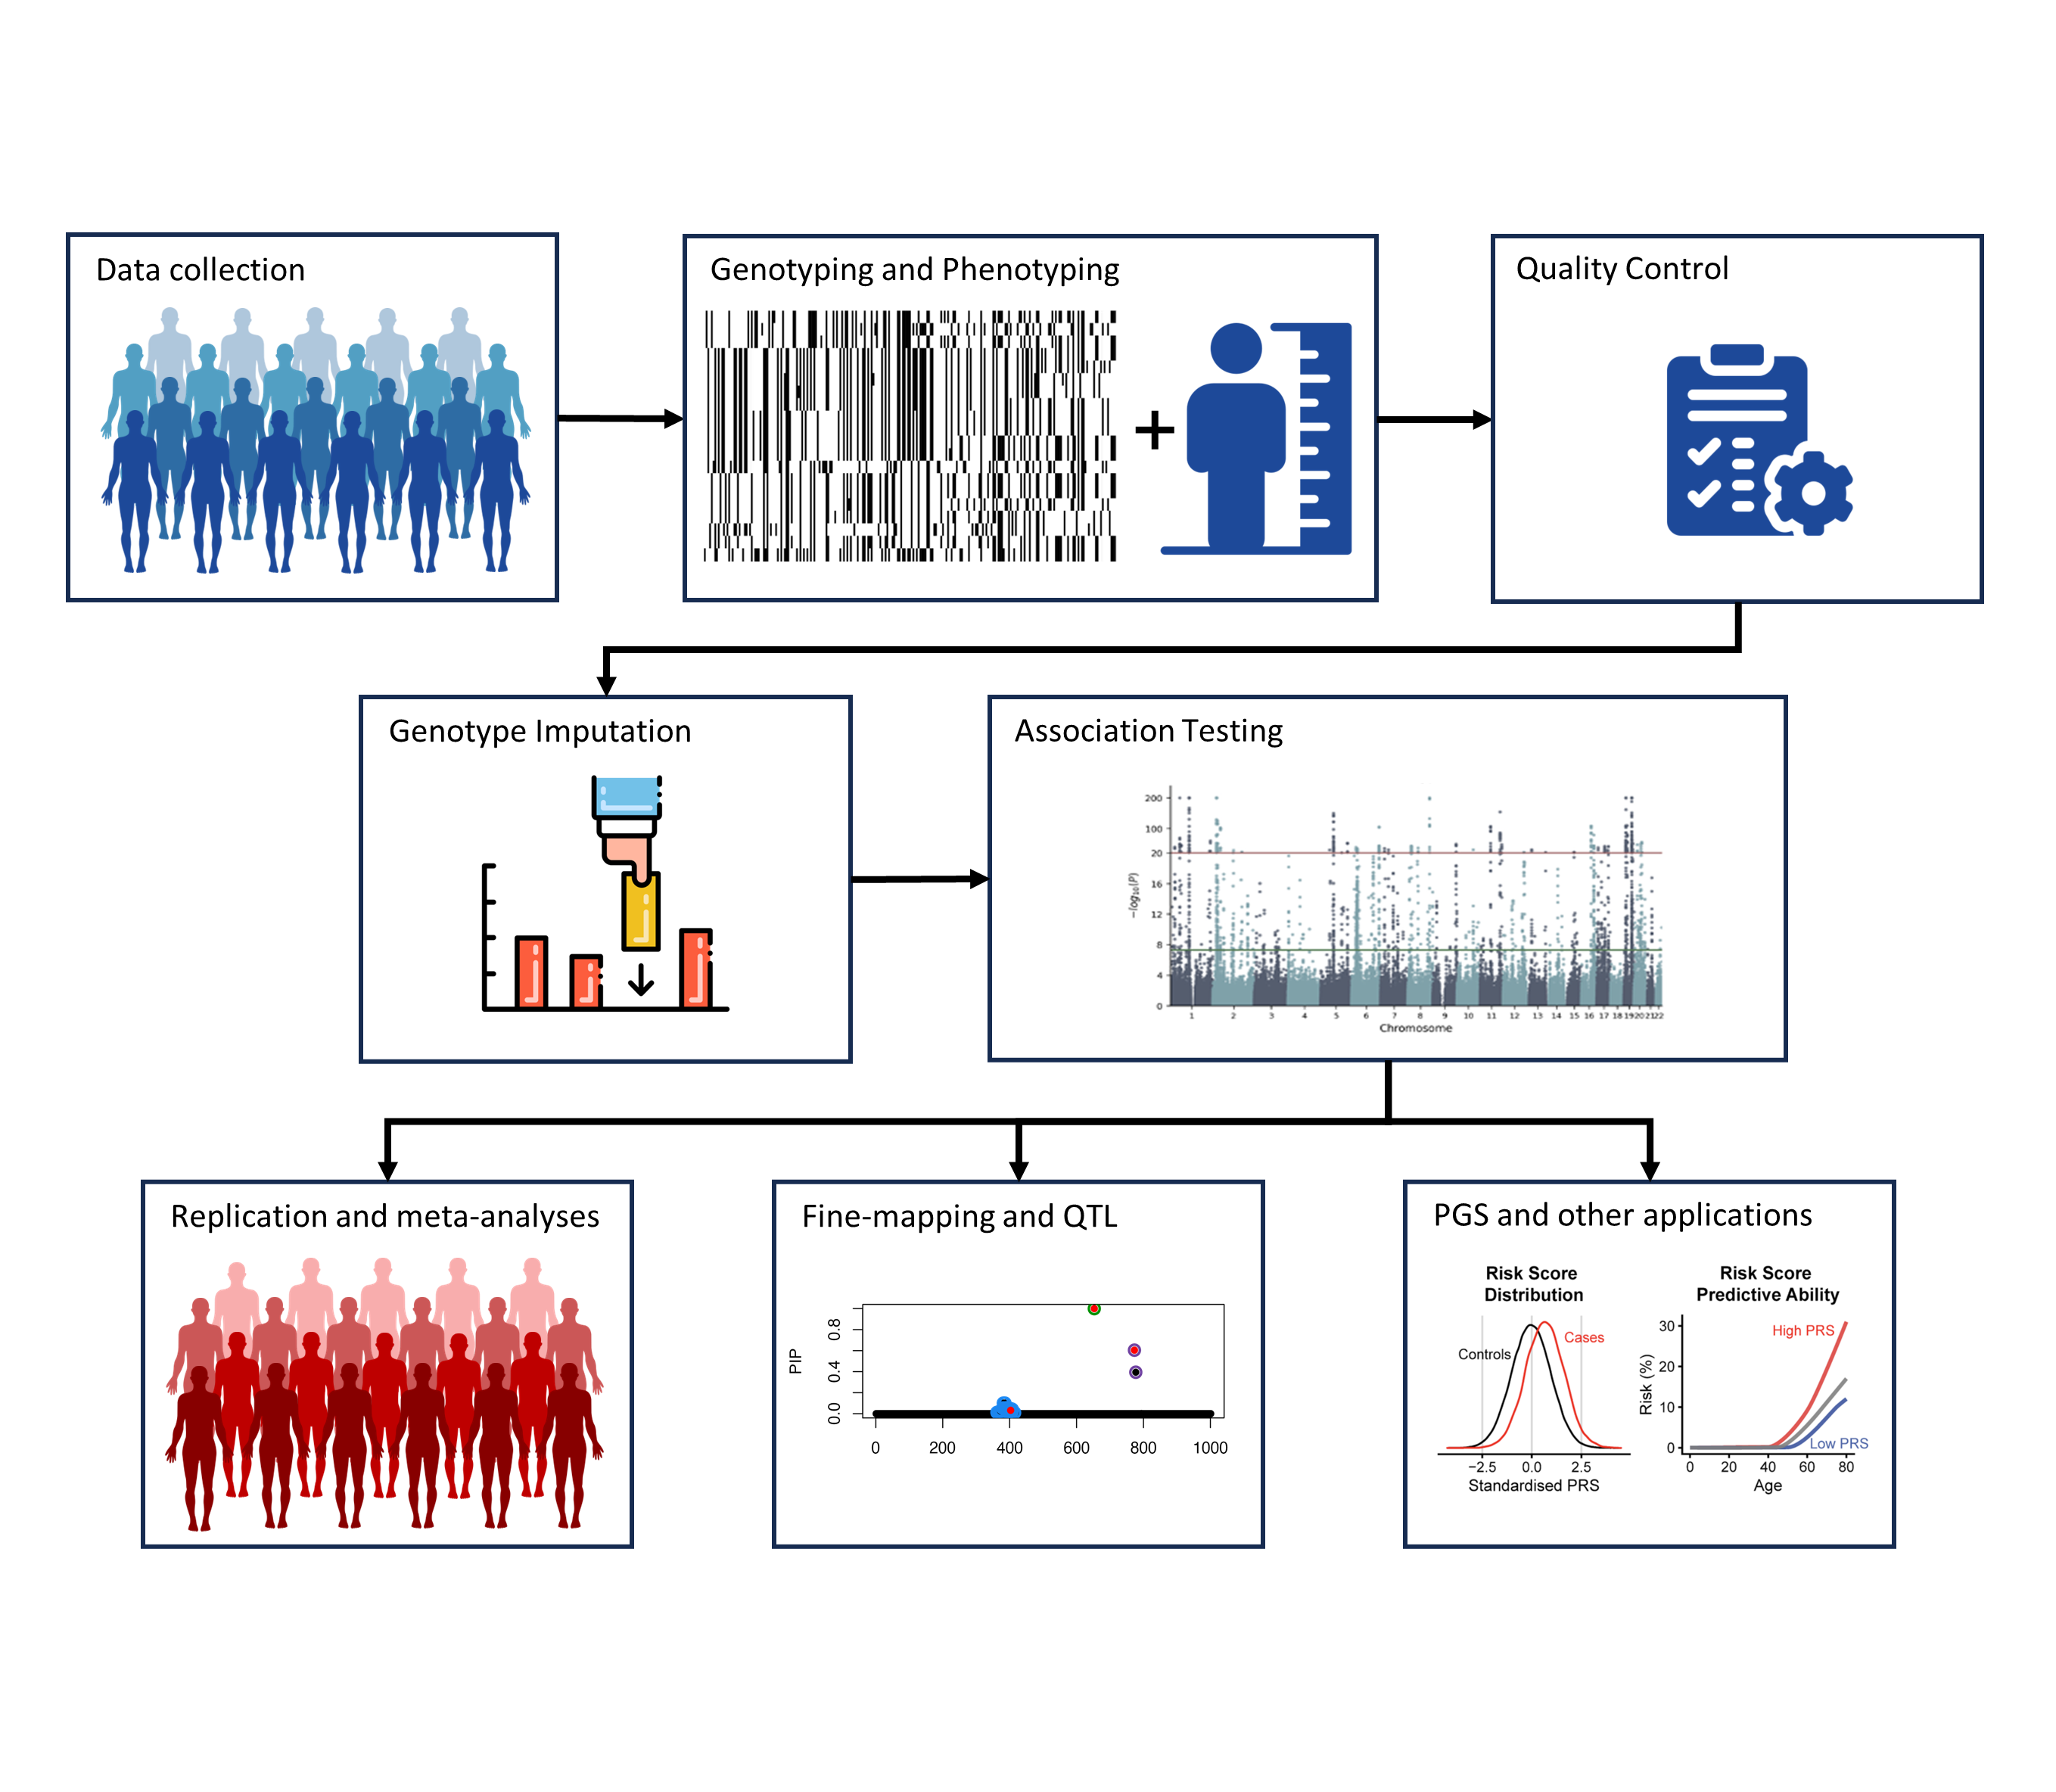
\includegraphics[width=\textwidth]{figures/thesis_qd_gwas_pipeline.png}
    \caption{
    \textbf{Overview of a typical GWAS pipeline.} The GWAS pipeline typically begins with genotyping and phenotyping a large cohort of individuals, including both cases and controls for disease traits. Genotyping can be conducted using either low-cost SNP arrays or whole-genome sequencing. Quality control steps are crucial and involve filtering variants and samples based on various criteria (see Section \ref{sec:ch5-data} for detailed quality control procedures). If genotyping was performed instead of whole-genome sequencing, genotype imputation follows as the next step. Subsequently, genome-wide association testing is conducted for each variant and phenotype of interest to generate p-values and effect estimates, indicating the association between each variant and the phenotype. The resulting GWAS summary statistics have several downstream applications. These include replication and meta-analyses to increase statistical power, fine-mapping and functional analyses to identify causal variants among the associated variants, and the calculation of polygenic scores. This pipeline structure was adapted from \cite{uffelmann2021genome}, with the fine-mapping figure from \cite{Wang} and the polygenic scores figure from \cite{wand2021improving}.}
    \label{fig:qd-intro}
\end{figure}

\subsection{Theoretical framework to perform GWAS}
\label{sec:ch1-lmm}
There are two main categories of methods to perform genome-wide association studies. The first set of methods involves fitting a linear model to estimate the effect of a variant on the phenotype, taking into account various covariates. The linear models fit the following model:
\begin{equation}
    y = x_{test}\beta_{test} + \alpha C + \epsilon. \label{linear}
\end{equation}

In the above, \(y\) is an \(N \times 1\) vector of mean-centered and standardized phenotype values, \(x_{test}\) is an \(N \times 1\) vector of mean-centered and standardized bi-allelic variant values (that is, the original \(\tilde{x}_{test}\) takes values in \(\{0,1,2\}^N\) for diploid samples), \(C\) is an \(N \times C\) matrix of covariates of interest, such as principal components, age, and sex, and \(\epsilon\) is Gaussian noise.

Linear models fit the model in Equation \ref{linear} using a simple OLS estimate for linear regression or an iterative scheme for logistic regression. Test statistics are calculated from standard closed-form solutions for the standard error of the estimates. However, simple linear models fail to correct for the presence of population structure and cryptic relatedness in the data, making the resulting test statistic estimates inflated. Therefore, methods that rely on linear models require working with a subset of unrelated and homogeneous individuals to ensure the false positive rates are not too high. This, in turn, reduces the sample size and power to detect genetic associations in the dataset.

The second class of methods are Linear mixed models or LMMs. LMMs are an extension of linear models that facilitate the analysis of non-independent data. They are commonly adopted in the analysis of genomic data involving population structure or cryptic relatedness. LMMs handle non-independence by modeling random effects that capture variability within different subpopulations or phenotypic correlation across close relatives. In an LMM for genome-wide association analysis, the phenotype of interest is often modeled as a combination of fixed effects, which include the effects of the test variant and covariates, and random effects, which include genetic effects and environmental effects:
\begin{equation}
    y = x_{test}\beta_{test} + \alpha C + g + \epsilon \label{lmm}.
\end{equation}

Similar to the linear model above, $y$ is an $N \times 1$ vector of mean-centered and standardized phenotype values, $x_{test}$ is an $N \times 1$ vector of mean-centered and standardized bi-allelic variant values, $C$ is an $N \times C$ matrix of covariates.
%
We are mainly interested in inferring the fixed effect of a particular variant, $\beta_{test}$, given the random genetic effects, which help capture the effects of population structure and relatedness.
%
We model the genetic and environmental effects using
\begin{align}
    g &= \beta_{GRM} X_{GRM} \nonumber \\
    \epsilon &\sim  \mathcal{N}(0, \sigma^2_e) \label{lmm-1},
\end{align}
where $X_{GRM}$ is an $N \times M_{GRM}$ standardized genotype matrix and $\sigma^2_e$ is the environmental variance for a given phenotype.
%
For simplicity, the environmental random effect is assumed to be independent and identically distributed (i.i.d.) from a normal distribution, and the random genetic effect is modeled as a weighted sum of standardized genotypes. The random genetic effect $g$ can also be thought of as a sample from $\mathcal{N}(0, \sigma^2_g K)$, where $\sigma^2_g$ is the genetic variance for a given phenotype and $K = \frac{1}{M}X_{GRM}X_{GRM}^T$ is the genetic relatedness matrix.




\textbf{Leave-one-chromosome-out: }
%
It has been observed that in order to avoid reducing the power of association, the matrix $X_{GRM}$ should not contain the test variant $x_{test}$, as well as any other variants in linkage disequilibrium (LD) with $x_{test}$.
%
This problem has been referred to as ``proximal contamination'' \cite{listgarten2012improved}.
%
Fitting an LMM with genetic effects from variants not in LD with the testing variant, however, would require re-training the model to infer genetic effects for every tested variant, which would cause major computational overheads.
%
\cite{yang2014advantages} proposed a simple solution to this problem, referred to as the leave-one-chromosome-out (LOCO) scheme, where the $X_{GRM}$ is constructed using all variants except those on the same chromosome as the test variant.
%
For example, assuming $22$ autosomal chromosomes and a test variant on chromosome $7$, $X_{GRM}$ is built to contain all variants from chromosome $1$-$6$ and $6$-$22$.
%
This approach, which requires training a separate model for each chromosome, allows circumventing proximal contamination while increasing association power, and has been widely adopted by recent LMM association algorithms \cite{loh2015efficient,loh2018mixed,jiang2019resource}.
%
% Previous methods train 22 models (one per leave-one-chromosome) in parallel to estimate the effect estimates $\beta_{GRM}$ for each LOCO model and use them to calculate the test-statistics by choosing the correct LOCO model. 

\textbf{Calculation of the test statistic: }
%
To infer the fixed effect $\beta_{test}$ in Equation \ref{lmm}, one can marginalize the random effects $\beta_{GRM}X_{GRM}$ and $\epsilon$ to get the marginalized log-likelihood:
\begin{align}
    y \mid x_{test}, \beta_{test}, \sigma_e^2, \sigma_g^2 &\sim \mathcal{N}(x_{test}\beta_{test}, \frac{\sigma_g^2}{M} X_{GRM}X_{GRM}^T + \sigma_e^2 I_N) \nonumber \\
    \log P(y \mid x_{test}, \beta_{test}, \sigma_e^2, \sigma_g^2) &\propto -\frac{1}{2} (y-x_{test}\beta_{test})^TV^{-1}(y-x_{test}\beta_{test}) -\frac{1}{2} \lvert \log(V) \rvert,
\label{eq:full_like}
\end{align}
where $\sigma_g^2$ and $\sigma_e^2$ are genetic and environmental variance components as described above, and $V$ is a covariance matrix, defined as $V = \frac{\sigma_g^2}{M} X_{GRM}X_{GRM}^T + \sigma_e^2 I_N$.
%

The maximum likelihood estimate (MLE) for $\beta_{test}$ is obtained by setting $\frac{\partial \log P(y \mid x_{test}, \beta_{test})}{\partial \beta_{test}} = 0$; the variance of the estimate is obtained using the inverse Fisher information $ -\mathbf{E}\left[\frac{\partial ^2 \log P(y \mid x_{test}, \beta_{test})}{\partial \beta_{test}^2} \mid \hat{\beta}_{test}\right]^{-1}$ and takes the form:
\begin{align}
    \hat{\beta}_{test} &= (x_{test}^T V^{-1} x_{test})^{-1}(x_{test}^T V^{-1} y) \nonumber \\
    var(\hat{\beta}_{test}) &=(x_{test}^T V^{-1} x_{test})^{-1} \label{lmm-inf}.
\end{align}

%
The variance components, $\sigma_g^2$ and $\sigma_e^2$, are estimated using restricted likelihood maximization (REML) \cite{loh2015efficient} or moment-based methods \cite{wu2018scalable,pazokitoroudi2020efficient} rather than standard maximum likelihood estimation.
%
In this work, we estimate the variance components $\hat{\sigma}_g^2$ and $\hat{\sigma}_e^2$ using the RHE-MC algorithm \cite{wu2018scalable,pazokitoroudi2020efficient}, a highly scalable moment-based approach that was recently extended to allow processing multiple traits in parallel \cite{zhu2024ARGRHE}.
%
We then estimate the covariance matrix using $\hat{V} = \frac{\hat{\sigma}_g^2}{M} X_{GRM}X_{GRM}^T + \hat{\sigma}_e^2 I_N$, and the effects using
\begin{align}
    \hat{\beta}_{test} &= (x_{test}^T \hat{V}^{-1} x_{test})^{-1}(x_{test}^T \hat{V}^{-1} y), \nonumber \\
    var(\hat{\beta}_{test}) &= (x_{test}^T \hat{V}^{-1} x_{test})^{-1} \label{lmm-inf2}.
\end{align}

%
Using the asymptotic property of the MLE, 
\begin{equation}
   \frac{\hat{\beta}_{test} - \beta_{test}}{\sqrt{var(\hat{\beta}_{test})}} \sim \mathcal{N}(0, 1) 
\end{equation}

%
To test the null hypothesis $\beta_{test} = 0$, we therefore substitute the MLE estimate and the variance of the estimate from Equation \ref{lmm-inf2}, and square both sides to get:
\begin{equation}
   \frac{(x_{test}^T \hat{V}^{-1} y)^2}{x_{test}^T \hat{V}^{-1} x_{test}} \sim \chi^2_1 \label{lmm-chi2-rep}.
\end{equation}


There are two common modeling assumptions for the distribution of genetic effects along the genome, leading to different LMM foundations - Infinitesimal and non-infinitesimal models. 

%
\textbf{Infinitesimal model: }
%
The infinitesimal model places a normal prior on the effect estimates $\beta_{GRM}$ from Equation \ref{lmm-1}, and assumes the total genetic effect explained by all the genetic markers to be $\sigma_g^2$:
\begin{equation}
    \beta_{GRM} \sim \mathcal{N}(0, \sigma_g^2 I_M/M)
\end{equation}

%
As the prior and likelihood are conjugate, we can infer the posterior distribution $P(\beta_{GRM} \mid X_{GRM}, y)$:
\begin{equation}
    \begin{split}
        P(\beta_{GRM} \mid X_{GRM}, y) = \mathcal{N}\Bigg( &\left( \frac{I_M M}{\sigma_g^2} + \frac{X_{GRM}^T X_{GRM}}{\sigma_e^2} \right) ^{-1} \frac{X_{GRM}^T y}{\sigma_e^2}, \\
        &\left( \frac{I_M M}{\sigma_g^2} + \frac{X_{GRM}^T X_{GRM}}{\sigma_e^2} \right) ^{-1} \Bigg) \label{lmm-inf3}
    \end{split}
\end{equation}

%
The maximum-a-posteriori (MAP) estimate of $\beta_{GRM}$ in Equation \ref{lmm-inf3}, also referred to as the best linear unbiased predictor (BLUP), can be written as:
\begin{equation}
    \hat{\beta}_{GRM} = \left( \frac{I_M M}{\sigma_g^2} + \frac{X_{GRM}^T X_{GRM}}{\sigma_e^2} \right) ^{-1} \frac{X_{GRM}^T y}{\sigma_e^2} 
\end{equation}

%
The residual phenotype, formed by regressing out the effect of other variants on the phenotype, is given by $\tilde{y} = y - X_{GRM} \hat{\beta}_{GRM}$ and simplifies to
\begin{equation}
    \tilde{y} = y - X_{GRM} \hat{\beta}_{GRM} = \sigma_e^2 V^{-1} y
    \label{blup_lmm_link}
\end{equation}

%
This provides a link between the BLUP and test statistics for $x_{test}$ in Equation \ref{lmm-chi2-rep}, which is exploited to compute test statistics for non-infinitesimal models.
%
Under the infinitesimal model, the test statistic can be rewritten as:
\begin{equation}
    \frac{(x_{test}^T \tilde{y}/\sigma_e^2)^2}{x_{test}^T \hat{V}^{-1} x_{test}} \sim \chi^2_1
    \label{blup_lmm-rep}
\end{equation}

%
% Write about the frequentist approach, prior on $\beta_{GRM}$ and chi-square test statistics derivation
% Derive the BLUP estimates and show how the numerator in chi-square is related to phenotype residual
%
\textbf{Non-infinitesimal model: }
%
It is often the case that a large fraction of variants are not linked to the phenotype, so the above model can be improved by adopting a more appropriate prior, such as a spike-and-slab prior, or a mixture-of-Gaussian prior.
%
The spike-and-slab prior can be modeled as follows:
\begin{equation}
P(\beta_{GRM}) \sim p_0 \mathcal{N} (0, \sigma_g^2/Mp_0) + (1-p_0) \delta(0),
\end{equation}
where $\delta(0)$ is the Dirac-delta function at $0$.
%
A mixture-of-Gaussian prior replaces the Dirac-delta function using a low-variance normally distributed component, and can be written as:
\begin{equation}
P(\beta_{GRM}) \sim p_0 \mathcal{N} (0, \sigma_{g,1}^2/M) + (1-p_0) \mathcal{N} (0, \sigma_{g,2}^2/M).
\end{equation}

%

%
Equation \ref{blup_lmm-rep} can still be used to compute test statistics, by replacing $\tilde{y}$ with the phenotype residuals calculated using BLUP under the non-infinitesimal model.
%
Note that it is often not possible to obtain a closed-form solution for the BLUP under an non-infinitesimal model, but can be approximated through MCMC or variational inference algorithms.

\subsection{Survey of methods to perform GWAS}

Plink \cite{purcell2007plink} is one of the most widely used linear model-based GWAS algorithms. Its subsequent versions \cite{chang2015second} improve its scalability by implementing vectorized operations over phenotypes, working with the disk-space efficient pgen format, and supporting sparse matrix multiplication \cite{rivas2024efficient}. Despite its efficiency, Plink does not implement a linear mixed model to correct for population structure and relatedness, and therefore is only used with unrelated homogeneous subsets of the data.

EMMA \cite{kang2008efficient} is among the earliest methods to implement a linear mixed model for association testing in human datasets. It optimized the fixed effects by maximizing the full likelihood in Equation \ref{eq:full_like} relying on spectral decomposition. The overall algorithm was still cubic in sample size and required constructing the \(N \times N\) kinship matrix. EMMAX, or EMMA expedited \cite{kang2010variance}, was a follow-up to EMMA which improved its scalability by more than two orders of magnitude. Instead of recomputing the variance parameters for each variant separately, EMMAX observed that a single variant does not have a huge effect on the variance components and therefore estimated it once and reused it for association testing.

Fast-LMM \cite{lippert2011fast} used the spectral decomposition of the kinship matrix and its low-rank representation to speed up association testing further compared to EMMAX. Fast-LMM-Select \cite{listgarten2013fast} followed as a subsequent method, which subsets the markers for kinship calculation based on their predictability for the trait using a linear model. It was later shown that this strategy of reducing the number of markers in kinship calculation leads to inflation in the test statistics, as background polygenic effects are not fully captured \cite{yang2014advantages}.

BOLT-LMM \cite{loh2015efficient,loh2018mixed} was one of the first methods to scale linearly with the number of markers and sub-quadratically with the number of samples. The overall complexity of BOLT-LMM is \(O(MN^{1.5})\). BOLT-LMM achieved this by using conjugate gradient techniques for matrix inversions (thus never explicitly computing the kinship matrix), an efficient grid search algorithm for estimating variance parameters, and a variational inference routine to predict the polygenic effects. Furthermore, BOLT-LMM's variational inference routine imposed a mixture of Gaussian priors on the effect estimates, allowing it to model the non-infinitesimal genetic architecture, which led to improved statistical power in GWAS.

The assumption of Gaussianity about the test statistic distribution is often violated in binary traits, especially when the ratio of cases to controls is imbalanced or when testing with a rare variant. SAIGE \cite{zhou2018efficiently} implements saddle point approximation (SPA) \cite{kuonen1999miscellanea,dey2017fast} to correct the test statistics and ensure calibration in binary traits. SAIGE also employs conjugate gradient tricks similar to BOLT-LMM, which speeds up the calculation of test statistics while avoiding explicit computation of the kinship matrix.

FastGWA \cite{jiang2019resource} and FastGWA-GLMM \cite{jiang2021generalized} are among the fastest methods to perform linear mixed model association testing for quantitative and binary traits. FastGWA-GLMM is the generalized mixed model extension of FastGWA, aimed at analyzing binary traits. These methods approximate the GRM as a sparse matrix, thresholding it to only keep close relatives. The sparse GRM is generated once and used for all subsequent analyses, making matrix multiplications in test statistics calculation extremely fast. However, approximating the kinship with a sparse matrix loses some statistical power compared to methods that use the dense matrix.

REGENIE \cite{mbatchou2021computationally} is a recent method for association testing that uses block-wise ridge regression to estimate the polygenic effect and then vectorized test statistics calculation routines, allowing for the analysis of multiple phenotypes at scale. REGENIE also implements an approximate version of Firth logistic regression and saddle point approximation to correct test statistics for binary traits. REGENIE scales linearly with sample size and number of markers, making it approximately two orders of magnitude faster than BOLT-LMM in the analysis of 50 quantitative traits in the UK Biobank. However, it still does not match BOLT-LMM's statistical power, as it does not account for the non-infinitesimal genetic architecture.

A table comparing modern GWAS methods can be found in table \ref{tab:gwas_methods}. 


\begin{sidewaystable}[h]
    \centering
        \begin{tabular}{|>{\centering\arraybackslash}m{0.1\linewidth}|>{\centering\arraybackslash}m{0.2\linewidth}|>{\centering\arraybackslash}m{0.1\linewidth}|>{\centering\arraybackslash}m{0.11\linewidth}|>{\centering\arraybackslash}m{0.11\linewidth}|
        >{\centering\arraybackslash}m{0.11\linewidth}|>{\centering\arraybackslash}m{0.11\linewidth}|} \hline 
             GWAS Method &  Main innovation & Scalability & Uses non-infinitesimal prior  & Multi-trait vectorization & Binary trait correction & Corrects population structure \& relatedness \\ \hline 
             Plink v2 & Implements a very fast linear model, uses efficient data storage and access & $\mathcal{O}(MN)$ & \xmark & \checkmark & \xmark & \xmark \\ \hline 
             BOLT-LMM & Implements a linear mixed model, uses variational inference to fit a mixture of normal prior on the effects  & $\mathcal{O}(MN^{1.5})$ & \checkmark & \xmark & \xmark & \checkmark \\ \hline 
             SAIGE v2 & Implements a logistic mixed model, uses sparse GRM and SPA to correct for binary traits & $\mathcal{O}(MN)$ & \xmark & \xmark & \checkmark & \checkmark \\ \hline 
             REGENIE & Implements block-wise ridge regression with SPA and Firth logistic regression to correct for binary traits & $\mathcal{O}(MN)$ & \xmark & \checkmark & \checkmark & \checkmark \\ \hline 
             FastGWA & Implements linear and logistic mixed model, uses sparse GRMs for quick test statistics calculation & $\mathcal{O}(MN)$ & \xmark & \xmark & \checkmark & \checkmark \\ \hline
        \end{tabular}
    \caption{\textbf{Comparison of methods to perform GWAS.} We compare five most popular GWAS softwares namely, Plink \cite{purcell2007plink}, BOLT-LMM\cite{loh2015efficient,loh2018mixed}, SAIGE\cite{zhou2018efficiently}, REGENIE\cite{mbatchou2021computationally} and FastGWA\cite{jiang2019resource, jiang2021generalized} comparing their overall scalability, ability to model non-infinitesimal genetic architecture for higher statistical power, multi-trait vectorization for better scalability, support for binary traits and ability to control FPR in presence of population structure and relatedness.}
    \label{tab:gwas_methods}
\end{sidewaystable}

\subsection{Motivation for Quickdraws}
As we saw in Section \ref{sec:ch1-qd-gwas-applications}, genome-wide association studies (GWAS) are a key step in modern analyses of complex traits and diseases.
%
These association studies are being enabled by the rapid growth of modern biobanks \cite{bycroft2018uk,nagai2017overview,ramirez2022all,wojcik2019genetic,chen2011china,kurki2023finngen}, which contain vast amounts of genomic, phenotypic, and environmental information for increasingly diverse groups \cite{zhou2022global}.
%
The scale of these data sets, however, creates several computational obstacles, which have led to significant advances in statistical methodology and the development of highly scalable linear-mixed-model GWAS algorithms \cite{yu2006unified,kang2008efficient,kang2010variance,zhang2010mixed,zhou2012genome,lippert2011fast,segura2012efficient,listgarten2012improved,listgarten2013fast,loh2015efficient,loh2018mixed,jiang2019resource}.
%
Among these, the BOLT-LMM algorithm \cite{loh2015efficient,loh2018mixed} achieves state-of-the-art association power by adopting a Bayesian mixture prior to model non-infinitesimal trait architectures, but is computationally intensive, particularly when applied to multiple traits, and has limited applicability to binary traits.
%
More recent methods, including SAIGE \cite{zhou2018efficiently}, FastGWA \cite{jiang2019resource,jiang2021generalized}, and REGENIE \cite{mbatchou2021computationally}, are highly scalable and may be used for the analysis of both quantitative and binary traits.
%
These algorithms have enabled performing GWAS for millions of genomic variants and individuals \cite{yengo2022saturated} across thousands of traits and diseases \cite{wang2021rare}, but rely on modeling approximations, such as the use of block-wise ridge regression
 or sparse genetic relationship matrices, that may reduce statistical power.
%
As a result, current GWAS algorithms are either highly scalable and cost effective or highly powered to detect association, but not both.

%
In this thesis we describe a method, called Quickdraws, that uses machine learning strategies to simultaneously achieve state-of-the-art association power and computational efficiency, while being applicable to both quantitative and binary traits.
%
%
Quickdraws uses a Bayesian regression model with a spike-and-slab prior on variant effects, which is efficiently trained by leveraging recent advances in stochastic variational inference, transfer learning, and graphics processing units (GPUs) matrix operations.
%
We use simulations to show that, applied to the analysis of quantitative traits, Quickdraws matches the association power of BOLT-LMM, the most powerful method, while requiring orders of magnitude less computation. 
%
For binary traits, Quickdraws achieves higher statistical power compared to existing methods such as SAIGE, REGENIE, and FastGWA, equivalent to analyzing up to $13.4\%$ more samples, while having a comparable computational speed.
%
We apply Quickdraws and other methods to test $13.3$ million variants for $50$ continuous blood-related traits and $50$ disease traits in up to ${\sim}405k$ individuals from the UK Biobank data set \cite{bycroft2018uk}.
%
For quantitative traits, Quickdraws identifies $4.97\%$ more independent associations than REGENIE and $22.71\%$ more than FastGWA; for disease traits, it detects $3.25\%$ more associations than REGENIE and $7.07\%$ more than FastGWA.
%
These associations result in similar gains in the number of replicated signals in Biobank Japan \cite{nagai2017overview} and Finngen \cite{kurki2023finngen}.
%
We estimate computational costs using the UK Biobank RAP platform, observing that despite these gains in statistical power, the cost for running these analyses using Quickdraws is comparable to that of other highly scalable methods.


\chapter{\label{ch:2-gb-method}A method to find ghost populations using genome-wide genealogies}

\minitoc

\section{Chapter overview}
In this chapter, we introduce GhostBuster, a novel method designed to identify admixture events by analyzing genome-wide genealogies inferred from genomic variation data. GhostBuster functions as a mixture model, probabilistically clustering local trees into distinct groups using an efficient expectation-maximization algorithm. The method can be understood as an iterative process consisting of two key steps. First, given multiple potential coalescence rates with a set of reference populations, GhostBuster assigns each genomic region of the target individual to one of these coalescence rates (see Figure \ref{fig:gb-simplified-overview}A). In the second step, it refines these coalescence rate estimates by utilizing the local ancestry information derived from the first step, similar to estimating cluster means and covariances in Gaussian mixture models (see Figure \ref{fig:gb-simplified-overview}B). The coalescence rates and proportions are randomly initialized.

We begin by presenting the theoretical framework underlying GhostBuster in Section \ref{sec:ch2-gb-theory}, where we employ coalescent theory to model the observed genealogies. Next, in Section \ref{sec:ch2-gb-method}, we delve into the algorithmic and methodological details of the method. In Section \ref{sec:ch2-gb-data} we discuss the various modern and ancient DNA resources we use in the analyses and how we construct genealogies. In section \ref{sec:ch2-gb-sim}, we apply GhostBuster to two simulated scenarios to demonstrate its ability to recover ghost admixture events, performing several ablation studies to explore different aspects of the method. Finally, in Section \ref{sec:ch2-gb-real}, we apply GhostBuster to real data, identifying some previously known admixture signals and comparing the local ancestry estimates with previous estimates to showcase the method's robustness.

% a figure showing the iteration between inferring coal. rates and inferring local ancestry

\begin{figure}[h!]
    \centering
    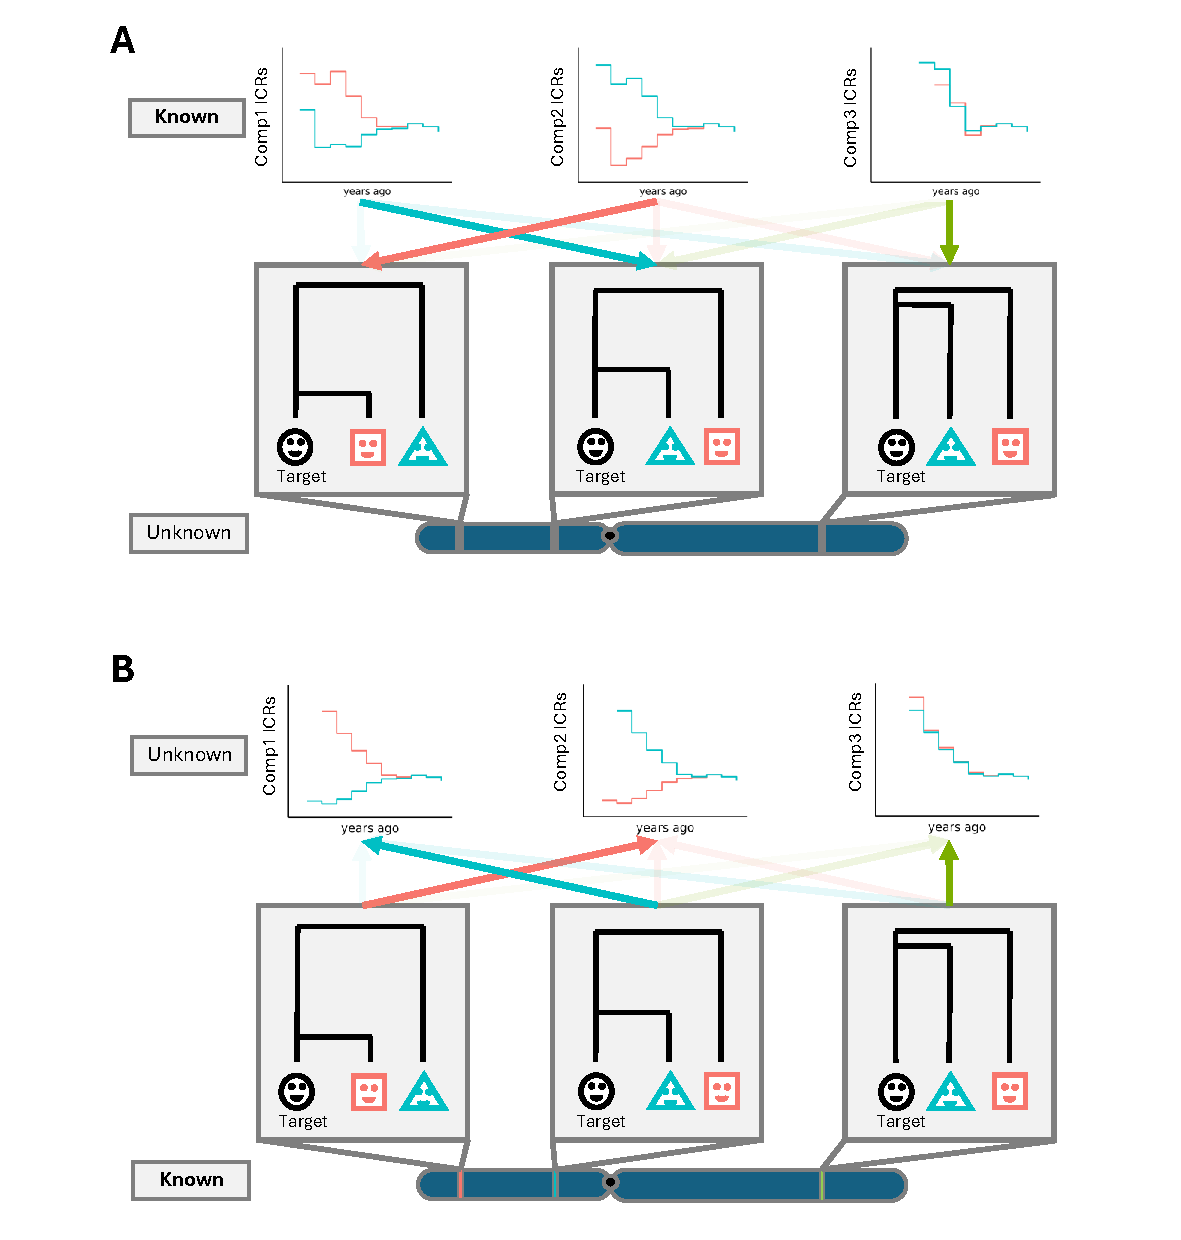
\includegraphics[width=\textwidth]{figures/thesis_gb_simplified_overview.pdf}
    \caption{\textbf{A simplified overview of GhostBuster.} GhostBuster implements an iterative expectation-maximization (EM) algorithm which cycles between two states A and B. (A) inferring local ancestry of a target individual given multiple coalescence rates of the target individuals with a set of reference populations. (B) using the local ancestry to refine the estimates of coalescence rates of target individual and the reference populations.}
    \label{fig:gb-simplified-overview}
\end{figure}

\section{Theoretical framework for our method}
\label{sec:ch2-gb-theory}

\subsection{Introduction to mixture models}

Mixture models are a general class of probabilistic models used to represent the presence of subpopulations within an overall population, even when there is no explicit identification of subpopulation membership for individual observations. Essentially, they assume that the data being analyzed is generated from a mixture of several different distributions, where each distribution corresponds to a different subpopulation or cluster. 

\subsubsection{Gaussian mixture models}

One of the simplest and most widely used mixture models is the Gaussian Mixture Model (GMM). Let's assume the data is sampled from a mixture of two Gaussian distributions with different means. The GMM assumes that each data point $\mathbf{x}$ is generated from one of these Gaussian distributions. Mathematically, the model is expressed as:
\begin{equation}
p(\mathbf{x}) = \pi_1 \mathcal{N}(\mathbf{x} \mid \mu_1, \Sigma_1) + \pi_2 \mathcal{N}(\mathbf{x} \mid \mu_2, \Sigma_2)
\end{equation}

where, $\pi_1$ and $\pi_2$ are the proportions of being in either one of the clusters, satisfying $\pi_1 + \pi_2 = 1$, and $(\mu_1, \Sigma_1)$ and $(\mu_2, \Sigma_2)$ are the parameters of the two Gaussians. Therefore the parameters to be inferred from the observed samples are $(\pi_1, \mu_1, \Sigma_1, \mu_2, \Sigma_2)$. The inference of the parameters is often carried out using the expectation-maximization (EM) algorithm \cite{dempster1977maximum}.

The EM algorithm operates by probabilistically inferring hidden variables under the model in the E-step, and using these hidden variables to simplify and analytically maximize the likelihood in the M-step. In the Gaussian Mixture Model, the hidden variables are the cluster memberships of each data point. The EM updates for Gaussian Mixture Models proceed as follows:

\begin{enumerate}
    \item E-step: Compute the expected log-likelihood of the data conditioned on the current estimates of the parameters. For Gaussian Mixture Models, this involves calculating the posterior probabilities that a data point belongs to a Gaussian distribution:
    \begin{equation}
        \gamma_{i}(\mathbf{x}_j) = \frac{\pi_i \mathcal{N}(\mathbf{x}_j \mid \mu_i, \Sigma_i)}{\sum_{k=1}^{2} \pi_k \mathcal{N}(\mathbf{x}_j \mid \mu_k, \Sigma_k)}
    \end{equation}
    where, $\gamma_{i}(\mathbf{x}_j)$ is the hidden variable that represents the probability that the data point $\mathbf{x}_j$ was generated by the $i$-th Gaussian distribution. 
    \item M-step: Uses the hidden variable to maximize the expected log-likelihood and estimate updated parameters:
    \begin{align}
        \pi_i^{\text{new}} &= \frac{1}{N} \sum_{j=1}^{N} \gamma_{i}(\mathbf{x}_j)  \nonumber \\
        \mu_i^{\text{new}} &= \frac{\sum_{j=1}^{N} \gamma_{i}(\mathbf{x}_j) \mathbf{x}_j}{\sum_{j=1}^{N} \gamma_{i}(\mathbf{x}_j)} \nonumber \\
        \Sigma_i^{\text{new}} &= \frac{\sum_{j=1}^{N} \gamma_{i}(\mathbf{x}_j) (\mathbf{x}_j - \mu_i^{\text{new}})(\mathbf{x}_j - \mu_i^{\text{new}})^\top}{\sum_{j=1}^{N} \gamma_{i}(\mathbf{x}_j)}
    \end{align}
\end{enumerate}

It can be shown that iterating between the E- and M-steps leads to non-decreasing log-likelihood updates. An illustration of the model fitting for a 2-dimensional mixture of Gaussians is shown in Figure \ref{fig:gb-gmm-visualize}.

\begin{figure}
    \centering
    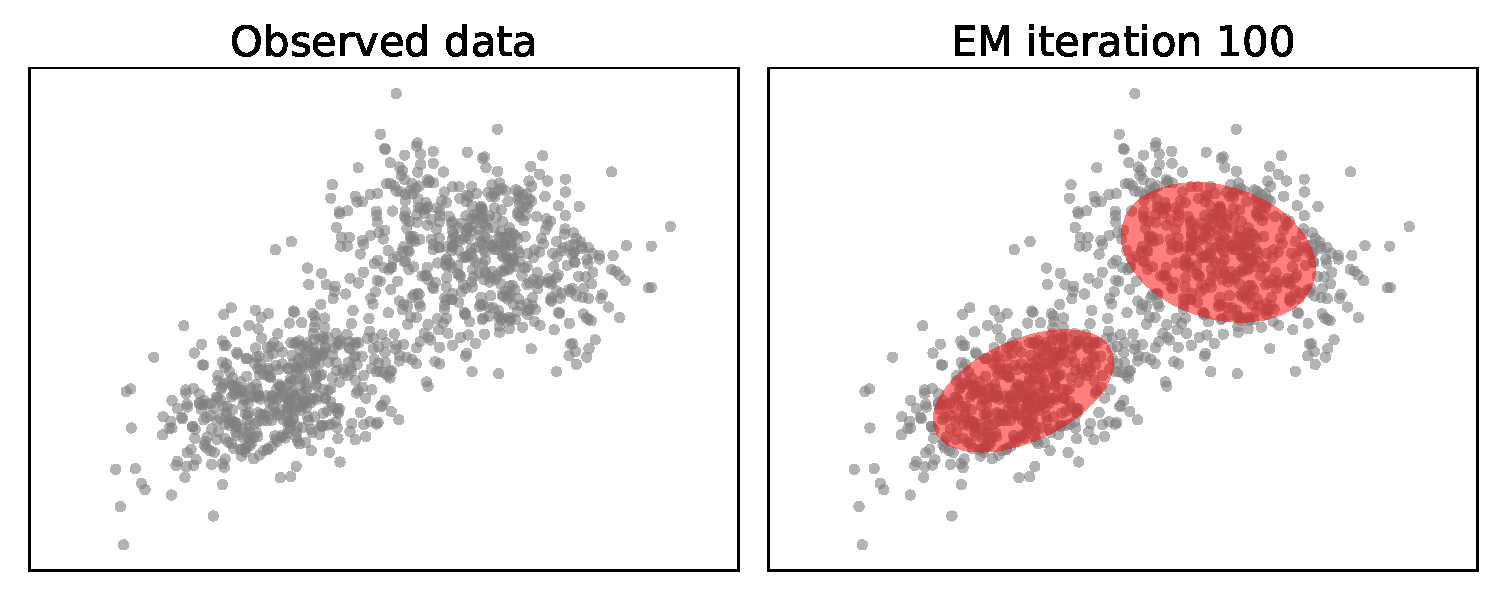
\includegraphics[width=\textwidth]{figures/gmm_visualize.pdf}
    \caption{\textbf{Gaussian mixture model.} The observed data and inferred clusters using the Gaussian mixture model after 100 EM iterations, the Gaussian mixtures inferred are represented by the red ellipse.}
    \label{fig:gb-gmm-visualize}
\end{figure}

\subsection{Mixture model for the coalescent}
\label{the_model}
We aim to extend the basic example of mixture models to genealogies by specifically modeling coalescence events on a given target lineage as a mixture distribution. The input for our method consists of at each site which individuals and at what times (or reference populations) the target sample coalesces as we move backward in time. Our goal is to model this as a mixture distribution, clustering locations based on `differences' in the coalescence histories of the target lineage. The expected output of our model is a per-component coalescence rate matrix, which defines how the target individual coalesces with a set of reference population within each specific component of the mixture.

Our method capitalizes on the fact that admixtures can be characterized by these coalescence rates with a set of reference populations. To illustrate this, consider the example of Denisovan admixture in Papuans. It is well known that Papuans carry up to 5\% Denisovan ancestry in their genomes. This archaic ancestry is distinct from the majority of Papuan ancestry, as the regions with Denisovan admixture exhibit more frequent coalescence events with Denisovans but do not coalesce with modern human lineages until the time of the Denisovan-human split. Therefore, there is a clear difference in the coalescence history between archaic and non-archaic genomic regions in Papuans, which we leverage to infer admixture.

We use the coalescent framework to model coalescence times along a lineage as an exponential distribution, where coalescence rates are determined by the population distribution of the clade coalescing with the target lineage. We have already derived a closed-form solution for the Maximum Likelihood Estimate (MLE) of coalescence rates for a pair of lineages (see Section \ref{sec:ch1-gb-theory}). This maximum likelihood estimate can be extended to multiple samples by treating each pair of lineages independently and multiplying the likelihood across all pairs. This approach is used to estimate effective population sizes and cross-population coalescence rates in PSMC \cite{li2011inference}, a widely used tool for inferring population history from genetic data. 

Although the pairwise likelihood approach is straightforward, it assumes that each pair of lineages is independent, even though they are highly structured and interdependent. To address this limitation, we extend the likelihood of observing coalescence events by conditioning on the inferred tree topology at each genomic site. More formally, we model the probability of a target lineage coalescing with any remaining lineage using a non-homogeneous Poisson process. To simplify the model, we assume that the coalescence rate of a lineage is proportional to the weighted sum of the coalescence rates of its descendants, as inferred from the tree at that site (see Figure \ref{fig1} for an example).

\begin{figure}[h!]
    \centering
    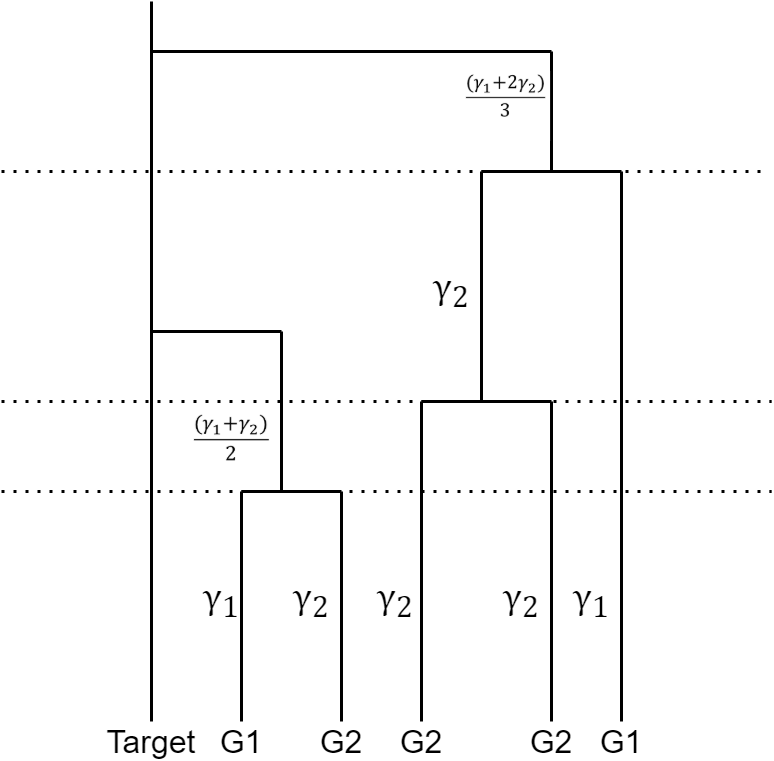
\includegraphics[scale=0.275]{figures/ghost buster simon myers-Page-1.png}
    \caption{Toy example showing how coalescence rates depends on the weighted sum of coalescence rates of the descendants}
    \label{fig1}
\end{figure}

The MLE of coalescence rates derived in section \ref{sec:ch1-gb-theory} also assumes independence of trees along the genome. To address this, we employ a Hidden Markov Model (HMM) to capture ancestry switches along the genome, treating each location Markovian. This approach mitigates the independence assumption and enhances the power of our likelihood estimation further.

\subsubsection{Likelihood of a single coalescence event}

Under our model, the probability distribution of observing a single coalescence event at time $t$ can be expressed as follows:
\begin{equation}
    P(t | \gamma) = \frac{\sum_{g=1}^R\gamma_{g}(m)n_{g}}{\sum_{g=1}^R n_{g}}e^{-\sum_{g=1}^R \gamma_{g} \cdot O_{g}}
\end{equation}
where, $n_{g} =$ number of group $g$ individuals coalescing in the coalescence event, $\gamma_{g}(m)$ is the corresponding coalescence rate of group $g$ in time epoch $m$ and, $O_{g}$ is the opportunity and equal to the sum of branch length from lower epoch boundary to the coalescence event corresponding to all group g individuals coalescing at $t$. This weighting corresponds to choosing which group to coalesce at a given coalescence event based on the proportion of descendants belonging to that particular group in that coalescence event. 

\subsection{EM derivation: the likelihood}
\subsubsection{Terminology}
\label{terminology}
We aim to fit a mixture model to cluster the genome based on variations in coalescence rates. To reduce computational costs, we divide the genome into $T$ small grids and focus on inferring local ancestry at these grid points, rather than at every individual location on the genome. Additionally, we approximate coalescence rates as piecewise constant functions over time, defined by $E$ time epochs that are equally spaced on a logarithmic scale. For the derivation of the EM algorithm, we use the following terminology:
\begin{itemize}    
    \item Our input data are the genealogies which contain:
    \begin{enumerate}
        \item $Q_l =$ Number of coalescence events with the target in $l^{th}$ grid
        \item $e_{li} =$ Epoch in which $i^{th}$ coalescent event happens in the $l^{th}$ grid
        \item $t_{li} =$ Coalescence time for the $i^{th}$ coalescence event in the $l^{th}$ grid
        \item $r_{l} =$ Genomic distance between $(l-1)^{th}$ and $l^{th}$ position along the genome
    \end{enumerate}

    \item The parameters we infer using are EM algorithm are:
    \begin{enumerate}
        \item $\gamma_{jg}(m) =$ Coalescence rate between reference group $g$ and the target in the $j^{th}$ mixture component and in epoch $m$
        \item $\pi_j  = P(z_l = j) =$ Cluster proportion of the $j^{th}$ mixture component
        \item $\lambda =$ Admixture time in generations 
    \end{enumerate}

    \item Lets define some fixed constants we will use in derivation:
    \begin{enumerate}
        \item $C =$ Total number of coalescence events in the ARG
        \item $T =$ Total number of grid points
        \item $A =$ Number of clusters assumed in the target
        \item $N_{li} =$ Number of reference individuals in $i^{th}$ coalescence event and $l^{th}$ grid
        \item $E =$ Number of time epochs (where the coalescence rates are assumed piece-wise constant)
    \end{enumerate}

    \item We will maintain consistency by using the same subscript to index the same variables throughout the derivation:
    \begin{enumerate}
        \item $l =$ Grid position along the genome
        \item $i =$ Coalescence event count
        \item $g =$ Pre-defined reference groups (e.g. Papuans, Denisovans, etc.)
        \item $j =$ Cluster or component in the mixture
        \item $e =$ Time epoch going backwards in time
    \end{enumerate}

    \item In the E-step, we introduce hidden variables to facilitate analytical updates. These variables are probabilistically inferred based on the current estimates of the parameters:
    \begin{enumerate}
        \item $z_l =$ Local ancestry of the target at position $l$
        \item $q_{li} =$ Reference individual index that coalesces in the $i^{th}$ coalescence event and $l^{th}$ grid
        \item $\omega_l =$ Number of recombinations since admixture between position $l-1$ and $l$
    \end{enumerate}

\end{itemize}

\subsubsection{The ``true'' likelihood}
We wish to formalize the likelihood for the mixture model described verbally in section \ref{the_model}. We write the likelihood of the mixture model as the product over all coalescence events with the target lineage in the ancestral recombination graph (ARG): 
\begin{equation}
    P (t,z,q \vert \gamma, \pi, \lambda) = \prod_{c=1}^{C} \prod_{j = 1}^A \prod_{g =1}^{R} \prod_{m = 1}^E P (t_c,z_c = j,q_c=g \vert \gamma, \pi, \lambda)^{I_{\{z_c = j\}} I_{\{q_c = g\}} I_{\{e_c = m\}}}
\label{true_likelihood1}
\end{equation}

Where, $t$ is the vector of observed coalescence times, $z$ and $q$ are hidden variables per coalescence event. It is important to note the coalescence events in a ARG can span more than one tree, especially branches lower in the tree are less likely to be affected due to recombination and thus last longer along the genome. Next, we introduce windowing the genome and appropriately scaling the likelihood to still get the above equation as follows:
\begin{equation}
    \footnotesize
    P(t,z,q \vert \gamma, \pi, \lambda) = \prod_{c=1}^{C} \prod_{j = 1}^A \prod_{g =1}^{R} \prod_{m = 1}^E \prod_{l =1}^{T} \left( P(t_c,z_c = j,q_c=g \vert \gamma, \pi, \lambda)^{I_{\{z_c = j\}} I_{\{q_c = g\}} I_{\{e_c = m\}}} \right) ^{\frac{I_{\{w_c = l\}}}{K_c}}
\label{true_likelihood2}
\end{equation}
where, $I_{\{w_c = l\}}$ is the indicator random variable indicating if the $l^{th}$ grid point overlaps with the branch corresponding to $c^{th}$ coalescence event, and $K_c$ is the total number of grids the branch corresponding to $c^{th}$ coalescence event lasts (we refer to this term as node persistence). We scale the likelihood in equation \ref{true_likelihood2} by $\frac{1}{K_c}$ such that it is still equal to the original likelihood in equation \ref {true_likelihood1}. 

\subsubsection{Accounting for uncertain coalescence events}

Genealogies inferred from genetic variation data come with the added complexity of uncertainty, as they are not always entirely accurate. The support for a particular node in the tree is stronger when there is a mutation mapped just above that node. To account for this uncertainty, we scale the likelihood by the confidence in each coalescence event. Specifically, as we move backward in time along the target lineage, we count the number of coalescence events that occur before encountering a mutation. All coalescence events between successive mutations are then weighted by one divided by the number of such events, effectively treating them as a single coalescence event. This adjustment improves the robustness of our method to errors in inferred genealogies, as demonstrated in empirical analyses. Overall this results in scaling the likelihood in equation \ref{true_likelihood2} by an additional term, $H_c$, which calculates the effective contribution of a coalescence event to the likelihood depending on its certainty. The updated likelihood is now given as: 
\begin{equation}
    \footnotesize
    P(t,z,q \vert \gamma, \pi, \lambda) = \prod_{c=1}^{C} \prod_{j = 1}^A \prod_{g =1}^{R} \prod_{m = 1}^E \prod_{l =1}^{T} \left( P(t_c,z_c = j,q_c=g \vert \gamma, \pi, \lambda)^{I_{\{z_c = j\}} I_{\{q_c = g\}} I_{\{e_c = m\}}} \right) ^{\frac{I_{\{w_c = l\}}}{B_c}}
\label{true_likelihood3}
\end{equation}
where, $B_c = \frac{H_c}{K_c}$ is the effective scaling factor accounting for branch persistence and certainty of coalescence events in inferred genealogies. Even though we divide the likelihood in different grids its not straight-forward to optimize the likelihood directly. In the next section, we approximate the likelihood in equation \ref{true_likelihood3} so that we can use Markov models for inference. 


\subsubsection{Markovian approximation to the ``true'' likelihood}
We perform a Markovian approximation to the ``true'' likelihood defined in equation \ref{true_likelihood3} and re-write the cluster membership $z$ in terms of window $l$ instead of coalescence event $c$. More formally we approximate as follows:
\begin{equation}
    P (t,z,q \vert \gamma, \pi, \lambda) \approx \prod_{l =1}^{T} \prod_{j = 1}^A \prod_{i = 1}^{Q_l} \prod_{k =1}^{N_{li}} \prod_{m = 1}^E \Big( P(t_{li}, q_{li} = k, z_l = j \vert \gamma, \pi, \lambda) ^ {I_{\{q_{l i} = k\}}  I_{\{e_{l i} = m\}}} \Big) ^{\frac{I_{\{z_l = j\}}}{B_{li}}}
    \label{markov_approx}
\end{equation}
where, $q_{li}$ is a hidden variable recording which reference individual the target coalesced with in the $i^{th}$ coalescence event at grid $l$. Similarly, $Q_{l}$ is the total number of coalescence events which overlap with grid point $l$ and $N_{li}$ is the list of reference individuals which coalesce at $q_{li}^{th}$ coalescence event. The Markovian assumption not only allows us to use markov models like HMMs for inference but also simplifies the cluster membership per position $l$ which can be easily interpreted as local ancestry at position $l$. We further simplify the equation \ref{markov_approx} and separate it into two parts.

\begin{equation}
    \footnotesize
    P (t,z,q \vert \gamma, \pi, \lambda) = \underbrace{P(z \vert \pi, \lambda)}_{\text{Term 2}} \prod_{l =1}^{T} \prod_{j = 1}^A \prod_{i = 1}^{Q_l} \prod_{k =1}^{N_{li}} \prod_{m = 1}^E \underbrace{\Big( P(t_{li}, q_{li} = k \vert z_l = j, \gamma) ^ {I_{\{q_{l i} = k\}}  I_{\{e_{l i} = m\}}} \Big) ^{\frac{I_{\{z_l = j\}}}{B_{li}}}}_{\text{Term 1}}
    \label{eq:term1_term2}
\end{equation}

We perform expectation-maximization and optimize term 1 to get the $\gamma$ (coalescence rates) and term 2 to get $\lambda$ (admixture time) and $\pi$ (global cluster proportions). In the following sections we simplify our calculations by deriving the EM updates for term 1 and term 2 separately. 

\subsection{EM derivation: inference of coalescence rates}
We write the likelihood term 1 in equation \ref{eq:term1_term2} which only depends on coalescence rates as follows: 
\begin{equation}
     P(t, q \vert z, \gamma) = \prod_{l = 1}^T \prod_{j = 1}^A \prod_{i = 1}^{Q_l} \prod_{k =1}^{N_{li}} \prod_{m = 1}^E   P(t_{li}, q_{l i} = k \vert z_l = j, \gamma) ^ {\frac{I_{\{z_l = j\}}I_{\{q_{l i} = k\}}  I_{\{e_{l i} = m\}}}{B_{li}}}
\label{eq:scaled_ll}
\end{equation}
where, The indicator random variables $I_{\{z_l = j\}}$, $I_{\{e_{l i} = m\}}$ and, $I_{\{q_{l i} = k\}}$ are present to simplify the equation when writing it down for all the trees and coalescence events in that tree. The log-likelihood is given by:

\begin{equation}
     \log P(t, z, q \vert \gamma) = \sum_{l = 1}^T \sum_{j = 1}^A \sum_{i = 1}^{Q_l} \sum_{k =1}^{N_{li}} \sum_{m = 1}^E  \frac{I_{\{q_{l i} = k\}} I_{\{z_l = j\}} I_{\{e_{l i} = m\}} \log P(t_{li}, q_{l i} = k \vert z_l = j, \gamma)}{B_{li}} 
\end{equation}

We can simplify the log-likelihood further as:
\begin{equation}
    P(q_{li} = k, t_{li} | z_l = j, \gamma ) = P(t_{li} | \gamma, z_l = j, q_{li} = k)P(q_{li} = k | z_l = j, \gamma)
\end{equation}

\begin{enumerate}
    \item Looking at the first term $P(t_{li} | \gamma, z_l = j, q_{li} = k)$:
\begin{align}
    P(t_{li} | \gamma, z_l = j, q_{li} = k) = P(t_{li} | \gamma, z_l = j) \nonumber \\
    P(t_{li} | \gamma, z_l = j) = \frac{\sum_{g=1}^R\gamma_{jg}(m)n_{lig}}{\sum_{g=1}^R n_{lig}}e^{-\sum_{g=1}^R \gamma_{jg} \cdot O_{lg}[i]}
\end{align}
where, $n_{lig} =$  number of group $g$ individuals coalescing in the $i^{th}$ coalescence event and position $l$ and, $O_{lg}[i] =$ sum of branch length from lower epoch boundary to the $i^{th}$ coalescence event corresponding to all group g individuals coalescing at $t_{li}$.
\vspace{3mm}
\item The second term $P(q_{li} = k | z_l = j, \gamma)$ simplifies to:
\begin{equation}
    P(q_{li} = k | z_l = j, \gamma) = \frac{\gamma_{jg(k)}(m)C_{ik}\sum_{g=1}^Rn_{lig}}{\sum_{g=1}^R \gamma_{jg}(m)n_{lig}}
\label{eq:qli}
\end{equation}

where, $g(k)$ means the group assignment (among $R$ groups) of the $k^{th}$ individual in the reference panel, and $C_{ik}$ is the contribution of $k^{th}$ individual in $i^{th}$ lineage. 
\end{enumerate}

Overall $P(q_{li} = k, t_{li} | z_l = j, \gamma )$ can be written as: 
\begin{align}
    P(q_{li} = k, t_{li} | \gamma, z_l = j ) = \gamma_{jg(k)}(m)C_{ik}e^{-\sum_{g=1}^R \gamma_{jg}\cdot O_{lg}[i]} \nonumber \\
    \propto \gamma_{jg(k)}(m)*e^{-\sum_{g=1}^R \gamma_{jg}\cdot O_{lg}[i]}
    \label{eq:likelihood}
\end{align}

We can maximize the likelihood corresponding to term 1 through an expectation-maximization algorithm. Where, in the E-step we define the expected log-likelihood of the data given the hidden variables and the previous estimates of the parameters (including $\lambda$ and $\pi$), and in the M-step we maximize this expected log-likelihood. Under the expectation maximization framework, it is guaranteed the likelihood is going to increase every iteration thereby guaranteeing convergence to a local minima. Next, we derive the E-step and M-step for our likelihood in equation \ref{eq:likelihood}.
 
\subsubsection{E-step}

In the E-step we calculate the expected log-likelihood, where the expectation is w.r.t the hidden variables conditioned on the data and previous parameter estimation. We therefore proceed by stating the expected log-likelihood in our case:
\begin{equation}
   E_{z, q | \gamma^{t-1}, \lambda^{t-1}, \pi^{t-1}, t} \Big(  \sum_{l = 1}^T \sum_{j = 1}^A \sum_{i = 1}^{Q_l} \sum_{k =1}^{N_{li}} \sum_{m = 1}^E  \frac{I_{\{q_{l i} = k\}} I_{\{z_l = j\}} I_{\{e_{l i} = m\}} \log P(t_{li}, q_{l i} = k \vert z_l = j, \gamma)}{B_{li}} \Big)
 \end{equation}

We start simplifying the expected log-likelihood by taking the expectation inside the summation, and transforming the expected value of indicator random variables as probabilities.  
\begin{footnotesize}
\begin{align}
    &= \sum_{l = 1}^T \sum_{j = 1}^A  \sum_{i = 1}^{Q_l} \sum_{k =1}^{N_{li}} \sum_{m = 1}^E P(q_{li} = k, z_l = j \mid \gamma^{t-1}, \lambda^{t-1}, \pi^{t-1}, t) I_{\{e_{l i} = m\}} \frac{\log(P(q_{l i} = k, t_{li} \mid z_l = j, \gamma ))}{B_{li}}
\end{align}
\end{footnotesize}

Simplifying further and substituting the value of $log(P( q_{l i} = k, t_{li} | z_l = j, \gamma ))$ from equation \ref{eq:likelihood}. Note, we omit the constants of proportionality as they do not depend on the coalescence rates and thus will not affect the maximization in the M-step.
\begin{align}
    &= \sum_{l = 1}^T \sum_{j = 1}^A \sum_{i = 1}^{Q_l} \sum_{k = 1}^{N_{li}} \sum_{m = 1}^E \Bigg( 
        P(q_{li} = k \mid \gamma^{t-1}, t, z_l = j) P(z_l = j \mid t, \gamma^{t-1}, \lambda^{t-1}, \pi^{t-1}) \nonumber \\
    &\quad \times I_{\{e_{l i} = m\}} \frac{\log(P(q_{l i} = k, t_{li} \mid z_l = j, \gamma))}{B_{li}} \Bigg) \nonumber \\
    &= \sum_{l = 1}^T \sum_{j = 1}^A \sum_{i = 1}^{Q_l} \sum_{k = 1}^{N_{li}} \sum_{m = 1}^E \Bigg( 
        P(q_{li} = k \mid \gamma^{t-1}, t, z_l = j) P(z_l = j \mid t, \gamma^{t-1}, \lambda^{t-1}, \pi^{t-1}) \nonumber \\
    &\quad \times I_{\{e_{l i} = m\}} \frac{\log(\gamma_{jg(k)}(m)) - \sum_{g=1}^R \gamma_{jg} \cdot O_{lg}[i]}{B_{li}} \Bigg) 
\end{align}

Note the probability of $q_{li}$ (as defined in equation \ref{eq:qli}) does not depend on admixture time and proportion. We can simplify the expected log-likelihood further and switch the individual assignment hidden variable $q_{li}$ to more easily computable group assignment hidden variable $q'_{li}$. 
\begin{align}
   &\color{red}{\sum_{l = 1}^T \sum_{j = 1}^A \sum_{i = 1}^{Q_l} \sum_{k = 1}^{N_{li}} \sum_{m = 1}^E \Bigg( 
       P(q_{li} = k \mid \gamma^{t-1}, z_l = j) P(z_l = j \mid t, \gamma^{t-1}, \lambda^{t-1}, \pi^{t-1})} \nonumber \\
   &\quad \color{red}{\times I_{\{e_{l i} = m\}} \frac{\log(\gamma_{jg(k)}(m))}{B_{li}} \Bigg)} \nonumber \\
   &\color{blue}{- \sum_{l = 1}^T \sum_{j = 1}^A \sum_{i = 1}^{Q_l} \sum_{k = 1}^{N_{li}} \sum_{m = 1}^E \Bigg( 
       P(q_{li} = k \mid \gamma^{t-1}, z_l = j) P(z_l = j \mid t, \gamma^{t-1}, \lambda^{t-1}, \pi^{t-1})} \nonumber \\
   &\quad \color{blue}{\times I_{\{e_{l i} = m\}} \frac{\sum_{g=1}^R \gamma_{jg} \cdot O_{lg}[i]}{B_{li}} \Bigg)}
\end{align}

We group the individuals based on group assignment in the first term (red term) and use $\sum_{k =1}^{N_{li}} P(q_{li} = k | \gamma^{t-1}, z_l = j) = 1$ in the second term (blue term). 
\begin{align}
   &\color{red}{\sum_{l = 1}^T \sum_{j = 1}^A \sum_{i = 1}^{Q_l} \sum_{k = 1}^{N_{li}} \sum_{m = 1}^E \Bigg( 
       P(q'_{li} = g \mid \gamma^{t-1}, z_l = j) P(z_l = j \mid t, \gamma^{t-1}, \lambda^{t-1}, \pi^{t-1})} \nonumber \\
   &\quad \color{red}{\times I_{\{e_{l i} = m\}} \frac{\log(\gamma_{jg}(m))}{B_{li}} \Bigg)} \nonumber \\
   &\color{blue}{- \sum_{l = 1}^T \sum_{j = 1}^A \sum_{i = 1}^{Q_l} \sum_{m = 1}^E \Bigg( 
       P(z_l = j \mid t, \gamma^{t-1}, \lambda^{t-1}, \pi^{t-1}) I_{\{e_{l i} = m\}}}  \sum_{g=1}^R \frac{\gamma_{jg} \cdot O_{lg}[i]}{B_{li}} \Bigg)
   \label{estep:ell-simple}
\end{align}

Lets denote $U_{l,i,g,j,m}^{t-1}$ as the first term corresponding to the membership ``group g individual coalesces in the $i^{th}$ coalescence event''. And, lets denote $T_{l,j}^{t-1}$ as the second term corresponding to the local ancestry of the target. We use the forward-backward algorithm for HMM to evaluate $T_{l,j}$ in future section \ref{sec:term2_estep}. Whereas, we calculate $U_{l,i,g,j,m}^{t-1}$ based on our model as follows:
\begin{equation}
    U_{l,i,g,j,m}^{t-1} = P(q'_{li} = g | \gamma^{t-1}, z_l = j) = \frac{\gamma_{jg}^{t-1}(m)c_{lig}}{\sum_{g=1}^R \gamma_{jg}^{t-1}(m)c_{lig}}
    \label{estep:u}
\end{equation}
where, $c_{lig} = \frac{n_{lig}}{\sum_{g=1}^R n_{lig}}$ are the normalized proportions of coalescence count for each coalescence event

\subsubsection{M-step}

Once we have the expected log-likelihood we can maximize it in the M-step. We substitute $U_{l,i,g,j,m}^{t-1}$ and $T_{l,j}^{t-1}$ as hidden variables from equation \ref{estep:u} and HMM forward-backward into equation \ref{estep:ell-simple}. We Maximize w.r.t $\gamma_{jg}(m)$ as follows:
\begin{align}
    &\sum_{l = 1}^T \sum_{i = 1}^{Q_l} \sum_{j = 1}^A \sum_{g = 1}^R \sum_{m = 1}^E \Bigg( 
        U_{l,i,g,j,m}^{t-1} T_{l,j}^{t-1} I_{\{e_{l i} = m\}} \frac{\log(\gamma_{jg}(m))}{B_{li}} \Bigg) \nonumber \\
    &- \sum_{l = 1}^T \sum_{i = 1}^{Q_l} \sum_{j = 1}^A \sum_{m = 1}^E \Bigg( 
        T_{l,j}^{t-1} I_{\{e_{l i} = m\}} \sum_{g = 1}^R \frac{\gamma_{jg} \cdot O_{lg}[i]}{B_{li}} \Bigg)
\end{align}

Differentiating w.r.t $\gamma_{jg}(m)$ and setting it to 0 we get:
\begin{equation}
\sum_{l = 1}^T \sum_{i = 1}^{Q_l}  \Big( \frac{I_{\{e_{l i} = m\}}U_{l,i,g,j,m}^{t-1} T_{l,j}^{t-1}}{\gamma_{jg}(m)B_{li}} \Big) -  \sum_{l = 1}^T \sum_{i = 1}^{Q_l} \Big(\frac{I_{\{e_{l i} = m\}} T_{l,j}^{t-1}  O_{lg}[i]}{B_{li}} \Big) = 0
\end{equation} 

% \begin{equation}
% \sum_{l = 1}^T \sum_{i = 1}^{Q_l}  \Big( \frac{I_{\{e_{l i} = m\}}U_{l,i,g,j,m}^{t-1} T_{l,j}^{t-1}}{\gamma_{jg}(m)} \Big) =  \sum_{l = 1}^T \sum_{i = 1}^{Q_l} \Big(I_{\{e_{l i} = m\}} T_{l,j}^{t-1}  O_{lg}[i] \Big)
% \end{equation} 
\begin{align}
    \gamma_{jg}^{t}(m) &= \frac{\sum_{l = 1}^T \sum_{i = 1}^{Q_l}  I_{\{e_{l i} = m\}} U_{l,i,g,j,m}^{t-1} T_{l,j}^{t-1}/B_{li}}{\sum_{l = 1}^T \sum_{i = 1}^{Q_l}  I_{\{e_{l i} = m\}} T_{l,j}^{t-1}  O_{lg}[i]/B_{li} } \nonumber \\
    \gamma_{jg}^{t}(m) &= \frac{\sum_{l = 1}^T \sum_{i = 1}^{Q_l}  I_{\{e_{l i} = m\}} \frac{\gamma_{jg}^{t-1}(m)c_{lig}}{\sum_{g=1}^R \gamma_{jg}^{t-1}(m)c_{lig}} T_{l,j}^{t-1}/B_{li}}{\sum_{l = 1}^T \sum_{i = 1}^{Q_l}  I_{\{e_{l i} = m\}} T_{l,j}^{t-1}  O_{lg}[i]/B_{li} }
\label{eq:gamma_update}
\end{align}
where, $Opp_{lg}(m)$ is the sum of branch length in epoch $m$. It is important to note we do not need to store $U_{l,i,g,j,m}^{t-1}$ explicitly, we can instead store $\gamma^{t-1}$ to save memory.

\subsection{EM derivation: inference for admixture time \& proportions}
% \textbf{Simplifying the log-likelihood of term 2} 

We assume a markov model to write the likelihood for term 2 in equation \ref{eq:term1_term2}. Apart from the local ancestry hidden variable ($z$) we also introduce another hidden variable, $\omega_l$ to record the number of recombination events since admixture between $l-1$ and $l$. We assume a user-defined recombination map is available, reporting distance between two grid points in genomic position as $r_l$. The likelihood of the term can then be written as follows:
\begin{equation}
    P(z, \omega_l \vert \lambda, \pi) \propto \prod\limits_{l=1}^{T} \Big( \prod\limits_{j=1}^{A} \pi_j ^ {I\{z_l = j\} I\{\omega_l > 0\}} \Big) (\lambda r_l)^{\omega_l} e^{-\lambda r_l}
\end{equation}
where, $z_l$ is local ancestry at position $l$, $\omega_l$ is the hidden variable recording the number of recombinations between site $l-1$ and $l$ since the admixture time and $r_l$ is the user-defined recombination rate at position $l$. The likelihood for the number of recombinations is given by a Poisson counting process. It is important to note, the local ancestry change happens if there is atleast a recombination event. The parameters of the model are $\lambda$, which is the admixture time and $\pi$ which are the global cluster proportions. The log-likelihood can be written as follows:
\begin{equation}
    \log P(z, \omega_l \vert \lambda, \pi) = \sum\limits_{l=1}^{T} \Big( \sum\limits_{j=1}^{A} I\{z_l = j\} I\{\omega_l > 0\} \log \pi_j \Big) + \omega_l \log \lambda r_l - \lambda r_l + \text{constants}
\end{equation}

\subsubsection{E-step}
\label{sec:term2_estep}

In order to perform EM, we look at the expected log-likelihood of the data where the expectation is taken with respect to the hidden variables conditioned on the data (coalescence times with the target) and previous iteration's model parameters (including the $\gamma$).
\begin{equation}
    E_{z, \omega_l \vert \gamma^{t-1}, \lambda^{t-1}, \pi^{t-1}, t}\Big( \sum\limits_{l=1}^{T} \Big( \sum\limits_{j=1}^{A} I\{z_l = j\} I\{\omega_l > 0\} \log \pi_j \Big) + \omega_l \log \lambda r_l - \lambda r_l \Big)
\end{equation}

We start simplifying the expected log-likelihood by taking the expectation inside the summation, and transforming the expected value of indicator random variables as probabilities. 
\begin{equation}
     \sum\limits_{l=1}^{T} \Big( \sum\limits_{j=1}^{A} P(z_l = j, \omega_l > 0 \vert \gamma^{t-1}, \lambda^{t-1}, \pi^{t-1}, t) \log \pi_j \Big) + E(\omega_l) log \lambda r_l - \lambda r_l
\end{equation}

where, the expectation is taken over the hidden variables conditioned on the data and previous iterations' parameter updates. We are interested to infer three terms, (1) $P(z_l = j, \omega_l > 0)$, (2) $E(\omega_l)$ and (3) $P(z_l = j | t, \gamma^{t-1}, \lambda^{t-1}, \pi^{t-1})$. We start with the first term:
\begin{align}
    P&(z_l = j, \omega_l > 0 \vert P^{t-1}, t) = P(z_l = j \vert P^{t-1}, t) P(\omega_l > 0 \vert z_l = j, P^{t-1}, t) \nonumber \\
    &= P(z_l = j \vert P^{t-1}, t) \sum\limits_{i=1}^{A} P(\omega_l > 0 \vert z_l = j, z_{l-1} = i, P^{t-1}, t) P(z_{l-1} = i \vert z_l = j, P^{t-1}, t) \nonumber \\
    &= \sum\limits_{i=1}^{A} P(z_l = j \vert P^{t-1}, t) P(\omega_l > 0 \vert z_l = j, z_{l-1} = i, P^{t-1}, t) P(z_{l-1} = i \vert z_l = j, P^{t-1}, t) \nonumber \\
    &= \sum\limits_{i=1}^{A} \color{red}{P(\omega_l > 0 \vert z_l = j, z_{l-1} = i, P^{t-1})} \color{blue}{P(z_l = j, z_{l-1} = i \vert P^{t-1}, t)}
\label{eq:hmm_estep}
\end{align}
where, $P^{t-1} = (\gamma^{t-1}, \lambda^{t-1}, \pi^{t-1})$ is a short-hand for the tuple of all previous parameters. We denote the second term (coloured in blue) as $\epsilon_{ij}(l)$ as it denotes the probability of being in state $i$ and state $j$ at position $l-1$ and $l$ respectively. Similar to the Baum-Welch algorithm we can solve for $\epsilon_{ij}(l)$ through the forward backward pass in hidden markov models. 

\begin{footnotesize}
\begin{align}
    &\epsilon_{ij}(l) =P(z_l = j, z_{l-1} = i \vert P^{t-1}, t) \nonumber \\
    &= \frac{P(z_l = j, z_{l-1} = i, t \vert P^{t-1})}{P(t \vert P^{t-1})} \nonumber \\
    &= \frac{P(t_1 .., t_{l-1}, z_{l-1}=i \vert P^{t-1}) P(z_l=j \vert z_{l-1}=i, P^{t-1}) P(t_{l} .., t_T \vert z_l=j, P^{t-1}) P(t_l \vert z_l, P^{t-1})}{P(t \vert P^{t-1})} \nonumber \\
    &= \frac{P(t_1 .., t_{l-1}, z_{l-1}=i \vert P^{t-1}) P(z_l=j \vert z_{l-1}=i, P^{t-1}) P(t_{l} .., t_T \vert z_l=j, P^{t-1}) P(t_l \vert z_l, P^{t-1})}{\sum\limits_{j=1}^{A}\sum\limits_{i=1}^{A} P(t_1 .., t_{l-1}, z_{l-1}=i \vert P^{t-1}) P(z_l=j \vert z_{l-1}=i, P^{t-1}) P(t_{l} .., t_T \vert z_l=j, P^{t-1}) P(t_l \vert z_l, P^{t-1})}
\label{eq:epsilon_ij}
\end{align}
\end{footnotesize}
where, $P(t_1 .., t_{l-1}, z_{l-1}=i \vert P^{t-1})$ is called the forward-pass and $P(t_{l} .., t_T \vert z_l=j, P^{t-1})$ is called the backward-pass. The transition probability for the HMM is given as follows:
\begin{equation}
     P(z_l=j \vert z_{l-1}=i, P^{t-1}) = \begin{cases} (1 - e^{-r_l \lambda^{t-1}})\pi_j^{t-1}, & \text{if } i \neq j \\ e^{-r_l \lambda^{t-1}} + (1 - e^{-r_l \lambda^{t-1}})\pi_j^{t-1} , & \text{if } i = j \end{cases}
\end{equation}

Whereas the emission probability for the HMM $P(t_l \vert z_l, P^{t-1})$ only depends on $\gamma^{t-1}$ and follows from the scaled likelihood in equation \ref{eq:scaled_ll}:
\begin{equation}
   P(t_l \vert z_l, P^{t-1}) =  \Big( \frac{\sum_{g=1}^R\gamma^{t-1}_{jg}(m)n_{lig}}{\sum_{g=1}^R n_{lig}}e^{-\sum_{g=1}^R \gamma^{t-1}_{jg} \cdot O_{lg}[i]} \Big)^{\frac{1}{B_{li}}}
\end{equation}

The first term (red coloured) in equation \ref{eq:hmm_estep} can be thought as the probability of atleast one recombination event conditioned on local ancestry around it being $z_{l-1}$ and $z_l$. It is given as follows:
\begin{equation}
  P(\omega_l > 0 \vert z_l = j, z_{l-1} = i, P^{t-1}) = \begin{cases} 1, & \text{if } i \neq j \\ \frac{(1 - e^{-r_l \lambda^{t-1}})\pi_j^{t-1}}{e^{-r_l \lambda^{t-1}} + (1 - e^{-r_l \lambda^{t-1}})\pi_j^{t-1}} , & \text{if } i = j \end{cases}
\label{eq:e_of_recomb>0}
\end{equation}

The next term which needs to be calculated in the E-step is $E(\omega_l)$ where the expectation is with respect to the hidden variables $z_l, \omega_l$ conditioned on the data and previous iteration's model parameters. We can simplify the expectation as follows:
\begin{align}
    E(\omega_l \vert P^{t-1}, t) &= E(\omega_l \vert \omega_l > 0, P^{t-1}, t) P( \omega_l > 0 \vert P^{t-1}, t) \nonumber \\
    &= E(\omega_l \vert \omega_l > 0, P^{t-1}) P( \omega_l > 0 \vert P^{t-1}, t) \nonumber \\
    &= \frac{\lambda^{t-1}r_l}{1 - e^{-\lambda^{t-1}r_l}} P( \omega_l > 0 \vert P^{t-1}, t)
\label{eq:estep_121}
\end{align}
where, $P^{t-1} = (\gamma^{t-1}, \lambda^{t-1}, \pi^{t-1})$ is a short-hand for the tuple of all previous parameters. In order to evaluate $ P( \omega_l > 0 \vert P^{t-1}, t)$ we do the following: 
\begin{align}
  P( \omega_l > 0 \vert P^{t-1}, t) &= \sum\limits_{j=1}^{A}\sum\limits_{j=1}^{A}  P( \omega_l > 0 \vert z_l = j, z_{l-1} = i, P^{t-1}, t) P(z_l = j, z_{l-1} = i \vert P^{t-1}, t) \nonumber \\
  &= \sum\limits_{j=1}^{A}\sum\limits_{j=1}^{A}  P( \omega_l > 0 \vert z_l = j, z_{l-1},  P^{t-1} = i) \epsilon_{ij}(l)
\label{eq:e_of_recomb}
\end{align}

We have already calculated the terms needed in equation \ref{eq:e_of_recomb} before in equation \ref{eq:epsilon_ij} and \ref{eq:e_of_recomb>0}. Lastly to calculate the local ancestry estimate $P(z_l = j | t, \gamma^{t-1}, \lambda^{t-1}, \pi^{t-1})$ needed in equation \ref{eq:gamma_update} we perform a forward-backward pass:
\begin{equation}
    P(z_l = j | t, \gamma^{t-1}, \lambda^{t-1}, \pi^{t-1}) = \frac{P(t_1 .., t_{l-1}, z_{l-1}=i \vert P^{t-1})P(t_{l} .., t_T \vert z_l=j, P^{t-1})}{\sum\limits_{j=1}^{A}P(t_1 .., t_{l-1}, z_{l-1}=i \vert P^{t-1})P(t_{l} .., t_T \vert z_l=j, P^{t-1})}
\label{eq:hmm_forward_backward}
\end{equation}
where, $P(t_1 .., t_{l-1}, z_{l-1}=i \vert P^{t-1})$ and $P(t_{l} .., t_T \vert z_l=j, P^{t-1})$ is the forward and backward probability respectively. 

\subsubsection{M-step}

Once we know all the necessary equations in E-step we proceed to maximize the expected log-likelihood in M-step. We maximize w.r.t $\lambda$ and cluster proportions $\pi$ by maximizing the equation below: 
\begin{equation}
    \sum\limits_{l=1}^{T}  \color{red}{ \Big( \sum\limits_{j=1}^{A} P(z_l = j, \omega_l > 0 \vert \gamma^{t-1}, \lambda^{t-1}, \pi^{t-1}, t) \log \pi_j} \Big) + \color{blue}{E(\omega_l) log \lambda r_l - \lambda r_l }
\end{equation}

\begin{enumerate}
    \item Differentiating w.r.t $\pi_j$ and setting to zero we get:  
    \begin{align}
        \pi^{t}_j &\propto \sum\limits_{l=1}^{T} P(z_l = j, \omega_l > 0 \vert \gamma^{t-1}, \lambda^{t-1}, \pi^{t-1}, t) \nonumber \\
        \pi^{t}_j &= \frac{\sum\limits_{l=1}^{T} P(z_l = j, \omega_l > 0 \vert \gamma^{t-1}, \lambda^{t-1}, \pi^{t-1}, t)}{\sum\limits_{j=1}^{A} \sum\limits_{l=1}^{T} P(z_l = j, \omega_l > 0 \vert \gamma^{t-1}, \lambda^{t-1}, \pi^{t-1}, t)}
    \label{eq:pi_updates}
    \end{align}
    
    We get the term $P(z_l = j, \omega_l > 0 \vert \gamma^{t-1}, \lambda^{t-1}, \pi^{t-1}, t)$ from the E-step equation \ref{eq:hmm_estep}. 
    \item Differentiating w.r.t $\lambda$ and setting to zero we get:
    \begin{equation}
        \lambda^t = \frac{\sum\limits_{l=1}^{T}E(\omega \vert \gamma^{t-1}, \lambda^{t-1}, \pi^{t-1}, t)}{\sum\limits_{l=1}^{T}r_l}
    \label{eq:lambda_updates}
    \end{equation}
    
    Note we get the expected number of recombinations from equation \ref{eq:estep_121} in E-step.
    
\end{enumerate}

\clearpage

\subsection{Summary of the algorithm}
We present a summary of the EM algorithm for GhostBuster here:

\begin{algorithm}
\caption{EM Algorithm for GhostBuster}
\begin{algorithmic}[1]
\State \textbf{Input:} Geneologies $\mathbf{X} = \{(t_1,n_1), (t_2,n_2), \dots, (t_C,n_C)\}$ containing coalescence times and population counts for each coalescence event, number of components $A$, number of time epochs $E$, number of grid points $T$, total number of coalescence events $C$ and $R$ is the number of reference groups.
\State \textbf{Preprocessing:} Calculate likelihood scaling term $B_c$ for each coalescence event $c = 1, 2, \dots, C$, and $r_l$ genetic distance between two grid points
\State \textbf{Initialize:} Coalescence rates $\gamma_j^{(0)}$, mixing coefficients $\pi_j^{(0)}$ for each component $j = 1, 2, \dots, A$ and admixture time $\lambda^{(0)}$ 
\State \textbf{Set:} Iteration $t = 0$

\Repeat

    \State \textbf{E-step:} 
    
    \For{each component $j = 1, 2, \dots, A$}

    \For{each data point $(t_{li}, n_{li})$}
    
            \Comment{$t_{li}$ represent the coalescence time in $l^{th}$ grid and $i^{th}$ coalescence event}
            
            \Comment{$t_{li}$ represent the coalescence time in $l^{th}$ grid and $i^{th}$ coalescence event}
            
            \Comment{$P^{t-1} = \{\gamma^{t-1}, \lambda^{t-1}, \pi^{t-1}\}$}

            \vspace{2mm}
            
            \State Compute the likelihood under the component:
            \[
               P(t_l \vert z_l, P^{t-1}) =  \Big( \frac{\sum_{g=1}^R\gamma^{t-1}_{jg}(m)n_{lig}}{\sum_{g=1}^R n_{lig}}e^{-\sum_{g=1}^R \gamma^{t-1}_{jg} \cdot O_{lg}[i]} \Big)^{\frac{1}{B_{li}}}
            \]
        \EndFor
        
        \State Perform forward-backward pass with the HMM to get $P(z_l = j | X, P^{t-1})$ 

        \hspace{7mm} see equation \ref{eq:hmm_forward_backward}

        
    \EndFor
    
    \State \textbf{M-step:}
    \For{each component $k = 1, 2, \dots, A$}
        \State Update the coalescence rates:
        
        \hspace{7mm} see equation \ref{eq:gamma_update}

        \State Update the mixing coefficient:
        
        \hspace{7mm} see equation \ref{eq:pi_updates}
        
        \State Update the admixture time:
        
        \hspace{7mm} see equation \ref{eq:lambda_updates}
            
    \EndFor
    
    % \State \textbf{Compute:} Log-likelihood:
    % \[
    % \mathcal{L}^{(t+1)} = \sum_{i=1}^{N} \log \left( \sum_{k=1}^{K} \pi_k^{(t+1)} \mathcal{N}(x_i \mid \mu_k^{(t+1)}, \Sigma_k^{(t+1)}) \right)
    % \]

    % \State \textbf{Check for convergence:} If $|\mathcal{L}^{(t+1)} - \mathcal{L}^{(t)}| < \epsilon$, stop.
    \State \textbf{Increment:} $t = t + 1$
    
\Until{convergence}

\State \textbf{Output:} Final parameters $\{\gamma^{t}, \lambda^{t}, \pi^{t}\}$ for $k = 1, 2, \dots, A$

\end{algorithmic}
\end{algorithm}

\section{Method description}
\label{sec:ch2-gb-method}
\subsection{Overview of the method}

GhostBuster is a mixture model that clusters local trees in the genealogy based on coalescence rates between target lineage and a set of reference populations.
%
It relies on the assumption that an admixture or gene-flow event can be well characterized by these coalescence rates with reference populations.  
%
GhostBuster uses the genealogies inferred using large-scale genealogy inference softwares like Relate \cite{speidel2019method} directly and fits the mixture model using an iterative expectation maximization (EM) algorithm.
%
For this manuscript we restrict ourselves to Relate due to its scalability to thousands of samples and higher accuracy compared to other genealogy inference methods \cite{brandt2022evaluation}, but there is no conceptual difference in using our method with other genealogy inference methods.

The algorithm starts with a fixed number of mixture components (which is user-specified) and randomly initializing the admixture time and per-component genome-wide proportions and coalescence rates. 
%
The proportions are enforced to sum to one, whereas the coalescence rates are calculated with each reference population as a piece-wise constant function of time. 
%
In the E-step, GhostBuster calculates the expected log-likelihood of the data (in our case the coalescence time with reference individuals) conditioned on the local tree topology and previous estimates of the model parameters (proportions, admixture time and coalescence rates). 
%
We then use a hidden Markov model (HMM) to infer the local ancestry of the target individual.
%
The emissions for the HMM are modelled using the likelihood of the coalescence times, whereas the transitions are modelled using a Poisson process depending on recombination rates. 

In the M-step, we maximize the expected log-likelihood calculated in the E-step to get a new estimate of the model parameters. 
%
Under the EM algorithm, we are guaranteed this leads to non-decreasing likelihood updates and therefore a local optima \cite{dempster1977maximum}. 
%
The likelihood we derive conditions on the tree topology by carefully counting lineage contribution based on its descendants and leads to a higher statistical power to detect admixture events in our analysis, as we do not assume reference individuals are independent or use any composite likelihood assumptions.
%
A more detailed proof of the likelihood and the EM algorithm updates can be found in section \ref{sec:ch2-gb-theory}. 

A graphic overview of the method can be found in Figure \ref{fig:gb_overview}.

\begin{figure}[h!]
    \centering
    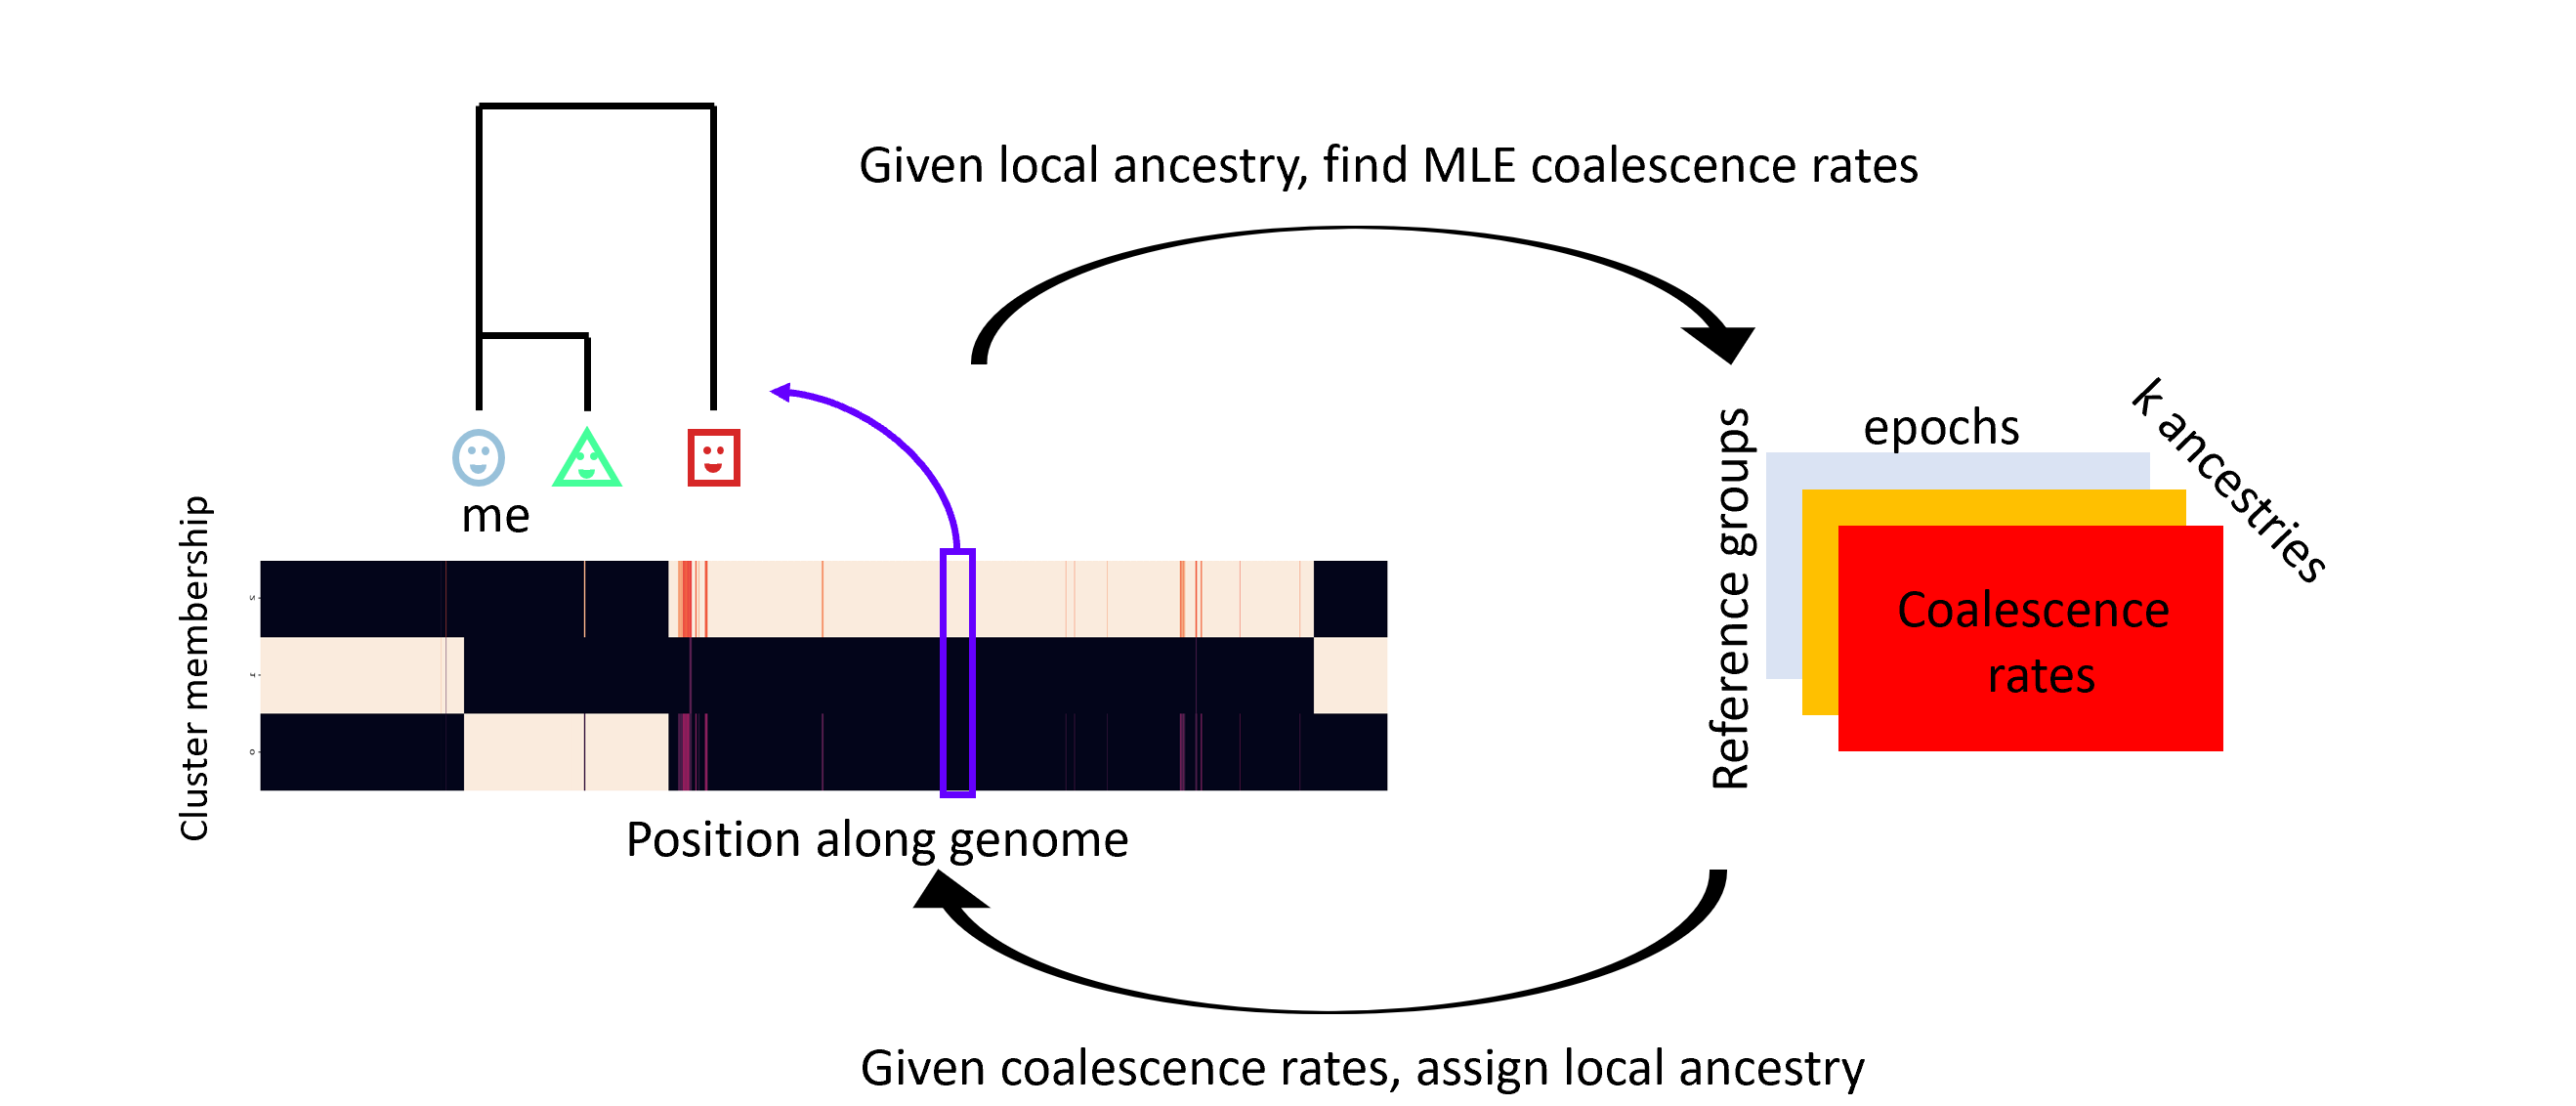
\includegraphics[scale=0.5]{figures/ghostbuster_method.PNG}
    \caption{\textbf{Overview of the GhostBuster algorithm.} The EM algorithm clusters the trees iteratively by successively updating the local ancestry given the coalescence rates in the E-step, and then the coalescence rates given the local ancestry in the M-step. }
    \label{fig:gb_overview}
\end{figure}


\subsection{PCA visualization to visualize ghost component}

To visualize the clustering of trees, we perform Principal Component Analysis (PCA) on the coalescence count and opportunity matrices obtained from the genealogies. The coalescence count matrix is an $N_{\text{ref}} \times N_{\text{tree}}$ matrix, where each entry $g,l$ represents the total contribution of reference group $g$ in the coalescence events at position $l$. In practice, we aggregate the contributions for all coalescence events occurring between predefined start and end time epochs, which typically correspond to the epochs used in the GhostBuster analysis. These epochs control the time periods in which we expect to observe differences in coalescence patterns. We construct a similar matrix for the opportunity, also an $N_{\text{ref}} \times N_{\text{tree}}$ matrix, where each entry $g,l$ records the total opportunity for reference group $g$ at position $l$. The same time epochs are used as in the coalescence count matrix to ensure consistency.

The coalescence count and opportunity matrices are then stacked to form a $2N_{\text{ref}} \times N_{\text{tree}}$ matrix, which is mean-centered and standardized. We perform eigen decomposition on this matrix to obtain the leading principal components. These principal components provide a visual interpretation of the clustering performed by GhostBuster, helping to better understand the patterns in coalescence across the genome.

\subsection{Coancestry curves to date admixture event}
\label{sec:ch2-gb-coancestry}

Given the local ancestry inferred using GhostBuster, we use coancestry curves to accurately estimate the date of the admixture event.
%
As described in section \ref{sec:ch1-gb-survey} the joint probability of observing ancestry a genetic distance `d' away is given as follows:
\begin{equation}
\begin{aligned}
    p_{AA}(g) &= \alpha ( e^{-g\lambda} + \alpha (1-e^{-g\lambda} )), \\
    p_{AB}(g) &= p_{BA}(g) = \alpha (1 - \alpha) (1 - e^{-g\lambda}), \\
    p_{BB}(g) &= (1-\alpha) ( e^{-g\lambda} + (1-\alpha) (1-e^{-g\lambda} ))
\end{aligned}
\end{equation}
where, $\alpha$ is the genome-wide proportion of ancestry `A' and $1-\alpha$ of ancestry `B'. 
%
We fit the exponential distribution to all possible ancestry combinations and jointly maximize the log-likelihood. 
%
In case of three or more way admixture we fit coancestry curves for each pair of ancestries at once, estimating the dates separately for each event.
%
We use block-jackknife across chromosomes to estimate standard errors with dating the admixture event.
% 
Additionally, we use diploid ancestry calls (summing the posteriors of two haplptypes) to avoid phasing errors to bias the admixture dating.

\subsection{Joint analysis of multiple targets}
Sometimes the reference populations can be themselves admixed. 
%
GhostBuster allows estimating the coalescence rates of the target lineage with reference populations conditioned on the local ancestry of the reference populations. 
%
It does so by counting coalescence events and opportunity separately for different ancestries in the admixed reference populations.  

It is also possible that the reference populations share the same admixture event as the target individual. To account for this, we employ a two-step procedure to fit the admixture event. First, we fit a mixture model assuming unadmixed reference populations, assigning ancestry to all admixed reference populations. Next, we threshold the inferred local ancestry probabilities for the reference populations and refit the mixture model conditioned on this local ancestry. This method allows for an approximate joint fitting of multiple target individuals.

\subsection{Tree Filtering}

We consider trees that are at least 10kb apart.
%
Additionally, for fitting the mixture model, we only retain trees which correspond to bottom 50\% of the recombination rates, where the recombination rate is calculated 500kb around the tree.
%
These trees usually have more mutations to support the tree topology and are therefore more accurate.
%
Additionally, we filter out regions corresponding to centromeres, telomeres, and the HLA region, along with a 500kb buffer around these areas. The positions of centromeres, telomeres, and the HLA region in the appropriate genome build were obtained from the \href{https://genome.ucsc.edu/goldenPath/help/ftp.html}{UCSC genome browser}.
%
Once the per-component coalescence rates and proportions are inferred we utilize them to infer the local ancestry of the whole genome including regions with high recombination rates.

\subsection{Choosing the number of components}
\label{sec:ch2-gb-selecting-clusters}

One of the critical decisions when decomposing local ancestry is selecting the appropriate number of components for our method. To determine the optimal number of components, we assess the log-likelihood on held-out chromosomes using a cross-validation approach, where one chromosome is left out at a time. The underlying assumption is that if the admixture is genuine, it should be replicated on a different chromosome.

The process is as follows: we first estimate the parameters (coalescence rates and proportions) using our EM algorithm on data from all avialable chromosomes except the held-out one. We then use the fitted parameters to evaluate the log-likelihood on the held-out chromosome. This procedure is repeated for multiple held-out chromosomes and varying numbers of components. Notably, the evaluation on the testing chromosomes is performed without the use of the HMM. The optimal number of clusters is determined by identifying the point at which the total log-likelihood on the held-out chromosomes is highest.

While this approach works well in simulations, real data presents additional challenges. The full admixture history of a sample is often complex, with the possibility that the source groups themselves are the result of earlier admixture events. Therefore, in practice, we choose the number of components based on how meaningfully we can interpret the components in the real data. In most cases, this leads to selecting two components. Overall, the exact choice of the number of components can be either data-driven, based on the held-out log-likelihood, or informed by prior knowledge about the admixture event.

\section{Data and quality control}
\label{sec:ch2-gb-data}
\subsection{Modern human datasets}

We work with multiple publicly available modern human datasets throughout our analysis, the datasets we analyze include the human genome diversity project (HGDP) \cite{cann2002human, bergstrom2020insights}, Simons genome diversity project (SGDP) \cite{mallick2016simons} and $1{,}000$ genomes project ($1{,}000$ GP) \cite{sudmant2015integrated, 10002015global}.
%
The whole-genome sequenced version of HGDP \cite{bergstrom2020insights} comprises of 929 individuals and 51 diverse population groups sampled across the globe with an average coverage of $34 \times$ (range: $23$-$75 \times$).
%
The 1,000GP dataset comprises 2,504 individuals, from 26 populations across the globe and an average coverage of $32 \times$ (range: $26$-$66 \times$).
%
The SGDP dataset comprises 278 individuals from 142 diverse populations across the globe and an average coverage of $43 \times$ (range: $34$-$83 \times$).

In particular, we use the unified version of HGDP and $1{,}000$ GP \cite{koenig2024harmonized}, where the genome from the two project were jointly called. 
%
We obtained the phased version of the dataset from \href{gs://gcp-public-data‐‐gnomad/resources/hgdp_1kg/phased_haplotypes_v2/}{here}. This dataset was called with hg38 genome build.
%
The phased data had already undergone variant QC to filter variants with (1) HWE $\geq 1 \times 10^{-30}$, (2) F\_MISSING $\leq 0.1$, or (3) ExcHet $\geq 0.5$ and ExcHet $\leq 1.5$. 
%
We additionally excluded multi-allelic SNPs and Indels from the dataset.
%
We also performed sample QC, by only retaining a subset of African samples from 1,000 GP (20 individuals per 6 African subgroups: `ACB', `ASW', `ESN', `LWK', `GWD', `MSL') and removing close relatives upto 2nd degree.
%
To remove relatives, we used the list of unrelated samples in HGDP+1,000GP inferred in the Allen ancient DNA resource \cite{mallick2024allen} and only retained individuals falling in this set.
%
Finally, we retained 45.6 million variants, and 1026 samples across 58 population groups in this dataset. 


The Simons Genome Diversity Project (SGDP) was called in hg37 genome build and was therefore not merged with the HGDP+1000GP dataset. 
%
We treated it separately as an independent validation dataset.
%
The phased data for SGDP was obtained from \href{https://sharehost.hms.harvard.edu/genetics/reich_lab/sgdp/phased_data.knownbugs.not_recommended.please_use_newer_dataset_instead/}{here}. 
%
Apart from the filtering done in \cite{mallick2016simons} we additionally excluded multi-allelic SNPs and Indels from our analysis. 
%
We retained 28.3 million variants, and 278 samples across 130 population groups in this dataset.

\subsection{High quality ancient DNA resources}

The assembly and quality control of ancient DNA dataset was performed by Dr. Leo Speidel, who is one of the co-authors on the paper.
%
Apart from the modern samples, we also consider 49 ancient DNA and 4 archaic DNA samples. These samples were all high coverage with a average coverage of $17.3\times$ (range: $10.3$-$65.1 \times$). The ancient and archaic DNA samples used in the analysis are tabulated in \ref{tab:gb_ancient_samples}.

The ancient DNA BAM files were processed using \texttt{bcftools mpileup} to generate variant calls, selecting only reads with a mapping quality of 20 or higher, a base quality of 20 or higher, and a minimum depth of coverage of 5.
%
The variant calls from the ancient DNA samples were then merged with the $1{,}000$ GP (downloaded from \href{https://ftp.1000genomes.ebi.ac.uk/vol1/ftp/release/20130502/}{here}) and phased using \texttt{shapeit4}. The phasing process involved first phasing variants observed in $1{,}000$ GP and then using the phasing as a scaffold to phase variants not observed in $1{,}000$ GP within the ancient dataset. We additionally randomly phased singletons in the ancient dataset. 
%
Subsequently, the ancient DNA dataset was lifted over to the hg38 reference genome using \texttt{picard LiftoverVcf} and merged with the unified version of HGDP+1000GP using the \texttt{bcftools merge -0} option. This merging resulted in only 22 bi-allelic SNPs (less than $0.001$\%) on chromosome 20 that were missing in one dataset but were common in other (allele frequency $\geq 0.25$). After merging, we filtered out multi-allelic variants, duplicate variants, and indels. As a final sanity check, we compared allele frequencies between the HGDP+1000GP dataset and the ancient DNA dataset, finding a high correlation with minimal missingness (see Figure \ref{fig:gb-sanity-check}).

\subsection{Building genome-wide genealogies for moderns and ancients}

We use Relate \cite{speidel2019method} to construct genealogies from phased data for both modern and ancient samples. For genealogies involving only modern samples, we apply a genomic mask provided with the HGDP or 1000 Genomes Project datasets, retaining only regions marked as "passing" to exclude variants with high uncertainty. Additionally, we mask sites where the human ancestral allele FASTA file (accessible \href{ftp://ftp.ensembl.org/pub/release-74/fasta/ancestral_alleles/homo_sapiens_ancestor_GRCh37_e71.tar.bz2}{here}) shows missing data, as well as sites corresponding to multi-allelic SNPs or indels. For genealogies that include ancient samples, we further refine this mask by considering only sites that pass in all Neanderthal and Denisovan masks (accessible \href{http://ftp.eva.mpg.de/neandertal/}{here}). Additionally, we filter out sites where other ancient samples exhibit more than 2\% missingness. The masks corresponding to ancient DNA are lifted over to the hg38 reference genome to ensure consistency.

To identify the most likely ancestral allele for each SNP, we use an estimate of the human ancestral genome. We utilize the HapMap3 inferred recombination rate maps for builds hg37 and hg38, which can be downloaded \href{https://github.com/odelaneau/shapeit5/tree/main/resources/maps/}{here}. The mutation rate is set to $1.25 \times 10^{-8}$ for building genealogies of modern samples, while for genealogies involving ancient samples, the mutation rate is adjusted to $4 \times 10^{-9}$, and only transversions are used to date the branch lengths. To ensure consistency in the genealogies, we enforce the construction of topologies every 10kb using the \texttt{--fb} option. When working with ancient samples, we provide the estimated ages of the samples to enhance the accuracy of the genealogies. The population size of the sample is estimated by iteratively fitting population sizes and branch lengths for chromosome 1 over five iterations. The converged population size is then used as a prior for dating branch lengths on the remaining chromosomes. Finally, the resulting trees are converted to tskit format for use with GhostBuster.

\section{Accurate local ancestry inference in simulations}
\label{sec:ch2-gb-sim}
\subsection{Simulation design}
\label{sec:ch2-gb-sim-design}

To assess the power and robustness of detecting ghost populations, we simulate two distinct admixture scenarios: a four-way recent admixture and Denisovan admixture into Papuans. For both simulations, we use a constant mutation rate of $1.25 \times 10^{-8}$ and the HapMap3 recombination rate map, excluding regions with zero recombination rate, centromeres, telomeres, and the HLA region on chromosome 6. We simulate the demography using msprime \cite{kelleher2016efficient}.

\begin{enumerate}
    \item \textbf{Four-way recent admixture:} In this scenario, we assume four reference populations (A, B, C, and D), each contributing 25\% to form the focal individual 5,000 years ago. Populations A and B split $50{,}000$ years ago, as did populations C and D, with all populations merging back together $100{,}000$ years ago (Figure \ref{fig:sim1}a). We assume a constant population size of $20,000$ for all populations after their split and $10{,}000$ for the super-populations prior to $50{,}000$ years ago. To assess the case without a ghost population, we sample 10 diploid individuals from each population and 1 focal (admixed) individual. For the ghost population scenario, we sample 10 individuals each from populations A, B, and C, with none from population D. 
    
    \item \textbf{Denisovan Introgression into Papuans:} This scenario uses the simulation model and script provided by \cite{skov2018detecting} to simulate Denisovan introgression into Papuans. We assume three reference populations (Papuans, Africans, and Denisovans), where Papuans and Africans split $72{,}036$ years ago, and Denisovans split from modern humans $656{,}908$ years ago (Figure \ref{fig:sim1}b). Denisovans admixed with Papuans around $43{,}935$ years ago with a 5\% admixture proportion. The population sizes are $3,899$ for modern Papuans, $27{,}122$ for Africans, and $4{,}947$ for Denisovans before they went extinct. We also simulate the Out-of-Africa bottleneck, where the Papuan population size drops upto $136$. A graphic overview of this simulation is shown in Figure \ref{fig:sim1}b. We fit five Papuan individuals, using 20 Papuans and 25 Africans as the reference panel. Additionally, we assess the power and compare local ancestry estimates with and without an ancient Denisovan sample dated to 67,570 years ago.    
\end{enumerate}

\begin{figure}
    \centering
    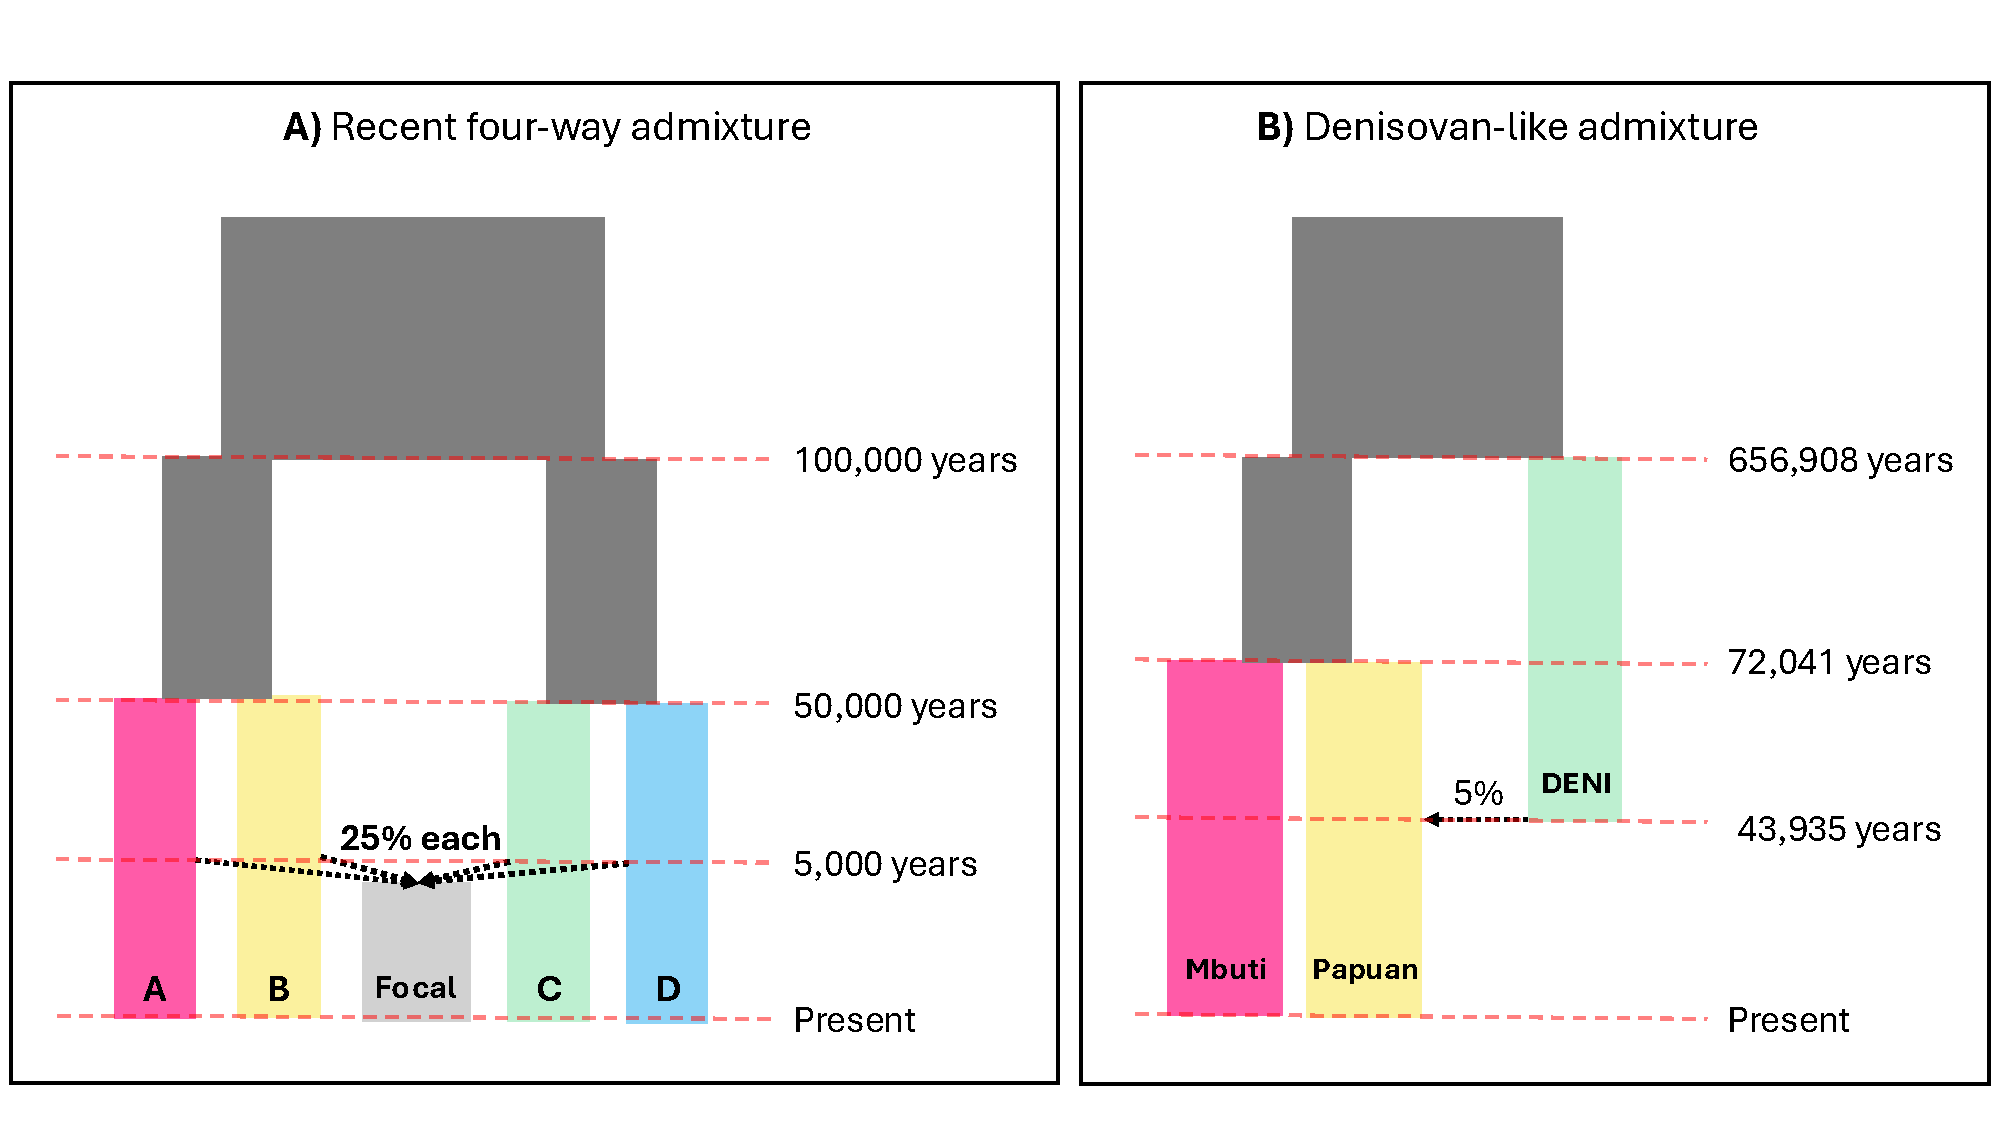
\includegraphics[width=\textwidth]{figures/thesis_gb_sim_design.pdf}
    \caption{\textbf{Simulation design for performance evaluation.} A. Four-way recent admixture simulation, B. Simulated Neanderthal introgression into Han Chinese. The simulation parameters including the population size, mutation rate and recombination map are described in section \ref{sec:ch2-gb-sim-design}.}
    \label{fig:sim1}
\end{figure}

\subsection{Four-way recent admixture}

%% para 1
% How many individuals we simulate, whats the target, whats the reference? 
% number of chromosomes? 
% We expect a 4-way admixture (see simulation design section)
% We run the method on both true trees and relate trees inferred using the variation data

We validated GhostBuster's ability to detect admixture events through a simple simulation, where we modeled a recent 4-way admixture event occurring 5,000 years ago, involving groups that had been separated for at least 50,000 years (see Figure \ref{fig:sim1}a). The focal individual in our simulation resulted from an equal contribution of 25\% ancestry from four distinct reference populations, labeled A, B, C, and D. We sampled up to 10 individuals from each reference population and used chromosomes 1 through 5. More details about the simulation setup can be found in Section \ref{sec:ch2-gb-sim-design}. Our objective was to decompose the focal individual's ancestry both with and without access to all reference populations, with the expectation of accurately identifying the four ancestral components. We applied our method primarily to trees inferred using genetic variation data via Relate, assuming a constant mutation rate of $1.25 \times 10^{-8}$, while results comparing with true trees simulated using msprime are also presented. Additionally, we only focused on coalescence events occurring from 0 to 50,000 years.

%% para 2
% We first tested the method with k=4 and presence of all reference groups
% We started with random init. and EM for 200 iterarions
% We found the four-components coal. rates represented four-populations (1 - a, 2 -b, ..)
% The coal. rates are more distinct and seperated for true trees than relate trees, representing the error in building genealogies 
% In order to compute the accuracy, we compared local ancestry with the true local ancestry R2 = 
% Calibration plots

We first tested the method with access to all four reference populations. We applied our approach to decompose the focal individual's ancestry into four components or clusters. Starting with a random initialization of coalescence rates and proportions, we fit our model over 200 EM iterations until the log-likelihood converged. The converged inverse coalescence rates represent the four clusters that maximally distinguished the coalescence events for the focal individual (see Figure xx). The inverse coalescence rate (ICR) for each component can be interpreted as the component's affinity toward one of the four reference populations—a lower ICR value indicates quicker coalescence with that specific reference population. Our analysis revealed that the four clusters identified by GhostBuster contributed roughly 25\% to the focal individual's ancestry, with each cluster closer to one of the four reference populations. For instance, component 1 was closest to population A, component 2 to population C, component 3 to population B, and component 4 to population D. When applied to true simulated trees (see Figure app1), the coalescence rates were more distinct and better separated, highlighting the fuzziness in building genealogies from genetic variation data. To assess the accuracy of our decomposition, we compared the local ancestry inferred by our EM algorithm with the simulated ground truth local ancestry. We observed a strong correlation between the local ancestry posterior inferred by GhostBuster and the ground truth, with an $R^2$ of $0.99$. Finally, we evaluated the calibration of our local ancestry estimates and found them to be well-calibrated, with an expected calibration error (ECE) of $121$ (see Figure yy).

%% para 3
% Next we removed population D from reference
% We did similar procedure with k = 4 
% four components, with the fourth component being distant from all 3 sampled reference populations
% local ancestry R2
% calibration plots

Next, we removed population D (without loss of generality) from the genealogies and attempted to decompose the focal individual. This scenario simulates the presence of a ghost population, as population D contributed to the focal individual's genetic makeup but is not included in the reference panel. We reran our method, fixing the number of components to four. The four components still contributed roughly 25\% to the total ancestry. The inverse coalescence rates (ICRs) for each component only existed for populations A, B, and C, as no individuals from population D were sampled. Component 1's ICR was closest to population A, component 2 was closest to population B, and component 3 was closest to population C (see Figure xx). However, component 4 was more distantly related to all three populations, indicating slower coalescence with each. This could be the ancestry relating to population D which could have been tagged by its slower coalescence rates with populations A-C (see Figure xx). To verify this, we compared the local ancestry inferred by running our EM algorithm without the access to population D with the simulated ground truth. We found a strong correlation, with an $R^2$ value of 0.98, indicating that component 4 effectively captured the ancestry related to population D without requiring direct samples from that population. A visual comparison of the local ancestry inferred using Relate trees, both with and without the inclusion of reference population D, is shown in Figure zz. Finally, we assessed the calibration of our local ancestry estimates in this setting and found them to be well-calibrated, with an expected calibration error (ECE) of 121 (see Figure yy).

%% para 4
% How do we choose number of components? 
% held-out validation 

We performed leave-one-chromosome-out cross-validation to determine the optimal number of components, as described in Section \ref{sec:ch2-gb-selecting-clusters}. We found that four components provided the best fit in both scenarios, whether population D was present or absent (see Figure xx).

\subsection{Denisovan-like Introgression into Papuans}

%% explain the simulation
%% with denisovan
%% without denisovan
%% comparison with skov 
%% add ablations on hmm vs no hmm, 

We examined the archaic introgression of Denisovan ancestry in modern-day Papuans by simulating an admixture event that occurred approximately 44,000 years ago, with an admixture proportion of 5\% (see Figure \ref{fig:sim1}b). The simulation parameters are from \cite{skov2018detecting}, and further details can be found in section \ref{sec:ch2-gb-sim-design}. For our analysis, we simulated 25 Papuan individuals, 25 Mbuti individuals (representing African ancestry), and a Denisovan ancient sample. We focused on chromosomes 1 through 5 for our analysis. Our objective was to decompose the Papuan individuals' ancestry both with and without access to the Denisovan sample, aiming to accurately identify Denisovan segments and admixture within Papuans. Similar to our previous simulation of a four-way recent admixture, we primarily applied our method to trees inferred from genetic variation data via Relate, assuming a constant mutation rate of $1.25 \times 10^{-8}$. Finally, we only focused on coalescence events occurring from 10,000 to 1,000,000 years for this analysis.

We begin our analysis by assuming we have access to one ancient Denisovan sample. We decompose five out of the 25 Papuan individuals, assuming two distinct components. As with the previous simulation, we randomly initialize the parameters and fit the EM algorithm for 200 iterations until the log-likelihood converges. The converged components reveal a major component, contributing around 95\% to the local ancestry, and a minor component contributing 5\% (see Figure xx). The inverse coalescence rates (ICRs) characterizing these components differ significantly. Component 1 demonstrates a slower coalescence rate with the ancient Denisovan sample and a relatively faster coalescence with the modern Mbuti samples. In contrast, component 2 exhibits a very fast coalescence with Denisovans but slower coalescence with modern Mbuti and Papuan samples. It is important to note that the most striking difference between the two components is the vastly accelerated coalescence with Denisovans in the minority group—up to over $1{,}000 \times$ faster compared to the majority group. However, there is also a substantial difference in coalescence with modern groups, which we will leverage to decompose the ancestry without access to the ancient Denisovan sample.

\begin{figure}[h!]
    \centering
    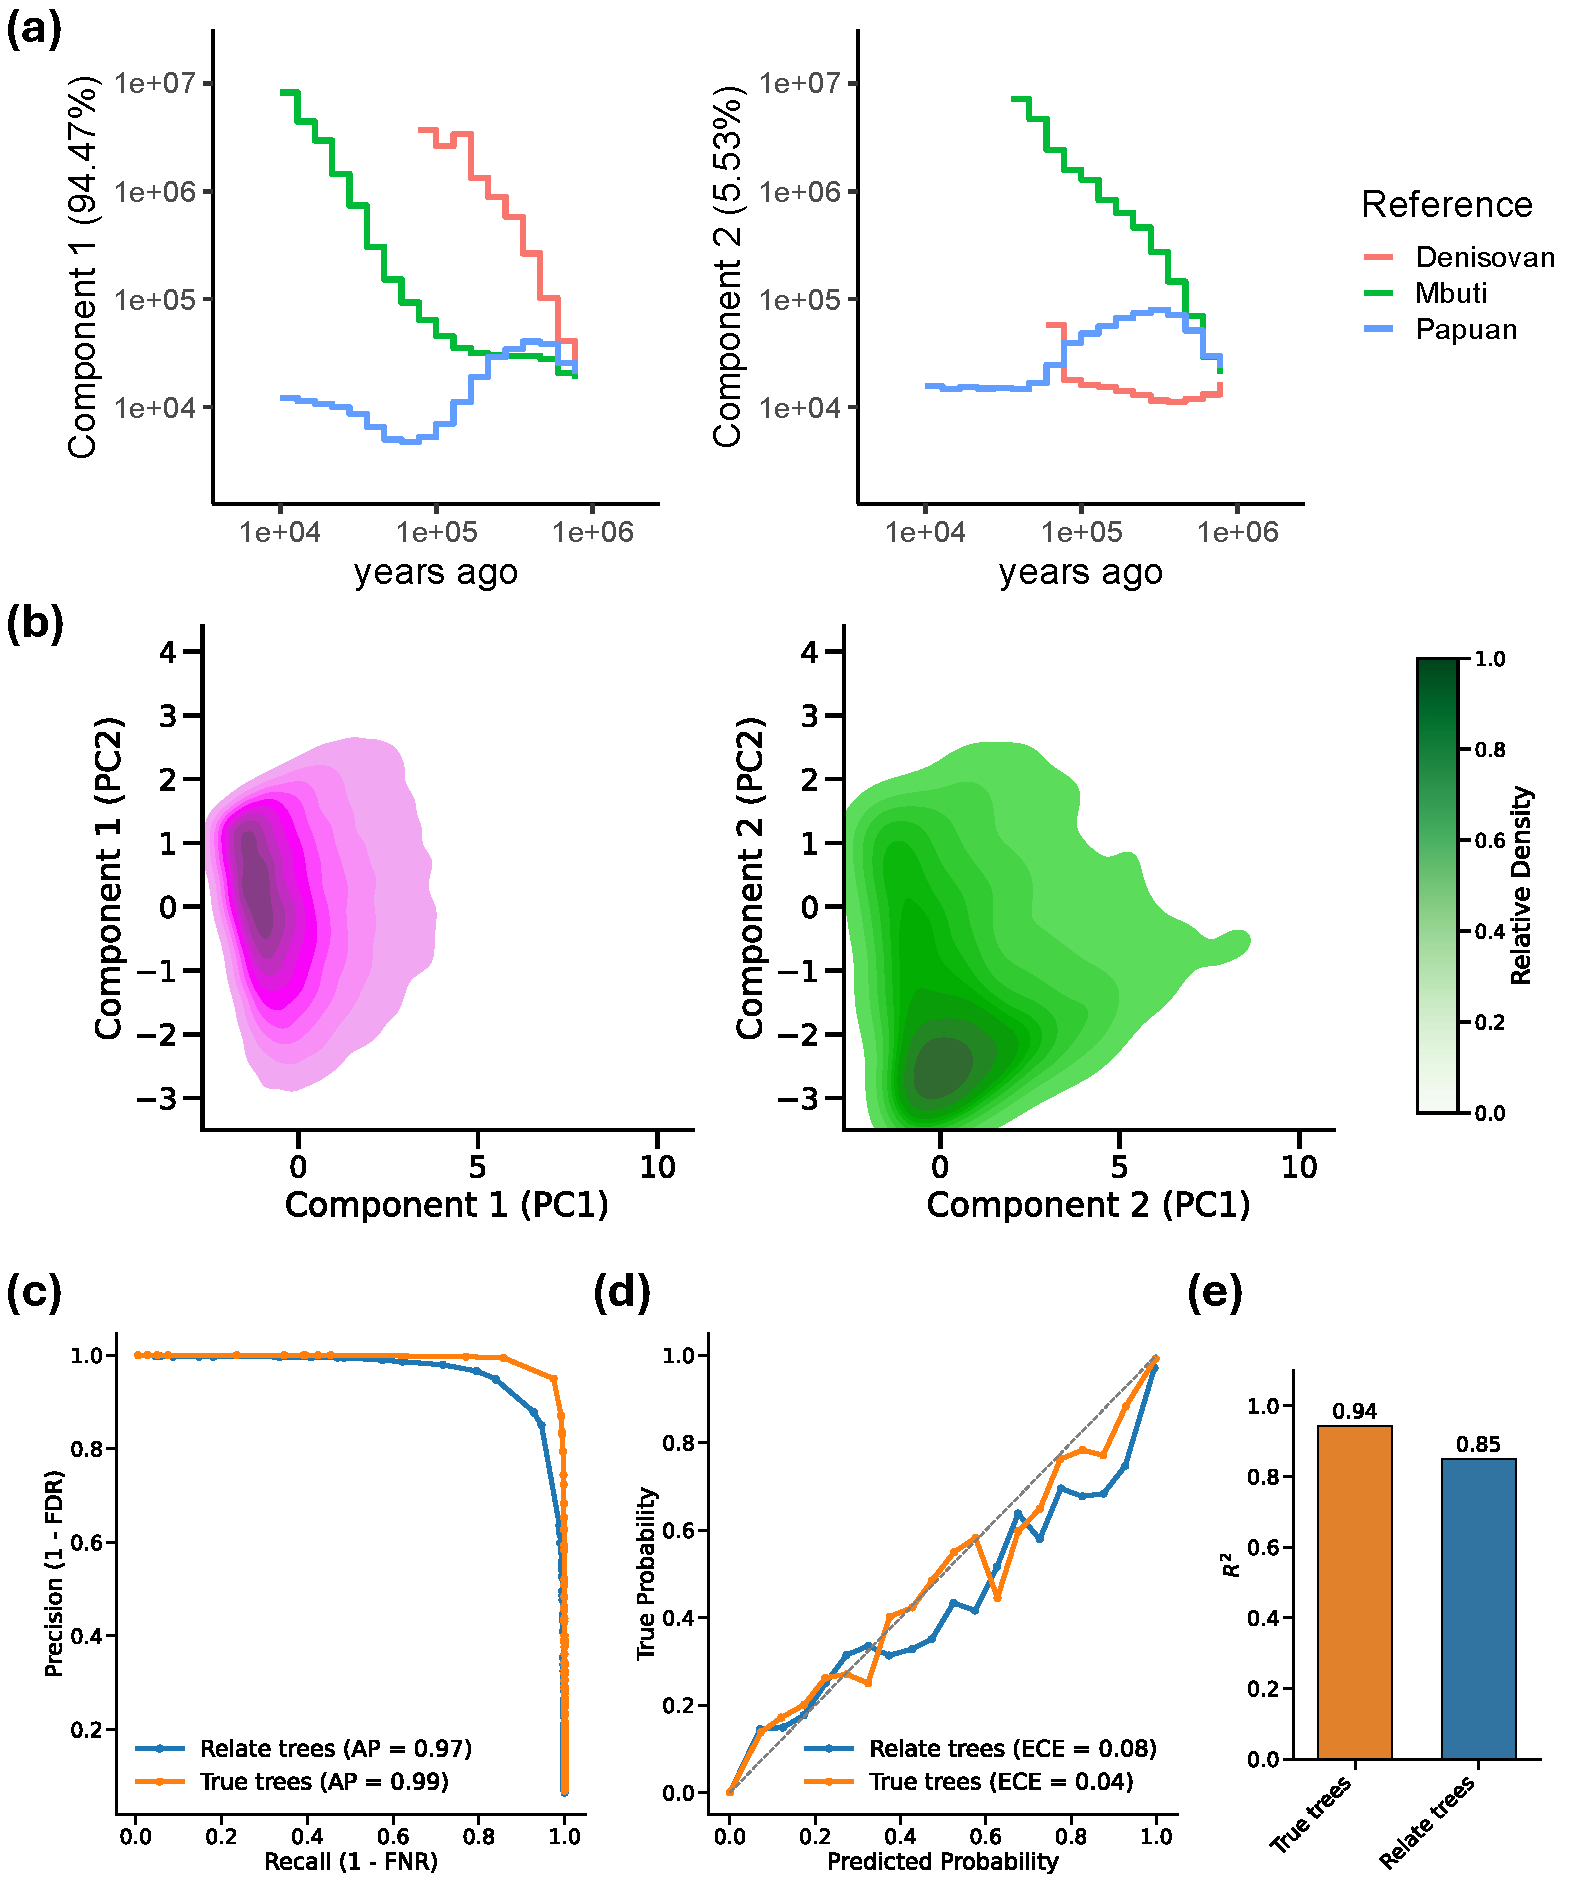
\includegraphics[width=\linewidth]{figures/gb_sims/thesis_gb_sim_denisovan_relate_ghost.pdf}
    \caption{
    \textbf{Decomposing Papuan individuals in simulations with Mbuti and Denisovans as additional references.} (a) Inferred inverse coalescence rates and proportions: each line represents inverse coalescence rate profiles with a reference population. (b) PCA visualization of the coalescence count and opportunity matrix derived from the genealogies plotted separately for each component. (c) Precision-recall curves, (d) Calibration curves, and (e) Prediction $R^2$ for inferred local ancestry compared to the simulated ground truth, where inference was done using true trees or Relate trees. The PCA visualization in (b) is based on a KDE plot with a threshold of 0.05, and binary local ancestry estimates are obtained by thresholding the inferred posteriors at 0.5.
    }
    \label{fig:enter-label}
\end{figure}

Next, we removed the Denisovan samples from our analysis and decomposed the same Papuan individuals into two components. In this scenario, the Denisovan ancestry in Papuans can be thought of as ghost population. Our method converged on two components, contributing approximately 95\% and 5\% to the local ancestry, respectively (see Figure xx). The ICRs of the minor component closely matched those of the minor component from the earlier analysis that included the Denisovan sample, showing slower coalescence with Mbuti and Papuans. Similarly, the major component demonstrated relatively faster coalescence with Mbuti and other Papuans. To verify that the minor component indeed represents Denisovan ancestry, we compared the local ancestry inferred using GhostBuster with the simulated ground-truth local ancestry. Additionally, we compared local ancestry inferences between true trees and Relate trees, both with and without access to the Denisovan sample. Our method outperformed a recent HMM-based approach tailored for detecting archaic introgression in non-Africans, yielding a higher $R^2$ value. Finally, we assessed the calibration of our local ancestry estimates and found them to be well-calibrated as shown in Figure zz.

We performed leave-one-chromosome-out cross-validation to determine the optimal number of components, as described in Section \ref{sec:ch2-gb-selecting-clusters}. We found that two components provided the best fit in both scenarios, whether Denisovan was present or absent (see Figure xx). Additionally, to test the robustness of our method, we also attempted to decompose Mbuti individuals in the same simulation, which are panmictic with no simulated population structure or admixture. We found that the likelihood corresponding to a single component outperformed the others, suggesting no admixture or significant coalescence differences among clusters.

\section{Identifying several recent admixtures accurately}
\label{sec:ch2-gb-real}

Haplotype-based methods like Alder \cite{loh2013inferring}, Globetrotter \cite{hellenthal2014genetic}, and Mosaic \cite{salter2019fine} have been instrumental in confidently inferring recent admixture events, particularly those occurring less than 1,500 years ago. We focus on several well-documented, recently admixed populations from the Human Genome Diversity Project (HGDP), including the Hazara, Bedouin, Maya, and Sindhi. Each of these populations has undergone 2- or 3-way admixture events within the past few thousand years, which have been reliably detected by previous methods. Our objective is to decompose the ancestry of individuals from these populations using GhostBuster and to compare the local ancestry with results from other haplotype-based methods.

We begin by decomposing the ancestry of Hazara individuals from the HGDP, who have been shown in previous studies to result from recent admixture between groups similar to modern-day Pathans and Mongols \cite{hellenthal2014genetic,salter2019fine}. Using all populations in our HGDP+1,000GPA dataset (as described in section \ref{sec:ch2-gb-data}), we fit two components to decompose the genome-wide ancestry of the 21 Hazara individuals. We focused on coalescence events within the last 50,000 years, dividing the time scale into 20 logarithmically spaced epochs ranging from 500 to 50,000 years. Our analysis revealed that the Hazara individuals could be decomposed into two components, each contributing roughly 50\% to the overall ancestry. The inverse coalescence rates (ICRs) indicate that component 1 is closely related to East Asian groups such as Mongols and others, while component 2 is more closely aligned with South Asian groups like the Pathans—consistent with previous findings using ChromoPainter (see Figure yy). To further validate our results, we compared the local ancestry estimates from our method with those obtained using Mosaic, which was run using all reference populations in HGDP. We found that the local ancestry was highly correlated between the two methods, with an $R^2$ of 0.92. Potential differences in local ancestry estimates may be attributed to additional steps in Mosaic, such as correction for phasing, which are not present in our method. Additionally, when we excluded South Asian samples from the reference panel, we still identified similar components with comparable local ancestry inference, though the correlation with Mosaic decreased ($R^2 = 0.61$, see Figure xx). 

We conducted similar analyses for other populations in the HGDP, including the Bedouin (with European and African admixture), Maya (with African, Native American, and European admixture), and the Sindhi and Druze populations (both of which exhibit East Asian and South Asian admixture). The proportions of admixture, potential source populations, and estimated timing of these admixture events for each population are summarized in Table xx. A more detailed analysis for each population, along with visual representations, can be found in the appendix (see Figures xx, yy, zz, and aa).
\chapter{\label{ch:3-gb-result}Understanding population structure in Africa using GhostBuster}

\minitoc

\section{Chapter overview}

In this chapter, we utilize GhostBuster to analyze real genetic data from various publicly available modern and ancient human datasets to gain insights into the evolutionary history of humans in Africa. 

In Section \ref{sec:ch3-lit-review}, we start by providing an overview of previous population genetics research that has contributed to our understanding of both recent and ancient history in Africa.
%
In Section \ref{sec:ch3-gb-bta}, we uncover evidence of Eurasian-like ancestry within African populations using GhostBuster. Our analysis identifies two distinct sources for this ancestry: repeated back-migration events from Eurasia over the past $10{,}000$ years and a deeper event more than $15{,}000$ years ago involving a population that likely remained in Africa but shares a close genetic relationship with populations outside Africa. 
%
In the remainder of the section, we characterize the back-to-Africa event and present independent strategies to validate it. These include estimating the timing of the admixture, identifying likely source populations, analyzing correlations with Neanderthal ancestry in African populations, and investigating population-specific mutational signatures.
%
In Section \ref{sec:ch3-gb-deep}, we investigate the older admixture event involving early interactions between populations that differentially relate with the out-of-Africa lineage. 
%
We propose several validation strategies for this ancient event, including distinguishing it from recent back-to-Africa migrations by the absence of Neanderthal ancestry, leveraging GC-biased mutational signatures at recombination hotspots, and demonstrating higher trait predictability in segments corresponding to the component closely related to out-of-Africa groups.
%
Finally, in Section \ref{sec:ch3-discussion}, we conclude the chapter by synthesizing the key findings from applying GhostBuster to both simulations and real data, and we outline potential directions for future research.


\section{Overview of African population history}
\label{sec:ch3-lit-review}

Africa is widely recognized as the cradle of modern humans, with fossil evidence of Homo sapiens dating back approximately $300{,}000$ years \cite{day1969early,hublin2017new,bergstrom2021origins}. This view is further supported by population genetics data, which reveal Africa’s extraordinary genetic diversity -- more than twice that of any other continent \cite{yu2002larger} -- and some of the oldest population splits in human history. Despite Africa's crucial role in human genetics, unraveling its population history poses significant challenges. The preservation of ancient DNA is hindered by the region’s hot and humid climate, resulting in a scarcity of ancient genetic samples. Additionally, recent demographic events, including back-to-Africa migrations, the Bantu expansion \cite{tishkoff2009genetic}, and European colonization, have obscured ancient genetic signals in modern samples, complicating efforts to reconstruct Africa's deeper genetic history.

In this section, we provide an overview of population genetics advancements in understanding the continent’s population history. We begin with relatively recent events, such as European colonization, maritime trade, and the Bantu expansion in Section \ref{sec:ch3-bantu-europe}, then explore older back-to-Africa migrations in Section \ref{sec:ch3-back-to-africa}, and finally delve into the deep population structure that characterizes Africa’s genetic landscape in Section \ref{sec:ch3-deep-population-structure}.

\subsection{Colonization, maritime trade and Bantu expansion}
\label{sec:ch3-bantu-europe}

Africa has experienced significant demographic changes in the recent past. Among the most recent ones were the ones due to European colonization and the trans-Atlantic slave trade in the last five hundred years. The trans-Atlantic slave trade forcibly displaced millions of Africans, primarily from West Africa to the Americas. Many died en route, while others survived and admixed with Indigenous Americans and Europeans \cite{micheletti2020genetic}. Within Africa, the genetic impact of European colonization was more limited due to sociopolitical barriers, segregation policies, and cultural divisions \cite{tishkoff2009genetic}. Nonetheless, some localized admixture occurred between Europeans and Africans, particularly in regions around trade ports and settler colonies, such as South Africa.

The maritime trade and Indian Ocean trading network over the past two thousand years have profoundly influenced the genetic diversity and cultural heritage of African populations. One striking example is the Malagasy people of Madagascar, who speak an Austronesian language -- remarkably different from other African languages. Several studies, including Pierron et al. \cite{pierron2014genome, pierron2017genomic}, provide evidence that the genetic composition of present-day Malagasy populations reflects a significant admixture event involving East African Bantu-speaking populations and Southeast Asians. This admixture is thought to have occurred in the first millennium CE, facilitated by the Indian Ocean trading system, which brought Austronesian-speaking seafarers from the Indonesian archipelago (approximately $7{,}500$ kilometers away) to Madagascar. These Southeast Asian seafarers carried with them their language, agricultural techniques, and cultural practices, which later blended with those of East African populations, creating the unique genetic and cultural identity of the Malagasy people. 

Apart from Madagascar, maritime trade profoundly influenced several coastal regions in eastern Africa. Notably, the Swahili coast -- which includes parts of modern-day Kenya, Tanzania, and Mozambique, as well as the islands of Zanzibar, Pemba, and the Comoros, was significantly shaped by the Indian Ocean trade network. Brielle et al. \cite{brielle2023entwined} utilized ancient DNA from the Swahili coast to demonstrate that these extensive trade routes, connecting Africa with the Middle East, South Asia, and Europe, facilitated not only the exchange of goods but also the movement of people. This movement resulted in gene flow between African populations and traders from distant regions. Their study uncovered substantial Persian and Arab ancestry among both ancient and present-day individuals from the Swahili coast.

The Bantu expansion predates the maritime migrations and colonization of Africa and is recognized as one of the largest and most impactful migrations in African history. Bantu is one among over $500$ closely related languages within the Niger-Congo language family, collectively spoken by more than $300$ million people today, across an expanse of roughly $5{,}000{,}000$ square kilometers. Several population genetic studies \cite{tishkoff2009genetic,de2012bringing,li2014genetic,patin2017dispersals,fortes2024genetic} have shown the Bantu-expansion not only led to spread of the language but was also accompanied by population movement and advent of farming in Africa. The expansion is believed to be have started $4{,}000$ to $6{,}000$ years ago from West Africa and eventually spread to East and then South Africa. There is still considerable debate about the exact migration paths chosen during the expansion, but nonetheless the Bantu expansion led to wide-spread mixing or replacement of local hunter gatherer and pastoralist groups across Africa. 


\subsection{Back-to-Africa migration}
\label{sec:ch3-back-to-africa}


Migrations from Eurasia into Africa have been identified before. 
%
North African groups such as the Mozabites, Moroccans, Tunisians, and Egyptians are primarily descended from ancient inhabitants of North Africa, who have been part of the West Eurasian clade for over $10{,}000$ years. Additionally, the Arab slave trade introduced some sub-Saharan African ancestry into these populations within the last millennium \cite{price2009sensitive, hellenthal2014genetic, salter2019fine}.
%
One of the primary barriers to migration into Africa is the vast Sahara Desert, which would have impacted migrations from Eurasia into sub-Saharan Africa.
%
However, it is well known that the Sahara underwent periodic climate cycles due to changes in Earth's orbit, transitioning between arid and humid phases. 
%
The humid phase, often referred to as the ``Green Sahara'' period, could have made migrations into and out of Africa more feasible. The last Green Sahara period occurred approximately $5{,}000$ to $11{,}000$ years ago \cite{tierney2017rainfall, larrasoana2013dynamics}.

One of the first studies to identify potential Eurasian ancestry in sub-Saharan Africans was conducted by Pickrell et al. \cite{pickrell2012genetic, pickrell2014ancient}. The authors utilized ALDER \cite{loh2013inferring}, a method designed to identify and date admixture signals through coancestry curves (as described in Section \ref{sec:ch2-gb-coancestry}), and found evidence of West Eurasian ancestry in South and East African populations, but not in West or Central Africans. The estimated proportions of West Eurasian ancestry were up to 14\% in South African populations and up to 50\% in East African populations. The admixture events were dated to approximately $900$--$1{,}800$ years ago in South Africa and $2{,}700$--$3{,}300$ years ago in East Africa. Furthermore, the study revealed that the Eurasian ancestry in both South and East Africa was shared, leading to the theory that the most likely source of Eurasian ancestry in South Africa originated from East Africa. While the findings strongly supported a ``back-to-Africa'' migration event, the method’s limited statistical power and reliance on reference populations may have hindered the detection of similar events in other African populations. These populations may have experienced smaller proportions of Eurasian ancestry or older admixture events, which were beyond the resolution of the study.

In another study, Llorente et al. \cite{llorente2015ancient, noauthor_2016-cy} sequenced an ancient individual from the Mota caves in Ethiopia, who lived approximately $4{,}500$ years ago. This ancient DNA sample provided direct evidence of Eurasian ancestry in African populations, as it was considered to predate the back-to-Africa migration event and thus served as a reference population without any Eurasian admixture. Using the Mota individual as a reference, the study identified 4 to 7\% West Eurasian ancestry in East African populations, with lower proportions observed in some southern African populations. However, this analysis relied on a reference out-group population and summary statistics derived from allele frequency differences, which tend to be underpowered for detecting subtle admixture signals.


Several studies have identified small amounts of Neanderthal ancestry in African individuals, suggesting a back-to-Africa migration as a plausible explanation \cite{chen2020identifying,vernot2016excavating}. 
%
Chen et al. \cite{chen2020identifying} developed a novel method called IBDmix to detect introgressed Neanderthal sequences in African individuals. The authors discovered that per individual, modern-day Africans carry between 16.4 and 18 megabases (Mb) of Neanderthal sequence per individual, which is roughly one-third of the Neanderthal sequence found in modern-day non-Africans. 
%
Interestingly, 94\% of the Neanderthal sequences identified in African samples were shared with non-Africans, with a significantly higher overlap observed with Neanderthal sequences found in Europeans compared to East Asians.
%
To explain the large amount of Neanderthal ancestry that they identify, combined with very short tract lengths, the authors propose a model involving an ancient migration of humans to Neanderthal regions, followed by a more recent back migration to Africa, as the most likely explanation for the presence of Neanderthal segments in African populations.
%
Overall, the study provides independent validation of a backflow event into Africa, though it does not have the resolution to precisely characterize the proportions and timings of this event.

Finally, ancient DNA from North Africa has revealed significant ancient migrations from the Middle East and Europe into the African continent \cite{van2018pleistocene, fregel2018ancient, simoes2023northwest}.
%
The Taforalt individual, sequenced from eastern Morocco and dated to $15{,}000$ years ago, exhibited genetic composition that was two-thirds similar to Middle Eastern hunter-gatherers and one-third similar to sub-Saharan Africans \cite{van2018pleistocene}.
%
Recent studies have uncovered additional ancient DNA in North Africa, indicating not only migrants from the Middle East but also European Neolithic farmers who introduced new lifestyles to North Africa between $7{,}000$ and $9{,}000$ years ago \cite{fregel2018ancient, simoes2023northwest}. 
%
These migrations from the Middle East and Europe likely influenced the genetics of populations in regions north of the Sahara. However, the extent to which such migrations impacted populations south of the Sahara remains an open question, given the Sahara’s historical role as a barrier to large-scale gene flow.

\subsection{Deep population structure within Africa}
\label{sec:ch3-deep-population-structure}

The population structure in Africa prior to the Out-of-Africa event has been a topic of considerable debate, with compelling evidence supporting the existence of structured populations even before humans expanded out of Africa.
%
Scerri et al. \cite{scerri2019beyond} argue that fossil data from Africa do not reflect contemporary humans emerging progressively in a single region. Instead, these fossils suggest that humans appeared at different times and in various combinations, exhibiting diverse ancestral features. This perspective is supported by findings suggesting that modern human cognition may have developed independently in multiple regions, alongside paleo-climatic models that reveal how periodic climate fluctuations likely influenced migration and adaptation \cite{mcbrearty2000revolution,demenocal2011climate}.
%
The structured African metapopulation model proposed by Scerri et al. challenges the simple tree-like model of human evolution. This model suggests that ancient populations could coalesce, split, experience gene flow, or go extinct over time. Scerri et al. found that the structured metapopulation model, also referred to as the ``population fragmentation and coalescence model'', better explains the genetic and archaeological data compared to a simple panmixia model, which assumes a single, interbreeding population.

There has also been considerable research showing evidence for unsampled or ``ghost'' archaic hominids in Africa \cite{skoglund2017reconstructing,ragsdale2019models,hammer2011genetic,lorente2019whole,durvasula2020recovering}. For instance, Durvasula et al. utilized the conditional site frequency spectrum (CSFS) to identify an archaic component in West Africans that diverged from modern humans over $700{,}000$ years ago and contributed up to 19\% to the genetic makeup of contemporary West African populations. Similarly, the Relate study reported an excess of long genetic branches in Africa, akin to patterns of Neanderthal ancestry in Europe \cite{speidel2019method}. Despite these studies, archaic introgression in Africa is still debated as methods struggle to account for the possibly complex population structure in Africa.
%
% Despite these debates, African populations exhibit far more long genetic branches than non-African populations, with an average of $42{,}434$ mutations unique to Africans compared to $7{,}012$ in non-Africans. This suggests more complex population dynamics, either due to archaic introgression or isolation by distance \cite{speidel2019method}.

Hollfelder et al. \cite{hollfelder2021deep} and Ragsdale et al. \cite{ragsdale2023weakly} argue that the model of archaic admixture in Africa does not fully explain the genetic diversity of present-day African populations. Ragsdale et al. applied a maximum likelihood framework to infer demographic parameters that best explain the one- and two-locus statistics for various African groups. The authors found that the ``population fragmentation and coalescence model'' \cite{scerri2019beyond} consistently outperformed other models, including those involving archaic admixture in Africa. The model proposed by Ragsdale et al. describes a weakly structured stem, with three co-existing stem populations more than $100{,}000$ years ago. These populations underwent migration among themselves and eventually merged in different proportions to form present-day African populations. The proposed model aligns more closely with the archaeological data from that period but remains limited by model misspecification, as it imposes constraints on the range of possible models when inferring demographic parameters.

Ancient DNA in Africa is scarce due to poor preservation in hot and humid conditions, but there are a few samples spanning the past $18{,}000$ years. Lipson et al. \cite{lipson2022ancient} argue that analyzing these ancient samples helps reduce confounding factors from more recent events such as back-to-Africa migrations, the Bantu expansion, and European colonization. By studying the ancient DNA of 31 samples, the study aimed to understand the population structure of hunter-gatherers in central and southern Africa, which represent some of the deepest splits in modern human lineages. Using supervised PCA, the researchers categorized the ancient samples based on three modern African groups: the San from southern Africa, the Mbuti from central Africa, and the Dinka from northeastern Africa. The authors found increasing regionalization among the ancient samples, with genetic similarities best predicted by geographic locations, suggesting minimal long-range migrations within these groups. The observed patterns of variation in the ancient samples were best explained by admixture involving at least three ancestries between $20{,}000$ and $50{,}000$ years ago.

Finally, Cousins et al. \cite{cousins2024structured} provide statistical evidence for archaic admixture events that potentially affected all human populations. The study proposes a novel method based on the pairwise sequentially Markovian coalescent (PSMC \cite{li2011inference}) to identify events of population splits and mergers. Their analysis suggests that human populations underwent an admixture event approximately $300{,}000$ years ago with two deeply divergent human species, which diverged around 1.5 million years ago. The admixture proportions in all analyzed human populations were roughly 80:20.

\section{Evidence for widespread back-to-Africa migration}
\label{sec:ch3-gb-bta}

To investigate the admixture history within Africa, we used GhostBuster to analyze genetic data from 17 modern sub-Saharan African groups from the Human Genome Diversity Project (HGDP), the $1{,}000$ Genomes Project ($1{,}000$ GP), and Simon's Genome Diversity Project (SGDP). In addition, we examined five ancient African samples (coverage between $10.52$ - $18.51$), including a ~$7{,}900$-year-old sample from Shum Laka in Cameroon \cite{lipson2020ancient}; ~$1{,}900$- and $400$-year-old samples from Ballito Bay, Eland Cave, and Newcastle in South Africa \cite{schlebusch2017southern}; and a ~$4{,}500$-year-old sample from Mota Cave in Ethiopia \cite{llorente2015ancient}. The groups we analyzed are listed in Table \ref{tab:african_populations}, and a map of the geographic locations of all modern and ancient samples is provided in Figure \ref{fig:gb_bta_1}c.

\begin{table}[h!]
\centering
\begin{subtable}{\textwidth}
\centering
\resizebox{\textwidth}{!}{
\begin{tabular}{|l|l|l|c|}
\hline
\textbf{Population} & \textbf{Dataset} & \textbf{Location} & \textbf{Samples} \\ \hline
Esan & $1{,}000$GP & Nigeria & 20 \\ \hline
Gambian & $1{,}000$GP & Gambia & 20 \\ \hline
Luhya & $1{,}000$GP & Kenya & 20 \\ \hline
Mende & $1{,}000$GP & Sierra Leone & 20 \\ \hline
Biaka & HGDP & Central African Republic & 22 \\ \hline
Mandenka & HGDP & Senegal & 21 \\ \hline
Mbuti & HGDP & Democratic Republic of Congo & 12 \\ \hline
San & HGDP & Namibia and South Africa & 6 \\ \hline
Yoruba & HGDP & Nigeria & 21 \\ \hline
Bantu Kenya & HGDP & Kenya & 11 \\ \hline
Bantu SouthAfrica & HGDP & Botswana or Namibia & 8 \\ \hline
Somali & SGDP & Kenya & 1 \\ \hline
Luo & SGDP & Kenya & 2 \\ \hline
Masai & SGDP & Kenya & 2 \\ \hline
Ju Hoan North & SGDP & Namibia & 4 \\ \hline
Dinka & SGDP & Sudan & 3 \\ \hline
Khomani San & SGDP & South Africa & 2 \\ \hline
\multicolumn{3}{|l|}{\textbf{Total}} & \textbf{195} \\ \hline
\end{tabular}}
\caption{}
\label{tab:african_populations_1}
\end{subtable}

\vspace{1cm} % Adjust space between tables as needed

\begin{subtable}{\textwidth}
\centering
\resizebox{\textwidth}{!}{
\begin{tabular}{|l|l|l|l|c|}
\hline
\textbf{ID} & \textbf{Publication} & \textbf{Location} & \textbf{Coverage} & \textbf{Age} \\ \hline
I10871 & Lipson et al. \cite{lipson2020ancient} & Shum Laka, Cameroon & 18.51 & 7890 \\ \hline
new001 & Schlebusch et al. \cite{schlebusch2017southern} & Newcastle, South Africa & 11.073 & 418 \\ \hline
ela001 & Schlebusch et al. \cite{schlebusch2017southern} & Eland Cave, South Africa & 10.52 & 493 \\ \hline
baa001 & Schlebusch et al. \cite{schlebusch2017southern} & Ballito Bay A, South Africa & 12.93 & 1909 \\ \hline
I5950 & Llorente et al. \cite{llorente2015ancient} & Mota cave, Ethiopia  & 11.28 & 4472 \\ \hline
\multicolumn{4}{|l|}{\textbf{Total}} & \textbf{5} \\ \hline
\end{tabular}}
\caption{}
\label{tab:african_populations_2}
\end{subtable}

\caption{\textbf{Sub-Saharan African populations analyzed.} (a) Modern samples and, (b) Ancient samples}
\label{tab:african_populations}
\end{table}


\subsection{Finding Eurasian-like ancestry in Africans}

To detect Eurasian-like ancestry in African samples, we combined non-Finnish European (NFE), East Asian (EAS), and South Asian (SAS) individuals into a single ``super-population'' and labeled them collectively as Eurasians. Each African population was decomposed using GhostBuster using this Eurasian and other African populations in the dataset as reference groups. The analysis was conducted with two components and pre-specified coalescence rates based on genome-wide coalescence rates for Eurasians and the specific African population being analyzed. This approach is justified by our empirical observation that Africans carry only a small proportion of Eurasian ancestry, making genome-wide ancestry a reliable proxy for each component. To avoid potential confounding factors, we excluded recently admixed groups such as individuals from the Middle East and Americas from the reference panel. We focused on coalescence events occurring between 0 and $50{,}000$ years ago, dividing this time span into 20 epochs on a log scale, ranging from $1{,}000$ to $50{,}000$ years. Coalescence events after $50{,}000$ years were disregarded, as they are likely associated with older events before the out of Africa migration. 

We identified between 1.2\% and 19.3\% Eurasian-like ancestry among the modern African groups analyzed, with the highest proportions observed in the Somali and Masai from East Africa (approximately 19.3\% and 13.5\% respectively, see Figure \ref{fig:gb_bta_1}d). In ancient samples, we detected around 1.2\% Eurasian-like ancestry in the $4{,}500$-year-old Mota individual from Ethiopia and 1.6\% in the $7{,}900$-year-old Shum Laka individual from Cameroon. In contrast, only 0.37\% Eurasian-like ancestry was found in the $1{,}900$-year-old Ballito Bay individual from South Africa, an ancestor of modern-day San populations. It is important to note that these proportions represent ancestry where the target lineage coalesces more quickly with Eurasian populations than with other African populations, rather than indicating the specific geographic origins of the source groups. As we will demonstrate later, this Eurasian-like ancestry results from two distinct events: a repeated back-migration from Eurasia within the last $10{,}000$ years and an ancient admixture event over $20{,}000$ years ago between populations that are differentially related to the out-of-Africa population.

We estimated coalescence rates using the inferred local ancestry, which demonstrated strong concordance with the genome-wide coalescence rates used for model fitting, confirming the robustness of our approach (see figures \ref{fig:gb_bta_1}a, \ref{fig:gb_pairwise_coal_hgdp_1gp}, \ref{fig:gb_pairwise_coal_hgdp_1gp_adna}, and \ref{fig:gb_pairwise_coal_sgdp}). The Eurasian and African-like components are clearly separated in a PCA visualization of coalescence counts and opportunities, further validating the successful identification of two ancestries (see Figure \ref{fig:gb_bta_1}b). Moreover, the high coefficient of determination underscores the reliability of the method’s local ancestry assignments (see Figure \ref{fig:gb_bta_1}e). A comparison of inferred local ancestry with background selection B-statistics \cite{murphy2022broad} revealed no significant correlation, indicating that the method is not substantially influenced by biases associated with genomic variation in background selection (see Figure \ref{fig:gb_bta_background_selection}).

\begin{figure}[h!]
    \centering
    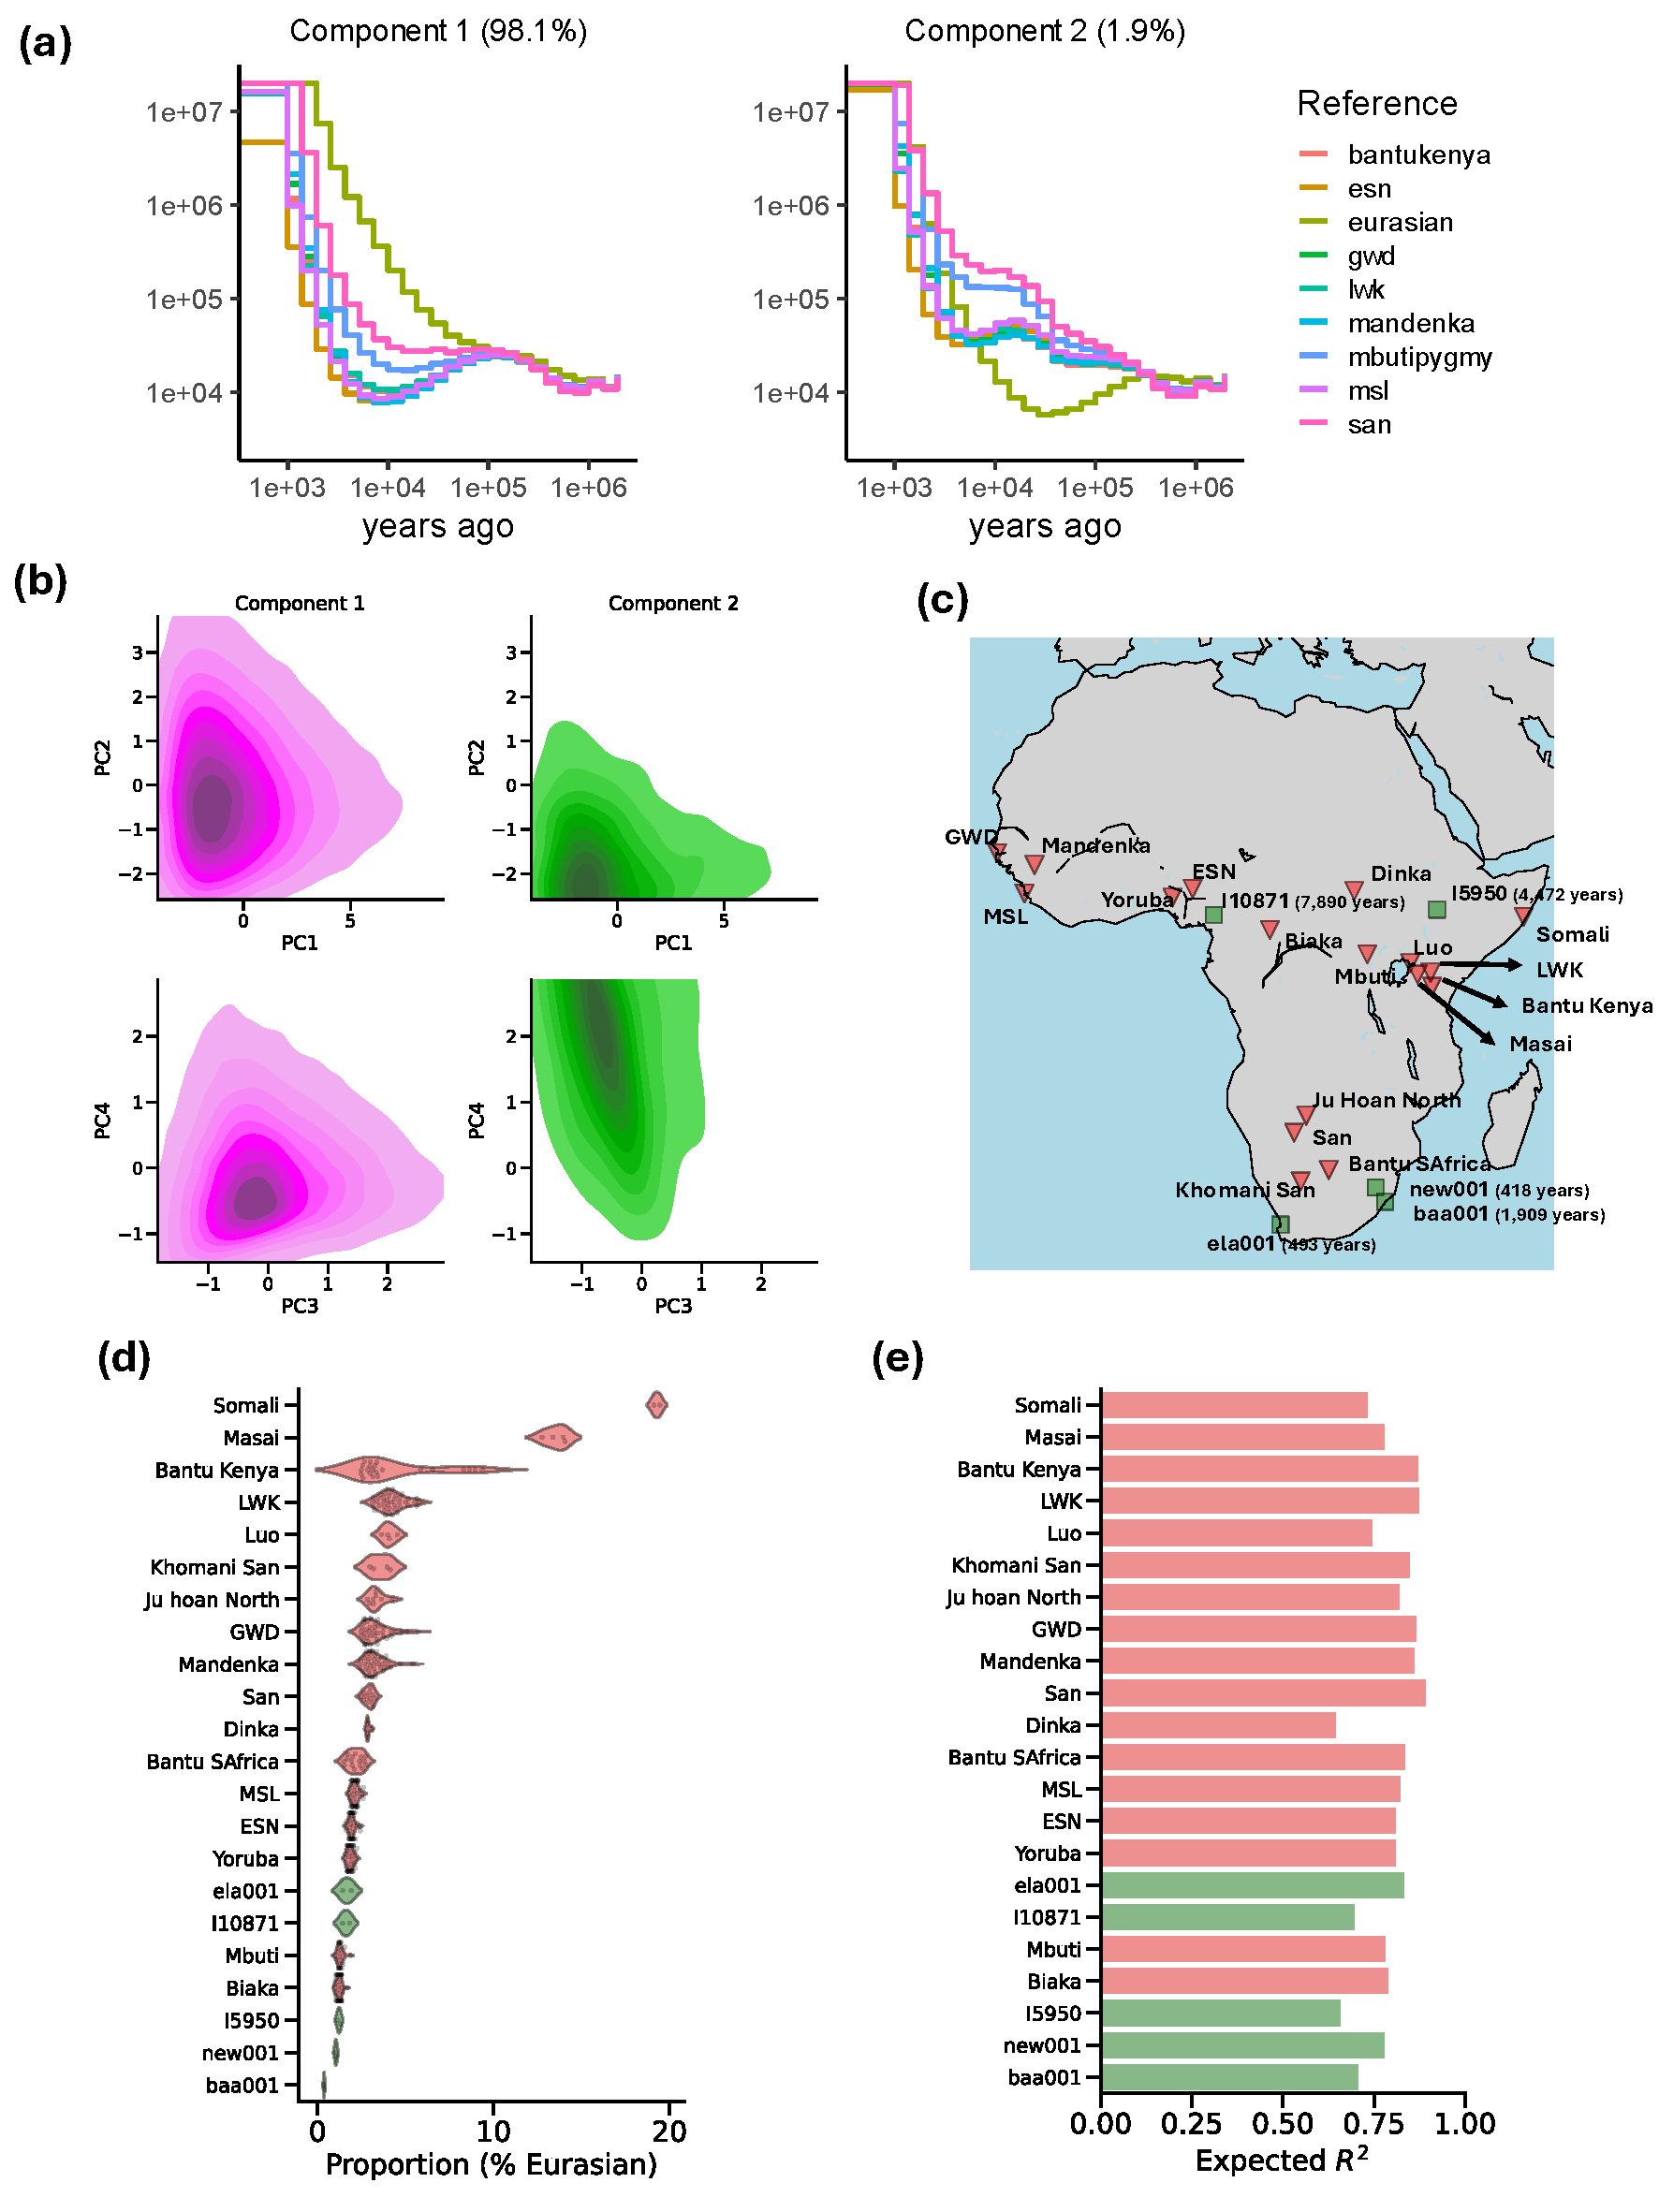
\includegraphics[width=\linewidth]{figures/gb_bta/gb_real_bta_1.pdf}
    \captionsetup{width=\textwidth+3cm}
    \caption{
    \footnotesize
    \textbf{Finding Eurasian-like ancestry in sub-Saharan Africans.} (a) Inferred inverse coalescence rates and proportions when decomposing Yorubans: each line represents inverse coalescence rate profiles with a reference population. (b) PCA visualization of the coalescence count and opportunity matrix derived from the genealogies plotted separately for each component. (c) Map of the African samples analyzed with red inverted triangles corresponding to modern samples in HGDP, $1{,}000$GP and SGDP, and green squares for 5 ancient African samples (with their estimated sampling ages in brackets). (d) Proportion of Eurasian-like ancestry and (e) Expected coefficient of determination across all African populations analyzed. The PCA visualization in (b) is based on a KDE plot with a threshold of 0.05, and binary local ancestry estimates are obtained by thresholding the inferred posteriors at 0.5. Individual data-points overlaid on the violin plots. 
    }
    \label{fig:gb_bta_1}
\end{figure}

\clearpage

\subsection{Dating the admixture event}
\label{sec:ch3-gb-bta-dating}

We dated these admixture events using coancestry curves derived from the local ancestry inferred by GhostBuster. To capture population-specific variation, we estimated admixture dates separately for each African population. However, for single-sample individuals, we could not apply the pseudo-individual normalization method described in Section \ref{sec:ch2-gb-coancestry}, which is critical for addressing population-specific drift and ensuring unbiased admixture date inference. We therefore do not report admixture dates for ancient individuals and the Somali population.

We fit the coancestry curves using three models: a single-date admixture model, a two-date admixture model, and a continuous admixture model with a constant migration rate. Our analysis revealed that a single admixture date did not adequately fit the coancestry curves for several African populations, as indicated by the visual fit of the coancestry curves and significant in-sample log-likelihood difference between the single-date and two-date admixture models ($> 20 \times \text{difference in number of parameters}$). This finding suggests a more complex genetic history (see Figure \ref{fig:gb_bta_3}a-c). Both the two-date and continuous admixture models provided an improved fit to the coancestry curves, as measured by the log-likelihood of the least squares fit. Notably, the two-date admixture model outperformed the continuous migration model in 14 out of 16 African populations (see Figure \ref{fig:gb_bta_3}d).

\begin{figure}[h!]
    \centering
    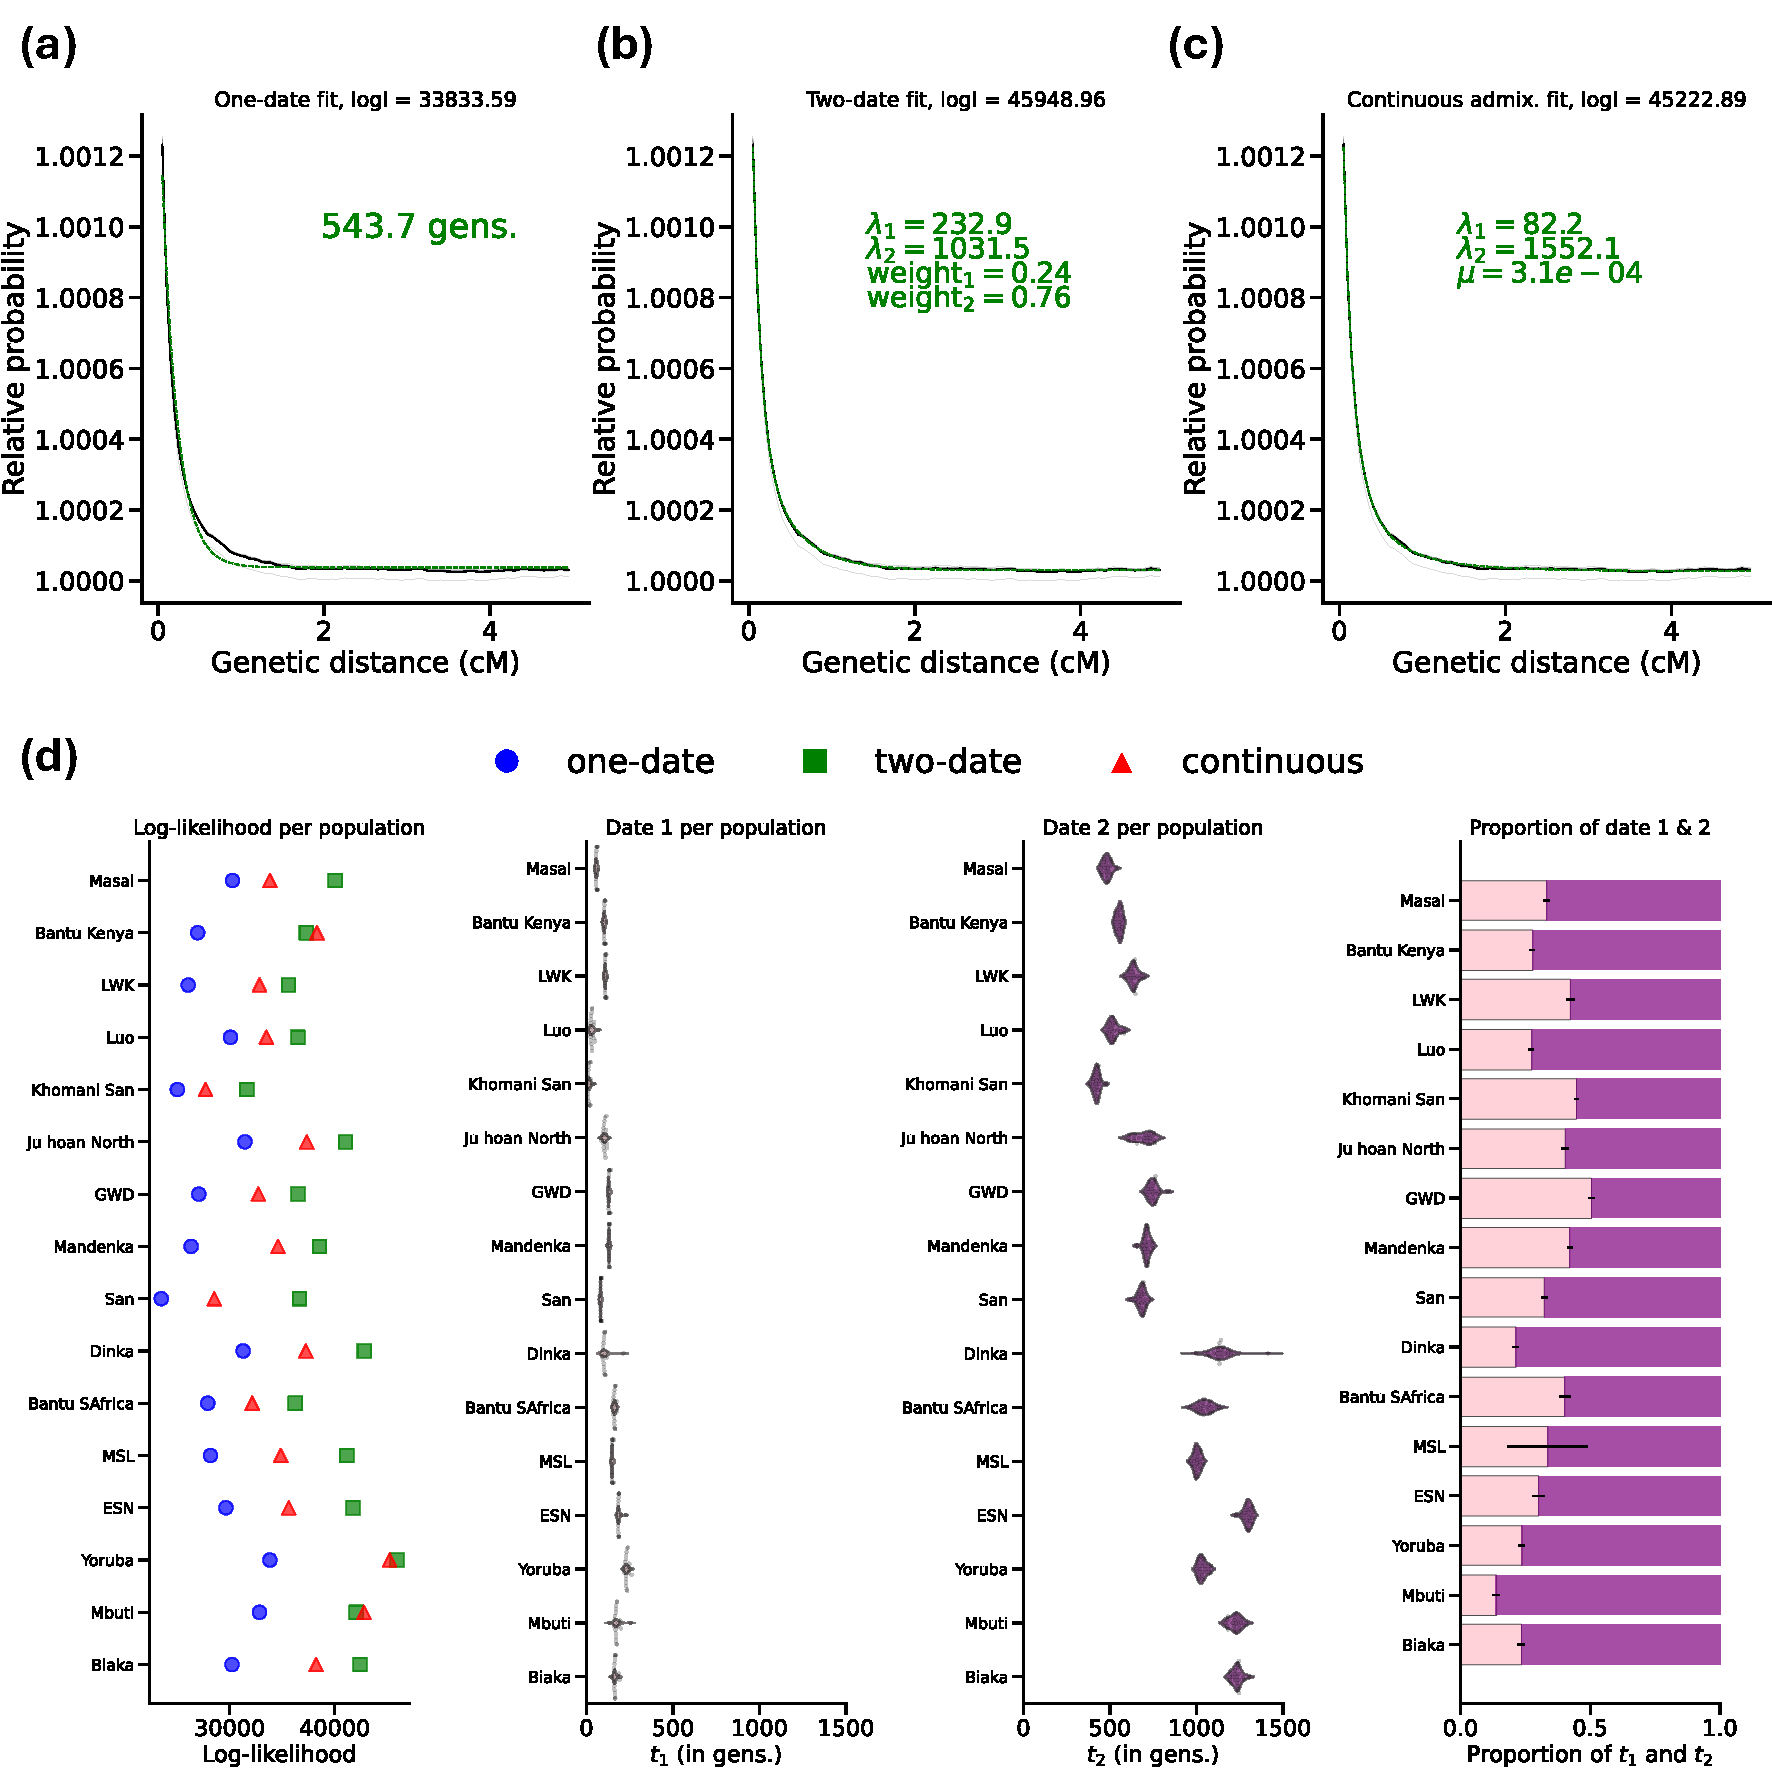
\includegraphics[width=\linewidth]{figures/gb_bta/gb_real_bta_3.pdf}
    \captionsetup{width=\textwidth+3cm}
    \caption{
    \footnotesize
    \textbf{Dating the Eurasian-like ancestry in sub-Saharan Africans.} Coancestry curves and (a) one-date admixture model fit, (b) two-date admixture model fit and (c) constant migration rate continuous admixture model fit for Yorubans. (d) Per-population least squared log-likelihood corresponding to various admixture models along with the admixture dates and weights inferred using two-date admixture model. The log-likelihood values are aggregated across $20$ jackknife runs. Populations are sorted based on highest to lowest proportion of Eurasian-like ancestry, pink represents the younger admixture date and purple represents the older admixture date in (d). Individual data-points overlaid on the violin plots. Admixture dates in the plot are in generations.
    }
    \label{fig:gb_bta_3}
\end{figure}

The two admixture dates exhibited considerable variation across geographic regions. In East African populations such as the Luhya (LWK), Bantu Kenya, Masai, and Luo, the more recent admixture event occurred $\leq 3{,}000$ years ago. In contrast, for West and Central African populations, including the Mende (MSL), Gambian (GWD), Mandenka, Esan (ESN), Yoruba, Mbuti, and Biaka, the recent admixture event is estimated to have occurred between $3{,}000$ and $7{,}000$ years ago. South African populations exhibited intermediate admixture dates ranging from $400$ to $4{,}500$ years ago, with the Khomani San showing the most recent admixture event at approximately $400$ years ago. The older admixture event dates were at least $15{,}000$ years old, ranging from $15{,}000$ to $35{,}000$ years across different African populations. Population-specific admixture dates and contributions are summarized in Figure \ref{fig:gb_bta_3}d and Table \ref{tab:gb_bta_admix_dates}. It is important to note that these admixture dates have not been adjusted for potential inaccuracies in the recombination map, as reliable error estimates were unavailable. This limitation may introduce a downward bias in the dating of the older admixture event \cite{sankararaman2012date}.

Given the distinct dates of these two admixture events, we perform separate validation analyses for each. To differentiate between the events, we first calculate the segment length of Eurasian ancestry segments by applying a threshold to the local ancestry posterior at \(50\)\%, then combining adjacent matching ancestry segments. Next, we estimate the posterior probability that a segment belongs to either the younger (typically in the last $10{,}000$ years) or older (typically between $15{,}000$ to $35{,}000$ years) admixture event for each population, using segment length as the determining factor. In particular, we use the admixture dates and proportions as inferred using per-population coancestry curve dating to assign this posterior. Given the assumption that segment lengths follow an exponential distribution conditioned on the admixture time, we proceed with the following model, given segment length $L$, admixture times $t_{\text{younger}}$ and $t_{\text{older}}$ and priors $p_{\text{younger}}$ and $p_{\text{older}}$ from coancestry curve dating:

\begin{align}
    \text{\textbf{Likelihood:} \vspace{2mm}} & \mathbb{P}(L | t) = t e^{-t * L} \nonumber \\
    \text{\textbf{Prior:} \vspace{2mm}} & \mathbb{P}(t = t_{\text{younger}}) = p_{\text{younger}}  = 1 - p_{\text{older}} \nonumber \\
    \text{\textbf{Posterior:} \vspace{2mm}} & \mathbb{P}(t = t_{\text{younger}} | L) = \frac{\mathbb{P}(L | t_{\text{younger}}) \cdot p_{\text{younger}}}{\mathbb{P}(L | t_{\text{younger}}) \cdot p_{\text{younger}} + \mathbb{P}(L | t_{\text{older}}) \cdot p_{\text{older}}} \nonumber \\
    & \mathbb{P}(t = t_{\text{older}} | L) = \frac{\mathbb{P}(L | t_{\text{older}}) \cdot p_{\text{older}}}{\mathbb{P}(L | t_{\text{younger}}) \cdot p_{\text{younger}} + \mathbb{P}(L | t_{\text{older}}) \cdot p_{\text{older}}}
\end{align}

We estimate the posterior probability of each position in the local ancestry belonging to either the younger or older admixture event. By combining these posterior estimates with GhostBuster's initial local ancestry inference, we obtain the probabilities that each segment represents either a younger or older Eurasian ancestry. Additionally, we construct histograms reflecting the segment length distribution for each population analyzed (see Figure \ref{fig:gb_segment_histogram}). In subsequent sections, we demonstrate that these younger and older Eurasian segments differ in their mutational signatures and levels of Neanderthal enrichment. We hypothesize that the younger Eurasian segments correspond to a back-to-Africa migration originating from Eurasia, while the older segments likely represent an ancient admixture event between African groups -- those who likely remained in Africa and those who migrated out of Africa. For much of the analysis in subsequent subsections, we focus primarily on the younger segments to highlight their distinct properties relative to the older segments. However, a detailed analysis of the older admixture segments is conducted in further Section \ref{sec:ch3-gb-deep}.

% \clearpage

\subsection{Eurasian ancestry explains the Neanderthal ancestry in Africans}

Previous research has shown that modern Africans carry small amounts of Neanderthal ancestry in their genomes, likely due to a back-migration event from Europe \cite{chen2020identifying, bergstrom2020insights, wang2013apparent, hollfelder2017northeast}. We look for this Neanderthal ancestry as a way to validate the Eurasian segments identified in our analysis. Specifically, we used GhostBuster to detect Neanderthal ancestry in African individuals by jointly analyzing genealogies inferred from both modern African samples and ancient samples, including three Neanderthal genomes from the Altai, Chagyrskaya, and Vindija caves.

Our analysis focused on coalescence events that occurred between $50{,}000$ and 2 million years ago, partitioning this time frame into 20 epochs on a logarithmic scale. To specifically detect Neanderthal segments rather than other ancient events, we restricted the analysis to coalescence events with sequenced Neanderthals only, ignoring the rest of the tree. We began by setting the cluster coalescence rates to genome-wide coalescence rates observed between sequenced Neanderthals themselves and the target African populations. Using these predefined coalescence rates, we employed the EM algorithm to estimate admixture proportions, admixture time, and local ancestry across the sample. In the final iteration of the EM algorithm, we update the coalescence rates based on the inferred local ancestry instead of using the pre-specified genome-wide coalescence rates. This adjustment fine-tunes the estimates to account for differences between the Neanderthal sources that contributed ancestry to Africans and the sequenced Neanderthals, allowing us to obtain unbiased and accurate estimate of Neanderthal local ancestry in African genomes. 

To validate our approach for detecting Neanderthal ancestry, we first estimated Neanderthal ancestry in Eurasians, recovering approximately $1$–$2$\% across six modern Eurasian groups (see Figure \ref{fig:gb-bta-nea-eurasians}). These proportions align with prior findings \cite{prufer2014complete,skov2020nature}. East Asian populations exhibited approximately $20$\% higher Neanderthal ancestry, with an average of $1.5$\%, compared to South Asians and Europeans, which showed about $1.25$\% Neanderthal ancestry -- consistent with previous studies \cite{meyer2012high,iasi2024neandertal}. Furthermore, we observed little to no Neanderthal ancestry in genomic regions previously identified as ``archaic deserts'' \cite{sankararaman2016combined,vernot2016excavating} (see Figure \ref{fig:gb-bta-nea-eurasians}d).  It is important to note our approach circumvents the need for un-admixed reference samples or identity-by-descent (IBD) segments with Neanderthals, and utilizes the entire coalescence history with sequenced Neanderthal directly, making it more robust and powerful for finding Neanderthal ancestry in Africans.  

We found that African samples from the HGDP+$1{,}000$GP dataset exhibit approximately \( 0.004\% \) to \( 0.056\% \) Neanderthal ancestry, with the lowest levels observed in Mbuti individuals and the highest levels in Bantu Kenyans, among the populations analyzed. Figure \ref{fig:gb_bta_nea}a shows the inverse coalescence rates for Neanderthal ancestry in Yoruba (as a representative population). Our analysis revealed a strong correlation between the genome-wide Neanderthal proportion and the Eurasian-like ancestry proportion inferred with GhostBuster, yielding a correlation \( R^2 = 0.51 \). To examine Neanderthal ancestry correlations associated with the younger and older admixture events, we fitted a joint regression model to predict Neanderthal ancestry proportion based on the proportions of younger and older Eurasian ancestry within individuals. The younger Eurasian ancestry proportion had a slope of \(1.22\%\), whereas the older Eurasian ancestry showed a slope of \(0.67\%\). These slopes represent the increase in Neanderthal ancestry per unit increase in Eurasian-like ancestry, effectively quantifying the proportion of Neanderthal ancestry within these Eurasian segments. The joint regression also inferred an intercept not significantly different from $0$ at $0.009$\%. This suggests a probable absence of Neanderthal ancestry in non-Eurasian-like segments and highlights a disparity in Neanderthal ancestry between the two Eurasian-like segments identified in Africa (see Figure \ref{fig:gb-bta-nea-supp2}). 
%It is also possible the older admixture ancestry lacks Neanderthal ancestry completely due to presence of short segments corresponding to younger admixture event misclassified as older admixture event.

At the local ancestry level, we defined the enrichment of Neanderthal ancestry within Eurasian segments as the mean local ancestry posterior for Neanderthal ancestry in Eurasian segments (determined by a local ancestry threshold of 0.5) divided by the mean posterior in non-Eurasian segments. Under a model with no correlation between Neanderthal and Eurasian-like ancestry in Africa, this enrichment should be close to unity. However, we observed a \(21.9\times\) enrichment of Neanderthal ancestry within Eurasian segments compared to non-Eurasian segments (see Figure \ref{fig:gb_bta_nea}b). Further stratification of Eurasian segments by length showed even higher enrichment for longer segments and lesser enrichment for shorter segments: \( 31.4\times \) for segments longer than \(0.5\)cM, \( 23.1\times \) for segments between \(0.2\) and \(0.5\)cM, \( 11.3\times \) for segments between \(0.1\) and \(0.2\)cM, and \( 4.3\times \) for segments shorter than \(0.1\)cM. 

The disparity in estimated coefficients for older and younger admixture in Figure \ref{fig:gb-bta-nea-supp2}, combined with reduced enrichment in shorter segments, suggests the possibility that Neanderthal ancestry is entirely absent from the older admixture event and the reduced signal is only driven by misassignment of segments originating from the more recent event to the older event. To obtain more robust estimates of Neanderthal local ancestry while minimizing false-positive rates, we recalculated Neanderthal ancestry in Africans by masking non-Eurasian-like segments and only using the Eurasian-like segments during coalescence rate inference. This masking produced genome-wide proportions of Neanderthal ancestry that were comparable to the original run without masking (paired t-test, $p=0.18$).

We dated the admixture event using Eurasian segments that specifically contained at least one Neanderthal segment. This analysis aimed to determine whether Neanderthal ancestry was present in both the younger and older Eurasian segments. If a date exceeding $20{,}000$ years is detected, it would indicate that the older Eurasian segments also carried Neanderthal ancestry. Conversely, detecting only more recent admixture dates would suggest that Neanderthal ancestry arrived exclusively through the more recent admixture event. We constructed coancestry curves using hard-called local ancestry, where Eurasian-like segments with Neanderthal ancestry (posterior probability $\geq 0.1$) at at least one position were assigned a value of 1, while all other regions, including Eurasian-like segments without Neanderthal ancestry, were assigned a value of 0. We then fit multiple admixture models to the generated coancestry curves. Our analysis revealed that a single admixture date provides an adequate (in-sample log-likelihood difference between single- and two-date admixture models $< 2 \times \text{difference in number of parameters}$, see Figure \ref{fig:gb-bta-nea-supp3}) fit for most African populations, with some exceptions. For instance, populations such as Bantu Kenya from East Africa fit better with a two-admixture-date model. Similarly, West African populations like Gambian (GWD) and Mende (MSL) also showed a slight improvement with a two-admixture-date model, though these estimates were more noisy (see Figure \ref{fig:gb-bta-nea-supp3}). The admixture dates corresponding to both single- and two-date models for some populations ranged approximately from 4,000 to 10,000 years ago (see Figure \ref{fig:gb_bta_nea}c-d). These admixture dates fall within the range of the younger admixture dates inferred previously in Section \ref{fig:gb_bta_3}, and are not consistent with the older admixture date. This suggests that the older admixture date, which occurred approximately $15{,}000$ - $35{,}000$ years ago, did not carry Neanderthal ancestry. Furthermore, admixture dates varied based on the present-day geographic location of samples. West African populations, such as Yoruba and Esan, exhibited the oldest admixture dates, approaching $10{,}000$ years ago -- aligning with the green Sahara period \cite{tierney2017rainfall, larrasoana2013dynamics} and well before the expansion of Bantu-speaking peoples. Central African hunter-gatherers, including Mbuti individuals, exhibit minimal Neanderthal ancestry, leading to noisier coancestry curve dating and were therefore excluded from the main figure. More detailed results, including the dating of Neanderthal ancestry in Mbuti individuals, can be found in Figure \ref{fig:gb-bta-nea-supp3}. These findings suggest that the Neanderthal ancestry present in Africans is predominantly associated with the younger admixture event, which occurred during the Holocene, starting shortly after the end of the last Ice Age.

To further validate our hypothesis that the older Eurasian segments do not carry substantial Neanderthal ancestry, we analyzed the mean posterior probability of Neanderthal ancestry as a function of segment length. We compared the empirical estimates of mean Neanderthal posterior probabilities to theoretical predictions from a two-date admixture model, under the assumption that only the younger admixture event contributes Neanderthal ancestry. The theoretical model is defined as follows:
\begin{align}
    P ( L \leq l | \text{model}_{\text{younger}}) &= 1 - e^{-lt_{\text{younger}}} \nonumber \\
    P ( L \leq l | \text{model}_{\text{older}}) &= 1 - e^{-lt_{\text{older}}} \nonumber \\
    P ( \text{Neanderthal} | \text{model}_{\text{younger}}) &= \alpha \nonumber \\
    P ( \text{Neanderthal} | \text{model}_{\text{older}}) &= 0 \nonumber \\
    P ( \text{model}_{\text{younger}}) = 1 - P ( \text{model}_{\text{older}}) &= p_{\text{younger}}
\label{eq:gb_nea_segm_1}
\end{align}
where, $\text{model}_{\text{younger}}$ and $\text{model}_{\text{older}}$ correspond to Eurasian-like ancestry in Africans derived from the younger and older admixture events, respectively. Here, $\alpha$ represents the proportion of Neanderthal ancestry in the Eurasian source population contributing to the younger admixture event; $t_{\text{younger}}$ and $t_{\text{older}}$ are the admixture dates, and $p_{\text{younger}}$ is the proportion of ancestry contributed by the younger admixture event. These parameters are estimated using the coancestry curves presented in Section \ref{sec:ch3-gb-bta-dating}. Based on the Equation \ref{eq:gb_nea_segm_1}, the probability of Neanderthal ancestry conditioned on segment length can be expressed as:
\begin{align}
    P( \text{Neanderthal} | L \leq l) = \frac{\alpha p_{\text{younger}} (1 - e^{-lt_{\text{younger}}})}{p_{\text{younger}} (1 - e^{-lt_{\text{younger}}}) + (1 - p_{\text{younger}}) (1 - e^{-lt_{\text{older}}})}
\end{align}

We estimated confidence intervals for the theoretical models by incorporating uncertainties in coancestry dating. Our results showed that the theoretical model, assuming no Neanderthal ancestry from the older admixture event, fit the empirical data well across several populations (see Figure \ref{fig:gb-bta-nea-supp}). This finding further supports the hypothesis that the older admixture event did not contain substantial Neanderthal ancestry. 
% However, some populations, including the San, Mbuti, and Yoruba, deviated from the theoretical curves. These discrepancies suggest the possibility of multiple sources of Neanderthal ancestry, including contributions from the older admixture event for some of these populations.

Finally, we analyzed Neanderthal content in ancient African samples, finding \( 0.026\% \) and \( 0.017\% \) Neanderthal ancestry in ela001 ($493$ years) and new001 ($418$ years) individuals respectively, and \( 0.01\% \) in the $1{,}900$-year-old Ballito Bay individual (baa001). In contrast, we detected no Neanderthal ancestry (\(<10^{-9}\%\)) in ancient samples from the Mota Cave ($4{,}472$ years) and Cameroon ($7{,}890$ years). This again suggests that the younger admixture event which might be missing in Mota and Cameroon individuals contributed Eurasian-like ancestry with detectable Neanderthal ancestry, whereas the older admixture event might be associated with reduced or no Neanderthal ancestry.

\begin{figure}[h!]
    \centering
    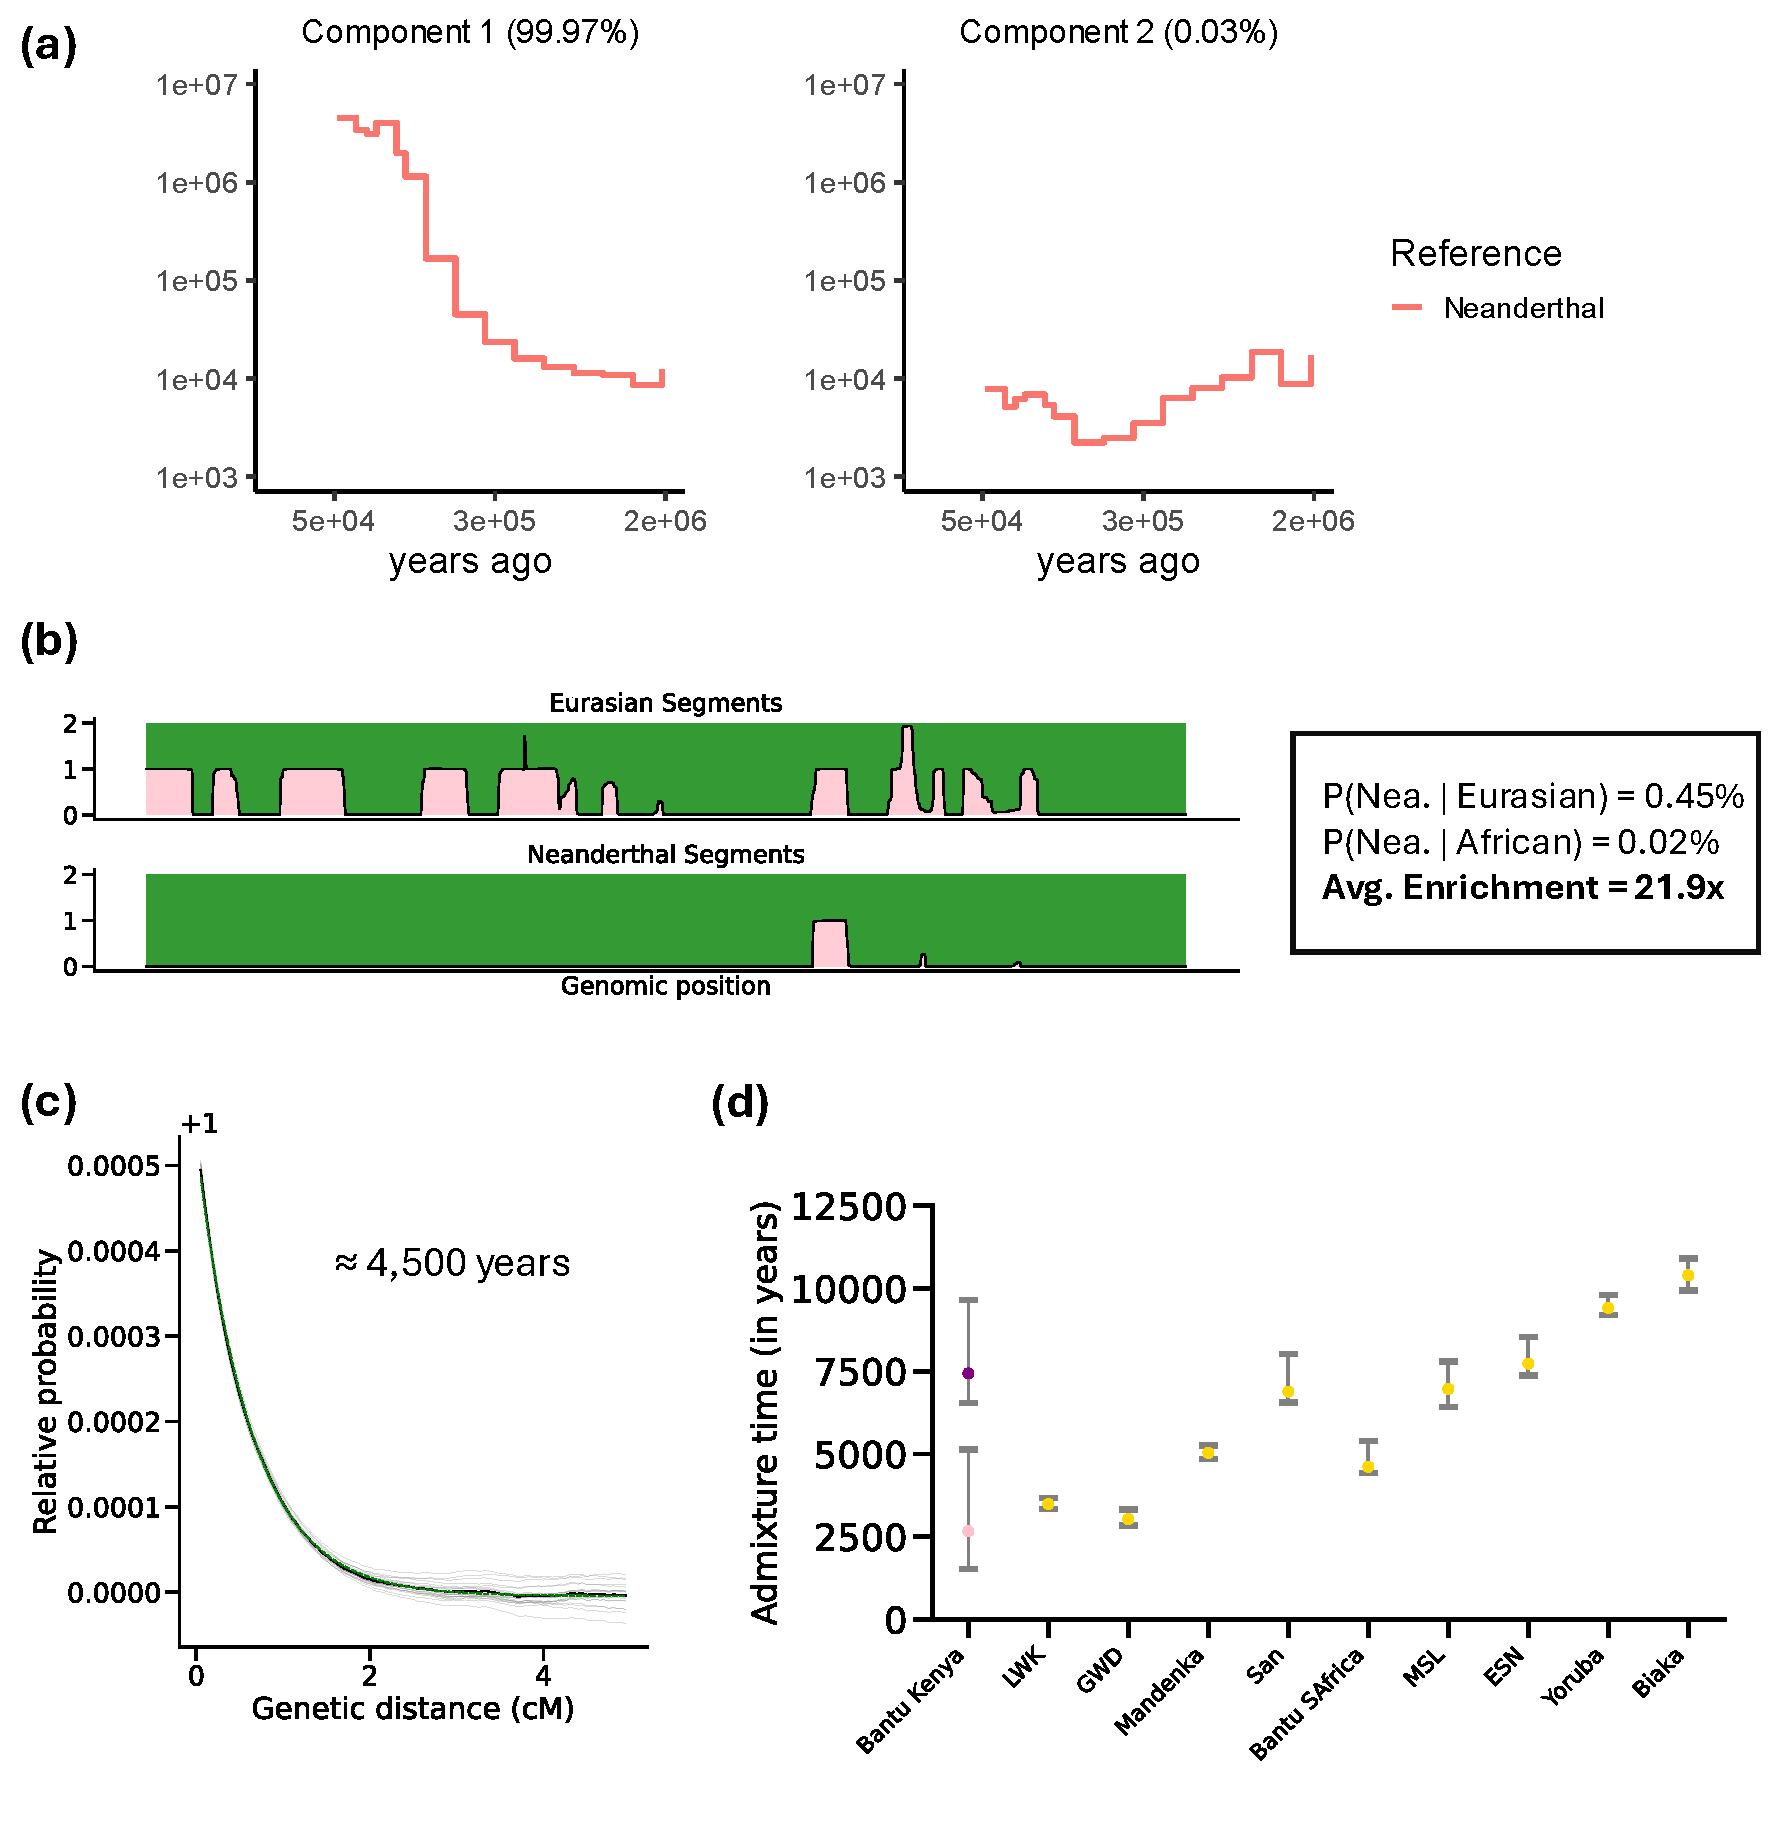
\includegraphics[width=\linewidth]{figures/gb_bta/gb_real_bta_6.pdf}
    \captionsetup{width=\textwidth+3cm}
    \caption{
    \footnotesize
    \textbf{Eurasian ancestry explains the Neanderthal ancestry in Africans.} (a) Inferred inverse coalescence rates and proportions for Neanderthal ancestry in Yorubans: the line represents the inverse coalescence rate profiles with sequenced Neanderthals. (b) Sample HGDP01405 showing a 20 Mb region enriched for Neanderthal ancestry, overlapping Eurasian-like segments. The average enrichment is calculated as the ratio of the mean posterior probability of Neanderthal ancestry in Eurasian segments, $P(\text{Nea} \mid \text{Eurasian})$, to the mean posterior probability in African segments, $P(\text{Nea} \mid \text{African})$. (c) Coancestry curve showing the normalized joint probability and single admixture date fit for Eurasian segments carrying Neanderthal ancestry, averaged across all African samples analyzed. (d) Admixture dates derived from coancestry curves generated by Eurasian segments carrying Neanderthal ancestry for each population. For Bantu Kenya a two-date admixture model fit is shown, as it better explains the coancestry patterns. More detailed results are provided in Figure \ref{fig:gb-bta-nea-supp3}. Grey lines in (c) and error bars in (d) represent jackknife estimates and 95\% confidence intervals around the mean. For panel (d) single date admixtures shown in golden, whereas two date admixtures shown in pink and purple. Results derived from HGDP+$1{,}000$GP+aDNA+archaic genealogies.}
    \label{fig:gb_bta_nea}
\end{figure}


\clearpage

\subsection{Mutational profiles validate Eurasian segments in Africans}
\label{sec:ch3-gb-bta-mutational}

Evidence suggests that human mutation rates have evolved over short time scales and independently across different populations \cite{harris2015evidence, harris2017rapid}. One notable example is the TCC to TTC mutation, which occurs at up to twice the rate in West Eurasian groups compared to East Asians or Africans. Another example is GC-biased gene conversion (GCbGC) \cite{duret2009biased}, which preferentially selects GC alleles (termed ``strong'') over AT alleles (termed ``weak''). GCbGC is influenced by factors such as population size and recombination hotspots: populations with larger effective population sizes or fewer bottlenecks exhibit higher rates of weak to strong mutations than populations with reduced population sizes. Figure \ref{fig:gb_bta_ws_vs_sw} illustrates the evolution of weak to strong mutations relative to strong to weak mutations across various continental populations.

To investigate this within the context of the back-migration event, we define the normalized mutation rate similar to the Relate \cite{speidel2019method} paper for a specific mutation type (example, TCC to TTC, or weak to strong) in a given population. This normalized mutation rate (NMR) is calculated as the ratio of the number of mutations of that specific type that have arisen in the population to the number of mutations of all other types that have arisen in the same population. Formally, this is expressed as:
\begin{equation}
    \text{NMR}_{\text{pop, type}} = \frac{\sum_{mut} \mathbbm{1}(mut \in \text{type}) \, N_{mut, pop}}{\sum_{mut} \mathbbm{1}(mut \notin \text{type}) \, N_{mut, pop}}
\end{equation}
where, $\sum_{mut}$ sums all the mutations in the genealogy, $N_{mut, pop}$ counts the number of individuals belonging to population `pop' carry the mutation `mut'. We further stratify mutation rates by allele age, dividing them into 10 epochs ranging from $1{,}000$ years to 1 million years. To facilitate meaningful comparisons, we further divide these normalized mutation rates (NMR) and the normalized mutation rates (NMR) in African populations:
\begin{equation}
    \text{NMRE}_{\text{pop, type}} = \frac{\text{NMR}_{\text{pop, type}}}{\text{NMR}_{\text{AFR, type}}}
\end{equation}
This measure, referred to as the Normalized Mutation Rate Enrichment (NMRE), quantifies the relative enrichment of specific mutation types in a given population compared to their normalized mutation rates in Africans. A significant deviation from unity indicates that the specific mutation type is either enriched (greater than 1) or depleted (less than 1) in the population relative to the African baseline. We examine this enrichment across various continental populations, including all non-Finnish Europeans (NFE), East Asians (EAS), South Asian (SAS) and Middle Eastern and North African (MID) groups in HGDP. Notably, we analyze the enrichment for Eurasian and non-Eurasian segments in African samples separately. To correct for mutational biases in local ancestry fitting, we down-sample Eurasian and non-Eurasian segments at each location to equalize the number of descendants in both categories. We perform $1{,}000$ chromosome-wise bootstraps to estimate the confidence interval around the normalized mutation rate enrichment. 

Examining the TCC to TTC mutation types, we observe significant enrichment not only in European, Middle Eastern, and South Asian populations but also in the Eurasian-like segments within African individuals. In Figure \ref{fig:gb-mut-tcc}a,b, this enrichment is plotted separately for Eurasian segments, conditioned on their segment lengths. Both long and short Eurasian segments in Africans exhibit significant enrichment in TCC to TTC mutations during the period from $1{,}000$ to $40{,}000$ years ago, consistent with the evolutionary trajectory of these mutations, which rose sharply around $15{,}000$ years ago and declined approximately $2{,}000$ years ago \cite{harris2017rapid}. The enrichment is particularly pronounced in longer Eurasian segments, which are more likely to be associated with the younger admixture date, peaking at approximately $2\times$ around $20{,}000$ years ago -- levels comparable to those observed in Europeans. This pattern suggests a European source as the most probable origin for the back-to-Africa migration.

%We did not detect this enrichment in Africans before due to the limited proportion of Eurasian segments in their genomes. However, by leveraging local ancestry inferred through GhostBuster, we were able to isolate and identify this enrichment, providing independent validation of the back-migration event we identified.  

\begin{figure}
    \centering
    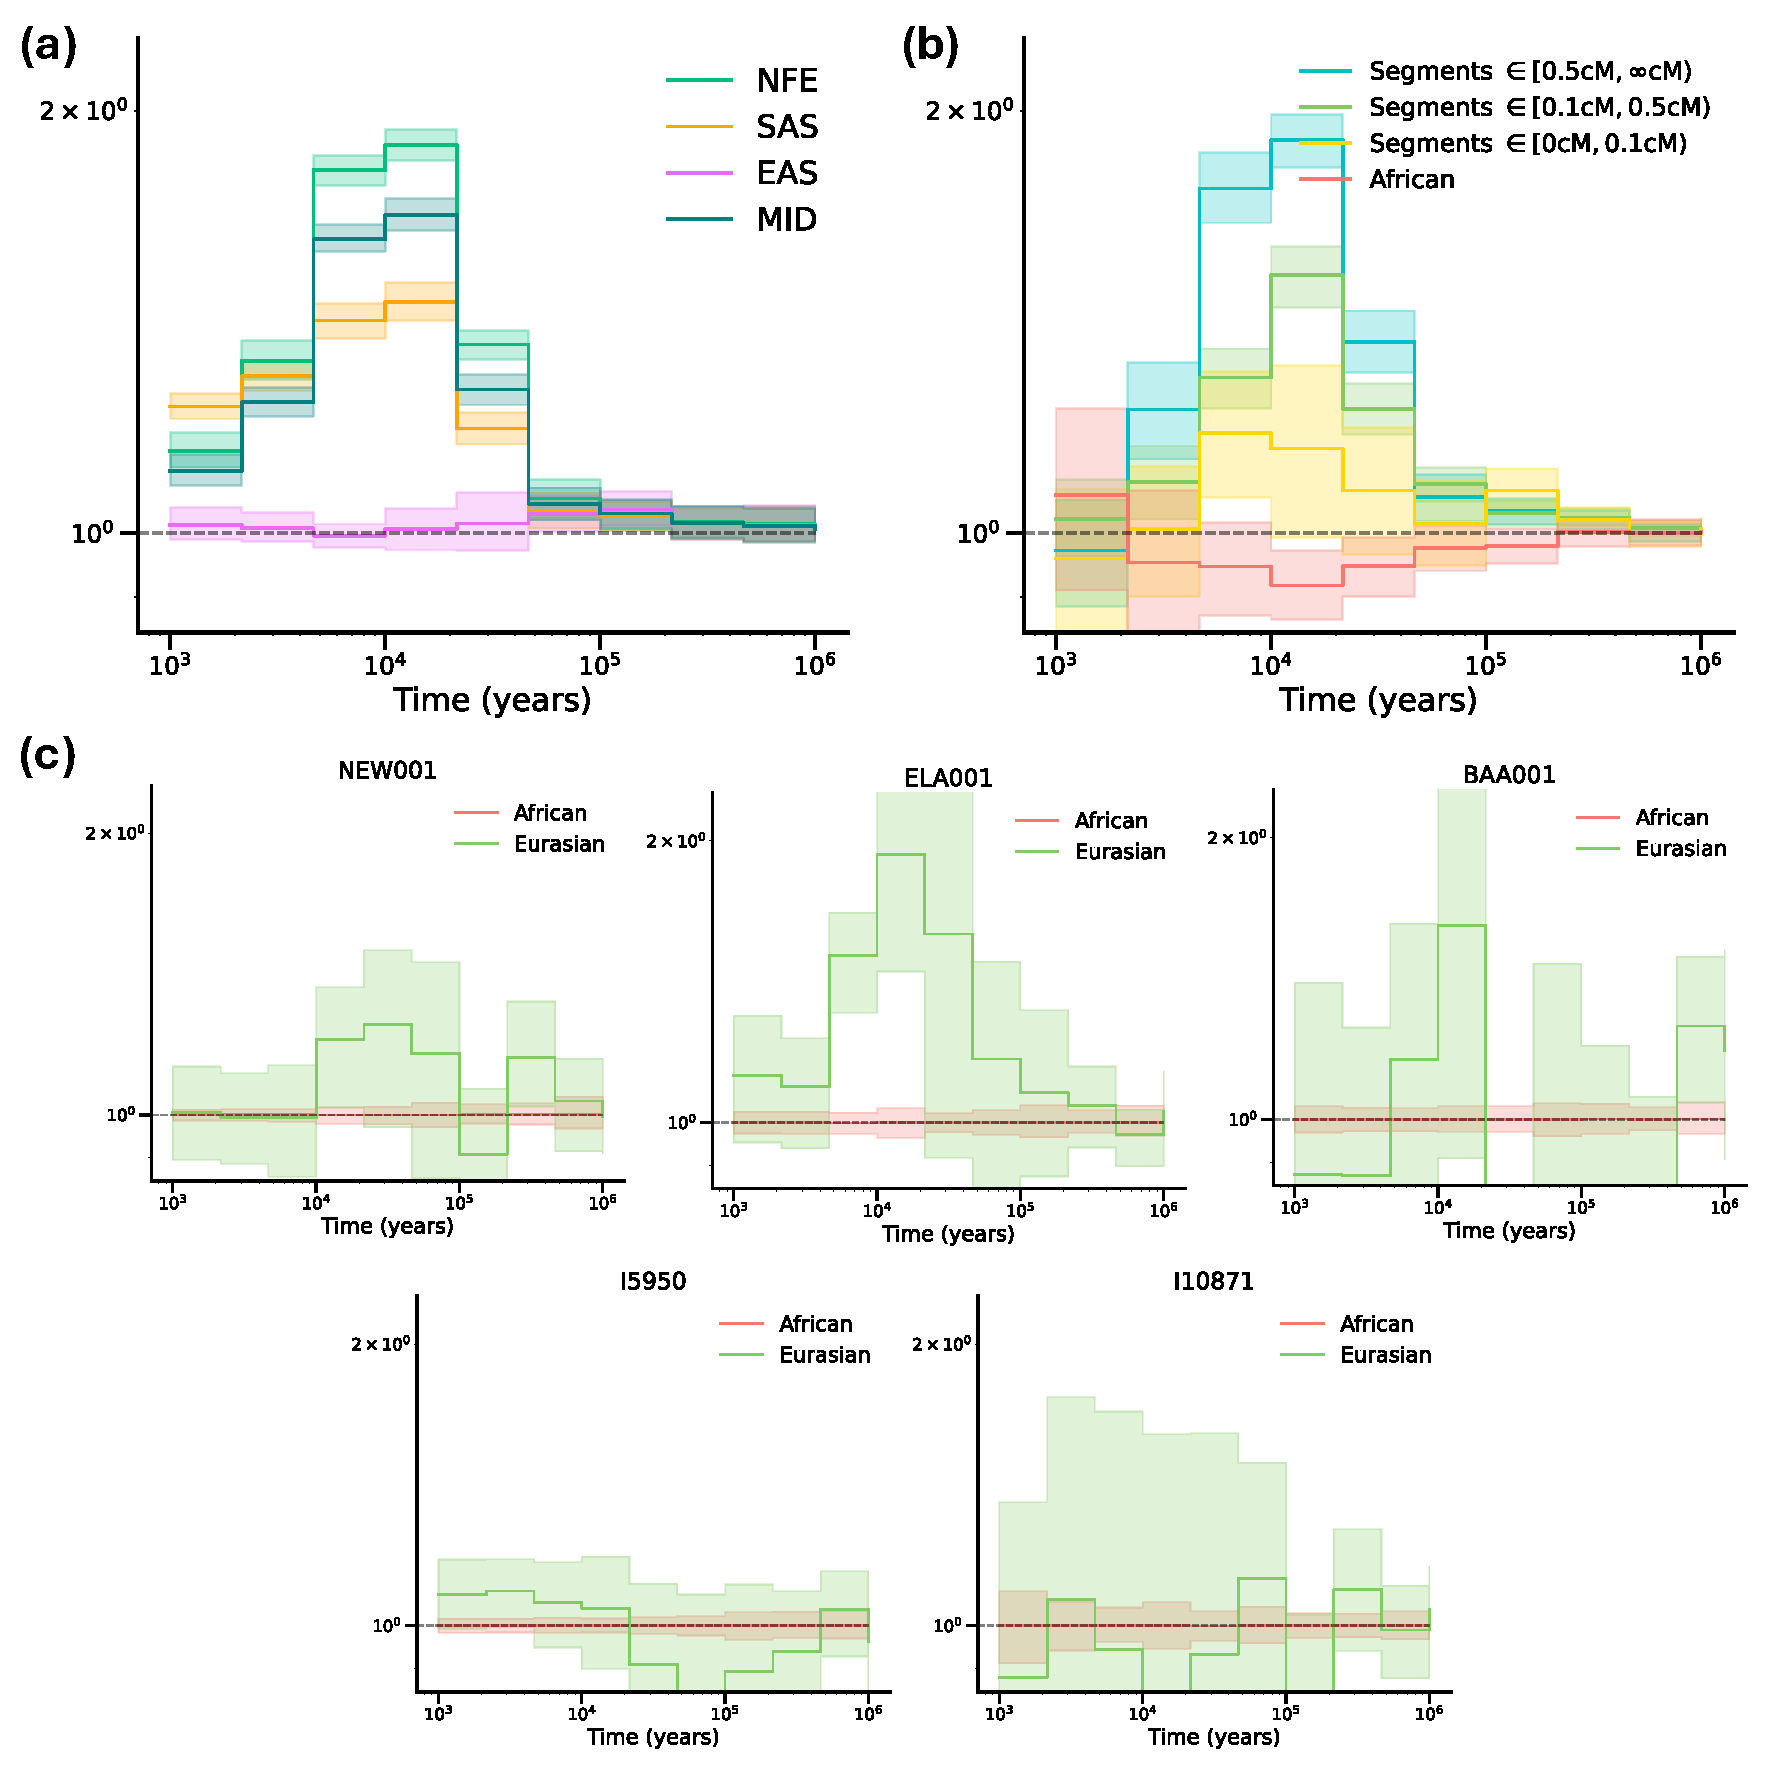
\includegraphics[width=\linewidth]{figures/gb_bta/gb_real_bta_8.pdf}
    \captionsetup{width=\textwidth+3cm}
    \caption{
    \footnotesize
    \textbf{Enrichment of TCC to TTC mutation rates in African components.} (a) Enrichment of TCC to TTC mutation rates across various continental groups, including NFE (non-Finnish Europeans), SAS (South Asians), EAS (East Asians), and MID (Middle Eastern and North African populations). (b) Enrichment of TCC to TTC mutation rates in Eurasian and non-Eurasian (African) segments in African populations. (c) TCC to TTC mutation rate enrichment in five ancient African samples, including new001, ela001, baa001, I5950, and I10871 (see population descriptions in Table \ref{tab:african_populations_2}). Shaded regions indicate 95\% confidence intervals derived from $1{,}000$ bootstrap replicates, while the dashed line represents the baseline of no enrichment. In panel (b), the Eurasian segments in Africans are further categorized based on their lengths: segments shorter than 0.1 cM, those between 0.1 and 0.5 cM, and segments longer than 0.5 cM. Results derived from HGDP+$1{,}000$GP and HGDP+$1{,}000$GP+aDNA+archaic genealogies.
    }
    \label{fig:gb-mut-tcc}
\end{figure}

We conducted this analysis across various African populations and consistently found enrichment in Eurasian segments across all groups. Populations with more recent admixture, such as the San, Bantu Kenya, and Mandenka, exhibited the highest enrichment, while those with older admixture events, such as the Mbuti, Biaka, and Yoruba, showed weaker enrichment for TCC to TTC mutations. Notably, some African populations, including the San and Bantu Kenyans, displayed empirical enrichment levels exceeding the average across all non-Finnish Europeans (see Figure \ref{fig:gb-mut-tcc-pops}). In our analysis of ancient African samples, similar enrichment patterns emerged, though with increased variability due to smaller sample sizes. We normalized mutation rates in ancient samples relative to the mutation rates in their African segments, rather than using mutation rates from modern African samples, to minimize the impact of differences in sampling times and biases associated with ancient DNA genealogy construction. We observed modest enrichment in more recent ancient samples from South Africa, whereas older samples from Mota Cave and Cameroon showed no detectable enrichment (see Figure \ref{fig:gb-mut-tcc}c). This absence of enrichment in older samples could be attributed to statistical noise when detecting TCC to TTC mutation enrichment in individual ancient samples or might indicate a lack of back-to-Africa admixture signals in these older populations.

In addition to examining the TCC to TTC mutations, we also investigated the enrichment of mutations related to weak to strong mutation types. For our analysis, we excluded CpG sites when defining weak or strong mutations. Similar to patterns observed in European, East Asian, and South Asian populations, the Eurasian segments within African genomes also showed reduction for weak to strong mutations relative to African genomes as a whole. The reduction in weak-to-strong mutations reached its peak approximately $50{,}000$–$100{,}000$ years ago, aligning with patterns observed in other Eurasian populations. Interestingly, Eurasian segments of all lengths in Africans exhibit a similar pattern of weak to strong mutation reduction, and with a slightly lower amplitude compared to that observed in Europeans and East Asians. This pattern suggests that the Eurasian-like ancestry in African genomes may have experienced an even more pronounced bottleneck than the population that initially migrated out of Africa (see Figure \ref{fig:gb-mut-ws}a,b). As with TCC to TTC enrichment, we stratified the weak to strong mutation reduction by population and ancient samples. We found consistent levels of weak to strong reduction across all modern populations and ancient samples, suggesting that both the younger and older admixture events may have undergone a population bottleneck approximately $50{,}000$–$100{,}000$ years ago (see Figure \ref{fig:gb-mut-ws}c and \ref{fig:gb-mut-ws-pops}). Finally, we present the mutation rate enrichment for Eurasian-like versus non-Eurasian-like segments in Africans across all 96 trimer mutation types, as shown in Figure \ref{fig:gb-mutational-all-bta}.

\begin{figure}
    \centering
    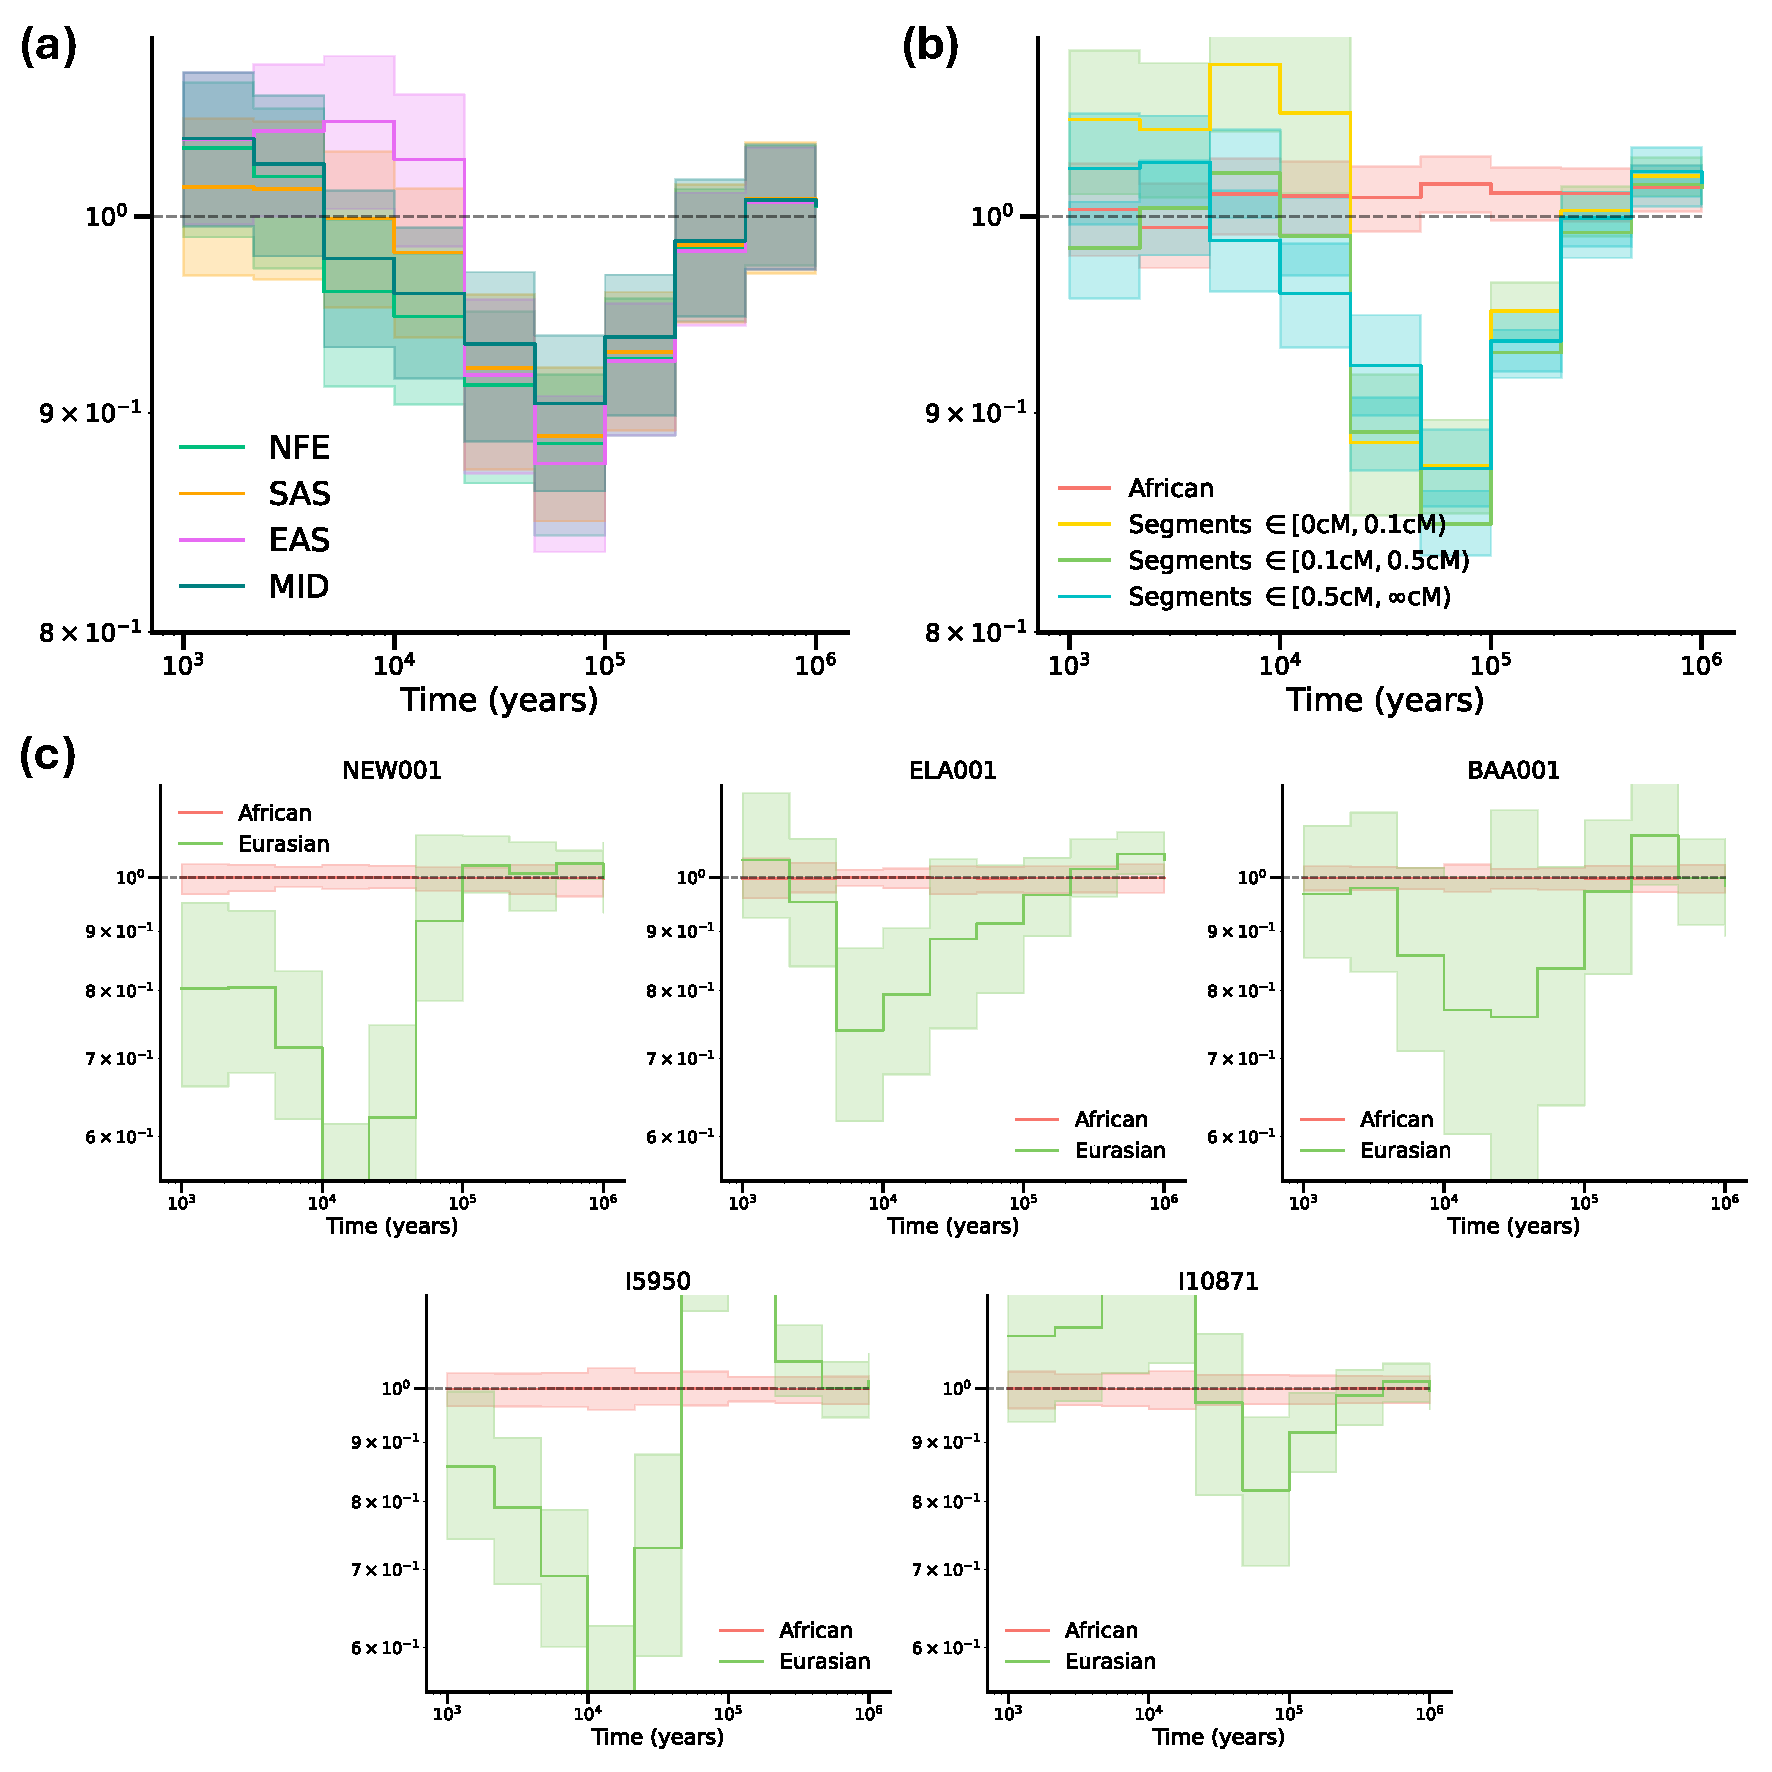
\includegraphics[width=\linewidth]{figures/gb_bta/gb_bta_real_10.pdf}
    \captionsetup{width=\textwidth+3cm}
    \caption{
    \footnotesize
    \textbf{Enrichment of weak to strong mutation rates in African components.} (a) Enrichment of weak to strong mutation rates across various continental groups, including NFE (non-Finnish Europeans), SAS (South Asians), EAS (East Asians), and MID (Middle Eastern and North African populations). (b) Enrichment of weak to strong mutation rates in Eurasian and non-Eurasian (African) segments in African populations. (c) weak to strong mutation rate enrichment in five ancient African samples, including new001, ela001, baa001, I5950, and I10871 (see population descriptions in Table \ref{tab:african_populations_2}). Shaded regions indicate 95\% confidence intervals derived from $1{,}000$ bootstrap replicates, while the dashed line represents the baseline of no enrichment. In panel (b), the Eurasian segments in Africans are further categorized based on their lengths: segments shorter than 0.1 cM, those between 0.1 and 0.5 cM, and segments longer than 0.5 cM. Results derived from HGDP+$1{,}000$GP and HGDP+$1{,}000$GP+aDNA+archaic genealogies.
    }
\label{fig:gb-mut-ws}
\end{figure}


\clearpage

\subsection{Identifying source populations for Eurasian ancestry}
\label{sec:ch3-gb-bta-source}

To characterize the admixture event and identify potential source populations contributing Eurasian-like ancestry to Africa, we calculated coalescence rates using modern samples from the HGDP+$1{,}000$GP dataset and a subset of 40 high-coverage ancient samples with estimated sampling ages less than $10{,}000$ years and sampled in Eurasia or Africa (see Table \ref{tab:gb_ancient_samples} for list of all ancient samples). For clarity, we grouped ancient samples corresponding to Neolithic Anatolian and Balkan farmers into one group, and Western Hunter-gatherers into one group. We used Colate \cite{speidel2021inferring} with the \texttt{--mode local\_ancestry} flag to infer the coalescence rates conditioned on the local ancestry in African samples. We analyzed Eurasian-like segments associated with both recent and ancient admixture events separately, with a primary focus on understanding the recent Eurasian-like segments. Furthermore, to capture population-specific variations in Eurasian ancestry, we conducted analyses for each African population separately. 

To understand coalescence relationships across populations, we focused on the epoch spanning $10{,}000$–$16{,}000$ years and constructed a pairwise coalescence rate matrix. This matrix was visualized using a heatmap, a clustering dendrogram, and PCA (see \ref{fig:gb-bta-source}a-c, respectively). The clustering dendrogram is based on inverse coalescence rates distance matrix. We observed that both modern and ancient samples primarily clustered by sampling time and geography, forming distinct continental groups for East Asian, European, and African populations. The five ancient African populations (ela001, new001, baa001, I5950, I10871) clustered closely with modern African segments, while the European ancients coalesced with modern Europeans, South Asians, Middle Eastern groups, and the Eurasian-like segments in Africans. The Eurasian-like segments in Africa clustered more closely with modern Eurasian populations than with African segments. The younger segments exhibited stronger clustering with Europeans, whereas the older segments displayed roughly equal affinity to all out-of-Africa populations, including Europeans, South Asians, and East Asians (see Figure \ref{fig:gb-bta-source}a,c). The Eurasian segments for both recent and ancient admixture events, exhibited high coalescence rates within their own group than with other populations, suggesting a significant bottleneck in the Eurasian population that contributed to Eurasian-like ancestry in Africans (see Figure \ref{fig:gb-bta-source}a). Further examining the pairwise coalescence rate patterns among Eurasian-like segments in Africans reveals geographic patterns, indicating a more pronounced bottleneck in West African populations such as Yoruba and Esan (see Figure \ref{fig:gb_bta_source_afronly}).

%Hierarchical clustering based on the UPGMA algorithm revealed similar patterns of genetic relationships -- in most populations, the Eurasian segments in Africa clustered together before merging with the broader Eurasian clade. However, in the San, Bantu Kenya, and LWK populations, these segments merged with non-East Asian Eurasians prior to coalescing with East Asians (see Figure \ref{fig:gb-bta-source}b).

We performed PCA on the inferred coalescence rates matrix, initially using only modern populations and African segments in Africans. We then projected the ancient samples and the Eurasian-like segments in Africa onto the same plot. We identified signatures of prior admixture: South Asian samples aligned along the European–East Asian cline, Middle Eastern groups positioned along the European–African cline, and the Hazara clustered along the South Asian–East Asian cline. The younger Eurasian segments in Africans clustered closer to Europeans, lying on the gradient connecting European and the older Eurasian segments in Africans. When looking at ranked coalescence rates across modern samples, the younger Eurasian-like segments in Africa coalesced most rapidly with North African, Middle Eastern (specifically, Mozabite and Bedouin), and southern European groups, such as Sardinians and Tuscans. Notably, West and East African populations exhibited distinct affinities toward Mozabite and Bedouin populations. West African groups showed closer genetic ties to the Mozabite from Algeria, while East African groups displayed greater affinity with Bedouins sampled from the Middle East. This pattern, combined with the differing admixture dates observed in East and West Africa (as discussed in Section \ref{sec:ch3-gb-bta-dating}), implies distinct sources of Eurasian ancestry in these regions and highlights the ancient nature of back-migration into West Africa, which dates back to approximately $10{,}000$ years.

Among ancient samples, the highest coalescence rates were observed with Anatolian and Balkan farmers (see Figure \ref{fig:gb-bta-source}d-e, Figure \ref{fig:gb-bta-source-supp}). This indicates that the Eurasian ancestry in Africa, particularly the younger segments, may be associated with European farming groups. It also suggests a possible trajectory of farming spreading from Europe into the Middle East and North Africa, followed by the further dissemination of this ancestry across Africa \cite{van2018pleistocene, fregel2018ancient, simoes2023northwest}.

\begin{figure}
    \centering
    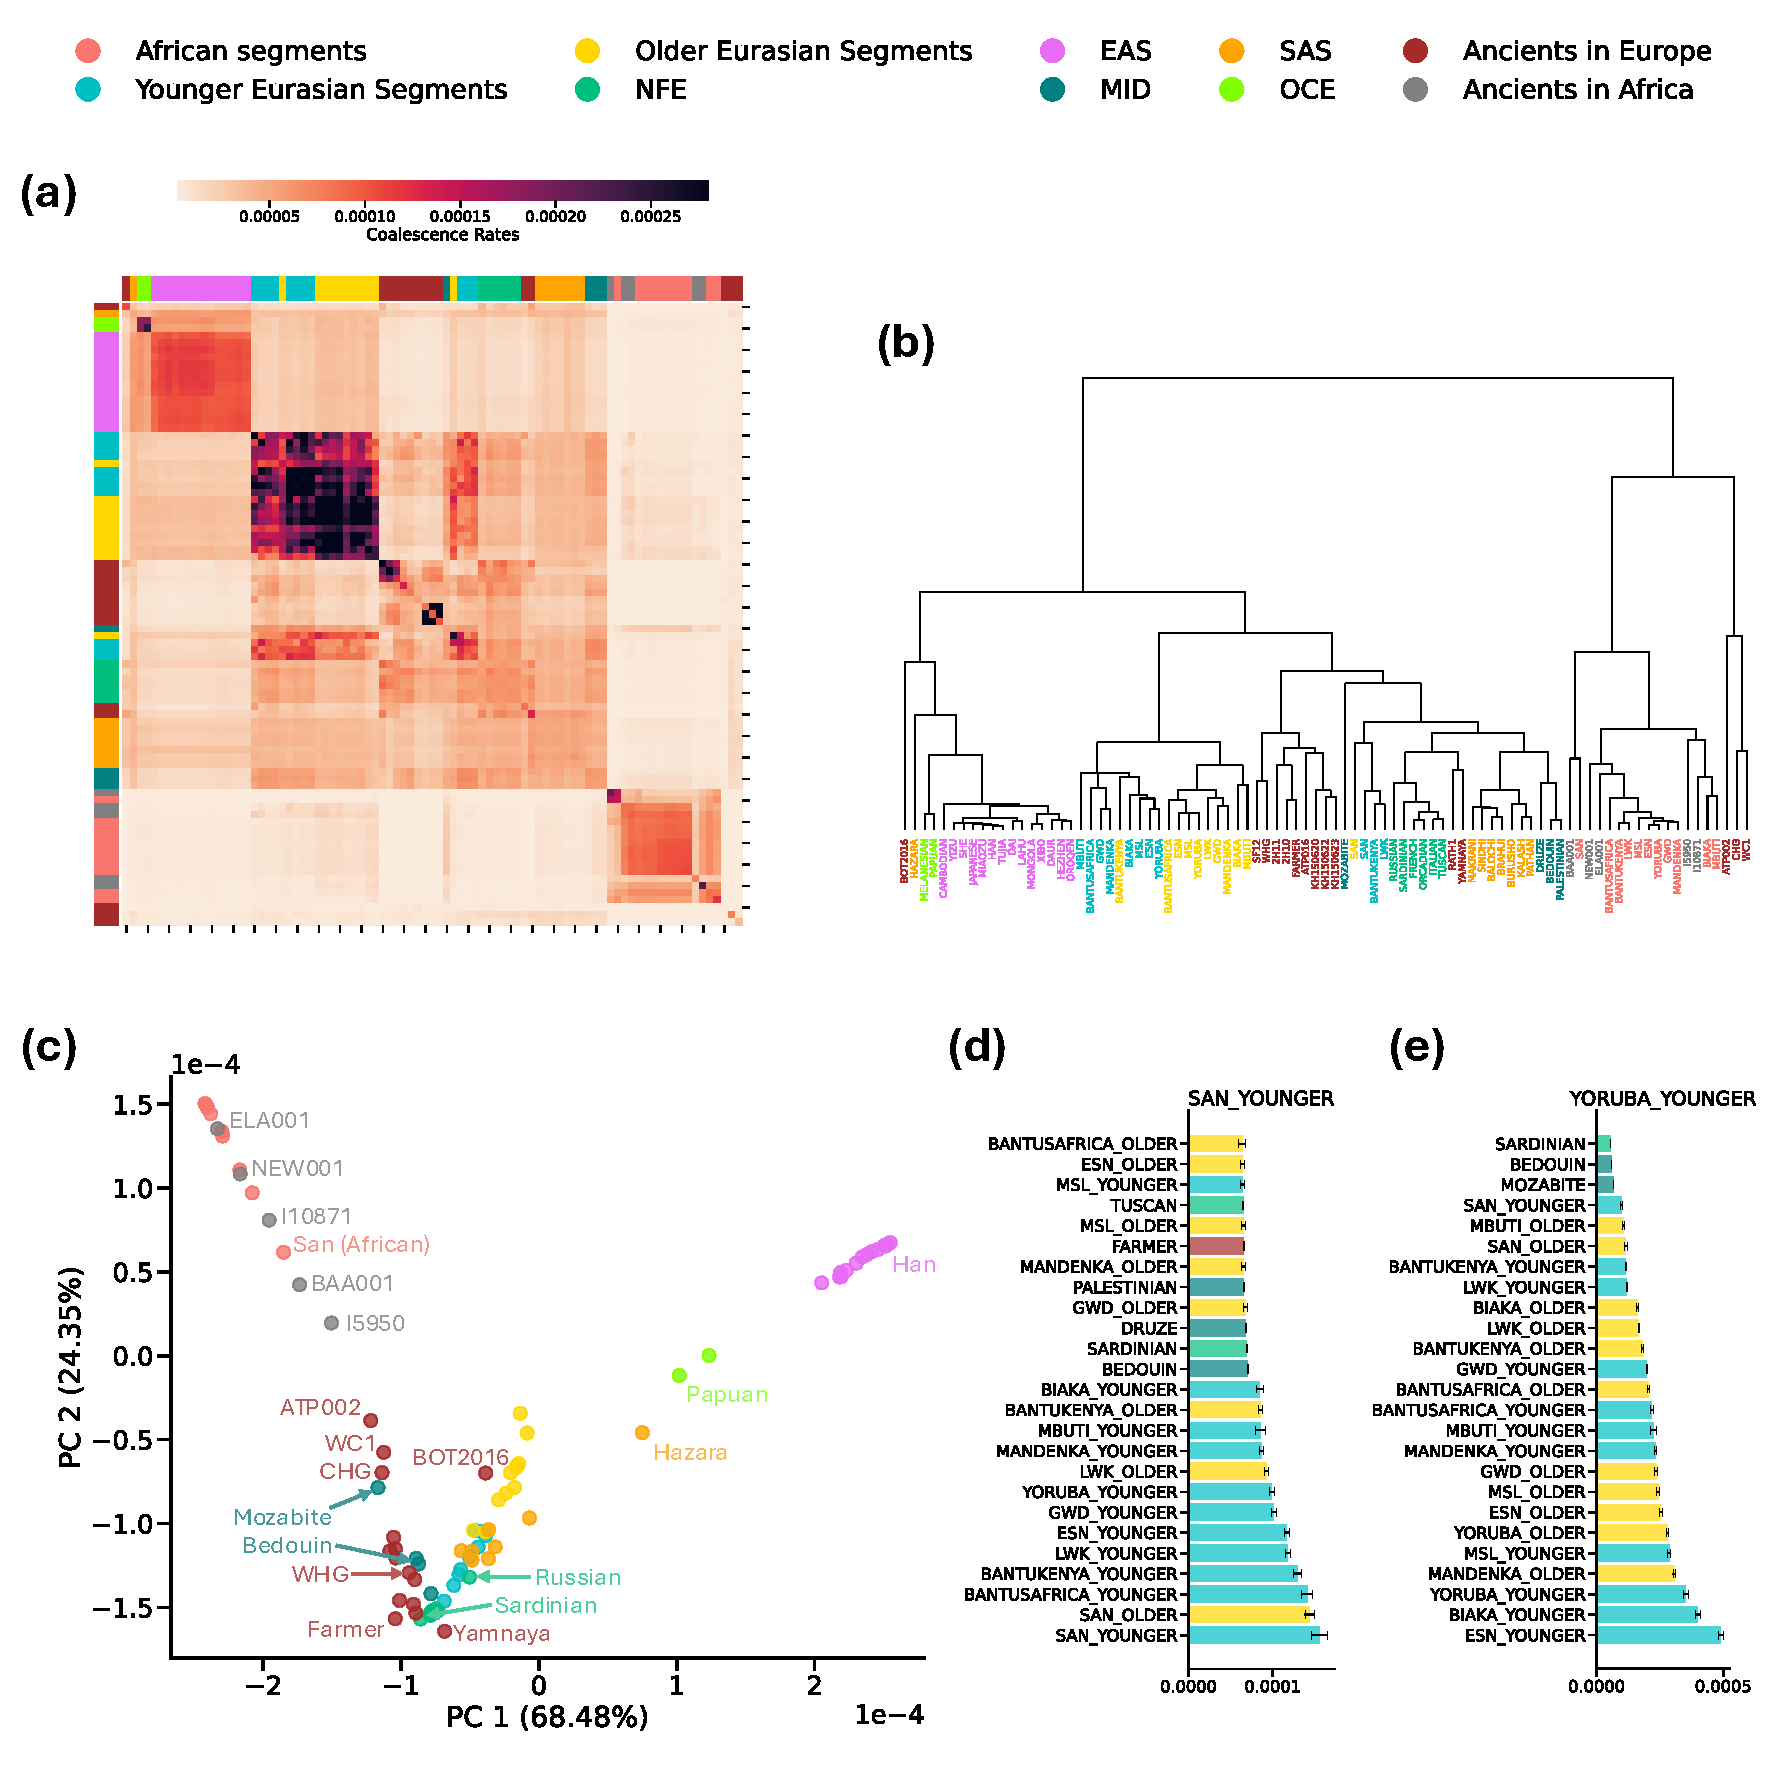
\includegraphics[width=\linewidth]{figures/gb_bta/gb_real_bta_12.pdf}
    \captionsetup{width=\textwidth+3cm}
    \caption{
    \footnotesize
    \textbf{Coalescence rates with modern and ancient samples.} (a) Matrix of pairwise coalescence rates for all modern and ancient groups in the epoch spanning $10{,}000$–$15{,}848$ years. (b) Dendrogram corresponding to the UPGMA hierarchical clustering of the pairwise coalescence rate matrix in (a). (c) PCA visualization of coalescence rates for the epoch spanning $10{,}000$–$15{,}848$ years, with PC1 and PC2 representing the eigenvectors capturing the greatest variance among modern samples. (d-e) Top $25$ groups based on coalescence rates with (d) younger Eurasian-like segments in the San, and (e) younger Eurasian-like segments in Yoruba during the epoch spanning $10{,}000$–$15{,}848$ years. Row and column colors in (a), dendrogram leaves in (b), and dots and bars in (c-e) are colored according to the common legend. NFE = non-Finnish Europeans, EAS = East Asians, MID = Middle Easterners and North Africans, SAS = South Asians, OCE = Oceanians. The numbers in brackets in (c) indicate the proportion of variance explained by each principal component. The error bars in (d-e) represent 95\% confidence intervals calculated using $100$ bootstraps. Results derived from HGDP+$1{,}000$GP+aDNA+archaic genealogies.
    }
\label{fig:gb-bta-source}
\end{figure}

\clearpage

% In order to characterize the admixture event further
% only focus on recent event
% We use the genealogies with moderns and ancients and calculate coal. rates given our local ancestry
% Do it seperately per population

%% Coal. rate epoch for moderns 0-10kya, for ancients 10kya-20kya
%% insert another figure with map with proportions, dates and source group per population - for younger admixture event only

% \subsection{Signatures of adaptive introgression}

% Admixture introduces new alleles into a population, some of which may be beneficial. This often manifests as an excess of one ancestry type at loci under selection. Using the local ancestry inferred with GhostBuster, we derive a selection statistic to measure the excess of Eurasian ancestry within African genomes, focusing specifically on ancestry from the younger admixture event. We define the selection statistic at each site based on the average Eurasian ancestry across all African samples in the HGDP+$1{,}000$GP dataset. To model this, we fit a beta-binomial distribution to the average Eurasian ancestry across sites, allowing for genetic drift, which can cause ancestry proportions to vary along the genome. Finally, we calculate p-values for excess Eurasian ancestry at each site based on the fitted beta-binomial distribution.

% We analyzed $270{,}000$ locations along the genome, excluding regions within or 50 kb around ENCODE blacklist regions \cite{amemiya2019encode}. The ENCODE blacklist identifies problematic genomic regions prone to artifacts in high-throughput sequencing, often due to excessive repeats, satellite sequences, or other anomalies that can interfere with accurate analysis. 

\section{Evidence of a deep admixture event in Africans}
\label{sec:ch3-gb-deep}

% The existence of deep population structure in Africa has ignited considerable debate in recent years, with multiple theories proposed to explain this complex evolutionary history. One hypothesis suggests the presence of ghost populations -- especially in regions of West Africa \cite{durvasula2020recovering}. Another theory, known as the “weakly structured stem” model, proposes the existence of multiple ancient populations more than $100{,}000$ years ago, which subsequently merged in varying proportions to form present-day African populations \cite{ragsdale2023weakly}. A third perspective highlights the role of gradual, continuous migration across populations, suggesting that African populations became blends of diverse ancestral groups \cite{lipson2020ancient}.

We used GhostBuster to understand the deep evolutionary history in Africa. Our analysis incorporates the same set of modern and ancient African samples as used in the ``Back-to-Africa'' section, detailed in Table \ref{tab:african_populations}. 

\subsection{Ancient admixture across sub-Saharan African populations}

To examine ancient events, we focused on coalescence events that occurred between $10{,}000$ and $5{,}000{,}000$ years ago, dividing this time frame into 20 epochs on a logarithmic scale. We excluded coalescence events more recent than $10{,}000$ years, as these likely represent more recent events like previously discussed back-to-Africa migrations. Consistent with previous analyses of back-to-Africa migration, we grouped non-Finnish Europeans (NFE), East Asians (EAS), and South Asians (SAS) as Eurasians. For each African population, analyses were conducted using all Eurasian and African populations in the dataset as reference groups, while excluding Middle Eastern and American populations from the reference panel. To further concentrate on broader lineage relationships, coalescence events between individuals within the target population were excluded. 
%To control for confounding effects due to back-to-Africa migration, we masked both the younger and older back-to-Africa segments, as identified in section \ref{sec:ch3-gb-bta}, from the local ancestry estimates.

Starting from a random initialization, the coalescence rates converged to reveal two distinct components. Figure \ref{fig:gb_deepadmix_1}a shows the inferred coalescence rates in Yorubans, used as a representative group. These rates suggest two components that primarily differ in their coalescence rates with Eurasians. We refer to the component closer to Eurasian populations as the out-of-Africa-like (OOA-like) component and the one relatively closer to African populations as the non-out-of-Africa-like (non-OOA-like) component. The Eurasian-like ancestry previously identified in Section \ref{sec:ch3-gb-bta} strongly correlates with the OOA-like component in this deep admixture, with more than $98$\% of segments attributed Eurasian-like lying within this component. This correlation is largely explained by the component's faster coalescence rate with Eurasians and supports the presence of two distinct types of Eurasian ancestries in Africans, as discussed in Section \ref{sec:ch3-gb-bta}. To specifically examine this deeper admixture events, we masked regions corresponding to previously identified Eurasian-like segments (posterior probability Eurasian-like > 10\%) and a $100$kb flanking region around them to avoid biases from recent back-to-Africa migration.

Both the held-out likelihood and the expected coefficient of determination indicate that two components best capture the observed coalescence differences without ambiguity regarding the admixture event (see Figure \ref{fig:gb_deepadmix_1}b and Figure \ref{fig:gb_deepadmix_cv_all}). We identified varying proportions of OOA-like and non-OOA-like components across modern and ancient African groups after removing ancestry corresponding to the back-to-Africa migration. Among modern groups in the HGDP+$1{,}000$GP and SGDP datasets, Dinka individuals exhibited the highest proportion of OOA-like ancestry at approximately $36.8$\%, while Khomani San individuals showed the lowest at $10.6$\%. In ancient individuals, we detected $35.9\%$ OOA-like ancestry in the $4{,}500$-year-old Mota individual, $27.6\%$ in a $7{,}900$-year-old ancient African from Cameroon, and $30.1\%$ in younger ancient samples from South Africa, namely ela001 and new001. In contrast, the Ballito Bay individual, baa001, exhibited $12.3\%$ OOA-like ancestry. Overall, we observed a higher proportion of the OOA-like component in East Africa, followed by West and South Africa, with the lowest levels in Central African hunter-gatherers (see Figure \ref{fig:gb_deepadmix_1}d). The first four principal components of the coalescence count and opportunity matrix did not reveal substantial differences between clusters (see Figure \ref{fig:gb_deepadmix_1}b). This is attributable to the large number of African reference panel groups compared to a single group representing Eurasians, which exhibit less variation between the components inferred by GhostBuster.

\begin{figure}[h!]
    \centering
    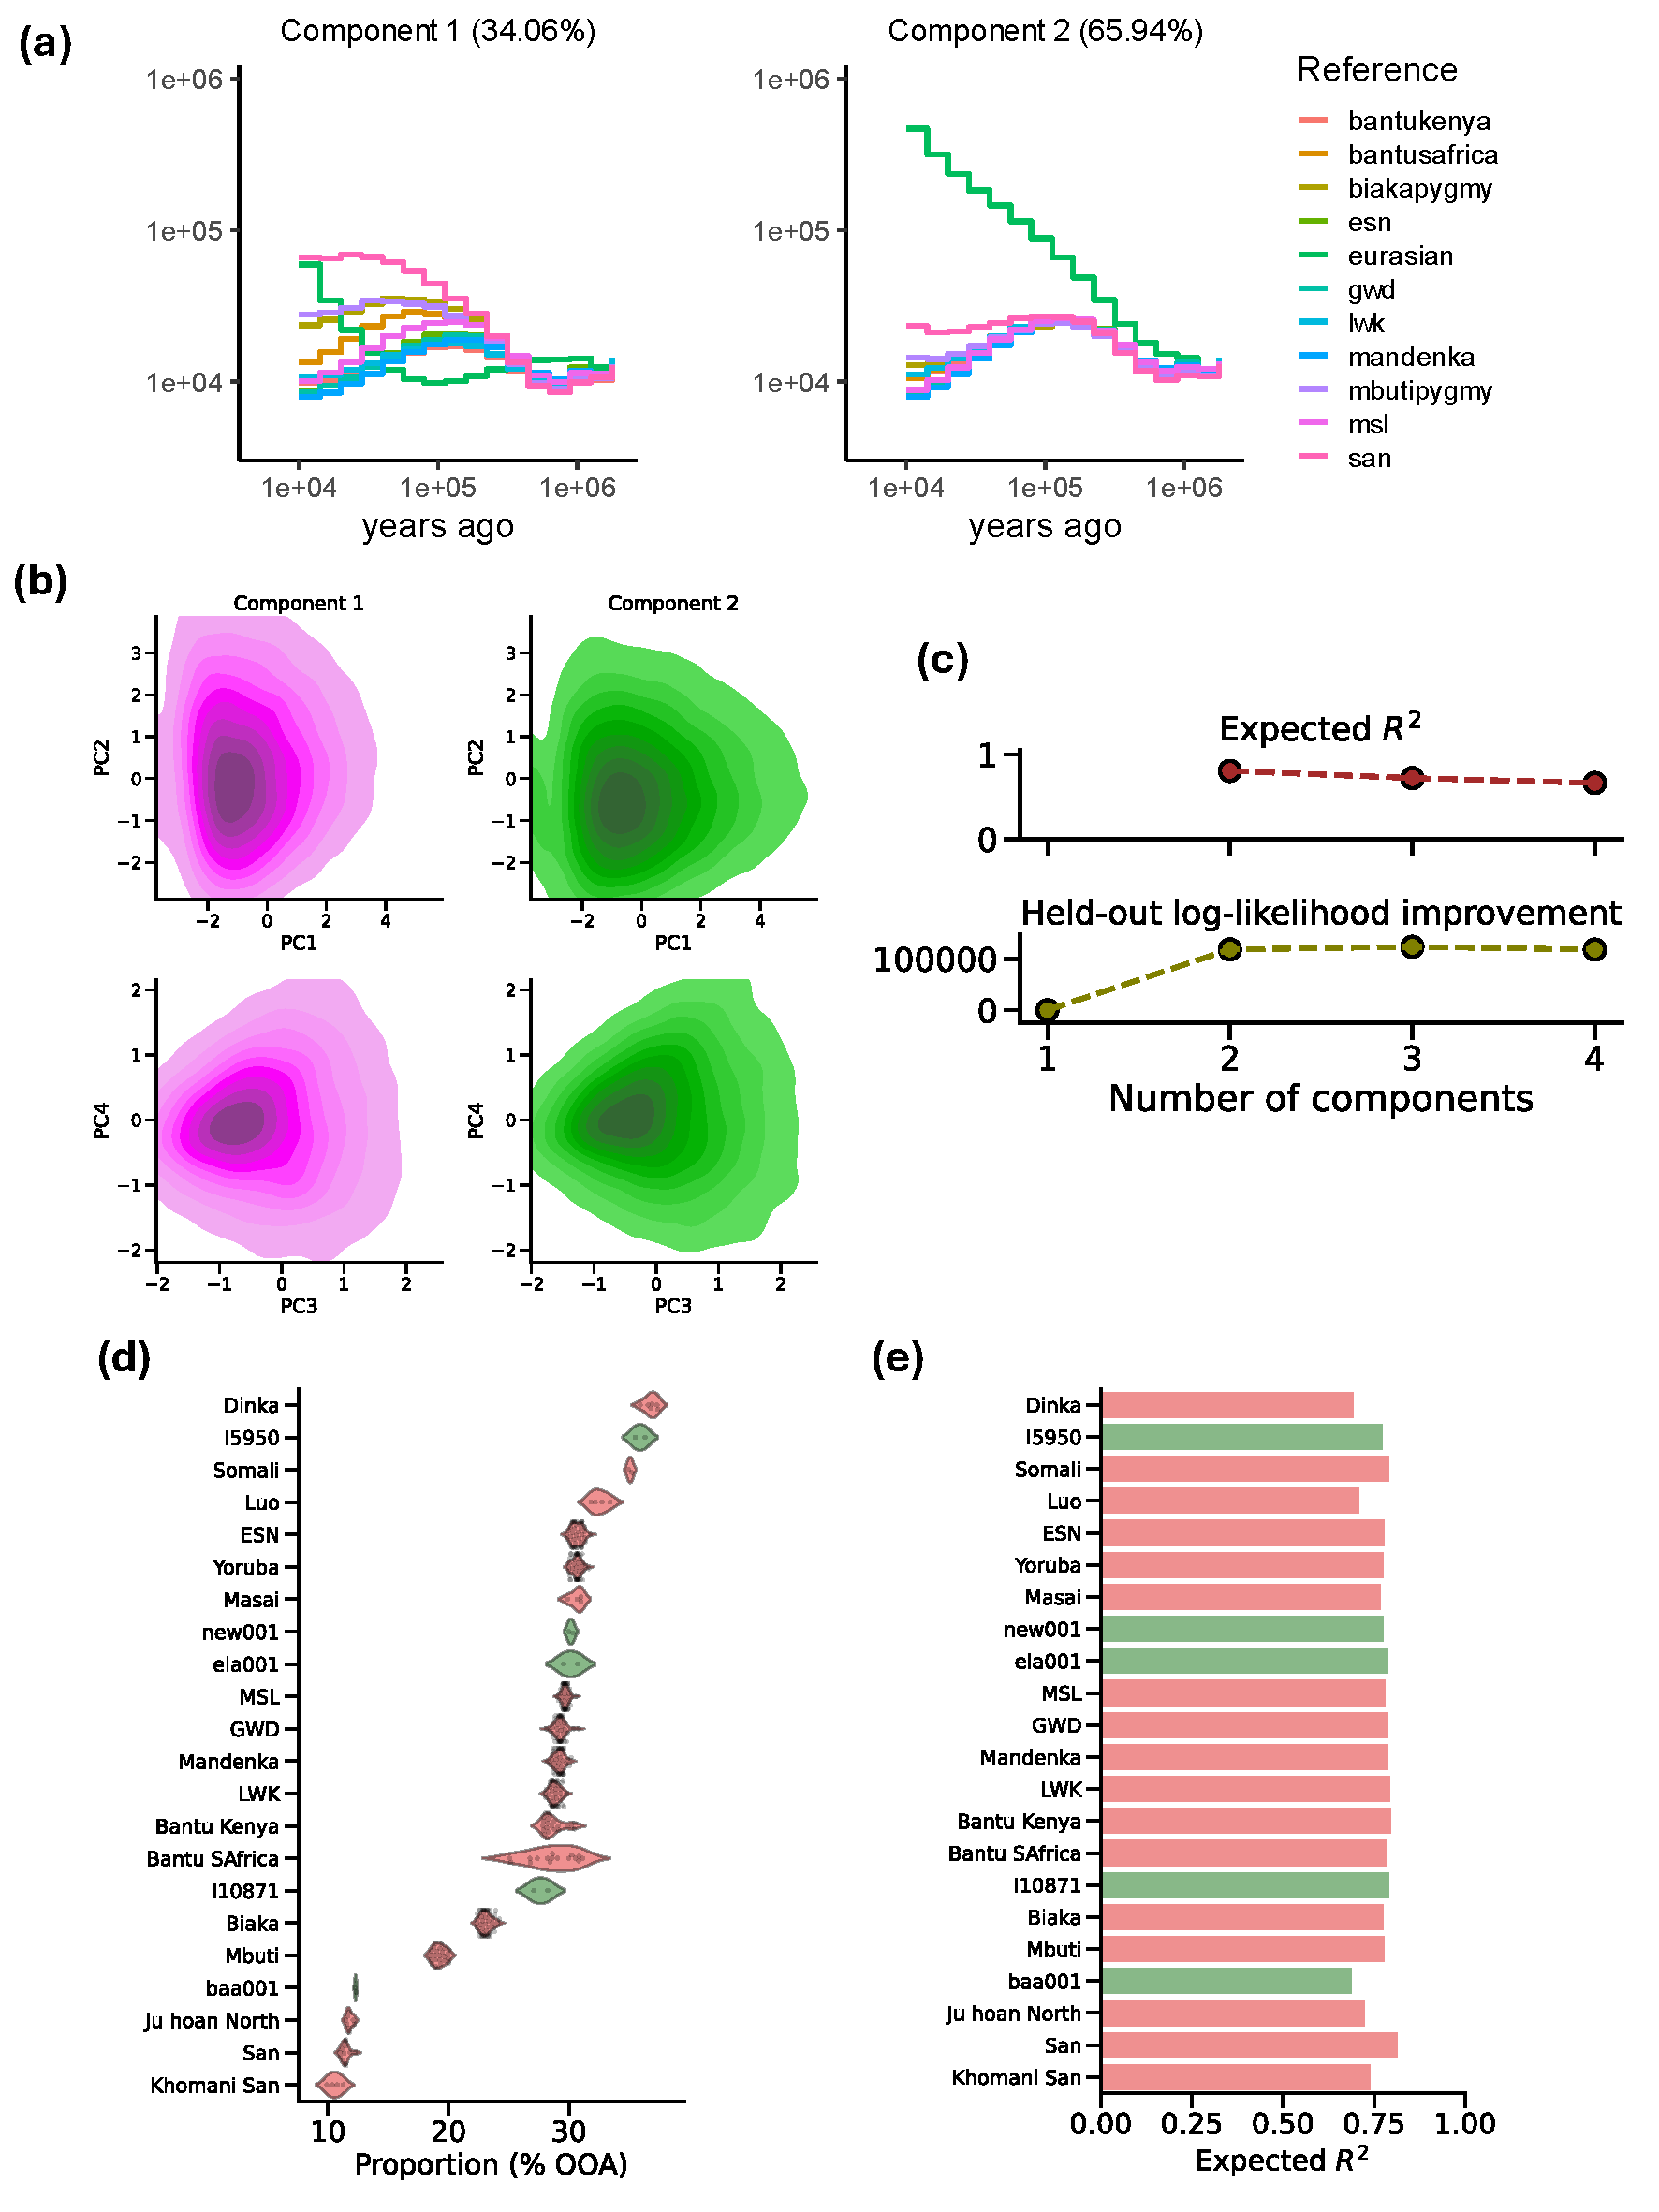
\includegraphics[width=\linewidth]{figures/gb_deepadmix/gb_real_deep_1.pdf}
    \captionsetup{width=\textwidth+3cm}
    \caption{
    \footnotesize
    \textbf{Decomposing sub-Saharan Africans to find a deep admixture event.} (a) Inferred inverse coalescence rates and proportions when decomposing Yorubans: each line represents inverse coalescence rate profiles with a reference population. (b) PCA visualization of the coalescence count and opportunity matrix derived from the genealogies plotted separately for each component. (c) Expected coefficient of determination and held-out log-likelihood improvement with varying number of components. (d) Proportion of the out of Africa-like ancestry and (e) Expected coefficient of determination across all African populations analyzed. The PCA visualization in (b) is based on a KDE plot with a threshold of 0.05, and binary local ancestry estimates are obtained by thresholding the inferred posteriors at 0.5. Individual data-points overlaid on the violin plots. 
    }
    \label{fig:gb_deepadmix_1}
\end{figure}

\clearpage

\subsection{Dating the admixture event}

We constructed coancestry curves using the inferred local ancestry data without filtering out previously identified back-to-Africa segments. These curves were then used to fit various admixture dating models, including single-date, two-date, and continuous admixture models. Similar to the back-to-Africa migration, we found that a single-date model did not provide a good fit to the coancestry curves. Notably, the two-date admixture model provided the best fit for the coancestry data across 10 out of 16 African populations (see Figure \ref{fig:gb_deepadmix_3}). Consistent with the back-to-Africa migration, the younger admixture dates ranged from $1{,}500$ to $7{,}000$ years ago, while the older admixture event occurred approximately $23{,}000$ to $40{,}000$ years ago (see Figure \ref{fig:gb_deepadmix_3}).

Next, we removed the local ancestry in and around the Eurasian-like segments previously identified in Section \ref{sec:ch3-gb-bta} and recalculated the coancestry curves. After removing the local ancestry corresponding to the more recent back-to-Africa migration, we found that the single-date admixture model fit the coancestry data as well as the two-date and continuous admixture models in most scenarios (see Figure \ref{fig:gb_real_deep_dating_wobta}). This suggests that the younger date in the initial fit most likely captures the more recent back-to-Africa migration. Therefore, we focus on the older date as the estimated time of admixture between OOA-like and non-OOA-like populations and exclude the Eurasian-like ancestry identified in the back-to-Africa section from all subsequent analyses. This admixture is dated to  $23{,}000$-$40{,}000$ years across groups (see Table \ref{tab:gb_deep_admix_dates}). It is important to note that these admixture dates have not been adjusted for potential errors in the recombination map, as we lacked reliable error estimates for it. We believe this may introduce a downward bias in the dating estimates \cite{sankararaman2012date}. However, it might be reasonable to assume that the admixture occurred around or after the out-of-Africa migration dated around $50{,}000$–$100{,}000$ years ago \cite{lopez2015human}. 

Given the deep nature of the admixture, we performed additional ``sanity checks'', such as running GhostBuster with the HMM disabled and using only African reference populations (removing Eurasians). These analyses produced similar coalescence rates and correlated but more uncertain local ancestry estimates compared to the initial run with the HMM enabled and Eurasian samples included in the reference population (see Figure \ref{fig:gb_deepadmix_sanity1} and \ref{fig:gb_deepadmix_sanity2}).

\begin{figure}[h!]
    \centering
    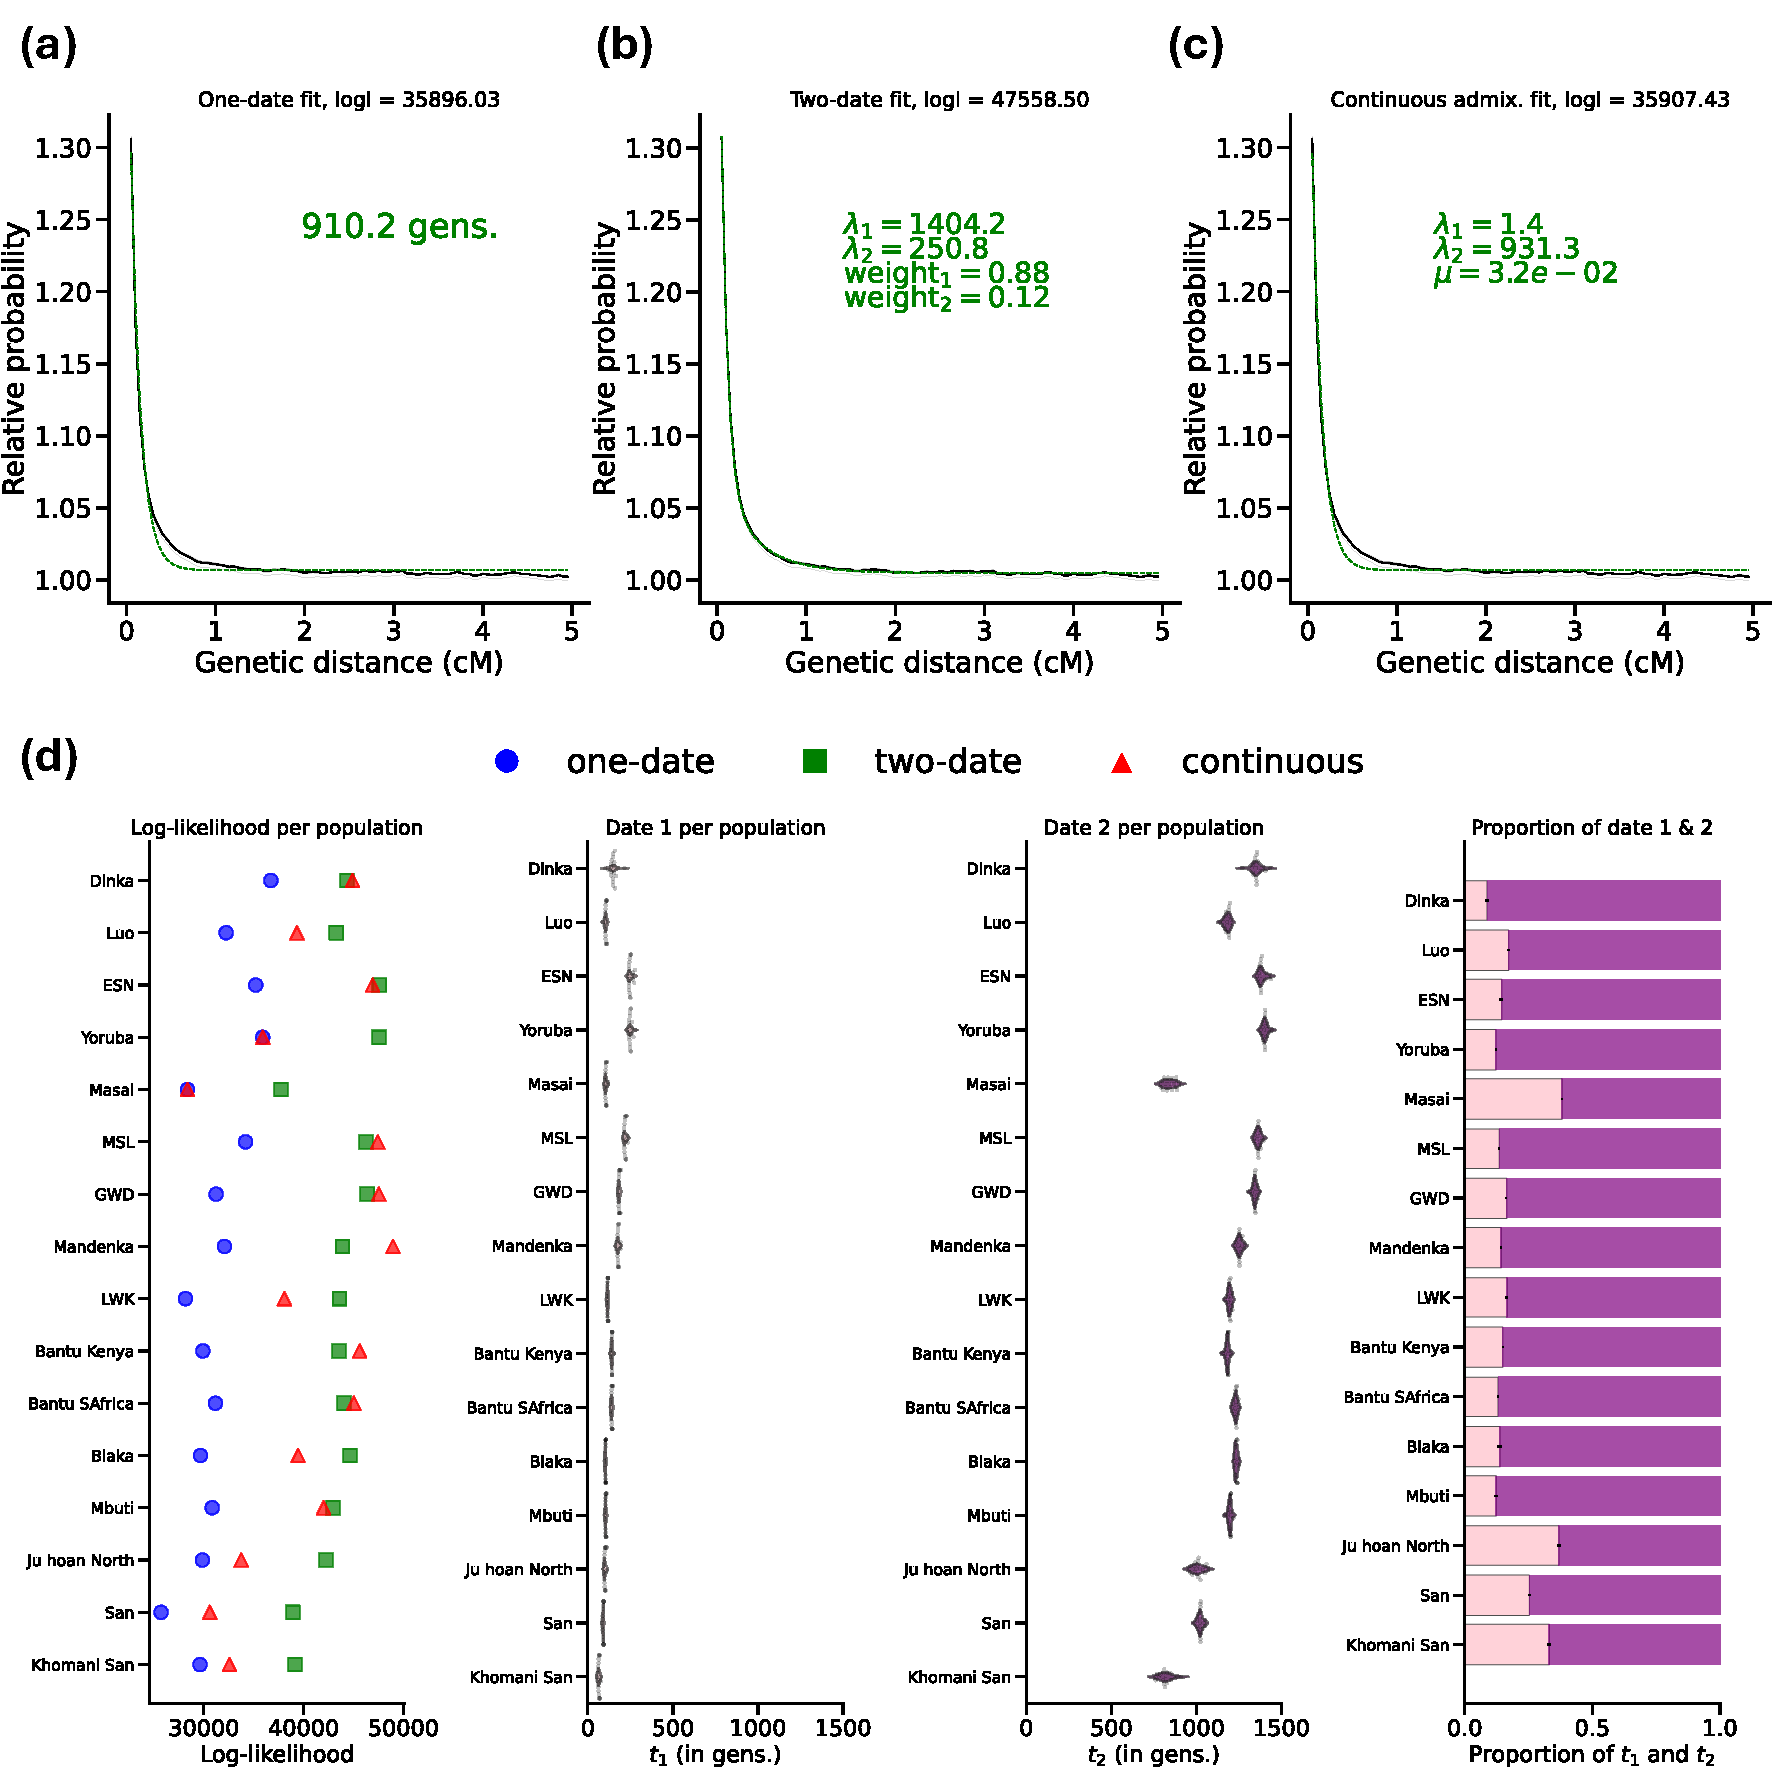
\includegraphics[width=\linewidth]{figures/gb_deepadmix/gb_real_deep_3.pdf}
    \captionsetup{width=\textwidth+3cm}
    \caption{
    \footnotesize
    \textbf{Dating the ancestral components corresponding to deep admixture event.} Coancestry curves and (a) one-date admixture model fit, (b) two-date admixture model fit and (c) constant migration rate continuous admixture model fit for Yorubans. (d) Per-population least squared log-likelihood corresponding to various admixture models along with the admixture dates and weights inferred using two-date admixture model. The log-likelihood values are aggregated across $20$ jackknife runs. Populations are sorted based on highest to lowest proportion of Eurasian-like ancestry, pink represents the younger admixture date and purple represents the older admixture date in (d). Individual data-points overlaid on the violin plots. Admixture dates in the plot are in generations.
    }
    \label{fig:gb_deepadmix_3}
\end{figure}

\clearpage

\subsection{Mutational profiles validate the admixture event}
\label{sec:ch3-gb-deep-mut}

We used mutation profiles as near orthogonal evidence that GhostBuster has identified two distinct components that are unlikely to be data or method artefacts. Similar to the analysis in Section \ref{sec:ch3-gb-bta-mutational}, we calculated the normalized mutational enrichment profiles for continental populations and inferred mixture components relative to genome-wide normalized mutation rates in the African population.

In contrast to our analysis of the more recent back-to-Africa migration, we did not observe enrichment for TCC to TTC mutations (see Figure~\ref{fig:gb-mutational-all-deep}). This is likely because this admixture event predates the emergence of TCC to TTC mutations in Eurasian populations. However, we detected distinct patterns in the enrichment of weak to strong mutations between the two ancestry components. To classify mutations as weak or strong, CpG sites were excluded, following the approach used in analyzing the back-to-Africa migration. We observed a reduction of weak to strong mutations in the out-of-Africa-like (OOA-like) component compared to genome-wide weak to strong mutation rates within Africa. This reduction peaked approximately $50{,}000$ -- $100{,}000$ years ago, aligning with patterns observed in other Eurasian populations (see Figure \ref{fig:gb-mut-ws-deep}a-b). These findings suggest a notable divergence in the trajectories of existing mutations during this period, driven by differential GC-biased gene conversion between the two ancestral components. Among ancient samples, the $4{,}500$-year-old individual from Mota Cave (I5950) and the $400$-year-old individual from South Africa (new001) exhibited approximately double the weak-to-strong mutation reduction signal compared to modern samples (see Figure \ref{fig:gb-mut-ws-deep}c). This increase cannot be attributed to our estimated uncertainty and may suggest that the OOA-like group ancestors for these individuals experienced a particularly small effective population size. In contrast, the $1{,}900$- and $500$-year-old individuals from South Africa (baa001 and ela001) displayed a subtle weak-to-strong signal reduction in the OOA-like group, similar to what is observed in modern-day samples (see Figure \ref{fig:gb-mut-ws-deep}c). Meanwhile, the $7{,}900$-year-old individual from Cameroon (I10871) showed no significant difference in weak-to-strong enrichment between the two components (see Figure \ref{fig:gb-mut-ws-deep}c).

\begin{figure}
    \centering
    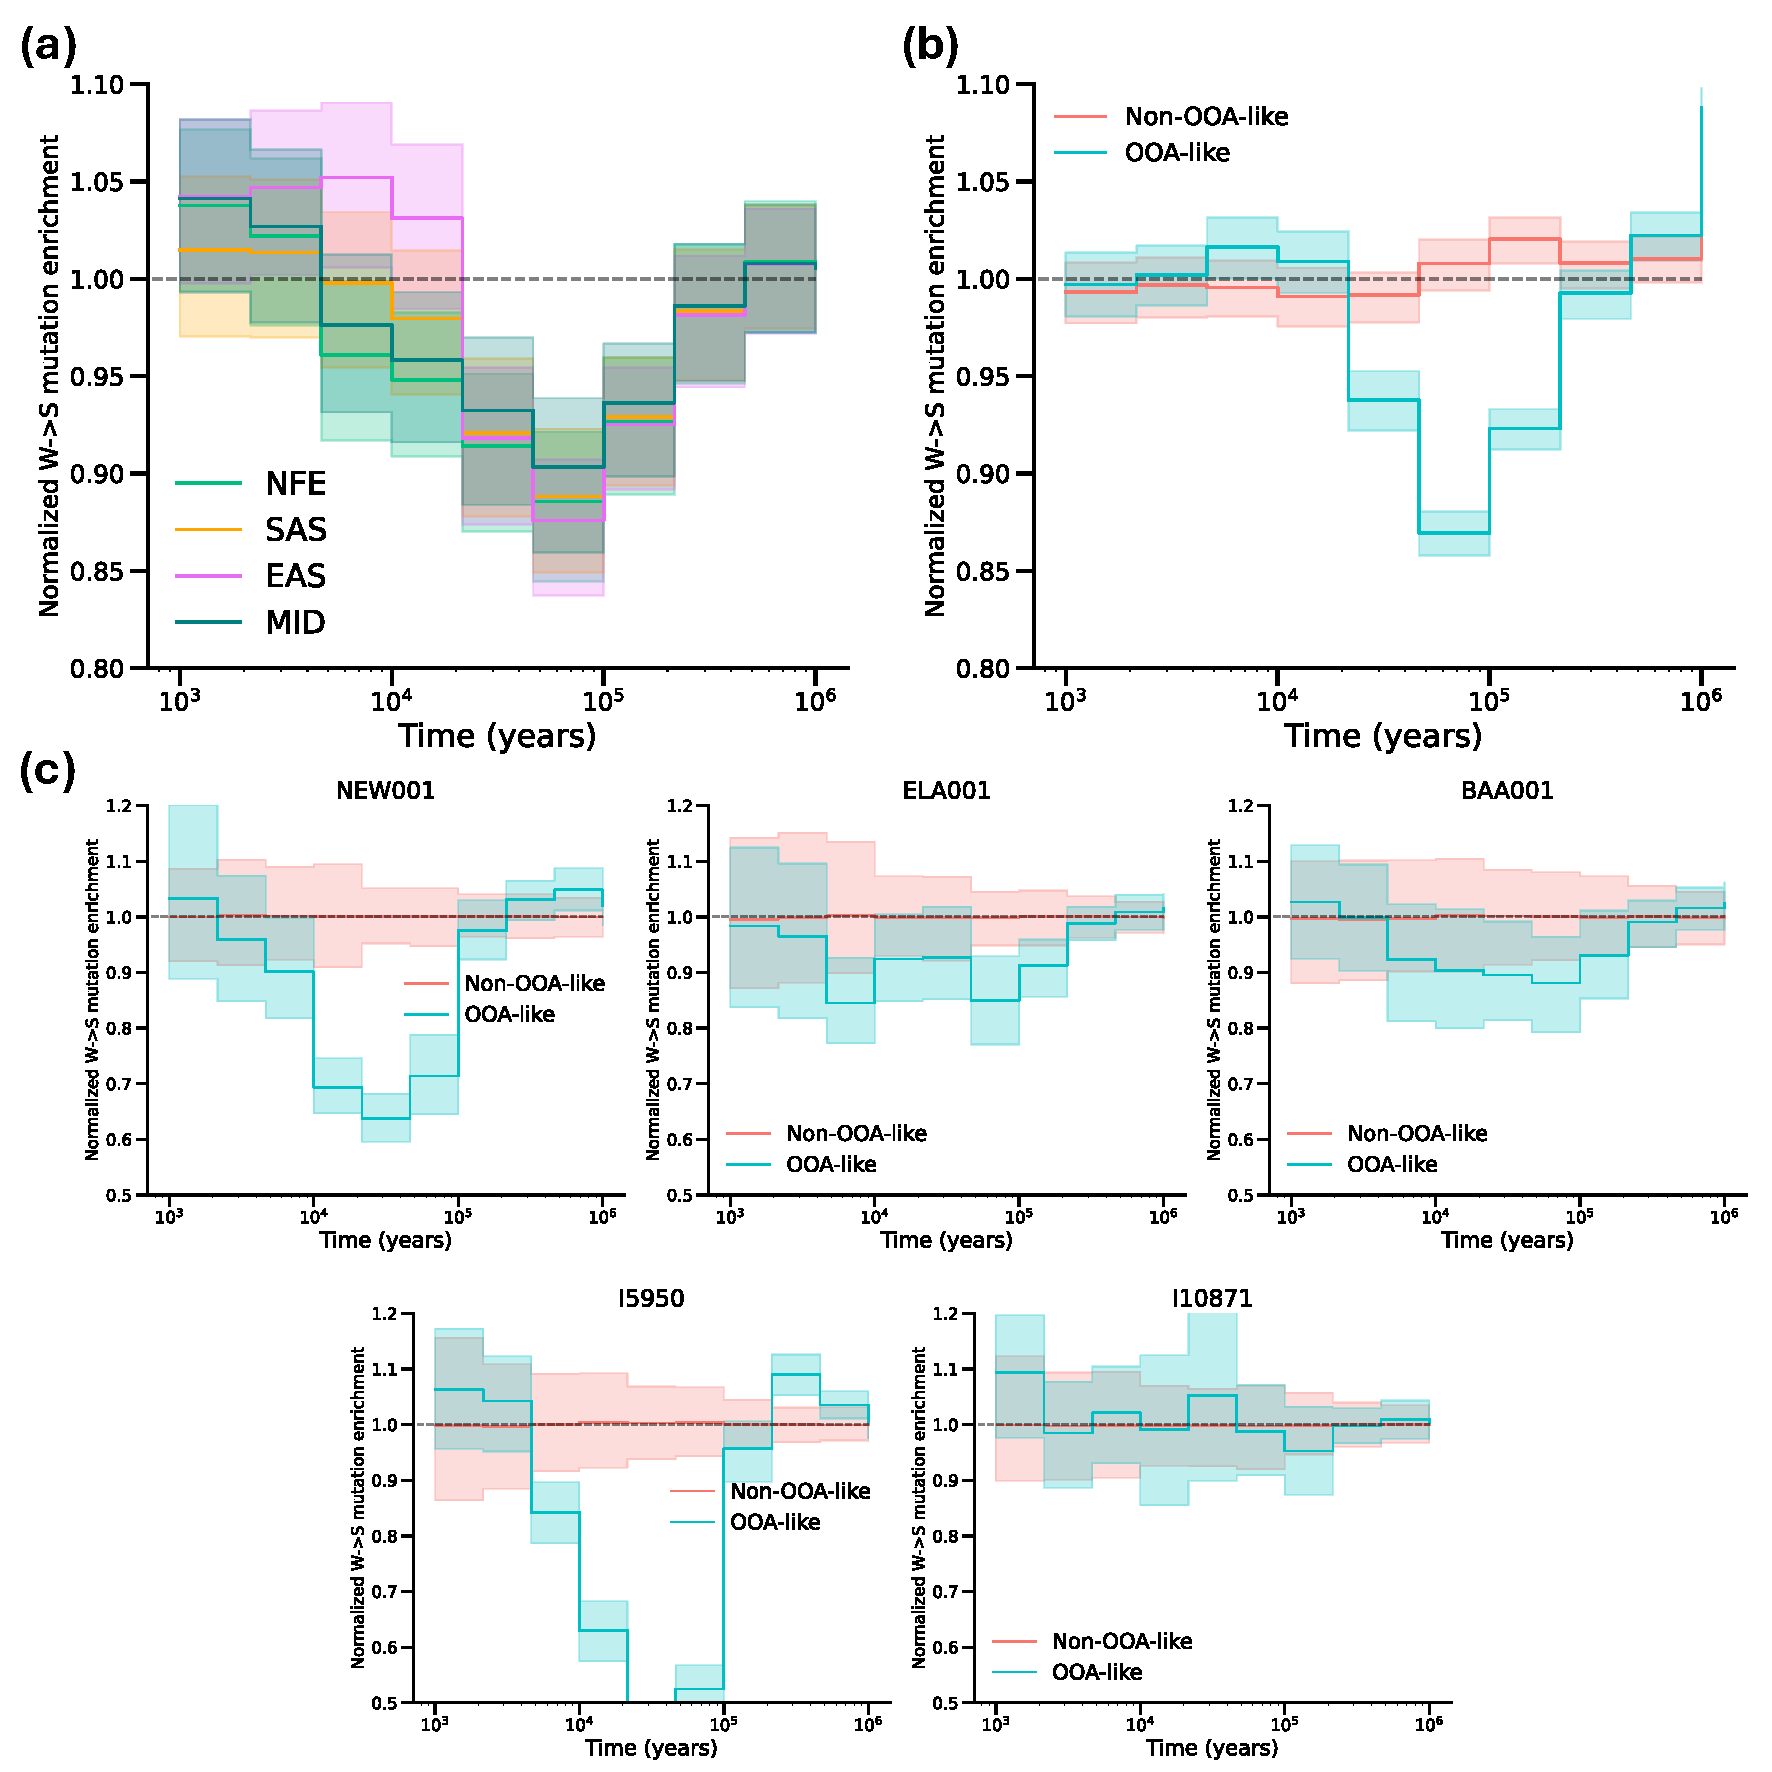
\includegraphics[width=\linewidth]{figures/gb_deepadmix/gb_real_deep_8.pdf}
    \captionsetup{width=\textwidth+3cm}
    \caption{
    \footnotesize
    \textbf{Enrichment of weak to strong mutation rates in the deep admixture African components.} (a) Enrichment of weak to strong mutation rates across various continental groups, including NFE (non-Finnish Europeans), SAS (South Asians), EAS (East Asians), and MID (Middle Eastern and North African populations). (b) Enrichment of weak to strong mutation rates in OOA-like and non-OOA-like (African) segments in African populations. (c) Weak to strong mutation rate enrichment in five ancient African samples, including new001, ela001, baa001, I5950, and I10871 (see population descriptions in Table \ref{tab:african_populations_2}). Shaded regions indicate 95\% confidence intervals derived from $1{,}000$ bootstrap replicates, while the dashed line represents the baseline of no enrichment. Results derived from HGDP+$1{,}000$GP and HGDP+$1{,}000$GP+aDNA+archaic genealogies.
    }
\label{fig:gb-mut-ws-deep}
\end{figure}

\clearpage

\subsection{Variation in PRDM9 activity across populations}
In humans, recombination predominantly occurs at specific regions in the genome known as recombination hotspots. The placement of these hotspots is largely governed by the PRDM9 gene, which encodes a zinc finger protein responsible for identifying and binding to distinct DNA sequence motifs. Once bound, PRDM9 modifies histones near the binding sites, creating an environment conducive to recombination initiation.

Multiple types of PRDM9 have been identified in humans, distinguished by variations in the zinc finger array configuration. These PRDM9 types can bind to different sequence motifs across the genome, resulting in distinct recombination hotspot locations. Of all the known PRDM9 types in humans, PRDM9-A is the most common, binding to a specific sequence motif (``CCNCCNTNNCCNC'') \cite{coop2008high,myers2008common}. It is present in all modern human populations but absent in chimpanzees \cite{myers2010drive}. PRDM9-B shares most of its binding motif with PRDM9-A and thus targets similar hotspot locations. Another notable PRDM9 type, PRDM9-C, binds to a distinct sequence motif, a unique 17-base pair sequence (``CCgCNgtNNNCgtNNCC''), which directs recombination events to different genomic locations. The small letters in the motif indicate less conserved bases. PRDM9-C is particularly common in African populations but occurs less frequently in Eurasian populations \cite{hinch2011landscape,wegmann2011recombination,alleva2021cataloging}. Importantly, the probability of crossover hotspots associated with PRDM9-C is strongly influenced by the alleles an individual carries at the PRDM9 gene (rs6889665, $p<10^{-245}$ \cite{hinch2011landscape}). 

The recombination machinery repairs double-strand breaks with a slight preference for incorporating GC alleles over AT alleles, leading to GC-biased gene conversion and an increased rate of weak to strong mutations around recombination hotspots. Separately, frequent DNA repair at these hotspots gradually erodes the sequence motifs that PRDM9 zinc fingers bind to, a phenomenon known as hotspot death. The continual loss of hotspots places evolutionary pressure on PRDM9 to form new hotspots through alterations in its zinc finger domains, changing its binding specificity. Consequently, PRDM9 has become one of the fastest-evolving genes, constantly adapting to balance hotspot erosion and renewal \cite{myers2010drive,baker2017repeated}. While the locations of recombination hotspots are determined by the specific PRDM9 allele an individual carries, examining GC-biased gene conversion and signatures of hotspot death at these sites provides insight into the evolutionary history of a lineage. We leverage this evolutionary information to improve our understanding and provide independent evidence of the ancient admixture event under investigation.

We begin by examining the PRDM9-C allele (rs6889665), which has previously been shown to strongly predict the probability of crossover at PRDM9-C hotspots \cite{hinch2011landscape}. In our dataset, we found the SNP rs6889665 to have a frequency of $33.7\%$ in Africans, $8.4\%$ in East Asians, $7.4\%$ in South Asians, and $6.3\%$ in non-Finnish Europeans. Additionally, its frequency was $44.1\%$ in the non-out-of-Africa (non-OOA-like) component but only $2.7\%$ in the out-of-Africa-like (OOA-like) component. Figure \ref{fig:gb_deep_prdm9c_tree} depicts the tree at PRDM9, identifying rs6889665 as one of the oldest mutations on the tree. Notably, the mutation shows an excess of descendants inferred to possess ancestry from the non-OOA-like component compared to the OOA-like component.

Next, we analyzed the PRDM9-A and PRDM9-C hotspots along the genome (provided by Dr. Anjali Hinch) to investigate differences in their evolutionary histories across various populations and ancestral components involved in the deep admixture event. Specifically, we examined weak to strong mutations in and around these hotspots and their impact on different populations. PRDM9-A and PRDM9-C hotspots were analyzed separately, excluding regions where both hotspots occur within a 5kb interval. Consistent with the mutational enrichment analysis, CpG sites were excluded when classifying mutations as weak or strong. 

To understand population-level differences in PRDM9 activity, we began by examining the number of descendants carrying the weak to strong mutations at these hotspots per population. This quantity was normalized by the total number of population samples in the dataset and the AT content of the region. Furthermore, we only considered mutations with an age of less than one million years. Figure \ref{fig:gb_deepadmix_prdm9_hotspot}a,c presents the normalized descendant count per continental population as a function of the distance from the hotspot center for weak to strong mutations. For hotspots associated with PRDM9-A, we observed similar peak intensities around the hotspot center across all continental populations analyzed. In contrast, PRDM9-C hotspots exhibited differences in activity across continental populations, with Africans showing a higher peak compared to non-African populations. This discrepancy could be attributable to population-specificity of PRDM9-C allele previously identified \cite{hinch2011landscape, alleva2021cataloging}.

To explore differences in weak to strong mutation rates across the ancestral components involved in the deep admixture event, we analyzed weak to strong mutations within $1{,}000$ bp of the hotspot center and calculated the time-stratified mutation rate enrichment as described in Section \ref{sec:ch3-gb-deep-mut}. However, it is important to note that while Relate provides estimates of mutational ages, its accuracy within hotspots is limited. These estimates are likely correlated with true ages, but they should not be interpreted as highly precise chronological markers. Unlike the genome-wide mutational enrichment analysis, we normalized the enrichment relative to the mutation rate in East Asians (rather than Africans) and focused exclusively on regions around the hotspots. 

Figure \ref{fig:gb_deepadmix_prdm9_hotspot}b,d illustrates the weak to strong mutation rate enrichment for the OOA-like and non-OOA-like components at PRDM9-A and PRDM-C hotspots respectively. Relative to the weak to strong mutation rate in East Asians, both the OOA-like and non-OOA-like components exhibited enrichment for weak to strong mutations around $50{,}000$ years ago at PRDM9-A hotspots. 
%
This enrichment was of a similar magnitude for both components. However, in regions near PRDM9-C hotspots, we observed a significant difference in enrichment between the two components (see Figure \ref{fig:gb_deepadmix_prdm9_hotspot}d), with the non-OOA-like component exhibiting higher weak to strong mutations. This suggests that the PRDM9-C allele historically exhibited greater activity relative to the PRDM9-A allele in the non-OOA-like group compared to the OOA-like group.
%
This finding, along with the broader differences in GC-biased gene conversion (GCbGC), provides compelling evidence that the two groups represent genuine, ancient population stratification within African ancestral groups. It is difficult to conceive of confounding factors that could misclassify ancestry in a way that would result in distinct mutation types appearing on separate lineages. This is particularly true given that information about mutation type is invisible to GhostBuster and that our normalization procedure for identifying mutational biases explicitly matches the genomic regions used to define OOA-like and non-OOA-like mutation profiles.
%
Furthermore, these patterns align precisely with a priori expectations of ancient stratification. The present-day frequency of PRDM9-C is lower than PRDM9-A in both non-African and inferred OOA-like African individuals, while it is comparatively higher in non-OOA-like African lineages. These observations strongly support the hypothesis of deep population structure within African ancestral groups.
% This enrichment was of a similar magnitude for both components. However, in regions around PRDM9-C hotspots, we observed differential enrichment between the two components, with the non-OOA-like component showing higher weak to strong mutation rates. This suggests that the PRDM9-C allele may have originated in the non-OOA-like population and was subsequently introduced into the OOA-like population through some sort of gene-flow. More importantly, the differential signals at PRDM9-C hotspots provide independent evidence that the structure we are identifying in Africa is likely real. 
Finally, it is worth noting that the mutation rate enrichments shown in Figure \ref{fig:gb_deepadmix_prdm9_hotspot}b,d are based on mutations mapped to the genealogy. A small fraction of mutations (less than $3$\%) do not map to the genealogy and therefore cannot be dated. Nevertheless, we believe the observed signal is robust and unlikely to be affected by these non-mapping mutations.

\begin{figure}[h!]
    \centering
    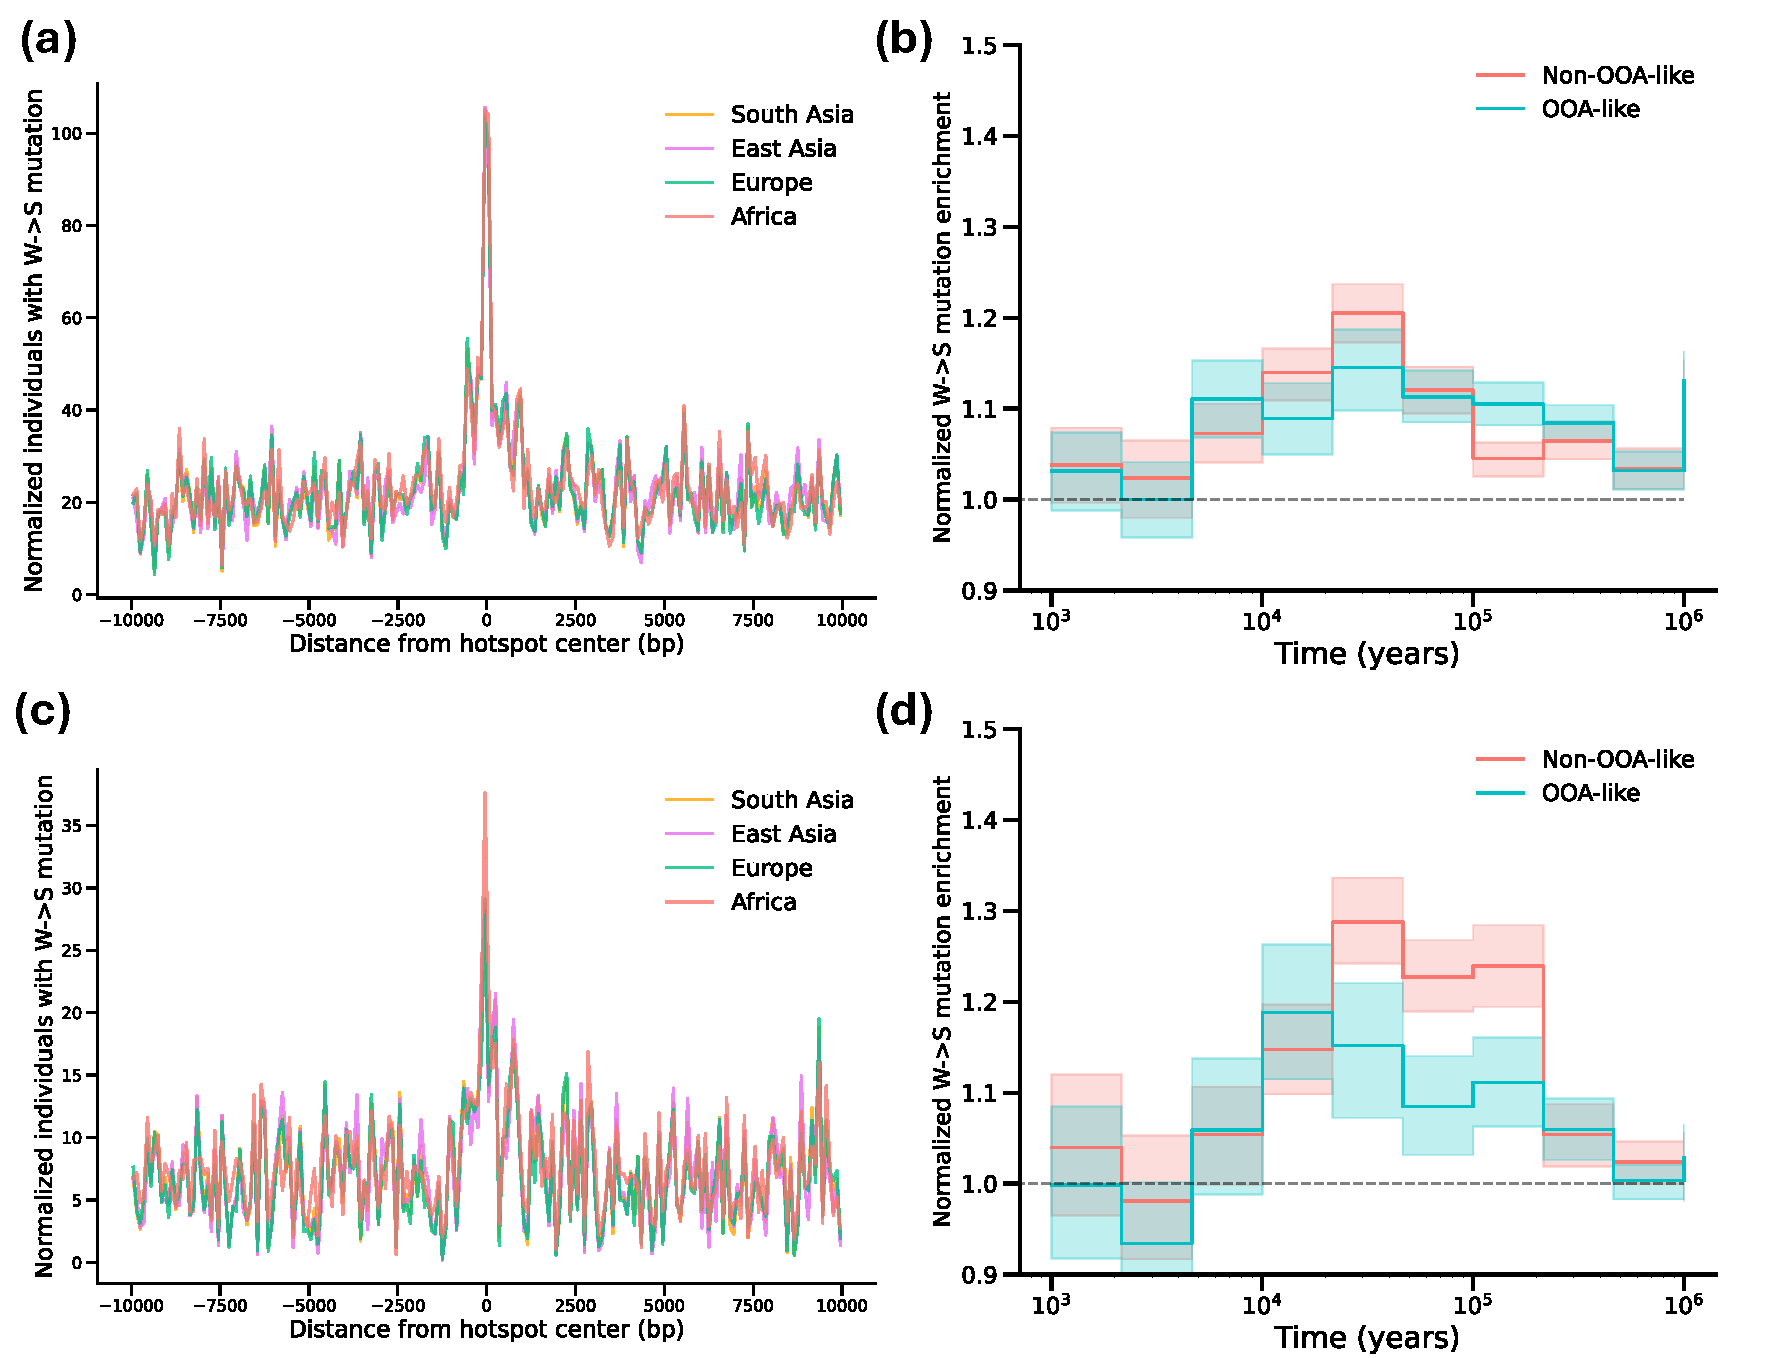
\includegraphics[width=\linewidth]{figures/gb_deepadmix/gb_real_deep_4.pdf}
    \captionsetup{width=\textwidth+3cm}
    \caption{
    \footnotesize
    \textbf{Weak to strong mutation rates at recombination hotspots across populations.} Weak to strong mutation counts across populations and deep admixture component in (a-b) PRDM9-A hotspots, (c-d) PRDM9-C hotspots. Panel (a) and (c) measure the number of individuals carrying weak to strong mutations around the PRDM9 hotspots, normalized by the total number of individuals and the AT content of the region. Whereas, Panel (b) and (d) measure the time-stratified normalized mutation rate enrichment with respect to weak to strong mutation rates in East Asians. In panel (b) and (d) the shaded regions indicate 95\% confidence intervals derived from $1{,}000$ bootstrap replicates, while the dashed line represents the baseline of no enrichment. Results derived from HGDP+$1{,}000$GP and HGDP+$1{,}000$GP+aDNA+archaic genealogies.
    }
    \label{fig:gb_deepadmix_prdm9_hotspot}
\end{figure}

\clearpage

\subsection{Characterizing the admixture event using coalescence rates}
%% split times 
%% Relation with Nea. and Denisovans
%% Relation with OOA population

In order to characterize the deep admixture event better, we look at the relationship of two ancestral components with various modern, ancient and archaic populations. Similar to analysis in Section \ref{sec:ch3-gb-bta-source} we calculate coalescence rates with modern samples from HGDP+$1{,}000$GP dataset and 49 high-coverage ancients and 4 archaic human groups (see Table \ref{tab:gb_ancient_samples}) conditioned on the inferred local ancestry for each African population. 

We consider coalescence events in epoch corresponding to $64{,}000$-$100{,}000$ years in the coalescent history. Following the analysis of the back-to-Africa migration (Section \ref{sec:ch3-gb-bta-source}), we constructed a pairwise coalescence rate matrix, which is visualized using a heatmap, UPGMA dendrogram, PCA, and coalescence rate bar plots for this epoch (see Figure \ref{fig:gb-deepadmix-source}a-e, respectively). The PCA plots in Figure \ref{fig:gb-deepadmix-source}c were inferred by calculating PCA on the coalescence rate matrix corresponding to modern populations and non-OOA-like segments in Africans. We then projected the ancients, archaic and OOA-like segments onto the plot. We found the populations to cluster based on geography and sampling times with distinct continental ancestries corresponding to East Asians, Europeans and non-OOA-like African segments visible in the heatmap and PCA (see Figure \ref{fig:gb-deepadmix-source}a,c). The OOA-like segments clustered better with Eurasian populations than non-OOA-like African population. On the PCA plot, they lie along the cline connecting non-OOA-like segments with Europe - East Asia cline. In the inverse coalescence rate plots, the Eurasian population aligns more closely with the OOA-like segment and is estimated to have split from them approximately $100{,}000$ years ago.

\begin{figure}
    \centering
    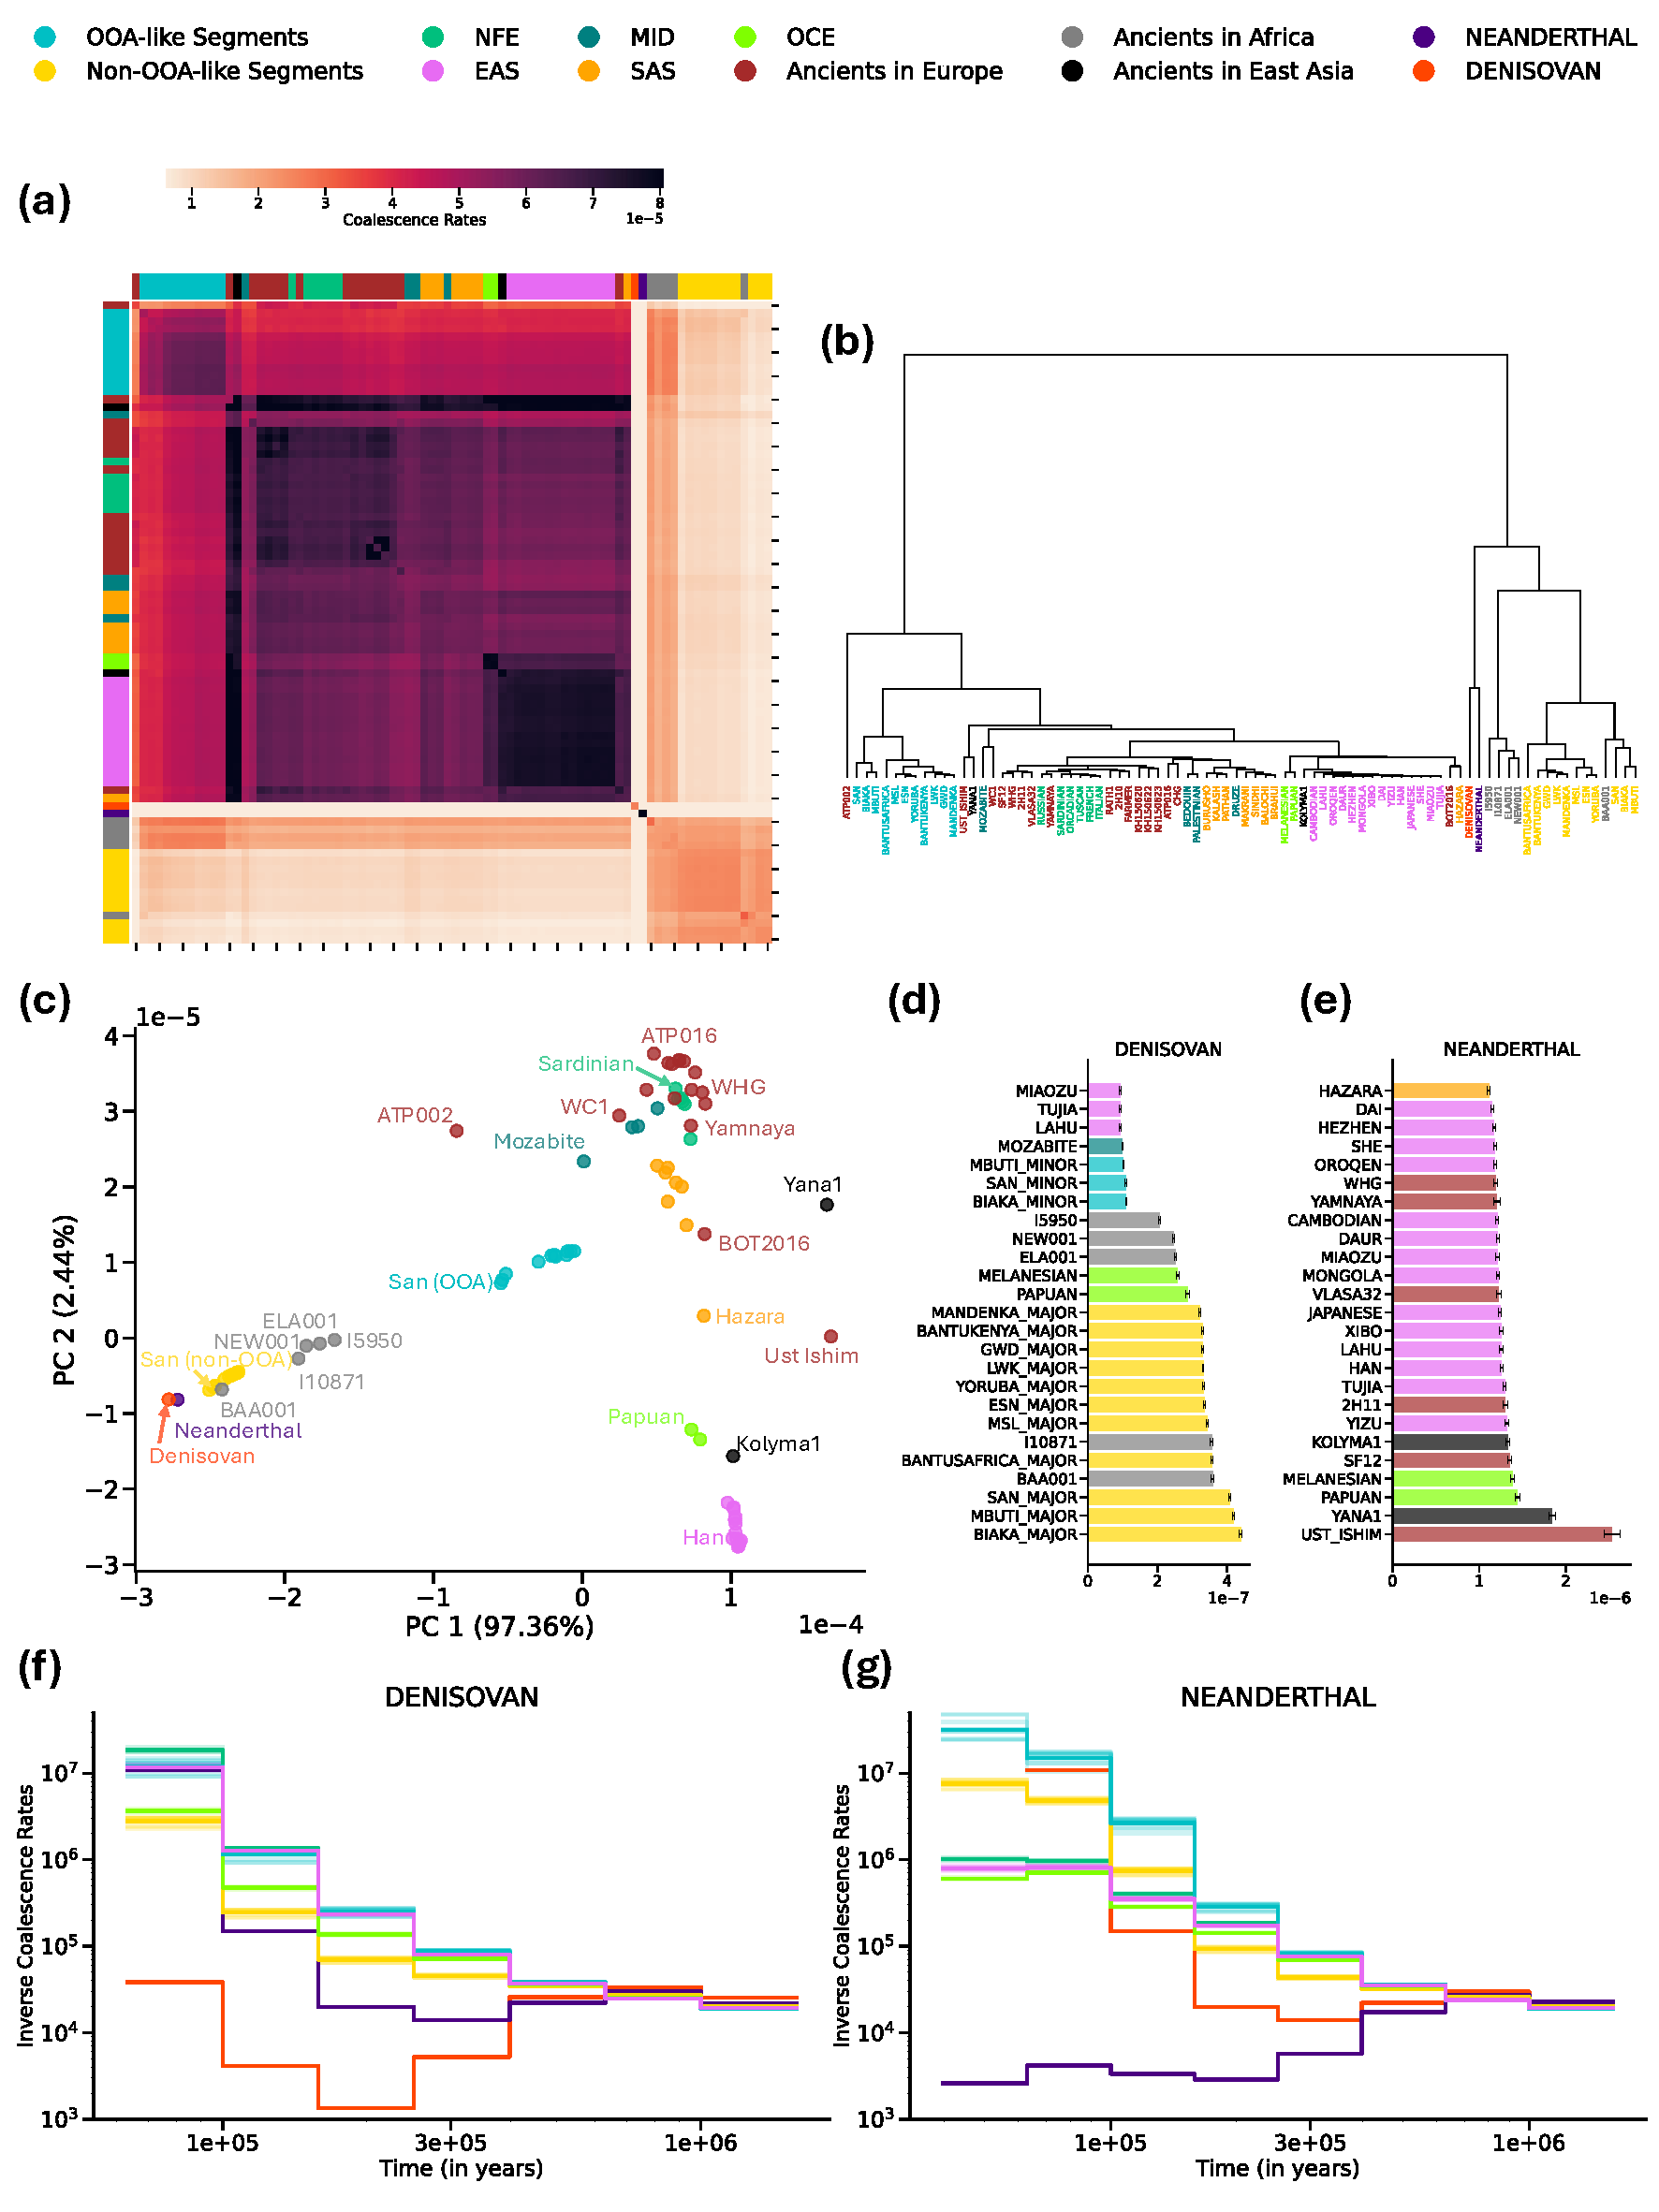
\includegraphics[width=\linewidth]{figures/gb_deepadmix/gb_real_deep_12.pdf}
    \captionsetup{width=\textwidth+3cm}
    \caption{
    \footnotesize
    \textbf{Coalescence rates with modern and ancient samples.} (a) Matrix of pairwise coalescence rates for all modern and ancient groups in the epoch spanning $64{,}000$–$100{,}000$ years. (b) Dendrogram corresponding to the UPGMA hierarchical clustering of the pairwise coalescence rate matrix in (a). (c) PCA visualization of coalescence rates for the epoch spanning $64{,}000$–$100{,}000$ years, with PC1 and PC2 representing the eigenvectors capturing the greatest variance among modern samples. (d-e) Top $25$ groups based on coalescence rates with (d) Denisovan, and (e) Neanderthals during the epoch spanning $64{,}000$–$100{,}000$ years. (f-g) Inverse coalescence rates (ICR) of (f) Denisovan and (g) Neanderthals with other modern human groups from $64{,}000$-$1.6$million years. Darker lines represent population-averaged ICRs.  Row and column colors in (a), dendrogram leaves in (b), dots and bars in (c-e), and lines in (f-g) are colored according to the common legend. NFE = non-Finnish Europeans, EAS = East Asians, MID = Middle Easterners and North Africans, SAS = South Asians, OCE = Oceanians. The numbers in brackets in (c) indicate the proportion of variance explained by each principal component. The error bars in (d-e) represent 95\% confidence intervals calculated using $100$ bootstraps. Results derived from HGDP+$1{,}000$GP+aDNA+archaic genealogies.
    }
\label{fig:gb-deepadmix-source}
\end{figure}

We analyzed coalescence rates in relation to archaic human groups, including three Neanderthal and one Denisovan sample. These samples clustered with the non-OOA-like component (see Figure \ref{fig:gb-deepadmix-source}b). To confirm this observation, we examined coalescence rates across different time epochs and found that both Denisovan and Neanderthal samples consistently exhibited closer relationships to the non-OOA-like component until approximately one million years ago, when all human lineages converge. The coalescence rate patterns suggest ancient migration or admixture events involving these four human groups (see Figure \ref{fig:gb-deepadmix-source}d-g). Furthermore, inverse coalescence rates between Out-of-Africa-like (OOA-like) and non-OOA-like components reveal a deep ancestral split, with the two rates converging at least $300{,}000$ years ago (see Figure \ref{fig:gb_real_deep_coal_ooa}). This predates the divergence of the Eurasian population from the OOA-like component and occurs after the split of Neanderthals and Denisovans from the modern human lineage, although there may be considerable uncertainty in the exact split time.

\begin{figure}
    \centering
    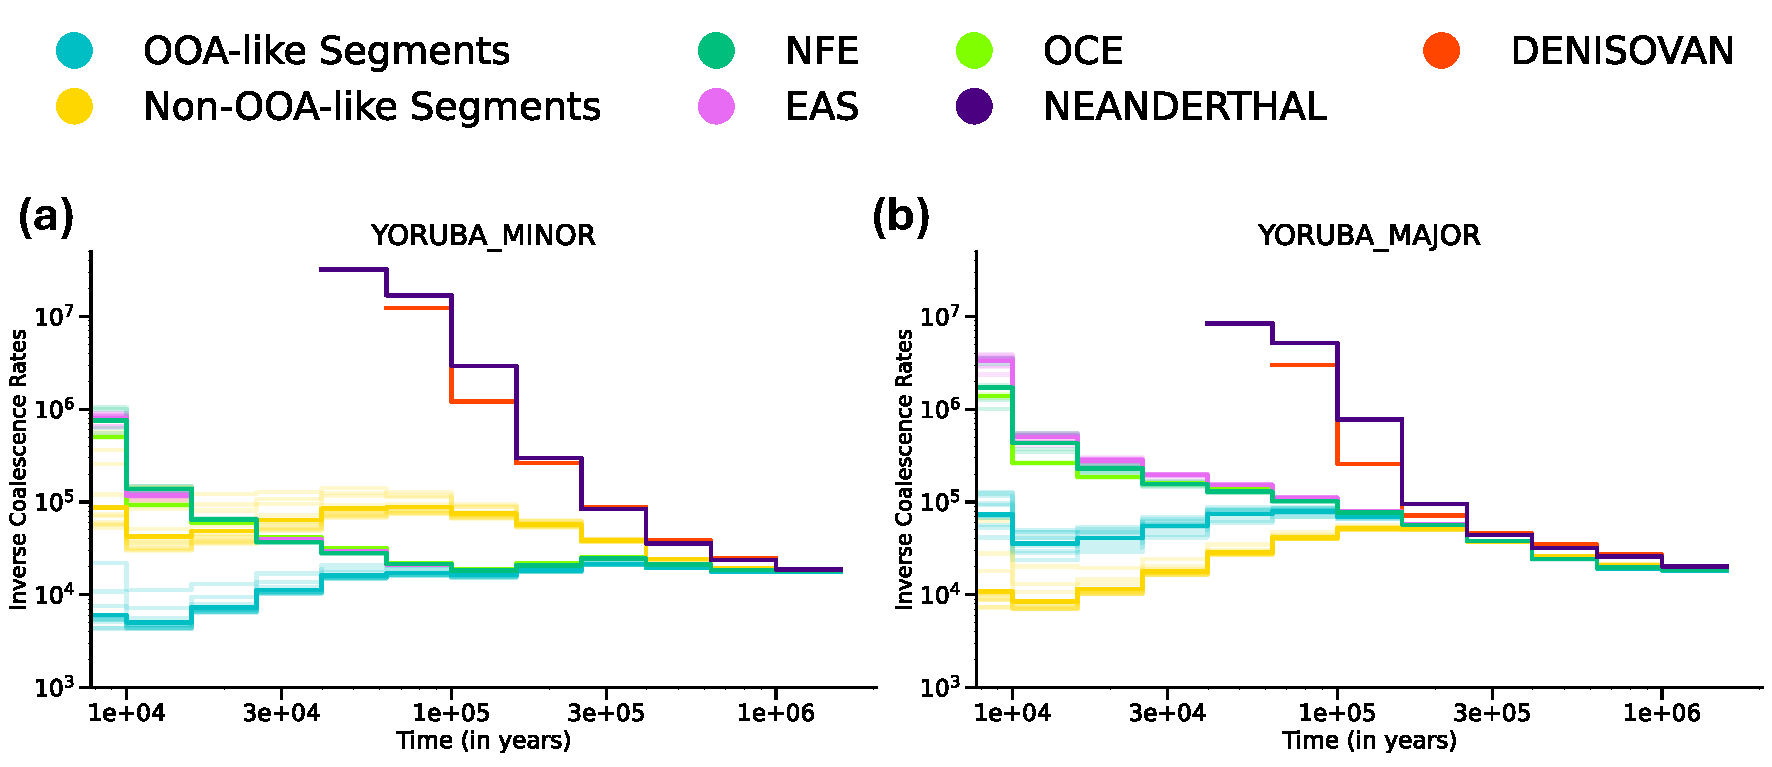
\includegraphics[width=\textwidth]{figures/gb_deepadmix/gb_real_deep_source_coal_rates.pdf}
    \caption{
    \textbf{Inverse coalescence rates (ICRs) of OOA-like and Non-OOA-like component in Yoruba.} ICRs of OOA-like (YOROBA\_MINOR) and Non-OOA-like (YORUBA\_MAJOR) components in Yoruba with other modern human and archaic groups from $64{,}000$-$1.6$million years ago. Darker lines represent population-averaged ICRs and fainter lines represent within population ICRs. NFE = non-Finnish Europeans, EAS = East Asians, MID = Middle Easterners and North Africans, SAS = South Asians, OCE = Oceanians.}
\label{fig:gb_real_deep_coal_ooa}
\end{figure}



\clearpage

\subsection{Impact of the admixture event on polygenic score portability in Africa}

Polygenic scores (PGS) evaluate an individual's genetic predisposition to specific diseases or traits, providing valuable insights into personalized health risks. A PGS is derived from large-scale genome-wide association studies (GWAS), which identify associations between genetic variants and traits of interest. These associations are then used to calculate the risk for a disease or the predisposition to a complex trait. PGSs have been transformative in personalized medicine and is increasingly being applied in clinical settings \cite{torkamani2018personal,lewis2020polygenic}. However, despite their success, a major limitation of PGS is their reduced accuracy and predictive power across diverse ancestral backgrounds \cite{martin2019clinical, ding2023polygenic}. The majority of polygenic scores (PGS) are derived from genome-wide association studies (GWAS) conducted predominantly on populations of European ancestry, resulting in limited ``portability'' when applied to non-European populations. One key reason for this lack of portability is the difference in Linkage Disequilibrium (LD) patterns and allele frequencies between ancestrally diverged groups. Since PGS are typically based on common variants that serve as proxies for underlying causal mutations, differences in LD between the causal and tag variants or shifts in the frequency of these variants can introduce bias. This bias is most pronounced in individuals who are genetically distant from the GWAS reference population \cite{ding2023polygenic}. We aim to investigate the differences in PGS portability for African individuals in the UK Biobank. Specifically, in the context of the deep admixture event, we aim to determine whether the two ancestral components in Africa exhibit differences in PGS portability across a broad range of phenotypes. Furthermore, given our hypothesis that the OOA-like population significantly contributed to the ancestry of European individuals, we anticipate this analysis will reveal higher PGS portability for segments derived from the OOA-like population compared to those derived from the non-OOA-like population.

We used posterior mean effect estimates from the recent GWAS method Quickdraws to calculate polygenic scores (PGS) for several quantitative traits in the UK Biobank, utilizing data from up to $405{,}000$ white British individuals for model fitting. Detailed information on Quickdraws and the PGS calculation methodology can be found in Chapter \ref{ch:4-qd-method} and Section \ref{sec:ch5-qd-pgs}. The traits analyzed included blood-related phenotypes, anthropometric measurements, and other quantitative traits (see Table \ref{tab:ukb_qt_traits} for a full list). We focused our analysis on $32$ phenotypes selected based on the predictive power of polygenic scores (PGS) in Europeans ($R^2 > 0.1$) and a high phenotyping rate in self-identified Africans (phenotyping rate $> 0.9$). Figure \ref{fig:gb_deepadmix_anchor}a illustrates the prediction $R^2$ achieved using the calculated PGS across various self-identified ancestry groups and phenotypes. For several phenotypes, we observed that the predictive power in African individuals dropped to approximately $20\%$ of the prediction $R^2$ observed in European populations.

% We perform our analysis on $6{,}159$ self-reported African individuals in the UK Biobank which have previously been shown to have African ancestry as their majority ancestry. Across all traits and $6{,}159$ African individuals, we observed a substantial reduction in PGS accuracy, with predictive power dropping to approximately 20\% of the accuracy observed in European populations (see Figure \ref{}a).

To examine differences in PGS portability across the two ancestries identified using GhostBuster -- namely, OOA-like and non-OOA-like -- we began by phasing the UK Biobank SNP array data using \texttt{SHAPEIT4} \cite{delaneau2019accurate}. We filtered the data to retain only $4{,}557$ African samples with less than 10\% recent European admixture, as inferred using \texttt{hapmix} \cite{price2009sensitive,hu2023leveraging}. The phased haplotypes were then lifted over to the hg38 genome build. To infer the ancestral components within these African samples, we utilized an optimized implementation of \texttt{Chromopainter} \cite{Lawson2012}, using African samples from the HGDP and $1{,}000$ Genomes Project as the reference panel. Chromosome painting was performed with parameters optimized through initial fitting on a subset of the data: a mutation probability per SNP of $\theta = 0.0011$ and a recombination scaling factor $\rho = 368.43$. This process assigned each genomic site in the UK Biobank African samples a posterior probability of copying from individuals in the reference panel. For each site, we selected the top 20 reference individuals with the highest posterior probabilities and normalized these probabilities so their sum equaled one. Using local ancestry inference from GhostBuster and the HGDP+$1{,}000$GP reference panel, we then estimated local ancestry in the UK Biobank African samples by calculating a weighted average of local ancestry posteriors, with weights determined by the \texttt{Chromopainter} copying probabilities. Overall, we obtained an estimate of the local ancestry corresponding to the two ancestral components in $4{,}557$ phased African samples from the UK Biobank. 

To examine differences in the predictive ability of PGS across the two ancestral components, we decomposed the PGS of an African individual into OOA-like and non-OOA-like components, conditioned on the local ancestry of the sample, following the pipeline described in \cite{hu2023leveraging}. The decomposition begins by estimating the expected allele counts for each ancestry background as follows:
\begin{align}
    H^{c}_{i,j} &= H_{i,j} * P(L_{i,j} = c) \nonumber \\
    G^{c}_{i,j} &= H^{c}_{i_1,j} + H^{c}_{i_2,j}
\end{align}
where, $H_{i,j}$ represents the phased haplotype of sample $i$ (with $i_1$ and $i_2$ indexing the haplotypes of sample $i$) at variant position $j$, $L_{i,j}$ is the local ancestry of sample $i$ at position $j$, and $G^{c}_{i,j}$ is the expected allele count for ancestry background $c \in \{\text{OOA-like}, \text{non-OOA-like}\}$. As suggested in \cite{hu2023leveraging}, we mean-center these genotypes before calculating ancestry-specific PGS as follows:
\begin{center}
\resizebox{\textwidth}{!}{%
\begin{minipage}{\textwidth}
\begin{align}
\bar{G}_{ij}^{\text{OOA-like}} &= G_{ij}^{\text{OOA-like}} - 2f_j^{\text{OOA-like}} \left( P_{ij}^{\text{OOA-like, OOA-like}} + P_{ij}^{\text{OOA-like, non-OOA-like}} \right), \nonumber \\
\bar{G}_{ij}^{\text{non-OOA-like}} &= G_{ij}^{\text{non-OOA-like}} - 2f_j^{\text{non-OOA-like}} \left( P_{ij}^{\text{non-OOA-like, non-OOA-like}} + P_{ij}^{\text{OOA-like, non-OOA-like}} \right)
\end{align}
\end{minipage}
}
\end{center}
where, $\bar{G}_{ij}^{c}$ is the mean-centered genotype for ancestry background $c$. $P_{ij}^{c_1, c_2}$ denotes the local ancestry product across the two haplotypes, calculated as $P_{ij}^{c_1, c_2} = P(L_{i_1,j} = c_1) * P(L_{i_2,j} = c_2)$, where $i_1$ and $i_2$ represent the two haplotypes of an individual. The frequency $f^{\text{OOA-like}}$ is determined using an OLS regression of the observed genotype given the local ancestry:
\begin{align}
    G_{ij} = I_j + S_j \ast \left( 2P_{ij}^{\text{OOA-like, OOA-like}} + 2P_{ij}^{\text{OOA-like, non-OOA-like}} \right) + \varepsilon_i \nonumber \\
    f^{\text{OOA-like}} = S_j + \frac{I_j}{2} \quad \text{and} \quad f_j^{\text{non-OOA-like}} = \frac{I_j}{2}
\end{align}

Finally the ancestry specific PGS can be obtained by multiplying the posterior mean effect estimates and mean-centered genotypes as follows:
\begin{align}
    PGS_{\text{OOA-like}, i} &=  \sum_{j} \hat{\beta}_j \bar{G}_{ij}^{\text{OOA-like}} \\ \nonumber 
    PGS_{\text{non-OOA-like}, i} &= \sum_{j} \hat{\beta}_j \bar{G}_{ij}^{\text{non-OOA-like}}
\end{align}
where, $\hat{\beta}_j$ is the posterior mean effect or PGS beta for variant $j$. To estimate the role of ancestry specific PGS in predicting the phenotype we fit a linear regression of the form:
\begin{equation}
    Y_i = I + \beta_{\text{OOA-like}} PGS_{\text{OOA-like}, i} + \beta_{\text{non-OOA-like}} PGS_{\text{non-OOA-like}, i} + \alpha \text{Covariates}_i
\end{equation}
Here, $\beta_{\text{OOA-like}}$ and $\beta_{\text{non-OOA-like}}$ represent the predictive ability of the PGS based on the OOA-like and non-OOA-like ancestry components for phenotype $Y$. These coefficients were estimated using ordinary least squares (OLS) regression, and their confidence intervals were derived from $1{,}000$ bootstrap resamples of the individuals. Finally, the effect estimates were normalized by the corresponding effect estimates obtained from non-British self-identified European individuals, providing a measure of predictive ability relative to European samples.

We evaluated the predictive ability of PGS based on the two ancestry components across $32$ quantitative phenotypes in $4{,}557$ African samples. The predictive ability of the OOA-like component, $\beta_{\text{OOA-like}}$, was higher than that of the non-OOA-like component, $\beta_{\text{non-OOA-like}}$, in $28$ out of $32$ traits (paired t-test $p = 5.3 \times 10^{-6}$, see Figure \ref{fig:gb_deepadmix_anchor}b). An inverse-variance meta-analysis across 32 phenotypes showed a 35\% higher effect size (\(\beta_{\text{OOA-like, meta}} = 0.81\), \(\beta_{\text{Non-OOA-like, meta}} = 0.6\)) and approximately 82\% greater predictive power as measured by \(R^2\)), which scales with the square of the effect size. Among the phenotypes analyzed, total bilirubin levels exhibited predictive power greater than $1$ in both components, as its predictive ability in Africans was comparable to that in Europeans (see Figure \ref{fig:gb_deepadmix_anchor}a). Certain phenotypes, such as gamma-glutamyl transferase (GGT) and Apolipoprotein B, showed substantial differences in predictive ability between the two components. GGT demonstrated significantly higher predictive power in the OOA-like component ($\beta_{\text{OOA-like}} = 0.98$, $\beta_{\text{non-OOA-like}} = 0.06$) but low prediction $R^2$ overall, whereas Apolipoprotein B showed greater predictive power in the non-OOA-like component ($\beta_{\text{OOA-like}} = 0.34$, $\beta_{\text{non-OOA-like}} = 0.92$). This discrepancy is likely attributable to the oligogenic nature of these traits, with only a small number of genomic regions controlling the phenotype \cite{vuckovic2020polygenic}. Manhattan plots for these traits are presented in Figure \ref{fig:gb_anchor_man}.

\begin{figure}[h!]
    \centering
    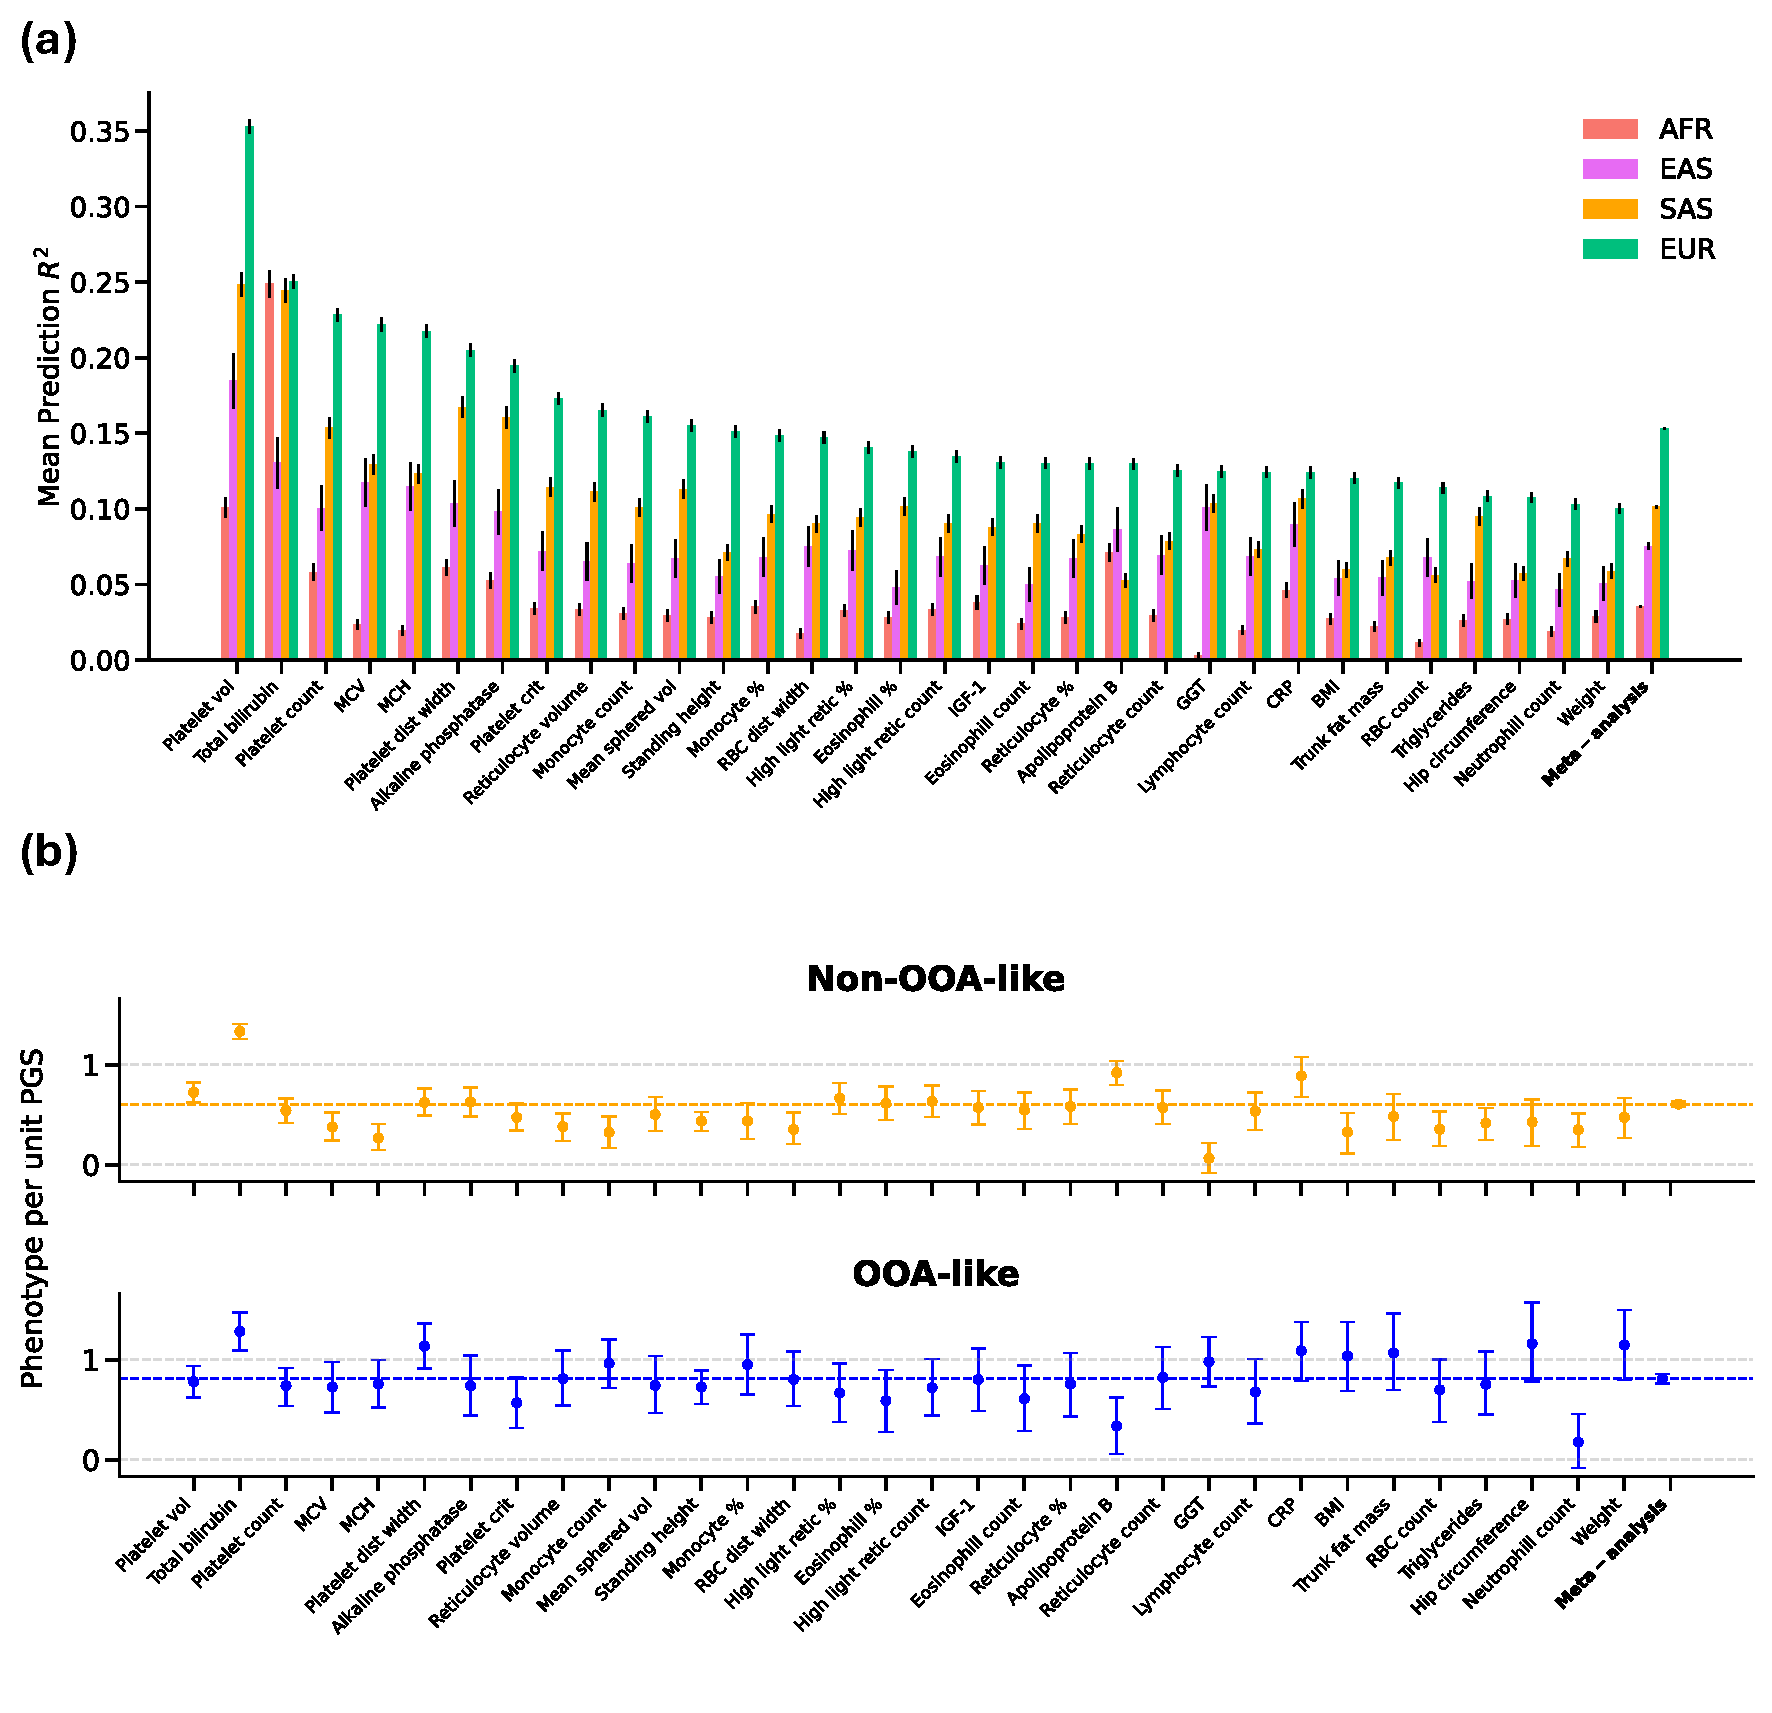
\includegraphics[width=\linewidth]{figures/gb_deepadmix/gb_real_deep_5.pdf}
    \captionsetup{width=\textwidth+3cm}
    \caption{
    \footnotesize
    \textbf{Differences in PGS predictive power across populations and deep admixture components.} (a) PGS prediction $R^2$ across $32$ quantitative phenotypes and four population groups: self-identified non-British Europeans (EUR), South Asians (SAS), East Asians (EAS), and Africans (AFR). Error bars represent the 95\% confidence intervals for the prediction $R^2$. (b) Normalized predictive ability of the PGS based on the OOA-like and non-OOA-like ancestry components across the same $32$ quantitative phenotypes. Error bars represent the 95\% confidence intervals calculated using $1{,}000$ bootstrap replicates. Traits are sorted based on their prediction $R^2$ in Europeans. PGS was calculated using posterior mean effect estimates obtained during Quickdraws' model fitting step. A meta-analysis using inverse variance-weighted average across traits is presented in (a) and (b).
    }
    \label{fig:gb_deepadmix_anchor}
\end{figure}

\clearpage

\section{Discussion}
\label{sec:ch3-discussion}

% Paragraph 1 is Summary/interpretation of major findings + their importance
% Paragraph 2 (optional) is Discussion of other methods
% Paragraph 3 is Implications for downstream analyses
% Paragraph 4 is Limitations and future work

% Genealogies offer a more direct understanding of human past, offering a more interpretable and powerful approach to understand admixture and migration history. 
% In this work we present, GhostBuster a mixture model which leverages the inferred genealogies to understand and infer admixture events in the past.
% GhostBuster offers state-of-the-art power to detect recent and ancient admixture events in simulations and established real-data examples.
% Analyzing recent and ancient events in Africa, we find evidence for widespread back to Africa migration, which has resulted up to 20\% ancestry in some sub-saharan African samples. 
% We validate and characterize this admixture event across different African populations, and find the migration bought with it Neanderthal ancestry explaining the non-zero Neanderthal ancestry in Africans, and elevated TCC to TTC mutation rates.
% We hypothesize the groups contributing this Eurasian ancestry might be associated with present day north Africans, and Anatolian farmers from Europe. 
% We also find evidence for a ancient admixture event between groups with differential coalescence rates with modern-day Eurasians.
% This deep admixture model supports the presence of two ancient populations, where one population resembles the out of Africa population, which migrated out of African and eventually gave rise to Eurasians. 
% We find difference in PGS portability among African samples dependent on this ancestry decomposition. 


Genealogies provide a powerful and interpretable framework for understanding human history. In this work, we introduce GhostBuster, a mixture model that leverages inferred genealogies to detect and analyze historical admixture events. GhostBuster identifies patterns in the coalescence history of target individuals, clustering these patterns to detect ancestry differences across the genome. In simulations involving both modern and ancient gene flow, GhostBuster demonstrated high power for detecting admixture events and provided more accurate local ancestry inference than traditional HMM-based methods \cite{skov2018detecting}. In real data examples, including admixture events within the past $2{,}000$ years, GhostBuster’s results aligned closely with previous haplotype-based methods \cite{salter2019fine}, underscoring its robust capability to detect recent gene flow events.

We applied GhostBuster to investigate the population history of Africa by analyzing joint genealogies inferred from publicly available modern and ancient populations. Our analysis began by focusing on admixture history in the context of back-to-Africa migration \cite{pickrell2012genetic, llorente2015ancient, chen2020identifying}. Using GhostBuster, we uncovered widespread back-to-Africa migration from Eurasia, contributing an average of approximately $2.5\%$ and up to $10\%$ Eurasian ancestry across all present-day African populations analyzed. We identified previously unrecognized ancient back-migration events in several populations, particularly in West and Central Africa, while corroborating previously documented back-migration events in East and South Africa \cite{pickrell2014ancient, llorente2015ancient}. We estimated the timing of these admixture events ranged from the past millennium to approximately $10{,}000$ years ago, coinciding with the end of the last Ice Age and aligning with the Green Sahara period \cite{tierney2017rainfall, larrasoana2013dynamics}, when the Sahara was likely more navigable. Characterizing and validating the admixture event, we also found that this back-migration event alone provides a plausible explanation for the presence of small amounts of Neanderthal ancestry in African genomes. Furthermore, the Eurasian segments in Africans exhibited distinct mutational profiles, including elevated TCC to TTC mutations, and showed genetic proximity to populations in modern-day North Africa, the Middle East, and Anatolian farmer-related groups. These findings suggest a connection between this migration and the spread of farming practices from Europe into Africa.

%Overall, GhostBuster’s ancestry partitioning, further validated by independent validations like Neanderthal ancestry overlap and enriched TCC to TTC mutation rates, provides a clearer and more comprehensive view of the extent and impact of this back-to-Africa migration. 

In addition to the back to Africa migration, we applied GhostBuster to examine deeper population history in Africa, focusing on events from $10{,}000$ years ago and earlier. Previous studies have proposed various hypotheses including presence of ghost populations \cite{skoglund2017reconstructing,durvasula2020recovering}, weak structured stem \cite{ragsdale2023weakly}, and ancient migrations \cite{lipson2020ancient} to explain the complex population structure in sub-Saharan Africa. Using GhostBuster, we identified two distinct ancestral components in the African genome, differentiated by their coalescence rates with Eurasians. We hypothesize that these components reflect an ancient admixture event occurring around or after the out-of-Africa migration, involving two ancestral populations. One of these populations likely represents a group closely related to the out-of-Africa population. We observed significant differences in population sizes and historical hotspot activity between these ancient groups, as evidenced by variations in weak to strong mutation rates across the genome and at specific recombination hotspots. Additionally, we identified differential affinities of the two components with archaic human groups, including Neanderthals and Denisovans, and found evidence of a deep population split between the two components, occurring at least $300{,}000$ years ago. Finally, our analysis of African individuals in the UK Biobank revealed substantial differences in polygenic score (PGS) portability between these two ancestral components when European GWAS data were used for PGS construction.

%This finding emphasizes the importance of ancestry decomposition in PGS analyses, highlighting how deep population structure can shape genetic predictions within African populations.
Overall, GhostBuster proved effective in characterizing previously known admixtures while uncovering new insights into more ancient admixture events in Africa. We believe GhostBuster can be leveraged to investigate a wide range of admixture events, both recent and ancient, offering valuable insights with numerous downstream applications. For instance, admixture inference is crucial for understanding the evolutionary history of species, shedding light on the complex dynamics of migration, adaptation, and gene flow that have shaped modern populations. By inferring local ancestry along the genome, GhostBuster enables the identification of regions involved in adaptive admixture, where genes from one population may confer selective advantages in another. Furthermore, GhostBuster’s ability to detect and analyze fine-scale admixture has significant implications for medical genetics, helping researchers uncover the genetic basis of phenotypic variation across populations, including differences in disease susceptibility and other health-related traits.


\subsection{Limitations and future work}

We identify several current limitations and areas for future improvement. First, GhostBuster uses genome-wide genealogies, which generally requires high-coverage sequencing data to accurately infer genetic relationships between samples. However, many ancient DNA samples are sequenced at low coverage, limiting their integration into current genealogy inference methods. Addressing this challenge through scalable ``threading'' techniques to incorporate low-coverage ancient DNA into genealogies, or through imputation methods \cite{rubinacci2021efficient, sousa2023imputation}, could significantly expand the number of ancient samples available for analysis. This would greatly improve GhostBuster’s capacity to provide a comprehensive view of population history, particularly in cases where admixture signals are subtle and may not be apparent from limited high-coverage ancient DNA or modern samples -- such as in the complex 3-way admixture observed in Europe (see Section \ref{sec:ch2-gb-real-eur}). 

% Second, genomic biases (such as those introduced by background selection) or errors in genealogy inference can occasionally produce false admixture signals. As demonstrated in our simulations (see Section \ref{sec:ch2-gb-sim}), biases during genealogy inference are typically mitigated by evaluating the held-out log-likelihood, assessing confidence in local ancestry inference, and analyzing coancestry curve dating. In contrast, biases along the genome due to background selection or other genomic factors can be identified through admixture dating and examining correlations with metrics of background statistics. Advancements in genealogy inference methods to reduce biases and increase reconstruction accuracy would further strengthen our model's reliability, making this an important direction for future research. 

Second, biases in genealogy inference can occasionally produce false admixture signals, as shown in our simulations (see Section \ref{sec:ch2-gb-sim}). Typically, these biases are mitigated by evaluating the held-out log-likelihood, assessing confidence in local ancestry inference, and analyzing coancestry curve dating. Advancements in genealogy inference methods to reduce biases and increase reconstruction accuracy would further strengthen our model’s reliability, making this an important direction for future research.


Third, GhostBuster is computationally slower than some other ancestry inference software that rely on low-dimensional summary statistics. While these alternatives often lack the statistical power to detect subtle admixture signals, there are promising strategies to improve GhostBuster’s computational efficiency. For instance, using PCA on the coalescence count matrix generated by GhostBuster can provide a fast, approximate inference of admixture. Additionally, implementing GhostBuster in a low-level programming language or leveraging modern computing architectures like GPUs could significantly improve its speed, making it more feasible for large-scale analyses. We propose these improvements as directions for future work. Finally, expanding the use of GhostBuster to study the evolutionary history of other species would also be highly beneficial. In the next section, we demonstrate its effectiveness in uncovering an admixture event in American wolves. We believe that GhostBuster could similarly aid in understanding the population dynamics and admixture history of several other species, paving the way for broader applications in evolutionary biology. 

% - Low coverage ancients and threading
% - sampling from the genealogies to increase robustness to errors
% - Depends on labelling of reference populations 
% - Choosing number of components needs more work

\subsection{Understanding admixtures in non human organisms}

To demonstrate the ability of GhostBuster to detect admixture beyond humans, we applied it to understand the admixture history of North American wolves. We analyzed five American Great Lakes wolves alongside one Coyote and 29 European grey wolf genomes. Previous research has shown that Great Lakes wolves have undergone admixture with Coyotes over the last few thousand years \cite{lehman1991introgression,bozarth2011coyote,vonholdt2016whole}. We used the Relate trees and dataset from \cite{bergstrom2022grey}, along with a canid recombination map from \cite{auton2013genetic}. GhostBuster was run with two components, considering coalescence events over a wide time interval ranging from $100$ years to one million years. Our analysis revealed that the major component, contributing approximately around three quarters, was closer to grey wolves, while the minor component was closer to the coyote sample in the dataset. Using coancestry curve fitting, we identified the two-date admixture model as the best fit for the observed coancestry curves. The inferred admixture dates were $186.7$ generations ($560.1$ years) and $1777.7$ generations ($5{,}333.1$ years), with $79$\% of the observed admixture attributed to the older admixture date. See Figure \ref{fig:gb_real_wolves} for further details.

\begin{figure}[h!]
    \centering
    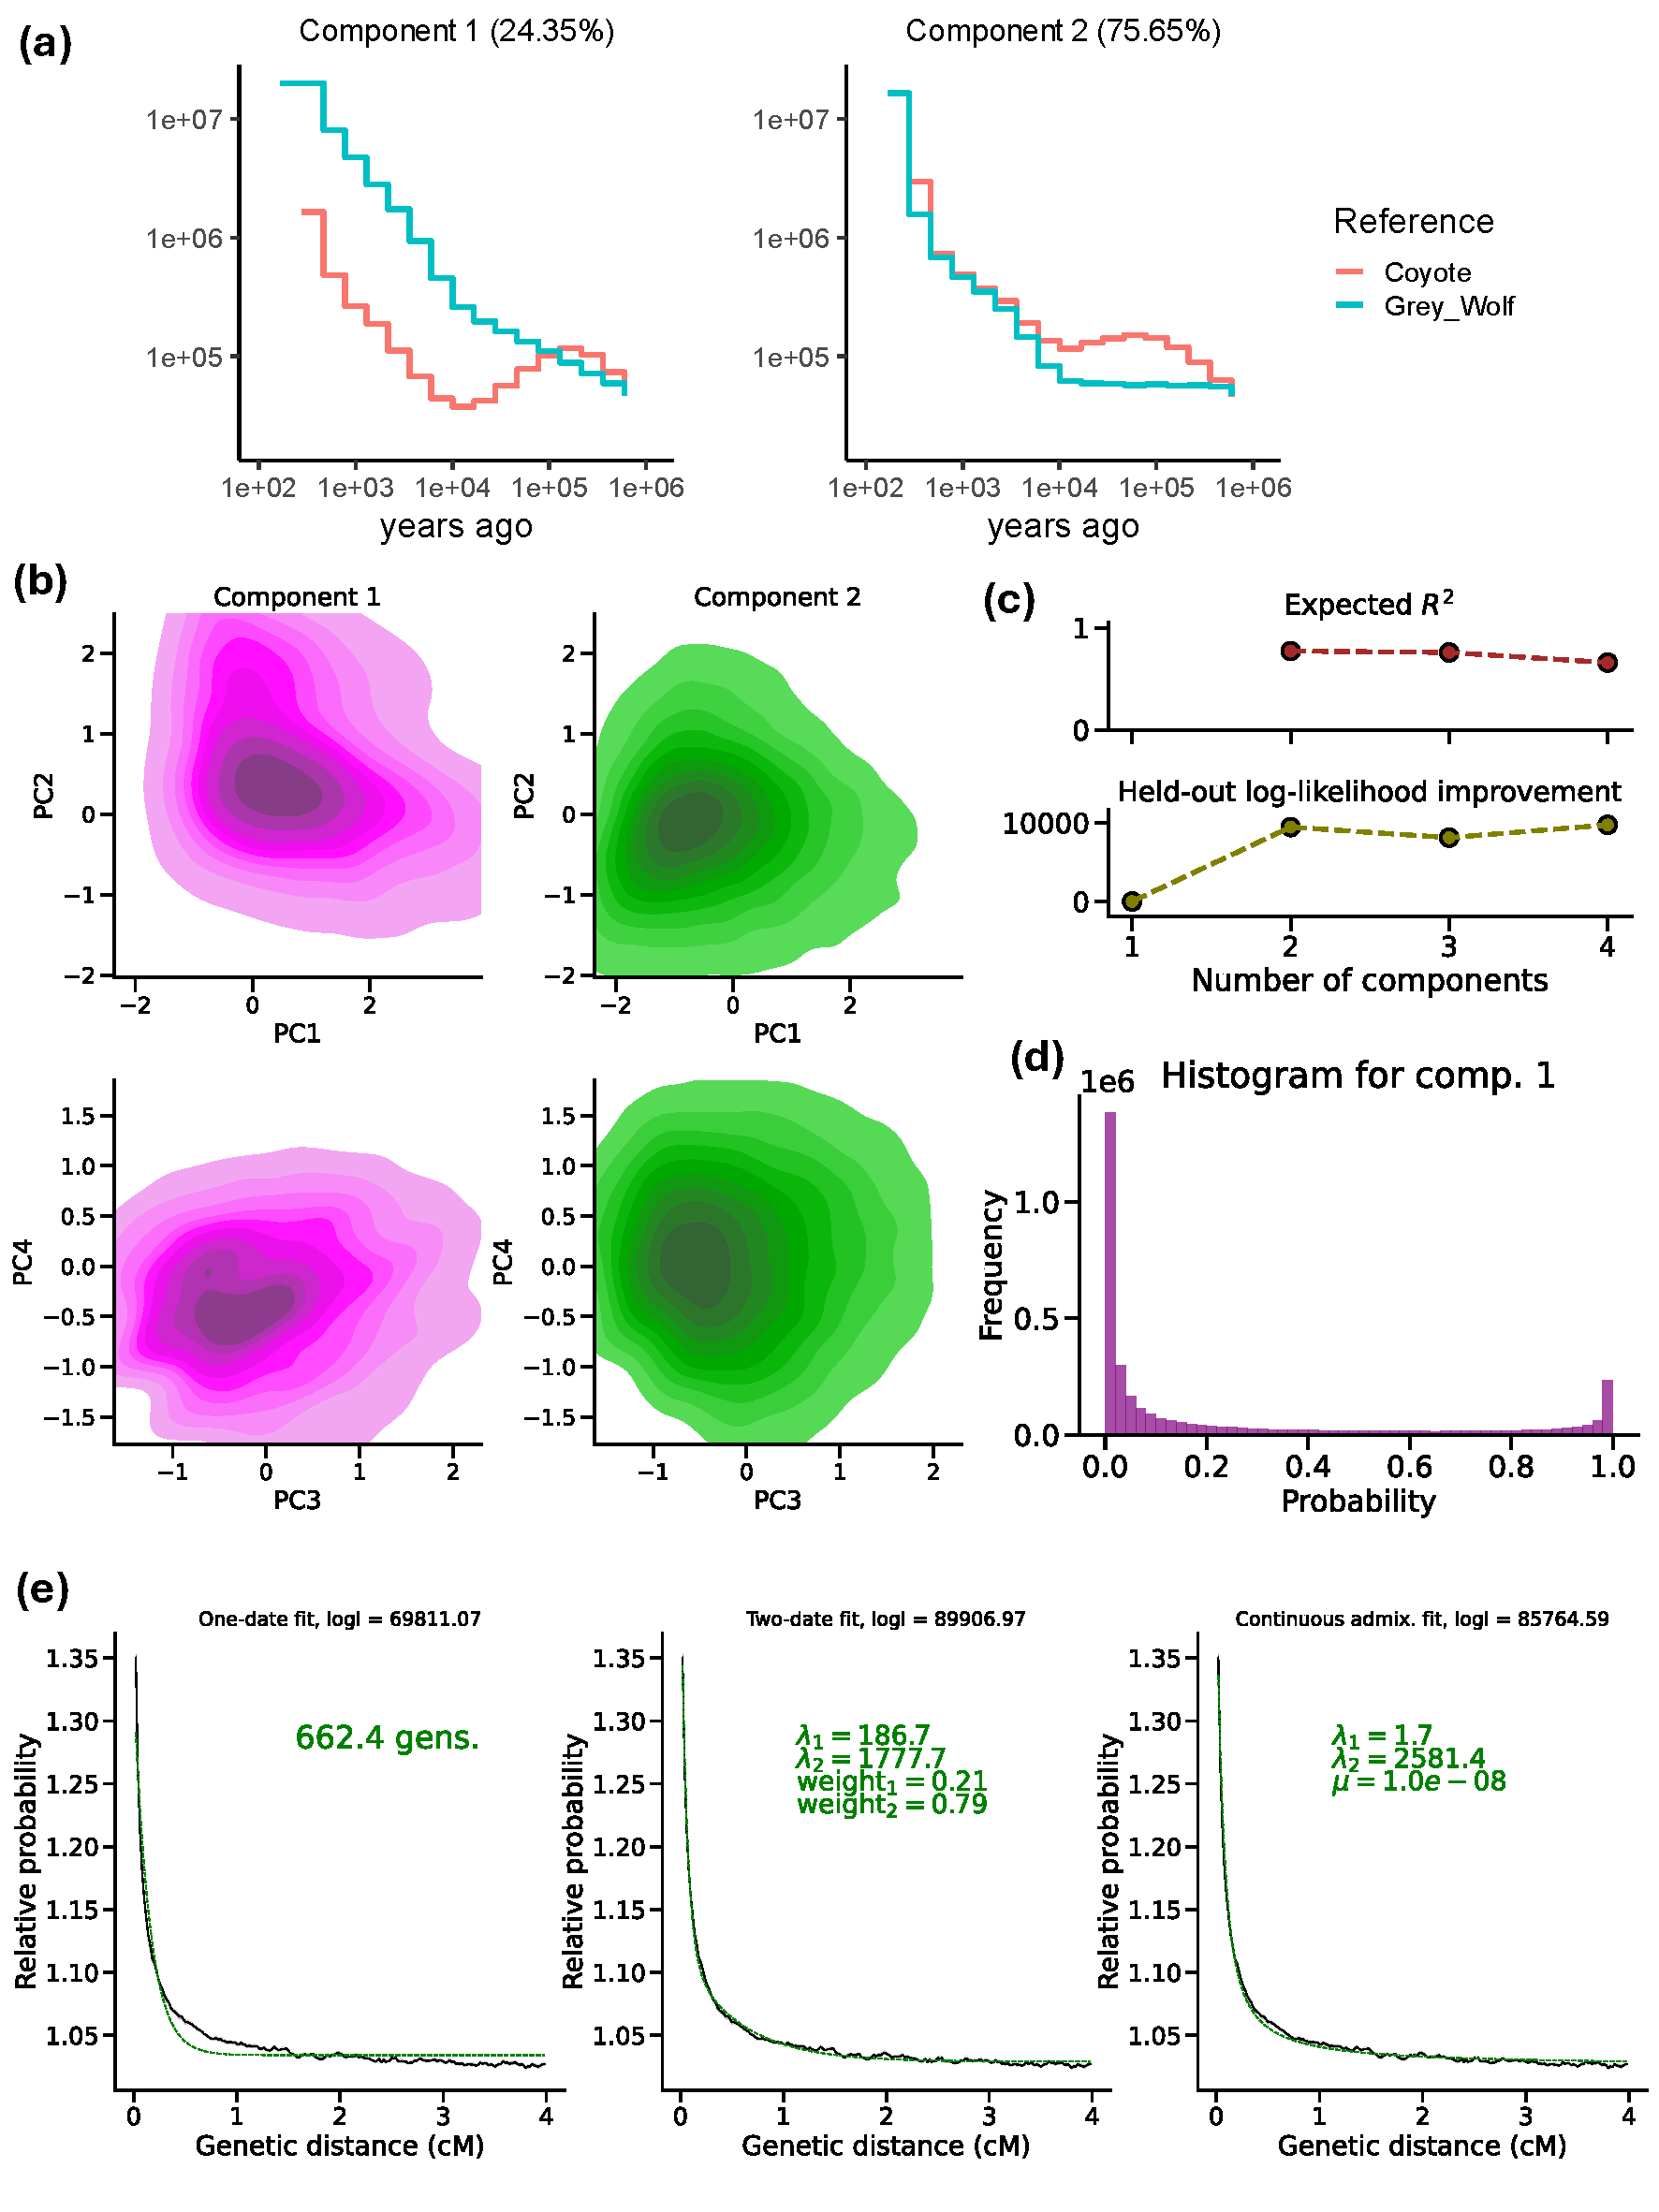
\includegraphics[width=\linewidth]{figures/gb_sims/gb_real_wolves.pdf}
    \captionsetup{width=\textwidth+3cm}
    \caption{
    \footnotesize
    \textbf{Decomposing American wolves with grey wolves and coyote as reference.} (a) Inferred inverse coalescence rates and proportions: each line represents inverse coalescence rate profiles with a reference population. (b) PCA visualization of the coalescence count and opportunity matrix derived from the genealogies plotted separately for each component. (c) Expected coefficient of determination and held-out log-likelihood improvement with varying number of components. (d)  Histogram of the inferred local ancestry posteriors. (e) Coancestry curves and model fit for one-date, two-date, and continuous migration scenarios (admixture dates in generations). The figure title includes `logl', which refers to the log-likelihood of the fit (higher values indicate a better fit). The PCA visualization in (b) is based on a KDE plot with a threshold of 0.05, and binary local ancestry estimates are obtained by thresholding the inferred posteriors at 0.5.
    }
    \label{fig:gb_real_wolves}
\end{figure}
\chapter{\label{ch:4-qd-method}A scalable variational inference approach for increased mixed-model association power}

\minitoc

\section{Chapter overview}
In this chapter, we introduce a novel method called Quickdraws, which we developed to perform scalable and statistically powerful genome-wide association studies. Quickdraws leverages advancements in machine learning and the processing power of modern computing architectures, such as graphical processing units (GPUs), to conduct genome-wide association studies on a large scale. We begin by presenting the theoretical framework for Quickdraws in section \ref{sec:ch4-theory}, which incorporates modern variational inference techniques, including stochastic variational inference. After establishing the theoretical foundation, we will delve into the algorithm's details in section \ref{sec:ch4-method}, covering several steps such as heritability estimation, Bayesian regression, and the estimation and calibration of test statistics. Finally we summarize the key steps in the algorithm in section \ref{sec:ch4-summary}.

\begin{figure}[h!]
    \centering
    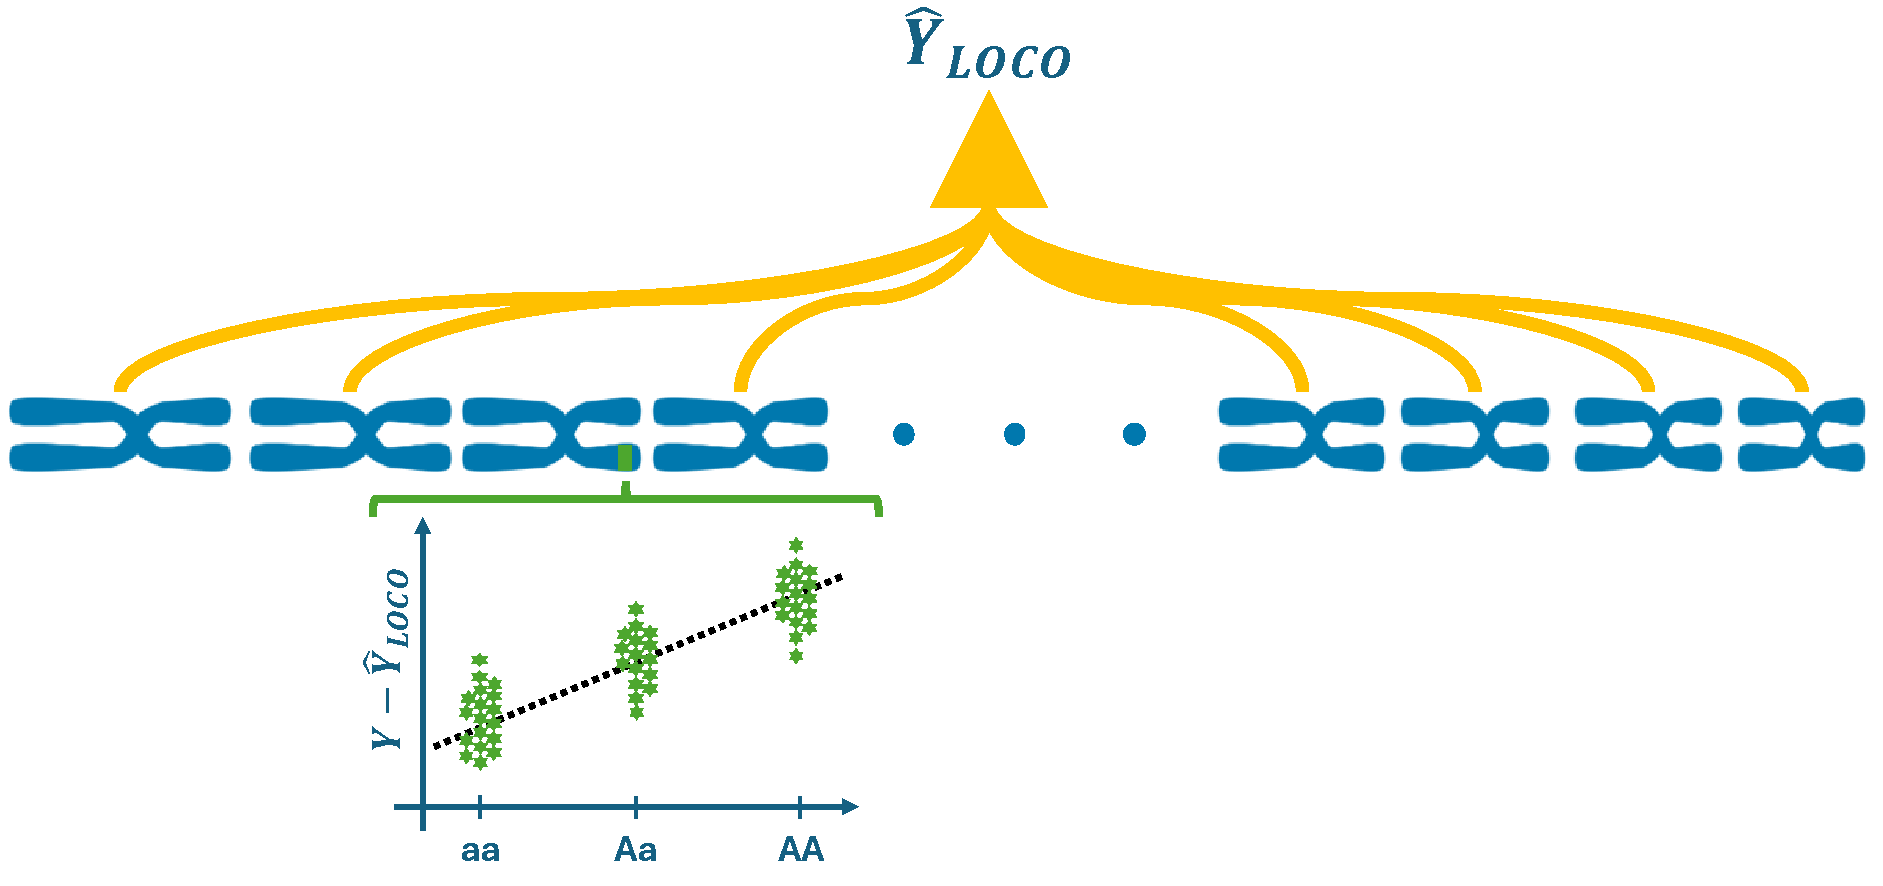
\includegraphics[width=\textwidth]{figures/thesis_qd_simplified_overview.pdf}
    \caption{\textbf{A simplified overview of Quickdraws.} Quickdraws is a scalable mixed model designed for genome-wide association studies (GWAS). It improves the power of association testing through a two-step process. First, it estimates the genomic prediction for a trait by excluding the testing chromosome, employing a leave-one-chromosome-out method. The prediction models sparsity of effects and is optimized using advanced variational inference techniques ensuring scalability for large sample sizes. Second, the model leverages this genomic prediction to improve the signal-to-noise ratio for finding association between a trait and a variant.}
    \label{fig:qd-simplified-overview}
\end{figure}

\section{Theoretical framework for our method}
\label{sec:ch4-theory}
\subsection{Bayesian inference}
Bayesian inference is a popular statistical inference approach that takes into account prior beliefs about the model along with evidence obtained from the data.
%
We introduce some basic terminology related to Bayesian inference, which we utilize in the following sections to describe our inference approach.
%
We refer the reader to \cite{blei2017variational,bishop2006pattern} for a more in-depth review on Bayesian inference and variational Bayes approaches.
%
We use the following notation and terminology:
%
\begin{itemize}
    \item $X = (x_1, x_2, ..., x_n)$ is a set of $n$ observed data-points 
    \item $\theta$ parameterizes the probability distribution of the data-points, $x \sim P(x \mid \theta)$.
    \item The \textbf{prior} distribution, $P(\theta)$, is the distribution of the parameters before any data is observed.
    \item The \textbf{data likelihood} or likelihood, $P(X \mid \theta)$, is the distribution of the data conditioned on model parameters.
    \item The \textbf{evidence} or marginal likelihood is the distribution of the observed data marginalized over parameters,
    \begin{equation}
        P(X) = \int P(X \mid \theta) P(\theta) d \theta \nonumber.
    \end{equation} 
    
    \item The \textbf{posterior}, $P(\theta \mid X)$, is the distribution of the parameters after taking into account the observed data,
    \begin{equation}
        P(\theta \mid X) = \frac{P(X \mid \theta) P(\theta)}{P(X)} = \frac{P(X \mid \theta) P(\theta)}{\int P(X \mid \theta) P(\theta) d \theta} \nonumber.
    \end{equation}
    
\end{itemize}
%

%
In the context of Bayesian inference, we are most interested in deriving the posterior distribution given prior beliefs on the parameters.
%
Unless the likelihood and prior are conjugate, however, we generally cannot derive a closed-form solution for the posterior.
%
Thus, in more general and usually more complex scenarios, Bayesian Inference heavily relies on sampling approaches, such as MCMC, or approximate methods, such as variational Bayes, to infer the posterior.
\subsection{Variational inference}
Variational inference is a popular approximate inference technique often used to infer posterior estimates for models that do not allow for a closed-form solution for their posterior.
%
In variational inference, posterior inference is formulated as an optimization problem.
%
As the exact posterior probability is often intractable, we assume an approximate posterior family that is easy to evaluate.
%
We then optimize the parameters of this posterior family so that the Kullback–Leibler (KL) divergence between the approximate and true posteriors is sufficiently small:
\begin{equation}
    KL\left(q_{\omega} (\theta) \| P(\theta \mid X) \right) = \int q_{\omega} (\theta) \log \left( \frac{q_{\omega} (\theta)}{P(\theta \mid X)} \right) d \theta \label{kl},
\end{equation}
where $P(\theta \mid X)$ is the true posterior and $q_{\omega} (\theta)$ is the approximate posterior, parameterized by $\omega$ (also known as variational parameters).
%
Variational inference aims to minimize the KL divergence in Equation \ref{kl}, to obtain optimal variational parameters $\omega^{*}$: 
\begin{equation}
    \omega^{*} = \underset{\omega}{\mathrm{argmin}}KL(q_{\omega}(\theta)||P(\theta|\textbf{X})).
    \label{opti}
\end{equation}

\subsection{Evidence lower bound and mean-field variational inference}
\label{sec:ch4-theory-mfvi}
Note that Equation \ref{opti} poses an optimization problem that requires the calculation of KL divergence between approximate posterior and the true posterior.
%
However, this objective cannot be computed because it requires information about the posterior, which is not available in closed form.
%
We thus use the Bayes rule to simplify the above equation,
%

\begin{align}
    KL(q_{\omega}(\theta)||P(\theta|\textbf{X})) &= \mathbb{E}[log(q_{\omega}(\theta))] -\mathbb{E}[log(P(\theta|\textbf{X})] \nonumber \\
&= \mathbb{E}[log(q_{\omega}(\theta))] -\mathbb{E}[log(P(\theta,\textbf{X})] + log(P(\textbf{X})) \nonumber \\
& = KL(q_{\omega}(\theta)||P(\theta)) -  \mathbb{E}[log(P( \textbf{X}|\theta)] + log(P(\textbf{X})) \geq 0
\end{align} 
\begin{equation}
    \implies log(P(\textbf{X})) \geq \mathbb{E}[log(P( \textbf{X}|\theta)] - KL(q_{\omega}(\theta)||P(\theta)) \label{elbo_bound}.
\end{equation}

%
In the above, the term on the left is the logarithm of the evidence, so the term on the right is called the evidence lower bound, or ELBO.
%
Variational inference algorithms try to minimize the KL divergence between the true posterior and approximate posterior by maximizing the ELBO in Equation \ref{elbo_bound}.
%
The ELBO can also be seen as the difference between the expected log-likelihood of the data and the KL divergence between the approximate posterior and prior,
\begin{equation}
    \mathcal{L}_{VI}(\omega) = \mathbb{E}[log(P( \textbf{X}|\theta)] - KL(q_{\omega}(\theta)||P(\theta)).
\end{equation}

%
In the context of Bayesian regression, our sampling distribution is $P(y \mid X)$ instead of $P(X)$, where $y$ is the outcome variable and $X$ is the input variable.
%
In that case, the ELBO is written as
\begin{equation}
    \mathcal{L}_{VI}(\omega) = \underbrace{\mathbb{E}[\log(P( \textbf{y}|\theta, \textbf{X}))]}_{\text{Expected LL}} - \underbrace{KL(q_{\omega}(\theta)||P(\theta))}_{\text{KL-divergence}}
    \label{elbo_blr}
\end{equation}

\subsubsection{Mean-field variational inference}

The fully-factorized or mean-field posterior is a commonly used approximate posterior in variational inference.
%
In this approach, the posterior can be represented as a product of factors with only one parameter per factor.
%
This enables the use of coordinate-ascent variational inference algorithms and makes operations such as sampling and computation of the ELBO, used in other variational inference strategies, more efficient.
%

%
Using this approach, the model we adopt when estimating genetic effects in quantitative traits, i.e., a Bayesian linear regression with spike-and-slab prior and a fully-factorized spike-and-slab approximate posterior, takes the form
\begin{align}
    &\text{\textbf{Likelihood:} } &P(y \mid X, \beta) \sim \mathcal{N}(\beta^T X, \sigma_e^2) \nonumber \\
    &\text{\textbf{Prior:} } &P(\beta) = \prod_j P(\beta_j), \hspace{1mm} P(\beta_j) \sim (1-p_0)\mathcal{N} (0, \sigma ^ 2) + p_0 \delta(0) \nonumber \\
    &\text{\textbf{Approximate Posterior:} } &q(\beta) = \prod_j q(\beta_j), \hspace{1mm} q(\beta_j) \sim (1-\psi_j)\mathcal{N}(\mu_j, \sigma^2_j) + \psi_j \delta(0)
    \label{spike-and-slab-model}
\end{align}

In the above, $y$ and $X$ are the output and input variables, respectively, $\beta$ are the unknown effects of the linear regression, which have a spike-and-slab prior $P(\beta)$, $\sigma_e^2$ and $\sigma^2$ are the variance component corresponding to noise and per predictor effect, $p_0$ is the sparsity and $j$ indexes all the predictors in the regression.
%
The approximate posterior in this model assumes a fully-factorized spike-and-slab structure with variational parameters $\mu$, $\psi$, and $\sigma$.
%
As shown in \cite{spence2020flexible}, a spike-and-slab prior is conjugate to the normal likelihood, making a fully-factorized spike-and-slab posterior a good choice for the approximate posterior family. 

\subsection{Coordinate ascent variational inference}
Coordinate ascent variational inference (CAVI), introduced in \cite{bishop2006pattern}, is one of the most popular mean-field variational inference algorithms.
%
CAVI iteratively optimizes each factor in the mean-field posterior while fixing the other factors, thereby improving the ELBO in each iteration and finding a local optimum.
%
CAVI updates each factor in the approximate posterior as follows:
\begin{equation}
    \log q(\beta^{*}{_j}) = E_{\beta_{(-j)}} [\log(P(y, \beta))] + C \label{cavi}
\end{equation}

%
The optimal update for a variational parameter is proportional to the exponential of the expected logarithm of the complete conditional, where the expectation is taken with respect to all the variational parameters except the one which is being updated.
%
It can be shown that the above updates increase the ELBO each iteration (see \cite{blei2017variational} for a concise proof).
%
We next derive the CAVI update equations for the Bayesian linear regression model described in Equation \ref{spike-and-slab-model}.
%

\newpage

%
\noindent \textbf{Derivation of CAVI updates for spike-and-slab Bayesian linear regression:}

\begin{align}
    \log q(\beta^{*}{_j}) &= E_{\beta_{(-j)}} [\log(P(y, \beta))] + C \nonumber \\
    &= E_{\beta_{(-j)}} \log P(y \mid \beta) + E_{\beta_{(-j)}} \log P(\beta_j) + C \nonumber \\
    &= \sum_{n=1}^N \left( E_{\beta_{(-j)}} \log P(y_n \mid \beta) \right) + E_{\beta_{(-j)}} \log P(\beta_j) + C \label{cavi-1}.
\end{align}

%
To show this, we will ignore the terms in the complete conditional that do not depend on $\beta_j$ and simplify the complete conditional for $N$ data points.
%
We will also remove terms which do not depend on $\beta_j$ and absorb them in the constant $C$; the constant is thus not necessarily the same from one step to the other, but we simplify the notation by always expressing it as $C$.
%

%
We start by simplifying the equation by substituting the normal log-likelihood and spike-and-slab prior,
\begin{equation}
    \log q(\beta^{*}{_j}) = \sum_{n=1}^N E_{\beta_{(-j)}} \Big(- \frac{(y_n - \beta^T x_n)^2}{2 \sigma_e^2}  - log(\sigma_{e}) \Big)+ E_{\beta_{(-j)}}  \log P(\beta_j) + C.
\end{equation}

%
Because the spike-and-slab distribution can be seen as mixture of non-overlapping Gaussians, \cite{spence2020flexible} shows that it forms an exponential family (see theorems 1 and 2 in \cite{spence2020flexible}).
%
The natural parameters for the spike-and-slab distribution $(1-p_0) \mathcal{N}(\mu, \sigma^2) + p_0 \delta(0)$ are $-\frac{1}{2\sigma^2}$, $\frac{\mu}{\sigma^2}$, and $\log p_0 - \log (1-p_0) + \frac{\mu^2}{2\sigma^2} + \frac{1}{2}\log \sigma^2$, with corresponding sufficient statistics $\mathbb{I}\left\{\beta_j \ne 0\right\} \beta_j^2$, $\mathbb{I}\left\{\beta_j \ne 0\right\} \beta_j$, and $\mathbb{I}\left\{\beta_j = 0\right\}$.
%
We can substitute the natural parameters for the prior to simplify further:

\begin{align}
    &\log q(\beta^{*}_j) = \nonumber \\
    &= \sum_{n=1}^N E_{\beta_{(-j)}} \left( - \frac{(y_n - \beta^T x_n)^2}{2 \sigma_e^2} \right) + E_{\beta_{(-j)}} \bigg( - \mathbb{I}\left\{\beta_j \ne 0\right\} \frac{\beta_j^2}{2\sigma^2} \nonumber \\
    &\quad - \mathbb{I}\left\{\beta_j = 0\right\} \left(\log p_0 - \log (1-p_0) + \log(\sigma) \right)\bigg) + C \nonumber \\
    &= - E_{\beta_{(-j)}} \left( \frac{\sum_{n=1}^N (y_n - \beta_j x_{n,j} - \sum_{i \ne j} \beta_i x_{n,i})^2}{2 \sigma_e^2} \right)  - \mathbb{I}\left\{\beta_j \ne 0\right\} \frac{\beta_j^2}{2\sigma^2} \nonumber \\
    &\quad - \mathbb{I}\left\{\beta_j = 0\right\} \left(\log \frac{p_0 \sigma}{1-p_0} \right) + C \nonumber \\
    &= - E_{\beta_{(-j)}} \left( \frac{\sum_{n=1}^N (\beta_j x_{n,j} - (y_n - \sum_{i \ne j} \beta_i x_{n,i}))^2}{2 \sigma_e^2} \right)  - \mathbb{I}\left\{\beta_j \ne 0\right\} \frac{\beta_j^2}{2\sigma^2} \nonumber \\
    &\quad - \mathbb{I}\left\{\beta_j = 0\right\} \left(\log \frac{p_0 \sigma}{1-p_0} \right) + C \nonumber \\
    &= - E_{\beta_{(-j)}} \left( \frac{\sum_{n=1}^N (\beta^2_j x^2_{n,j} - 2(y_n - \sum_{i \ne j} \beta_i x_{n,i})\beta_j x_{n,j})}{2 \sigma_e^2} + \frac{\beta_j^2}{2\sigma^2} \right) \mathbb{I}\left\{\beta_j \ne 0\right\} \nonumber \\
    &\quad - \left(\log \frac{p_0 \sigma}{1-p_0} \right)\mathbb{I}\left\{\beta_j = 0\right\} + C \nonumber \\
    &= - \left( \frac{\sum_{n=1}^N x^2_{n,j}}{2 \sigma_e^2} + \frac{1}{2\sigma^2} \right)\mathbb{I}\left\{\beta_j \ne 0\right\}\beta_j^2  - \left(\log \frac{p_0 \sigma}{1-p_0} \right)\mathbb{I}\left\{\beta_j = 0\right\} \nonumber \\
    &\quad + E_{\beta_{(-j)}} \left( \frac{\sum_{n=1}^N (y_n - \sum_{i \ne j} \beta_i x_{n,i}) x_{n,j}}{\sigma_e^2} \right)\mathbb{I}\left\{\beta_j \ne 0\right\}\beta_j  + C
\end{align}

%
Substituting the expected value of the approximate spike-and-slab posterior $(1-\psi_i)\mathcal{N}(\mu_i, \sigma_i) + \psi_i \delta(0)$ with $(1-\psi_i)\mu_i$,

\begin{align}
   \log q(\beta^{*}{_j}) &=  {\color{red}{- \left( \frac{\sum_{n=1}^N x^2_{n,j}}{2 \sigma_e^2} + \frac{1}{2\sigma^2} \right)}}\mathbb{I}\left\{\beta_j \ne 0\right\}\beta_j^2 \nonumber +\\ & \hspace{4mm} {\color{blue}{+ \left( \frac{\sum_{n=1}^N (y_n - \sum_{i \ne j} \mu_i (1- \psi_i) x_{n,i}) x_{n,j})}{ \sigma_e^2} \right)}}\mathbb{I}\left\{\beta_j \ne 0\right\}\beta_j \nonumber +\\ & \hspace{4mm} {\color{green}{- \left(\log \frac{p_0 \sigma}{1-p_0} \right)}}\mathbb{I}\left\{\beta_j = 0\right\} + C.
\end{align}

%
Now comparing the coefficients of the sufficient statistics $\mathbb{I}\left\{\beta_j \ne 0\right\} \beta_j^2$, $\mathbb{I}\left\{\beta_j \ne 0\right\} \beta_j$ and $\mathbb{I}\left\{\beta_j = 0\right\}$ to the natural parameters of the spike-and-slab $-\frac{1}{2\sigma_j^2}$, $\frac{\mu_j}{\sigma_j^2}$ and $\log \psi_j - \log (1-\psi_j) + \frac{\mu_j^2}{2\sigma_j^2} + \frac{1}{2}\log \sigma_j^2$, respectively \cite{spence2020flexible}, we get the following update rules:

\begin{align}
    \sigma_j^2 &= \frac{1}{\frac{\sum_{n=1}^N x^2_{n,j}}{ \sigma_e^2} + \frac{1}{\sigma^2}} \nonumber \\
    \mu_j &= \frac{\sum_{n=1}^N (y_n - \sum_{i \ne j} \mu_i (1- \psi_i) x_{n,i}) x_{n,j})}{\sum_{n=1}^N x^2_{n,j} + \frac{\sigma_e^2}{\sigma^2}} \nonumber \\
    \psi_j &= 1 - \frac{1}{1 + \frac{p_0}{1-p_0}\sqrt{1 + \sigma^2 / \sigma_e^2 \sum_{n=1}^N x^2_{n,j} }  \exp\left\{ - \frac{\Big( \sum_{n=1}^N \left( y_n - \sum_{i \ne j} \mu_i (1- \psi_i) x_{n,i}) x_{n,j} \right) \Big)^2}{2\sigma_e^4/ \sigma^2 + 2\sigma_e^2\sum_{n=1}^N x^2_{n,j}}\right\}}
\label{eq:cavi_2_update_psi}
\end{align}

\subsection{Stochastic variational inference}
\label{sec:ch4-theory-svi}
%
CAVI provides a principled way to perform variational inference but requires a full pass through the data for each iteration, which is computationally expensive for large datasets.
%
BOLT-LMM \cite{loh2015efficient} \cite{loh2018mixed} observed that CAVI scales approximately as $\mathcal{O}(MN^{1.5})$, because the number of CAVI steps increase by $\sqrt{N}$, where $M$ is the number of predictors and $N$ is the number of samples.
%
Stochastic variational inference \cite{hoffman2013stochastic} uses ideas from stochastic optimization \cite{robbins1951stochastic} to update the variational parameters through a noisy but unbiased estimate of ELBO's gradient.
%
Like other modern machine learning optimizers, stochastic variational inference is also amenable to working with batches of data, rather than with a full pass through the data, making it more efficient when applied to large datasets.
%
Overall, stochastic variational inference provides a more efficient and scalable approach for posterior inference and has been widely applied to many machine learning problems, ranging from topic modeling \cite{hoffman2013stochastic} to generative models such as variational autoencoders (VAE) \cite{kingma2013auto}.
%

%
We now derive the stochastic variational inference objective for the Bayesian linear regression model described in Equation \ref{spike-and-slab-model} and a similar Bayesian logistic regression model.
%
In later section \ref{sec:ch4-blr}, we highlight several practical considerations linked to implementing the algorithm.
%

\newpage

\noindent \textbf{Derivation of Stochastic VI objective for spike-and-slab Bayesian linear regression:}
%

%
Stochastic VI tries to find the optimal variational parameters by performing gradient descent directly on the ELBO objective in Equation \ref{elbo_blr},
\begin{equation}
    L_{VI}(\psi, \mu, \sigma) = E[log(P( y \mid \beta,X)] - KL(q_{\psi, \mu, \sigma}(\beta) \mid P(\beta))
\end{equation}

%
Assuming the same model as in Equation \ref{spike-and-slab-model} with a fully factorized spike and slab prior, the ELBO can be simplified as follows:
\begin{align}
 L^{Q}_{VI}(\psi, \mu, \sigma) &= \sum\limits^{N}_{n=1} E[log(p(y_{n} \mid \beta))] - KL(q_{\psi, \mu, \sigma}(\beta) \mid P(\beta)) \nonumber \\
 &= \sum\limits^{N}_{n=1} E[log(p(y_{n} \mid \beta))] - \sum\limits^{M}_{j=1} KL(q_{\psi_j, \mu_j, \sigma_j}(\beta_j) \mid P(\beta_j)) \nonumber \\
 &= - \sum\limits^{N}_{n=1} \int \frac{(y_n - \beta^T x_n)^2}{2 \sigma_e^2} q_{\psi, \mu, \sigma}(\beta) d\beta - \sum\limits^{M}_{j=1} KL(q_{\psi_j, \mu_j, \sigma_j}(\beta_j) \mid P(\beta_j)) \label{spike-and-slab-1}
\end{align}
where $N$ is the number of samples, $M$ is the number of predictors, and $\beta$ are the effect estimates.
%
We derive the KL divergence between two spike-and-slab distributions as a special case of the KL divergence between non-overlapping mixture distributions (see Appendix \ref{app:1-KL_divergence} for details).
%
We do not have a closed form for the log-likelihood term.
%
The usual approach in stochastic variational inference is to replace the integral with an approximate monte-carlo estimate.
%
This results in a noisy yet unbiased estimate of the ELBO, which can be shown to converge to a local minimum under the Robbins-Munro condition \cite{robbins1951stochastic} on step-size:
\begin{align}
    L^{Q}_{VI}&(\psi, \mu, \sigma) \approx - \sum\limits^{N}_{n=1} \sum\limits^{S}_{s=1} \frac{(y_n - \beta(s) x_n)^2}{2 \sigma_e^2} + \nonumber \\
    &- \sum\limits^{M}_{j=1} \left(  \frac{\psi_j}{2}\left(-1 + \frac{\mu_j^2 + \sigma_j^2}{\sigma^2} - \log \frac{\sigma_j^2}{\sigma^2} \right) + (1-\psi_j)\log\frac{1 - \psi_j}{1 - p_0} + \psi_j\log\frac{\psi_j}{p_0} \right )
\end{align}

%
We take $S$ monte-carlo samples from the approximate posterior $\beta(s)$ to calculate the approximate log-likelihood.
%
Similar to the use of stochastic optimization in machine learning, we can also have a batched version of the above ELBO, where we update the variational parameters after each mini-batch of data.
%
We divide the input data into $B$ equally sized batches and maximize the batched-version of ELBO given below:
\begin{align}
    L^{Q}_{VI}&(\psi, \mu, \sigma) \approx - \sum\limits^{B}_{b=1} \Bigg( \sum\limits^{S}_{s=1} \frac{(y_b - \beta(s) X_b)^2}{2 \sigma_e^2} + \nonumber \\
    &+ \frac{1}{B}\sum\limits^{M}_{j=1} \left(  \frac{\psi_j}{2}\left(-1 + \frac{\mu_j^2 + \sigma_j^2}{\sigma^2} - \log \frac{\sigma_j^2}{\sigma^2} \right) + (1-\psi_j)\log\frac{1 - \psi_j}{1 - p_0} + \psi_j\log\frac{\psi_j}{p_0} \right) \Bigg)
    \label{elbo-loss}
\end{align}


%
\vspace{3mm}
\noindent \textbf{Derivation of Stochastic VI objective for spike-and-slab Bayesian logistic regression:}
\vspace{2mm}
%

%
The Bayesian logistic regression model is similar to the linear regression case, only differing in the likelihood term.
%
The model for Bayesian logistic regression with spike-and-slab prior can be written as
%

\begin{align}
    &\text{\textbf{Likelihood:} } &P(y \mid X, \beta) = \prod_{n=1}^{N} c_n^{y_n} \{1 - c_n\}^{1-y_n}, \hspace{1mm} c_n = \sigma(\beta^T X_n) \nonumber \\
    &\text{\textbf{Prior:} } &P(\beta) = \prod_j P(\beta_j), \hspace{1mm} P(\beta_j) \sim (1-p_0)\mathcal{N} (0, \sigma ^ 2) + p_0 \delta(0) \nonumber \\
    &\text{\textbf{Approximate Posterior:} } &q(\beta) = \prod_j q(\beta_j), \hspace{1mm} q(\beta_j) \sim (1-\psi_j)\mathcal{N}(\mu_j, \sigma^2_j) + \psi_j \delta(0)
    \label{spike-and-slab-model3-rep}
\end{align}

Similar to the linear model in equation \ref{spike-and-slab-model}, $X_n$ and $y_n$ represent the input vector and output values for the $n$-th datapoint.
%
We still assume a spike-and-slab approximate posterior, although it is not conjugate to the logistic regression model, because we empirically find it to still perform well in this case.
%
The ELBO for Bayesian logistic regression can be simplified as in the linear case:
\begin{small}
\begin{align}
 &L^{Bi}_{VI}(\psi, \mu, \sigma) = \sum\limits^{N}_{n=1} E[log(p(y_{n} \mid \beta))] - KL(q_{\psi, \mu, \sigma}(\beta) \mid P(\beta)) \nonumber \\
 &= - \sum\limits^{N}_{n=1} \int \{y_n \log c_n + (1-y_n)\log(1-c_n)\} q_{\psi, \mu, \sigma}(\beta) d\beta - \sum\limits^{M}_{j=1} KL(q_{\psi_j, \mu_j, \sigma_j}(\beta_j) \mid P(\beta_j))
\label{spike-and-slab-2}
\end{align}
\end{small}
where $c_n = \sigma(\beta^T X_n)$, i.e., the output after sigmoid activation.
%
We estimate the expected log-likelihood with a Monte Carlo estimate, whereas we write a closed-form solution for the KL divergence term similar to Equation \ref{elbo-loss}.
%
The batched version of the ELBO for Bayesian logistic regression can be written as
\begin{align}
    L^{Bi}_{VI}&(\psi, \mu, \sigma) \approx - \sum\limits^{B}_{b=1} \Bigg( \sum\limits^{S}_{s=1} y_b \log(\sigma(\beta^T X_b)) + (1-y_b)\log(1-\sigma(\beta^T X_b)) \nonumber +\\
    &+ \frac{1}{B}\sum\limits^{M}_{j=1} \left(  \frac{\psi_j}{2}\left(-1 + \frac{\mu_j^2 + \sigma_j^2}{\sigma^2} - \log \frac{\sigma_j^2}{\sigma^2} \right) + (1-\psi_j)\log\frac{1 - \psi_j}{1 - p_0} + \psi_j\log\frac{\psi_j}{p_0} \right) \Bigg)
\label{elbo-loss2}
\end{align}
where we take $S$ Monte Carlo samples to approximate the log-likelihood term.


\section{Method description}
\label{sec:ch4-method}
\subsection{Overview of the method}
Quickdraws is a mixed-model association algorithm that models phenotypes as a combination of fixed effects, random genetic effects, and random environmental effects (see section \ref{sec:ch1-lmm} for introduction to mixed models).
%
Like all modern GWAS algorithms \cite{loh2015efficient,loh2018mixed,zhou2018efficiently,jiang2019resource,jiang2021generalized,mbatchou2021computationally}, Quickdraws detects association using a two-step approach.
%
The first step, sometimes called model fitting, focuses on estimating the random genetic effects, while the second, which we refer to as the testing step, computes an association statistic for all candidate markers.

During the first model fitting step, Quickdraws estimates the variance due to the genetic and environmental random effects.
%
For quantitative traits, we estimate variance components for multiple traits in parallel using randomized Haseman-Elston regression (RHE), a fast method-of-moments approach \cite{wu2018scalable,pazokitoroudi2020efficient,zhu2024ARGRHE}.
%
For binary traits, we instead perform a grid search over a predefined set of heritability values.
%
Next, Quickdraws estimates genetic effects by using a leave-one-chromosome-out scheme \cite{lippert2011fast, listgarten2012improved, yang2014advantages, loh2015efficient}, where phenotypic values for all samples are predicted from raw genotype data, using predominantly common genomic variants.
%
The accuracy of this prediction step is a key determinant of association power \cite{yang2014advantages}, and is performed using Bayesian regression, where the previously obtained variance component estimates are used to set the prior.
%
Similarly to BOLT-LMM, which uses a mixture-of-Gaussians prior on variant effects \cite{loh2015efficient,loh2018mixed}, Quickdraws increases association power by modeling trait architectures that are not fully polygenic.
%
It does so by adopting a spike-and-slab prior on variant effects.
%
Other scalable methods, such as Regenie and FastGWA, on the other hand, rely on Gaussian priors that are more computationally tractable but assume fully polygenic traits.
%
Unlike BOLT-LMM, however, which requires $\mathcal{O}(N^{1.5})$ computation for an analyses involving $N$ individuals, Quickdraws performs model fitting in time that scales only linearly in sample size.
%
This is achieved through the use of stochastic variational inference \cite{hoffman2013stochastic}, GPU-based hardware acceleration, and other algorithmic techniques that are described in more detail in the later section \ref{sec:ch4-blr}.
%

%
During the testing step, Quickdraws uses these estimated genetic effects to compute a score-based test statistic for a linear or logistic mixed model, which is approximated up to a constant of proportionality \cite{svishcheva2012rapid, jakobsdottir2013mastor, loh2015efficient}.
%
This constant is later estimated by matching an estimate of the scaled effective sample size \cite{yang2011genomic} from linear or logistic regression on an unrelated and homogeneous subset of the data.
%
We additionally correct for potential instability in the score-based test statistic that may be due to case/control imbalance in binary traits \cite{zhou2018efficiently}, using approximate Firth logistic regression \cite{mbatchou2021computationally}.
%
We further optimize the calculation of test statistics using Numba \cite{lam2015numba} and parallelize matrix operations across multiple cores.

A graphic overview of the method can be found in Figure \ref{fig:qd_overview}.

\begin{figure}
    \centering
    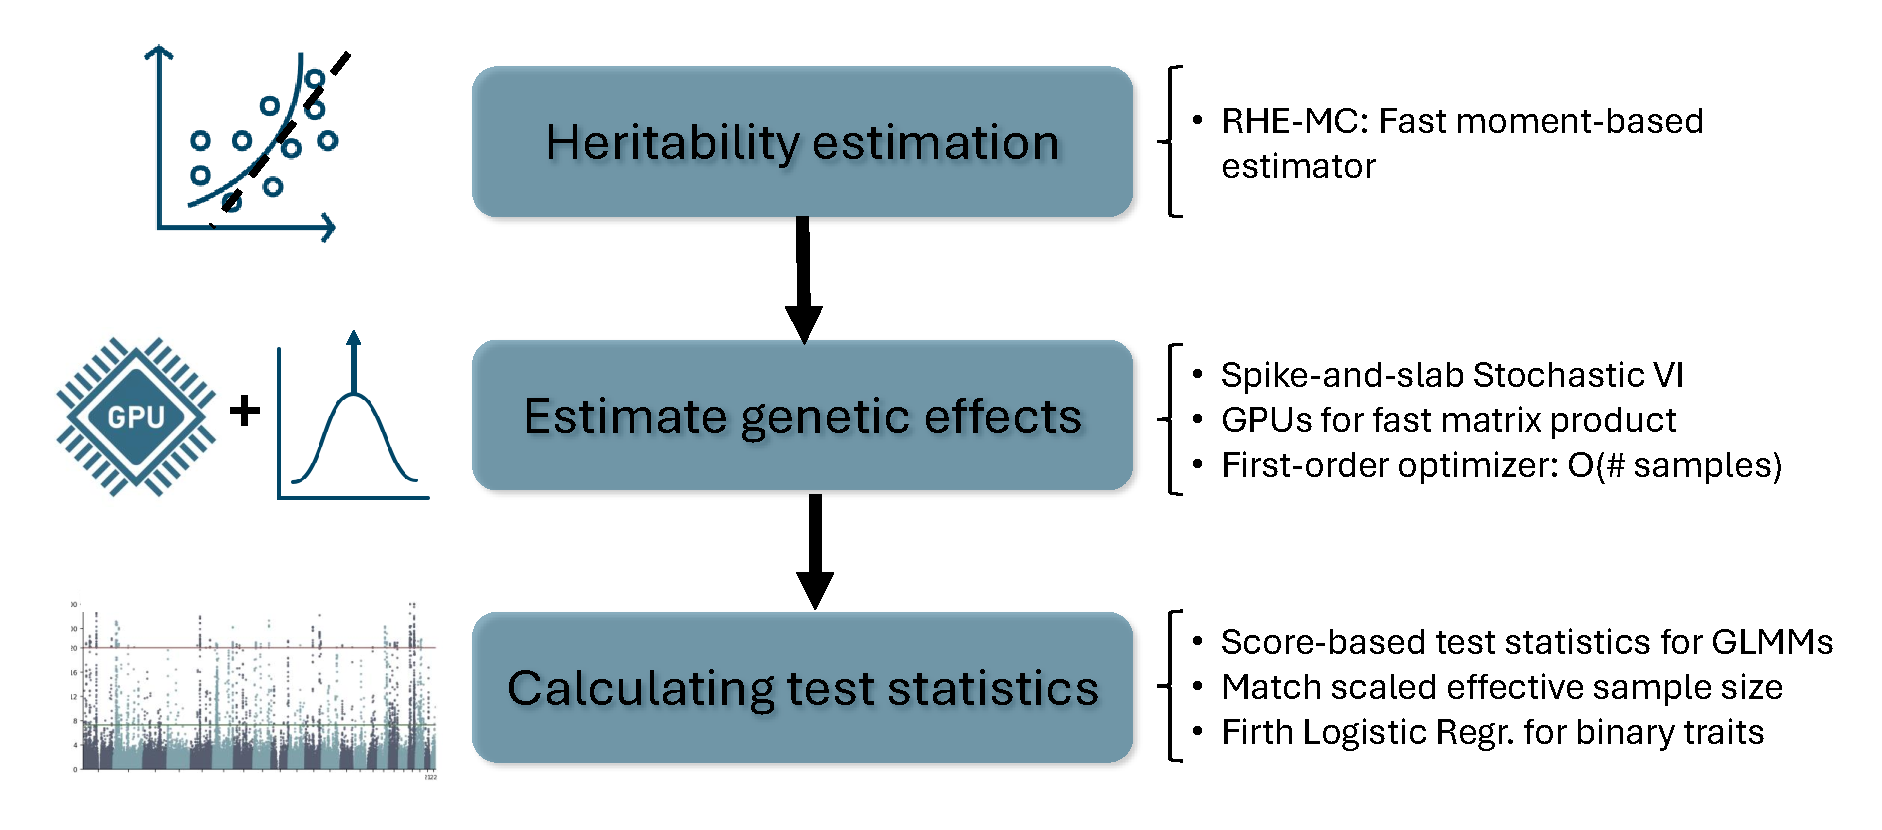
\includegraphics[width=\linewidth]{figures/thesis_qd_overview.pdf}
    \caption{\textbf{Overview of the Quickdraws algorithm.} The algorithm is divided into two main steps, first step deals with estimating genetic effects and the second step with calculating and calibrating per-variant test statistics. The first step is further divided into heritability estimation using moment-based methods \cite{zhu2024ARGRHE} and Bayesian regression for phenotype prediction which uses stochastic variational inference and GPU-based matrix multiplication for increased scalability. In the test statistics calculation step we use a novel calibration strategy which estimates and matches effective sample size with linear regression model run on unrelated and homogeneous subset of the data, along with approximate Firth logistic regression to correct for biases in binary traits. The illustrations were downloaded from Flaticon.}
    \label{fig:qd_overview}
\end{figure}

\subsection{Bayesian regression with spike-and-slab prior }
\label{sec:ch4-blr}
%
Quickdraws uses a Bayesian regression to estimate the genetic effects.
%
This Bayesian regression uses a spike-and-slab distribution on the variant effects, which results in increased association power compared to approaches that assume an infinitesimal model and rely on a Gaussian prior.
%
We optimize the posterior using stochastic variational inference \cite{hoffman2013stochastic}, which significantly improves the scalability of this approach.
%

\subsubsection{Quantitative traits}

Quickdraws adopts a Bayesian linear regression model as discussed in section \ref{sec:ch4-theory-mfvi}:
\begin{align}
    &\text{\textbf{Likelihood:} } &P(y \mid X, \beta) \sim \mathcal{N}(\beta^T X, \sigma_e^2) \nonumber \\
    &\text{\textbf{Prior:} } &P(\beta) = \prod_j P(\beta_j), \hspace{1mm} P(\beta_j) \sim (1-p_0)\mathcal{N} (0, \sigma ^ 2) + p_0 \delta(0) \nonumber \\
    &\text{\textbf{Approximate Posterior:} } &q(\beta) = \prod_j q(\beta_j), \hspace{1mm} q(\beta_j) \sim (1-\psi_j)\mathcal{N}(\mu_j, \sigma^2_j) + \psi_j \delta(0) \label{spike-and-slab-model2}
\end{align}

Similar to equation \ref{spike-and-slab-model}, given $N$ individuals and $M$ variants, $X$ is an $N \times M$ covariate-adjusted genotype matrix, $y$ is a $N \times 1$ covariate-adjusted phenotype vector, and $\beta$ is a $M \times 1$ vector of variant effects.
%
$\delta(0)$ is the Dirac delta function at 0, representing the spike in the spike-and-slab prior used to model the sparsity in the genetic architecture.
%
$\sigma_e^2$ and $\sigma^2$ are the variance component corresponding to environment and per predictor effect, $p_0$ is the sparsity and $j$ indexes over all model SNPs.
%
As we discussed in section \ref{sec:ch4-theory-mfvi}, we also assume a fully-factorized spike-and-slab approximate posterior, which leads to efficient and low-variance sampling from the posterior.
%
And, we use stochastic variational inference to directly optimize the evidence lower bound (ELBO).
%
The ELBO for Bayesian linear regression with spike-and-slab prior, normal likelihood, and spike-and-slab approximate posterior (derived in section \ref{sec:ch4-theory-svi}) can be approximated as follows: 
\begin{align}
    L^{Q}_{VI}&(\psi, \mu, \sigma) \approx - \sum\limits^{B}_{b=1} \Bigg( \sum\limits^{S}_{s=1} \frac{(y_b - \beta(s) X_b)^2}{2 \sigma_e^2} \ + \nonumber \\
    &+ \frac{1}{B}\sum\limits^{M}_{j=1} \left(  \frac{\psi_j}{2}\left(-1 + \frac{\mu_j^2 + \sigma_j^2}{\sigma^2} - \log \frac{\sigma_j^2}{\sigma^2} \right) + (1-\psi_j)\log\frac{1 - \psi_j}{1 - p_0} + \psi_j\log\frac{\psi_j}{p_0} \right) \Bigg) \label{elbo-loss-ss}
\end{align}

In this expression, $L^{Q}_{VI}(\psi, \mu, \sigma)$ is the variational inference objective to be maximized, $\psi, \mu, \sigma$ are the variational parameters to be optimized, $X_b$ and $y_b$ are a genotype matrix and a phenotype vector containing the $b^{th}$ (out of $B$) batch of the data, batched along the number of samples, while $\beta(s)$ are the effect estimates sampled from the approximate posterior $q(\beta)$.
%
Note that, contrary to other variational inference schemes, we aim to optimize a stochastic objective, since $\beta(s)$ is randomly sampled.
%

\subsubsection{Binary traits}
%
For binary traits, we adopt a Bayesian logistic regression model, so that the likelihood of Equation \ref{spike-and-slab-model2} becomes:
\begin{align}
    P(y \mid X, \beta) &= \prod_{n=1}^{N} c_n^{y_n} \{1 - c_n\}^{1-y_n}, \hspace{1mm} c_n = \sigma(\beta^T X_n),
    \label{spike-and-slab-model3}
\end{align}
while the prior and approximate posterior are unchanged.
%
In the above, $X_n$ and $y_n$ represent the covariate-adjusted genotype vector and phenotype values for the $n^{th}$ individual, $\sigma$ is the sigmoid function, which maps the output of the regression to a value between $0$ and $1$, and all other quantities are as previously defined.
%
We also assume that the approximate posterior has a spike-and-slab distribution; although it is not conjugate to the logistic distribution, we observed it to provide a good approximation to the true posterior.
%
The ELBO, which we again optimize using stochastic variational inference, now takes the form: 
\begin{align}
    L^{Bi}_{VI}&(\psi, \mu, \sigma) \approx - \sum\limits^{B}_{b=1} \Bigg( \sum\limits^{S}_{s=1} y_b \log(\sigma(\beta^T X_b)) + (1-y_b)\log(1-\sigma(\beta^T X_b)) \nonumber \ + \\
    &+ \frac{1}{B}\sum\limits^{M}_{j=1} \left(  \frac{\psi_j}{2}\left(-1 + \frac{\mu_j^2 + \sigma_j^2}{\sigma^2} - \log \frac{\sigma_j^2}{\sigma^2} \right) + (1-\psi_j)\log\frac{1 - \psi_j}{1 - p_0} + \psi_j\log\frac{\psi_j}{p_0} \right) \Bigg)
\end{align}

where all terms are defined as in Equation \ref{elbo-loss-ss} and derivation is provided in section \ref{sec:ch4-theory-svi}.

\subsubsection{Practical considerations}
Stochastic VI methods provide a principled and efficient way to perform variational inference.
%
This approach is simple but requires particular care to make sure that the variance of the ELBO estimate is not too large, as that may have a negative impact on convergence.
%
We make use of multiple recently developed strategies to reduce variance in the stochastic estimation of the ELBO, including continuous relaxation \cite{maddison2016concrete,jang2016categorical}, local reparameterization trick \cite{kingma2015variational}, and antithetic variates \cite{hammersley1956new}.

\vspace{2mm}

\noindent \textbf{Reparameterization:}
When dealing with stochastic objectives, such as the ELBO, it is often difficult to differentiate the objective due to intrinsic randomness in the parameters.
%
One solution to this problem is provided by the reparameterization trick \cite{kingma2013auto,blundell2015weight}, which models the stochasticity in the parameters as an input to the model rather than an intrinsic property of the model.
%
In more detail, the reparameterization trick assumes that distributions can be reparameterized in the form $g(\theta,\epsilon)$ where $\theta$ is the variational parameter, $\epsilon$ is the independently sampled random variable, and $g$ is a differentiable function.
%
As an example, consider the case of an isotropic normal distribution.
%
To sample from a mean-field normal distribution, we may reparameterize the sample as follows:
\begin{align}
    X &\sim \mathcal{N}(\mu, \sigma^2 I) \implies X = \mu + \epsilon \cdot \sigma, \nonumber \\
    \epsilon &\sim  \mathcal{N}(0, I),
\end{align}
where $\epsilon$ is i.i.d.\ normal noise with no dependence on $\mu$ and $\sigma$.
%
Relying on the reparameterization and treating $\epsilon$ as an independent input, we can differentiate with respect to $\mu$ and $\sigma$.
%

\vspace{2mm}
\noindent \textbf{Local reparamaterization:} The local reparamaterization trick \cite{kingma2015variational} was introduced as a way to provide computationally fast and low-variance gradient estimators in parameter-heavy stochastic VI methods.
%
It was originally applied to perform variational inference in Bayesian neural networks but is easily extended to Bayesian regression.
%
Using the original reparamaterization trick \cite{kingma2013auto,blundell2015weight} leads to sampling i.i.d.\ noise at least once for each parameter, making this approach computationally intensive in high-dimensional settings, which may involve millions of parameters.
%
The local reparamaterization trick translates the uncertainty on individual effect estimates, $\beta$, into local noise in the output, $\beta^T X$, thus reducing the computational overhead.
%
In the simple mean-field Gaussian VI, the local reparameterization trick can be used to sample the outputs directly,
\begin{align}
   &w_{i,j} \sim \mathcal{N}(\mu_{i,j}, \sigma^2_{i,j}), \hspace{4mm} b_{m,j} =  \sum_{i} a_{m,i} w_{i,j},
\end{align}
where $a_{m,i}$ is the $m$-th input data point and $b_{m,j}$ is the output corresponding to the $m$-th data point in the Bayesian linear regression model.
%
$b_{m,j}$ is a weighted-sum of normally distributed random variables, implying that $b_{m,j}$ is also normally distributed, with the following parameters:
\begin{align}
    &w_{i,j} \sim \mathcal{N}(\mu_{i,j}, \sigma^2_{i,j}) \implies b_{m,j} \sim \mathcal{N}(\gamma_{m,j}, \delta^2_{m,j}), \nonumber \\
    &\gamma_{m,j} = \sum_{i}a_{m,i}\mu_{i,j} ,\hspace{4mm}\delta^2_{m,j} =  \sum_{i}a^2_{m,i}\sigma^2_{i,j}.
\end{align}

In order to sample this output directly, one can apply the original reparameterization trick for the normal distribution:
\begin{align}
   b_{m,j} =  \gamma_{m,j} + \epsilon_{m,j} \delta_{m,j}, \hspace{4mm} \epsilon_{m,j} \sim \mathcal{N}(0, 1).
\label{eq:reparam_local}
\end{align}

Note that in Bayesian linear/logistic regression the local reparameterization removes the need to sample all the weights in a layer and only requires sampling proportional to the number of output variables for each mini-batch of data, substantially improving the computational complexity of the algorithm.
%
% Its important to note in Bayesian linear/logistic regression and Bayesian neural networks, the local reparameterization reduces sampling all the weights in the layer - $\mathcal{O}(N^2)$ to only sampling the pre-activations - $\mathcal{O}(N)$.

%
The local reparamaterization trick was originally only derived for mean-field Gaussian variational inference, since the weighted sum of arbitrary distributions cannot always be analytically derived.
%
In the case of mean-field spike-and-slab distributions, we use the central limit theorem to approximate the weighted sum of independent spike-and-slab distributions as approximately Gaussian.
%
Note that the input dimension for Bayesian regression in our setup is quite high (usually $>100,000$ markers), justifying this approximation.
%
% Thus, the central limit theorem provides a close approximation to the output of the model.
This idea was first explored in \cite{shayer2017learning} to sample discrete weights for binary and ternary neural networks.
% , relying on Lyapunov central limit theorems.
%
We thus reparametrize the output of our model (as described in equations \ref{spike-and-slab-model2} and \ref{spike-and-slab-model3}) as follows:
\begin{align}
    w_{i,j} &\sim p_{i,j}\mathcal{N}(\mu_{i,j}, \sigma^2_{i,j}) + (1 - p_{i,j})\delta(0) \implies b_{m,j} \sim \mathcal{N}(\gamma_{m,j}, \delta_{m,j}),  \nonumber \\
    \gamma_{m,j} &= \sum_{i}a_{m,i}\mu_{i,j}p_{i,j} ,\hspace{4mm}\delta_{m,j} =  \sum_{i}a^2_{m,i}(p_{i,j}\sigma^2_{i,j} + p_{i,j}\mu^2_{i,j} - p^2_{i,j}\mu^2_{i,j}).
\end{align}


\vspace{2mm}
\noindent \textbf{Antithetic variates for variance reduction:}
%
The use of antithetic variates is a popular approach to speed up Monte Carlo computations of the expectation of a random function \cite{hammersley1956new}.
%
This strategy relies on taking the antithetic path of the sampled path to reduce the variance in the overall estimator.
%
For example, in order to sample from a normal random variable (with mean $\mu$ and variance $\sigma^2$), one might use the reparameterization trick to sample $\mu +\epsilon \sigma$.
%
The antithetic path for a normally distributed random variable is $\mu - \epsilon \sigma$.
%
In addition to providing a valid sample from the underlying distribution (in this case, normal with mean $\mu$ and variance $\sigma^2$), the antithetic path also reduces the variance of the Monte Carlo estimate, as the sampled path and antithetic path are often negatively correlated.
%

%
We use both antithetic variates and the local reparameterization trick to reduce the variance of the ELBO.
%
As described above, the antithetic path for a normally distributed random variable is simply obtained by replacing $\epsilon$ with $-\epsilon$.
%
For each forward pass, we thus obtain two Monte Carlo samples for the output of the model as follows: 
\begin{align}
    \beta(s_1) &=  (\sum_{i}a_{m,i}\mu_{i,j} + \sqrt{\sum_{i}a^2_{m,i}(p_{i,j}\sigma^2_{i,j} + p_{i,j}\mu^2_{i,j} - p^2_{i,j}\mu^2_{i,j}} \epsilon ), \nonumber \\
    \beta(s_2) &= (\sum_{i}a_{m,i}\mu_{i,j} - \sqrt{\sum_{i}a^2_{m,i}(p_{i,j}\sigma^2_{i,j} + p_{i,j}\mu^2_{i,j} - p^2_{i,j}\mu^2_{i,j}} \epsilon ), \nonumber \\
    \beta(s) &= [\beta(s_1), \beta_2(s_2)].
\end{align}

\subsection{Heritability estimation}
\label{methods:h2}
%
To set the prior variance and likelihood contribution in equations \ref{spike-and-slab-model2} and \ref{spike-and-slab-model3}, we compute an estimate of the narrow-sense heritability for the trait of interest.
%
For quantitative traits, we estimate heritability using a parallelized implementation of the randomized Haseman–Elston regression algorithm\cite{wu2018scalable,pazokitoroudi2020efficient} (RHE, PyPI version 1.0) that allows the simultaneous estimation of variance components for multiple traits \cite{zhu2024ARGRHE}.
%
This approach requires a single pass through the data and allows estimating heritability in time linear in $N$ and $M$.
%
We set the number of random RHE-mc vectors to $50$ while assigning markers to $8$ components based on their LD scores and MAF. 
%
We also exclude the HLA region, as recommended in \cite{pazokitoroudi2020efficient}.
%
For Binary traits, we perform a grid search over a set of heritability values, $h2 \in \{0.01, 0.25, 0.5, 0.75\}$, running the Bayesian regression for each value and selecting the heritability corresponding to the highest likelihood.
%


\subsection{Test statistics calculation}
\label{methods:test_stats}
% talk about step1, now we do step 2
%
After estimating the random genetic effects as described in sections \ref{sec:ch4-blr} and \ref{methods:h2}, we compute association statistics for quantitative or binary traits as follows.
%
\subsubsection{Quantitative traits} 
%
We model the phenotype of interest as a combination of fixed and random effects, which include genetic effects and environmental effects:
\begin{equation}
    y = \alpha C + x_{test}\beta_{test} + g + \epsilon, \label{eq:lin_lmm}
\end{equation}
where $y$ is a $N \times 1$ vector of phenotype values, $x_{test}$ is a $N \times 1$ vector of variant values, $C$ is a $N \times C$ matrix of C covariates, $g$ and $\epsilon$ are random genetic and environmental effects.
%
Note that using a covariate-adjusted genotype and phenotype by first regressing out any covariates is equivalent to including covariates as fixed effects in the above equation.
%
Based on this model, we aim to compute the following $\chi^2$ association statistic (a derivation is provided in section \ref{sec:ch1-lmm}): 
\begin{equation}
   \frac{(x_{test}^T \hat{V}^{-1} y)^2}{x_{test}^T \hat{V}^{-1} x_{test}} \sim \chi^2_1, \label{lmm-chi2}
\end{equation}
where $\hat{V}$ is the estimated variance matrix, defined as $\hat{V} = \frac{\hat{\sigma_g}^2}{M} X_{GRM}X_{GRM}^T + \hat{\sigma_e}^2 I_N$, $\hat{\sigma_g}^2$ and $\hat{\sigma_e}^2$ are estimated genetic and environmental variance components, and $X_{GRM}$ is the genotype matrix used for model fitting.
%
Obtaining the test statistic of Equation \ref{lmm-chi2} requires calculating the inverse of a $N \times N$ matrix, which creates a computational bottleneck for large sample sizes.
%
This test statistic can be linked to the best linear unbiased predictor (BLUP) of a trait, by re-writing Equation \ref{lmm-chi2} as described in \cite{loh2015efficient}:
\begin{equation}
    \frac{(x_{test}^T \tilde{y}/\sigma_e^2)^2}{x_{test}^T \hat{V}^{-1} x_{test}} \sim \chi^2_1.
    \label{blup_lmm}
\end{equation}

%
In the above, $\tilde{y}$ is a residual phenotype estimated using BLUP.
%
We adopt a similar strategy and replace the $\tilde{y}$ with $\tilde{y}_{LOCO}$, leave-one-chromosome-out residual phenotype from Bayesian regression.
%
In addition, the denominator $x_{test}^T \hat{V}^{-1} x_{test}$ of Equation \ref{blup_lmm} can be shown to be well approximated using a constant multiple of $x_{test}^T x_{test}$ \cite{svishcheva2012rapid}, further reducing computational costs.
%
We can therefore write the test statistics for a quantitative trait up to a constant of proportionality as:
\begin{equation}
    \chi^2_{Q} \propto \frac{(x_{test}^T \tilde{y}_{LOCO})^2}{x_{test}^T x_{test}}.
    \label{chisq_test_2}
\end{equation}

\subsubsection{Binary traits}
%
For binary traits, we model the association between genotype and phenotype using a logistic mixed model:
\begin{equation}
    logit(p_i) = \alpha C + x_{test}\beta_{test} + g + \epsilon, \label{eq:log_lmm}
\end{equation}
where $p_i = P(y_i = 1 \mid x_{test}, g, C)$ is the probability of $i^{th}$ individual being a case given $x_{test}$, covariates $C$, and random genetic effects $g$.
%
A score test statistic for the null hypothesis $\beta_{test} = 0$ is then computed as $T = x_{test}^T(y - \hat{p})$, where $\hat{p}$ is the estimated mean under the null model.
%
The normalized test statistic for logistic mixed model can then be written as: 
\begin{equation}
    T = \frac{x_{test}^T(y - \hat{p})}{\sqrt{x_{test}^T\hat{P}x_{test}}},
\label{eq:log_lmm1}
\end{equation}
where $\hat{P} = \hat{V}^{-1} - \hat{V}^{-1} C(C^T\hat{V}^{-1}C)^{-1}C^T\hat{V}^{-1}$ is a dense $N \times N$ matrix with $\hat{V} = \frac{\hat{\sigma_g}^2}{M} X_{GRM}X_{GRM}^T + \hat{W}^{-1}$ and $\hat{W} = diag\{ \hat{p} (1-\hat{p}) \}$.
%
Similar to quantitative traits, the test statistic in Equation \ref{eq:log_lmm} can be written up to a constant of proportionality \cite{zhou2018efficiently} as:
\begin{equation}
    T_{B} \propto \frac{x_{test}^T(y - \hat{p})}{\sqrt{x_{test}^T\hat{W}x_{test}}},
\label{eq:log_lmm2}
\end{equation}
where $\hat{W}$ is a diagonal matrix (with diagonal entries $\hat{p_i} (1-\hat{p_i})$) from the predictions of the null model in Step 1.
%
The test statistic from \ref{eq:log_lmm2} is assumed to be normally distributed, which is often not the case with binary traits that have low prevalence or for rare variants.
%
We therefore instead perform Firth logistic regression, which penalizes the likelihood by using a Jeffreys' prior, removing most of the asymptotic bias in maximum-likelihood estimation.
%
In order to save computation, we use the likelihood ratio test with an approximate version of Firth logistic regression introduced in \cite{mbatchou2021computationally} on variants below a p-value threshold of 0.05. 
%
We further narrow down the list of variants by only applying Firth logistic regression to rare variants (default MAF $< 5\%$) or rare traits (default prevalence $< 5\%$) or both.

\subsubsection{Calibration of test statistics}

Calibrating the test statistics generated upto a constant of proportionality in equation \ref{chisq_test_2} and \ref{eq:log_lmm2} is a crucial part of a GWAS algorithm, which ensures the false positives are controlled.
%
We calibrate the summary statistics by estimating the effective sample size (ESS) increase compared to running linear regression on a homogeneous subset of unrelated individuals.
%
To this end, we estimate the increase in ESS linked to the use of non-infinitesimal Bayesian linear regression ($\gamma_{blr}$), as well as the reduction in ESS due to the presence of close relatives ($\gamma_{rel}$).
%
We then adjust the summary association statistics by matching the mean $\chi^2$ statistic minus one \cite{yang2011genomic} with that observed for linear or logistic regression run on a homogeneous subset of unrelated individuals.
%
In more detail, we multiply the uncalibrated Quickdraws summary statistics from equations \ref{chisq_test_2} and \ref{eq:log_lmm2} by a correction term $c$, computed as:
\begin{equation}
c = \frac{\gamma_{rel}\gamma_{blr}\frac{N_{qd}}{N_{lr}}(<\chi_{lr}^2> - 1) + 1}{<\chi_{qd}^2>}.
\label{eq:calib_main}
\end{equation}
In the above, $<\chi_{qd}^2>$ and $<\chi_{lr}^2>$ are the mean $\chi^2$ test statistics from Quickdraws and from linear/logistic regression run on a homogeneous unrelated subset of individuals, respectively.
%
$\frac{N_{qd}}{N_{lr}}$ is the ratio of the total number of samples to the number of homogeneous unrelated samples used for linear/logistic regression.
%
$\gamma_{rel}$ and $\gamma_{blr}$ are correction terms to account for relatedness and the use of Bayesian linear regression, which we describe in detail below.
%
Note that the $\gamma_{blr}$ term is estimated for each LOCO run, so the correction in equation \ref{eq:calib_main} is performed separately for each chromosome.
%
For binary traits, we use logistic regression and apply the correction separately for Firth-corrected and Firth-uncorrected variants.

\vspace{2mm}

%
\noindent \textbf{Correcting the ESS for the presence of relatedness ($\gamma_{rel}$ term).} To estimate the effective number of samples in the presence of relatedness, we follow an approach similar to that of \cite{ziyatdinov2021estimating}.
%
To this end, we first estimate genetic relatedness between samples using KING \cite{manichaikul2010robust} as implemented in PLINK \cite{chang2015second}.
%
We only retain relationships up to the 3rd degree (KING score $>2^{-\frac{9}{2}}$), as we found the ESS multiplier, described below, to not be significantly impacted by the inclusion of higher degree relatives.
%
For each pair of relatives, we estimate the degree of the relationship using KING’s output values as follows:

\begin{table}[h!]
\centering
\begin{tabular}{|c|c|}
\hline
\textbf{Range for KING $\psi$ value} & \textbf{Relatedness} \\
\hline
$\psi \geq 2^{-\frac{3}{2}}$ & 1 (Monozygotic Twins) \\
$2^{-\frac{3}{2}} > \psi \geq 2^{-\frac{5}{2}}$ & 0.5 ($1^{\text{st}}$ degree) \\
$2^{-\frac{5}{2}} > \psi \geq 2^{-\frac{7}{2}}$ & 0.25 ($2^{\text{nd}}$ degree) \\
$2^{-\frac{7}{2}} > \psi \geq 2^{-\frac{9}{2}}$ & 0.125 ($3^{\text{rd}}$ degree) \\
\hline
\end{tabular}
\caption{\textbf{Genetic relationship estimates based on KING values.}}
\label{tab:my_label}
\end{table}

Based on this, we compute the reduction factor for the effective sample size, $\gamma_{rel}$, using the following estimator, for which a derivation can be found in \cite{ziyatdinov2021estimating}:
\begin{equation}
\gamma_{rel} = \frac{tr((K \sigma_g^2 + I (1-\sigma_g^2))^{-1}K)}{N}.
\label{eq:calib_rel}
\end{equation}
In this expression, $N$ is the total number of samples, $K$ is the estimated kinship matrix, and $\sigma_g^2$ is the heritability of the trait.
%
To efficiently compute $\gamma_{rel}$, we eigendecompose the matrix $K$, obtained using KING utilizing the block-like structure of the kinship matrix. 
%
In particular, the effective sample size multiplier in the presence of relatedness can be approximated as:
\begin{equation}
\gamma_{\text{rel}} \approx \frac{1}{N}\sum\limits_{i=1}^{N} \frac{\lambda_i}{(\lambda_i - 1)\sigma_g^2 + 1},
\end{equation}
where $\lambda_i$ is the $i^{\text{th}}$ eigenvalue of the kinship matrix $K$.
%
And to facilitate this computation, we separately sum across each block $B_i$ of related individuals:
\begin{equation}
\gamma_{\text{rel}} \approx \frac{1}{N} \sum\limits_{i=1}^{B} \sum\limits_{j=1}^{N_{B_i}} \frac{\lambda_{i,j}}{(\lambda_{i,j} - 1)\sigma_g^2 + 1}.
\end{equation}
%
For binary traits, we convert the heritability from the liability scale to the observed scale.
%

\vspace{2mm}

%
\noindent \textbf{Correcting the ESS for the use of Bayesian linear regression ($\gamma_{blr}$ term):}
%
The effective sample size multiplier, $\gamma_{blr}$, has been shown to be proportional to the inverse of the residual trait variance in a linear regression model \cite{loh2015efficient, ziyatdinov2021estimating}.
%
To account for the increase in effective sample size in the model fitting step, we therefore calculate the inverse variance of the residual trait 
\begin{equation}
    \gamma_{blr} = \frac{Var(y)}{Var(y-\hat{y})}
\end{equation}
where $y$ and $\hat{y}$ are true and predicted trait values from the whole-genome regression regression on a held-out set.
%
In more detail, we use the effect estimates from the best sparsity parameter to calculate the variance explained on held-out data.
%
As the $\gamma_{blr}$ term needs to be computed during the LOCO step, we compute these variance terms separately for each chromosome and sum across all chromosomes, excluding the one currently being tested.
%


\subsection{Performance optimization}
\subsubsection{Memory optimization}
\begin{enumerate}
    \item \textbf{Raw genotypes:}
    %
    for a diploid individual, the raw genotypes take values in ${0,1,2}$.
    %
    We store the $N \times M$ genotype matrix in $NM/4$ bytes, i.e. using 2 bits per genotype entry.
    %
    We do so by encoding 8 consecutive entries of the genotype matrix using two 8-bit integers using the built-in \texttt{numpy} features in Python, \texttt{np.packbits()} and \texttt{np.unpackbits()}.
    %
    We also store the column-wise mean and variance of the genotype matrix, used to mean-center and standardize, on the fly.
    %
    
    \item \textbf{Genotype streaming during the calculation of test statistics:}
    %
    the calculation of test statistics is usually performed on many more variants than those used for model fitting.
    %
    We therefore optimize this step by streaming genotype blocks rather than loading all the variants into memory.
    %
    The block size is determined based on the maximum memory allowed at runtime (default: 32GB) and the data IO is parallelized using multiple cores.
    %
    
\end{enumerate}

%% Handle raw genotypes, saved in HDF5 file for speedy access
%% Streaming genotype rathern than loading it
\subsubsection{Speed optimization}
\begin{enumerate}
    \item \textbf{GPUs for fast Bayesian regression:} we use GPUs along with the \texttt{pytorch} machine learning package \cite{paszke2017automatic} to speed-up matrix multiplication and sampling operations during stochastic variational inference.
    %
    % We observed by using GPUs we were able to speed-up the matrix multiplication and sampling bottlenecks thereby making our Bayesian regression much faster than just using CPUs. 
    % We benchmark the speed gain in whole-genome regression and compare on two popular GPU models: Nvidia A100 and Nvidia 3080.  
    % Add figure comparing performance gain due to using GPUs vs CPUs
    \item \textbf{Transfer learning:} rather than training the $22$ LOCO models independently, we initialize each model training using the effect estimates previously computed for the whole-genome regression.
    %
    This transfer learning approach requires fewer iterations to converge, making model fitting $2\times$ to $2.5\times$ faster, and leads to similar association power when compared to training each LOCO model separately.
    %
    We compare the advantage of transfer learning over independent random initialization in simulations, by looking at the power improvement vs number of iterations in Figure \ref{fig:transfer}.

    \begin{figure}[h]
    \centering
    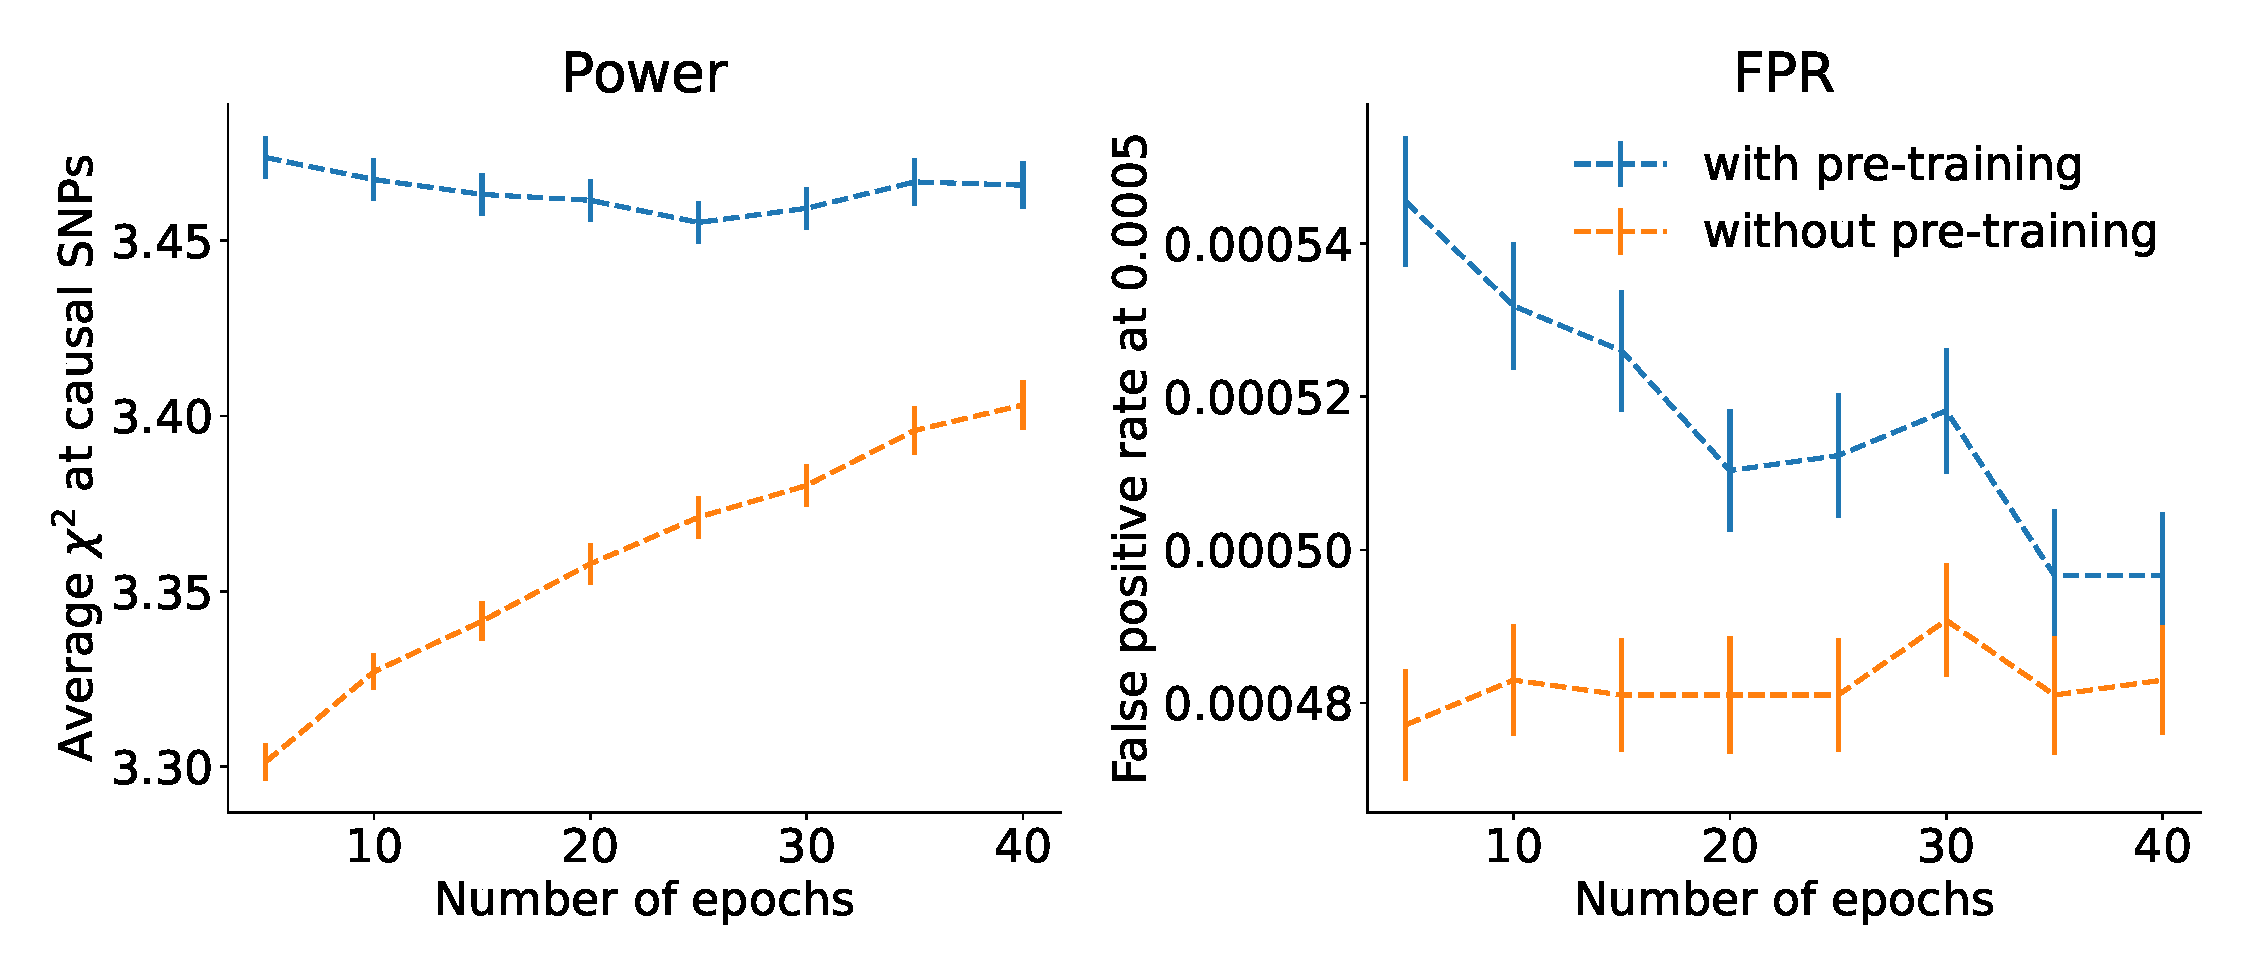
\includegraphics[width=\textwidth]{figures/transfer.pdf}
    \caption{\textbf{
    %
    Transfer-learning in Bayesian regression.}
    %
    We measure the causal $\chi^2$ and false positive rate at $5 \times 10^{-4}$, with and without pre-training (for $90$ epochs), and varying the number of LOCO training epochs.
    %
    Error bars represent the standard error of the mean $\chi^2$ or false positive rate across $50$ independent quantitative traits with GB-unrel structure and $2\%$ polygenicity.
    %
    }
    \label{fig:transfer}
\end{figure}
    

    \item \textbf{Numba optimization for the calculation of test statistics:}
    %
    we implement a fully-vectorized version of linear regression for multiple traits using the \texttt{parallel} and \texttt{njit} functionality from the Numba just-in-time (JIT) compiler \cite{lam2015numba}.
    %
    % Numba is able to escape the global interpreter lock in python, making the code able to compile without involving any interpreter - this along with prebuilt numpy features makes the python code as fast as a C or C++ implementation of it. 
    \item \textbf{Calibrating test statistics using genotyped SNP data:}
    %
    instead of running linear regression or logistic regression on all imputed variants, we calibrate our test statistics only using the genotype data provided in step 1 (${\sim}458k$ variants).
    %
    We find that matching scaled effective sample size estimates using this subset of variants provides consistent calibration in the larger set of imputed variants, while greatly reducing running time, as we only need to evaluate the logistic or linear regression model on a subset of variants.
    %
    \item \textbf{HDF5 and PySnpTools for data loading:}
    %
    we store the raw genotype matrix in a compressed HDF5 file \cite{hdf5}, which provides fast sample-wise access (i.e., it allows obtaining all variants for an individual) for Bayesian regression.
    %
    We instead use PySnpTools (see \url{https://github.com/fastlmm/PySnpTools}), which provides parallelizable variant-wise access, to access \texttt{bgen} or \texttt{bed} files for the calculation of test statistics. 
    \item \textbf{Approximate Firth logistic regression:} Approximate Firth regression is only applied to variants with logistic regression p-value below $0.05$, as done in Regenie and FastGWA-GLMM.
    %
    We further narrow down the list of variants by only applying Firth logistic regression to rare variants (MAF < 5\%) or rare traits (prevalence < 5\%).
    %
    \item \textbf{Multiple traits:} Most of our operations are vectorized using Numpy \cite{harris2020array} and Numba \cite{lam2015numba}, which leads to computational gains in the parallel analysis of multiple traits.
    %
\end{enumerate}

\subsection{Hyperparameter tuning}
We perform cross-validation by randomly splitting the data into training ($80\%$) and testing ($20\%$) sets to estimate the optimal sparsity hyperparameter $1-p_0$ (see Equation \ref{spike-and-slab-model}) using the values $\{0.5, 0.2, 0.1, 0.05, 0.02, 0.01\}$.
%
For heritability in binary traits, we evaluate $\{0.01, 0.25, 0.5, 0.75 \}$.
%
Compared to coordinate-ascent variational inference, stochastic variational inference relies on additional hyperparameters that affect the final testing performance.
%
These include the learning rate of the optimizer, the batch-size, and the number of training epochs.
%
Setting a high learning rate results in unstable convergence of the optimizer, while a low learning rate leads to the need for more training epochs.
%
Larger batch sizes lead to better performance but increased GPU memory usage.
%
Considering these trade-offs, we set the batch-size to $128$; the learning rate corresponding to each value of the sparsity hyperparameter was set to $4 \times 10^{-4}$, $2 \times 10^{-4}$, $2 \times 10^{-4}$, $1 \times 10^{-4}$,$2 \times 10^{-5}$, $5 \times 10^{-6}$ for sparsity ($1-p_0$) $ \in \{0.01, 0.02, 0.05, 0.1, 0.2, 0.5\}$.
%
We also set the number of training epochs to $80$ for the initial cross-validation step, and to $40$ for the final LOCO step.
%
We observed these hyperparameters to be robust across various sample sizes, providing a good balance between statistical power and computational costs. 

\newpage

\section{Summary of the Quickdraws algorithm}
\label{sec:ch4-summary}
%
We provide a summary of the Quickdraws algorithm, which performs two main steps:
%
\begin{enumerate}
    \item \textbf{Estimating genetic effects (model fitting):} This is further divided into two parts:
    \begin{enumerate}
        \item \textbf{Variance component estimation:}
        %
        For quantitative traits, we use a multi-trait version of the RHE-mc algorithm \cite{wu2018scalable,pazokitoroudi2020efficient,zhu2024ARGRHE} to obtain estimates of narrow-sense heritability.
        %
        For binary traits, we directly perform the Bayesian regression (see below) while testing several heritability values in a grid search.
        %
        \item \textbf{Bayesian regression: }
        %
        We perform Bayesian linear/logistic regression to estimate the genetic effects, using a spike-and-slab prior on the effect estimates:
        \begin{equation}
            P(\beta_j) \sim (1-p_0)\mathcal{N} (0, \sigma ^ 2) + p_0 \delta(0).
        \end{equation}
        
        %
        There is one free hyperparameter in the prior (the sparsity term $1-p_0$) for quantitative traits and two free hyperparameters for binary traits (the sparsity term and $h^2$).
        %
        We perform cross-validation to estimate these hyperparameters, splitting the input genotype/phenotype data into $90\%$ for training and $10\%$ for validation and parallelly running the regression using $1-p_0 \in \{0.01, 0.02, 0.05, 0.1, 0.2, 0.5\}$ and, for binary traits, $h^2 \in \{0.01, 0.25, 0.5, 0.75, 0.9 \}$.
        %
        We choose the sparsity (and $h^2$ for binary traits) parameter that maximizes (in the validation set) the test log-likelihood for the traits.
        %

        %
        After obtaining the optimal hyperparameters for each trait, we retrain the regression using a leave-one-chromosome-out approach.
        %
        We obtain a $2.5-3 \times$ speed-up for the training for this LOCO step by using transfer learning, initializing the effect estimates from the cross-validation run performed using all chromosomes.
        %
    \end{enumerate}
    %    
    \item \textbf{Calculation and calibration of association statistics (testing):}
    %
    Given the estimated genetic effects, we calculate linear mixed-model or logistic mixed-model test statistics up to a constant of proportionality.
    %
    We rely on optimizations such as just-in-time compilation and code vectorization in Numba.
    %
    We estimate the constant of proportionality by matching the estimated scaled effective sample size of linear regression on a subset of unrelated homogeneous samples for quantitative traits, and logistic regression on a subset of unrelated homogeneous samples for binary traits.
    %
\end{enumerate}
\chapter{\label{ch:5-qd-result}Application to simulated and real phenotypes in UK Biobank}

\minitoc

\section{Chapter overview}

In this chapter we apply Quickdraws to simulated and real phenotypes in the UK Biobank \cite{bycroft2018uk}. We start by discussing data and quality control steps we used to perform GWAS in the UK Biobank in section \ref{sec:ch5-data}. In order to assess the calibration and demonstrate statistical power we then perform simulation studies in section \ref{sec:ch5-sim} across a wide variety of designs varying relatedness, population structure, prevalence and the genetic architecture of the simulated trait. Subsequently in section \ref{sec:ch5-ukb}, we apply Quickdraws on 79 quantitative and 50 self-reported disease phenotypes from UK Biobank where we show Quickdraws leads to state-of-the-art statistical power while controlling for false positives. We perform a replication analysis with summary statistics from external biobanks like Biobank Japan and Finngen, followed by predictive power analysis and comparing with PGS methods. Finally in section \ref{sec:ch5-cost}, we perform a thorough cost analysis on UK Biobank's cloud platform comparing Quickdraws against recent scalable methods like FastGWA and Regenie. We conclude the chapter with discussing the key findings and directions for future work.

\section{Data and quality control}
\label{sec:ch5-data}

\subsection{UK Biobank data}

We used the UK Biobank SNP array data for $405{,}088$ white British samples \cite{bycroft2018uk} (in PLINK bed format \cite{purcell2007plink,chang2015second}) for model fitting and HRC+UK10k-imputed data \cite{haplotype2016reference,uk10k2015uk10k,bycroft2018uk} (in bgen v1.2 format \cite{band2018bgen}) for association testing.
%
We filtered the set of available autosomal variants to have minor allele frequency (MAF) $\geq 1\%$, Hardy-Weinberg equilibrium $p \geq 1 \times 10^{-15}$, and a genotyping rate above $99\%$, obtaining a set of $458{,}620$ markers.
%
We used these markers as input for the model-fitting step of BOLT-LMM, Regenie, and Quickdraws, while for Saige we performed LD pruning using PLINK (v1.9 \cite{purcell2007plink,chang2015second} setting \texttt{--window\_size} to 50kb, \texttt{--step\_size} to 5, and the $R^2$ threshold to $0.05$) as recommended, which resulted in $89,177$ markers.
%
We computed association statistics on a much larger set of ${\sim}13.3$ imputed variants with MAF $\geq 0.1\%$ and INFO score $\geq 0.8$.
%

%
For our main analyses we considered $79$ quantitative traits (comprising blood-related, anthropometric, and other traits) and $50$ binary self-reported disease traits.
%
The traits we selected had a phenotyping rate higher than $80\%$ and, for quantitative traits, a statistically significant estimated narrow-sense heritability ($p < 5 \times 10^{-4}$, using LD-score regression estimates available at \url{https://nealelab.github.io/UKBB_ldsc/h2_browser.html}).
%
Quantitative traits were also standardized, mean-centered, and quantile normalized to have an approximately Gaussian distribution.
%
All methods we considered were provided with the top $20$ principal components \cite{bycroft2018uk}, $age$, $sex$, $age^2$, $age*sex$, $age^2*sex$, and smoking status as covariates during model fitting and testing.
%

We additionally considered $2{,}923$ plasma protein traits from the UK Biobank, which we pre-processed as done in \cite{sun2023plasma, dhindsa2023rare}.
%
We downloaded normalized protein expression values from the UK Biobank RAP (field $30900$), with measurements for up to $53{,}074$ participants.
%
For GWAS, we considered up to $49{,}441$ European participants (based on self-reported field $21000$).
%
We ran Quickdraws with covariates including the top $20$ principal components \cite{bycroft2018uk}, $age$, $sex$, $age^2$, $age*sex$, $age^2*sex$, smoking status, collection site, batch, and time difference between blood sampling and protein measurement.
%
We also ran Regenie on $250$ randomly sampled plasma proteins, focusing on a subset of $N=43{,}293$ individuals overlapping the British ancestry subgroup described in \cite{bycroft2018uk}.
%
Association was performed in independent batches of $250$ traits in parallel.

\subsection{Quality control and preprocessing for GWAS}
Our analyses made use of the following filtering criteria:
\begin{enumerate}
    \item \textbf{Genotype QC:} for model fitting, we use markers with minor allele frequency $\geq$ 1\%, Hardy-Weinberg equilibrium test $P > 1 \times 10^{-15}$, and genotyping rate $> 99\%$. 
    \item \textbf{Missing data:} we remove samples with phenotype missingness above 50\% and mean-impute the remaining missing values.
    %
    During the Bayesian regression step, we also median-impute the genotype matrix to enable 2-bit genotype encoding. We allow missing data during the computation of test statistics.
    \item \textbf{Mean-centering and transforming:} all analyses are performed on mean-centered and standardized genotypes.
    %
    Quantitative phenotypes are mean centered, and quantile normalized to a normal distribution.
    \item \textbf{Covariates:} we regress covariates (top $20$ PCs, age, sex, age$^2$, age$\times$sex, age$^2\times$sex, smoking status) from both genotype and phenotype on the fly, which is equivalent to including covariates as fixed effects in the model.
    %
    We also remove individuals with any missing covariates (`complete case analysis').
\end{enumerate}

\section{Performance in simulated data}
\label{sec:ch5-sim}

\subsection{Simulation design}
\label{sec:ch5-sim-design}
To assess the robustness and power of Quickdraws and other methods, we performed simulations with varying levels of relatedness and population stratification.
%
We used SNP array data from the UK Biobank, using all autosomal variants with minor allele frequency $\geq 0.01\%$, Hardy-Weinberg equilibrium $p \geq 1 \times 10^{-15}$, and a genotyping rate above $99\%$, obtaining $512,828$ variants.
%
Of these, $54{,}568$ had a minor allele frequency (MAF) between $10^{-4}$ and $10^{-2}$.
%
We either randomly sampled $50{,}000$ individuals to assemble groups of samples matching specific relatedness and population structure criteria, or considered the entire subset of white British individuals (N=$405k$).
%
In each setting, we simulated $50$ quantitative and $50$ binary traits with narrow-sense heritability $h_g^2 = 0.4$, a realistic MAF dependence ($\alpha = -0.3$ \cite{zeng2018signatures,schoech2019quantification}), and varying polygenicity and prevalence levels.
%

%
We also simulated phenotypes generated using different distributions of genetic effects, including spike-and-slab, mixture of Gaussians, Laplace, and Gaussian.
%
To simulate effects following a spike-and-slab prior, given a polygenicity value $p$ and $M$ variants, we randomly selected $Mp$ causal variants (out of $M = 512,828$ variants) and randomly sampled their effect sizes from a Gaussian distribution. 
%
To facilitate the calculation of false positive rates and assess calibration, we only chose causal variants from the odd chromosomes, setting the effect sizes of variants on even chromosomes to zero.
%
We simulated population stratification and shared environment between close relatives using
%

\begin{align}
    y_i &= \sum\limits_{j=1}^{Mp} G_{i,j}\beta_j + A\gamma + \tau + \epsilon,  \nonumber \\
    \beta_j &\sim \mathcal{N}(0, \frac{h_g^2 c_f}{Mp}) \hspace{5mm} \epsilon \sim \mathcal{N}(0, h_e^2),
\label{eq:sim_gen}
\end{align}

%% insert figure about simulation

where $\sum\limits_{j=1}^{Mp} G_{i,j}\beta_j$ is a genetic effect explaining $40\%$ of trait variance, $A\gamma$ is a population stratification term determined using self-reported ancestry, $\tau$ is the shared environmental effect, simulated by assigning a Gaussian draw to closely related individuals, and $\epsilon$ is the residual environmental effect, with variance equal to $h^2_e$.
%
To simulate from a mixture-of-Gaussians prior, we added an extra parameter $f \in {0.05, 0.5}$, which controls the fraction of variance explained by the Gaussian with smaller variance.
%
For Laplace and Gaussian priors, we assumed polygenicity $p = 1$, and sampled the effects $\beta_j$ in equation \ref{eq:sim_gen} from either distribution.
%

\begin{figure}
    \centering
    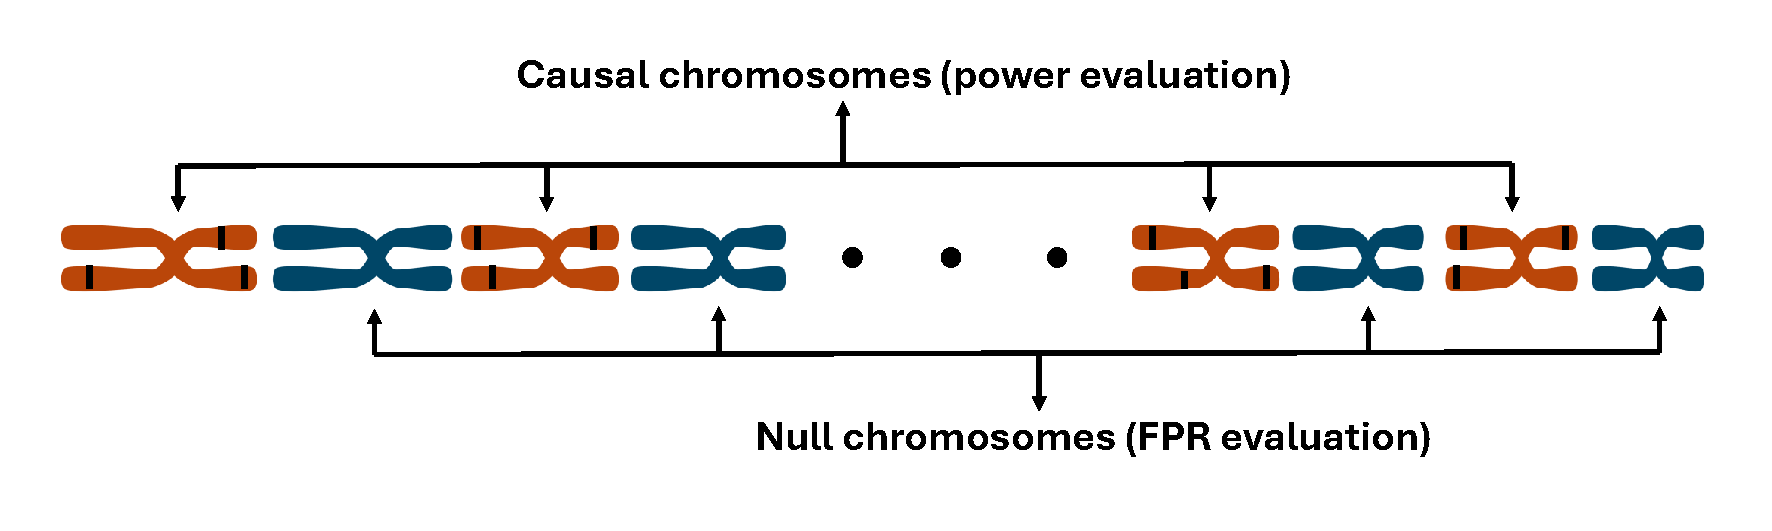
\includegraphics[width=\linewidth]{figures/thesis_qd_sim_design.pdf}
    \caption{\textbf{Phenotype simulation design.} We simulate causal effects using a spike-and-slab, mixture of Gaussian, Laplace or Gaussian distribution only on odd chromosomes, whereas we treat even chromosomes as null controls to test for false positive rate and calibration of test statistics.}
    \label{fig:qd_sim_design}
\end{figure}

In our simulations, we set the variance explained due to population stratification to be $5\%$ of trait variance, whereas sample relatedness explained 10\% of the trait variance in $2^{nd}$ degree relatives and 20\% in $1^{st}$ degree relatives \cite{jiang2019resource}.
%
To simulate a realistic MAF-dependent trait architecture, we set $c_f \propto (2f(1-f))^{\alpha}$, where $f$ is the minor allele frequency and $\alpha = -0.3$ \cite{zeng2018signatures,schoech2019quantification}.
%
For binary traits, we adopted a liability threshold model by synthetizing a quantitative phenotype as in Equation \ref{eq:sim_gen} and setting individuals above/below a given prevalence value as cases/controls.
%
We varied the prevalence in binary traits from 0.3 to 0.001 and the amount of relatedness and population structure based on the following four simulation conditions:
\begin{itemize}
    \item \textbf{Unrelated white British (GB-unrel):}
    %
    We randomly sampled $50{,}000$ individuals from the set of unrelated white British as defined in \cite{bycroft2018uk}.
    %
    This scenario does not include population structure or relatedness.
    %
    \item \textbf{Related white British (GB-rel):}
    %
    We included $25,000$ individuals from the set of individuals in the related white British but not in the unrelated white British subset, along with $25,000$ unrelated white British individuals.
    %
    This resulted in $552$ first degree, $906$ second degree, and $1396$ third degree relative pairs ($3.4 \times$ more relative pairs than randomly sampling from related white British subset). 
    %
    We also considered less and more extreme levels of relatedness, assembling sets of samples by randomly sampling from the related white British subset (referred to as GB-rel-ukb) and including high proportions of first and second degree relatives (referred as GB-rel+ having $7.3 \times$ and $4.8 \times$ more first and second degree pairs than randomly sampling from related white British subset).
    %
    \item \textbf{European structure (EUR):}
    %
    To simulate higher levels of population structure in the dataset, we included $25{,}000$ non-British European samples \cite{bycroft2018uk} along with $25{,}000$ unrelated British samples. This set also comprised $451$ first-degree and $107$ second-degree relative pairs, corresponding to $1.2 \times$ and $0.8 \times$ the amount of first- and second-degree pairs found in the subset of related white British individuals.
    %
    \item \textbf{Pan-ancestry structure (PAS):}
    %
    To simulate population structure comprising multiple ancestry descriptors found in the UK Biobank, we included $7{,}500$ self-reported African samples, $7{,}500$ self-reported South Asian samples, along with $35{,}000$ unrelated British samples, as defiend in \cite{bycroft2018uk}.
    %
    This set comprised $425$ first-degree and $173$ second-degree relative pairs, corresponding to $1.1 \times$ and $1.2 \times$ more first- and second-degree pairs than randomly sampling from the subset of related white British individuals.
    %
    We simulated correlated variant effects across ancestry groups using a multivariate Gaussian, setting the covariance of effects between Africans and other subgroups to $0.4$, and between the European and south-Asian subgroups to $0.7$ \cite{ruan2022improving}.
    %
\end{itemize}
\subsection{False positive rate evaluation}
We verified the calibration of Quickdraws and the other methods by considering varying levels of polygenicity, relatedness, population structure, and the prevalence of binary traits.
%
We measured false positive rates (FPRs), calculated as the proportion of null variants (i.e., variants on even chromosomes) below a chosen p-value threshold. 
%

%
We first tested calibration in analyses involving quantitative traits, considering several simulation settings with population structure and relatedness and varying polygenicity of traits from $1\%$ to $10\%$.
%
In these experiments, linear regression was not robust to the presence of relatedness and population structure, as previously observed \cite{yang2014advantages,loh2015efficient,jiang2019resource}, while all other methods were reasonably calibrated, with a few exceptions (see Figure \ref{fig:qd_sim_fpr_qt}).
%
Like other mixed-model methods, Quickdraws remained calibrated, not showing significant inflation in any of the simulation conditions we considered.
%
Regenie produced significantly inflated test statistics in data sets including high levels of relatedness (t-test $p < 1.5 \times 10^{-4}$, see GB-rel+ in Figure \ref{fig:qd_sim_fpr_qt}), which comprise $1{,}250$ first-degree and $1{,}250$ second-degree relative pairs (corresponding to ${\sim}7.3 \times$ and ${\sim}4.8 \times$ more relatives compared to the white British subset of UK Biobank samples).
%
Finally, we observed higher variance for Quickdraws' FPR estimates in simulations involving non-homogeneous ancestry, due to higher noise in the estimated effective sample size, which relies on a smaller number of unrelated homogeneous individuals.

\begin{figure}[h!]
    \centering
    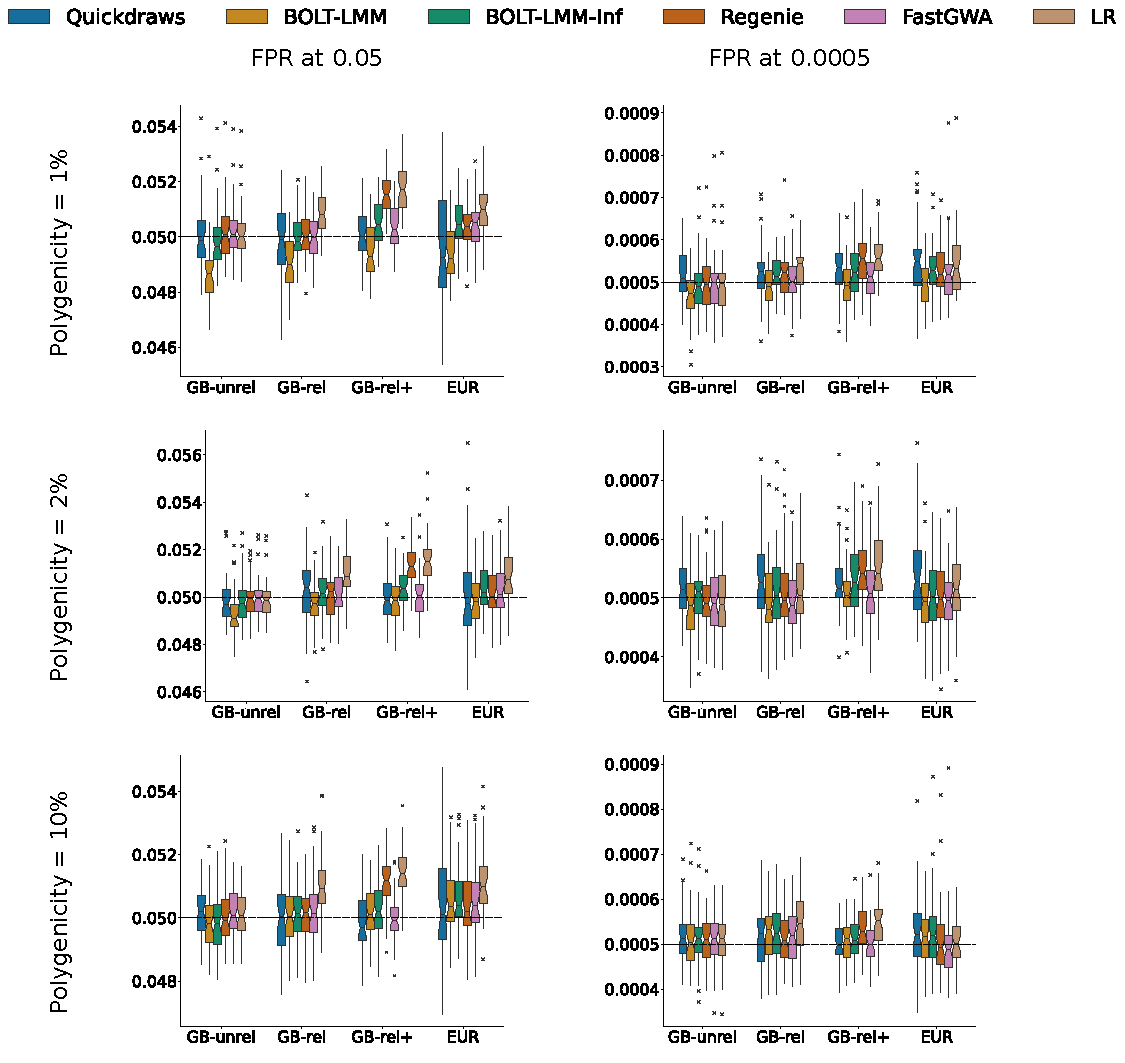
\includegraphics[width=\textwidth]{figures/sim_calibration/qt_fpr.pdf}
    
    \caption{\textbf{Summary of calibration in simulations for quantitative traits.}
    %
    False positive rate (FPR) at a significance threshold of $\alpha \in \{0.05, 0.0005\}$, calculated as the number of variants on even chromosomes with p-value lower than $\alpha$.
    %
    The line inside each box indicates the median value, the central box indicates the interquartile range, whiskers indicate data up to $1.5$ times the IQR, and outliers are shown as separate points.
    %
    A description of the group labels (GB-unrel, GB-rel, GB-rel+, EUR) is provided in section \ref{sec:ch5-sim-design}.
    \label{fig:qd_sim_fpr_qt}
    }
\end{figure}

%
We then assessed statistical robustness in the analysis of binary traits, where we varied the prevalence of the trait from $0.3$ to $0.001$ under varying levels of population structure and relatedness (see figures \ref{fig:qd_sim_fpr_bt1} and \ref{fig:qd_sim_fpr_bt2} for FPR of common and rare variants separately) while fixing the polygenicity of the traits to 2\%. 
%
Binary trait association analysis often violates the normality assumptions made when defining the null distribution of association statistics in linear mixed models, thereby resulting in high FPR, particularly for lower frequency variants or for traits with lower prevalence \cite{zhou2018efficiently}.
%
Consistent with this, BOLT-LMM and BOLT-LMM-Inf, which are not designed for the analysis of low-prevalence binary traits, were inflated across all simulated conditions (t-test $p < 3 \times 10^{-5}$) when the prevalence dropped to or below $0.1$. 
%
Quickdraws produced controlled false positive rates for both common (MAF $> 1\%$) and rare (MAF $< 1\%$) variants in all the simulation settings we considered, which included population structure, relatedness, and low-prevalence binary traits (see figures \ref{fig:qd_sim_fpr_bt1} and \ref{fig:qd_sim_fpr_bt2} respectively).
%
Regenie with Firth logistic regression fallback was inflated for common variants in traits with high prevalence (prevalence $=0.1$ and $0.3$) for several population structure and relatedness settings we considered.
%
When the prevalence of the trait was set to $0.01$ (i.e., $500$ cases out of $50{,}000$ samples) or below, both Quickdraws and Regenie yielded deflated test statistics (t-test $p < 3 \times 10^{-5}$); in scenarios with such a low prevalence, however, all methods we considered lacked sufficient statistical power to detect association ($\chi^2$ at causal variants ${\approx}1$).
%
SAIGE did not converge for up to $28\%$ of the traits when the prevalence dropped to $0.001$, leading to significant deflation (t-test $p < 10^{-15}$). 
%

\begin{figure}[h!]
    \centering
    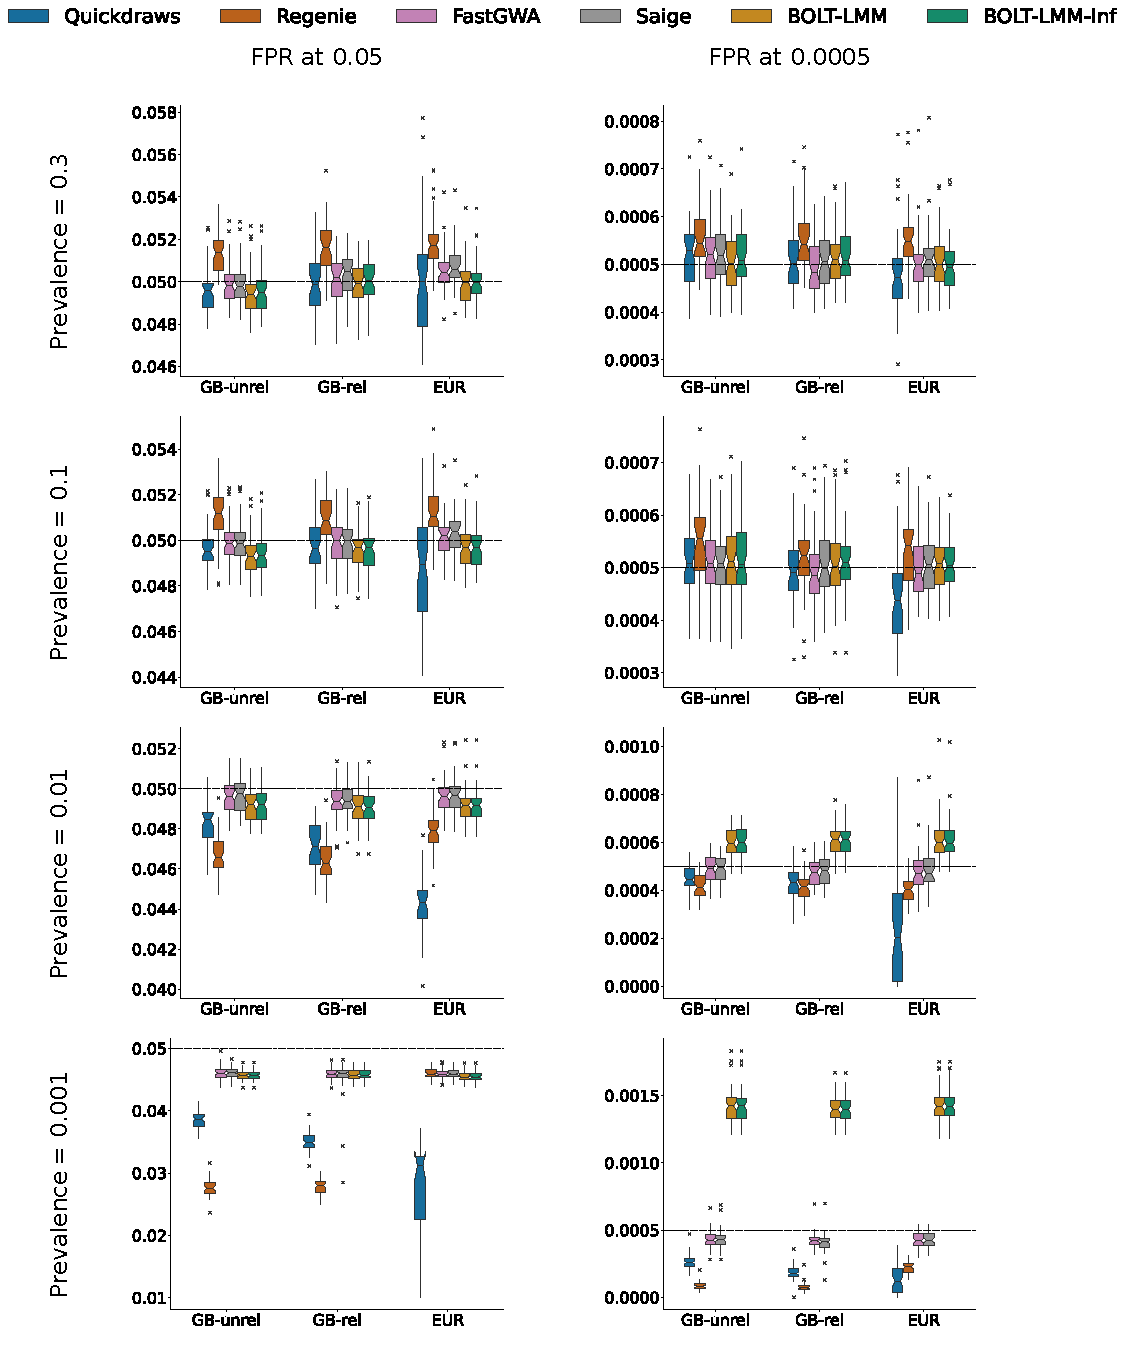
\includegraphics[width=\textwidth]{figures/sim_calibration/bt_fpr_common.pdf}
    \caption{\textbf{Summary of calibration in simulations for binary traits and common variants (MAF $\geq 1\%$).}
    %
    False positive rate (FPR) at a significance threshold of $\alpha \in \{0.05, 0.0005\}$, calculated as the number of variants on even chromosomes with p-value lower than $\alpha$.
    %
    The line inside each box indicates the median value, the central box indicates the interquartile range, whiskers indicate data up to $1.5$ times the IQR, and outliers are shown as separate points.
    %
    A description of the group labels (GB-unrel, GB-rel, EUR) is provided in section \ref{sec:ch5-sim-design}.
    \label{fig:qd_sim_fpr_bt1}
    }
\end{figure}

\begin{figure}[h!]
    \centering
    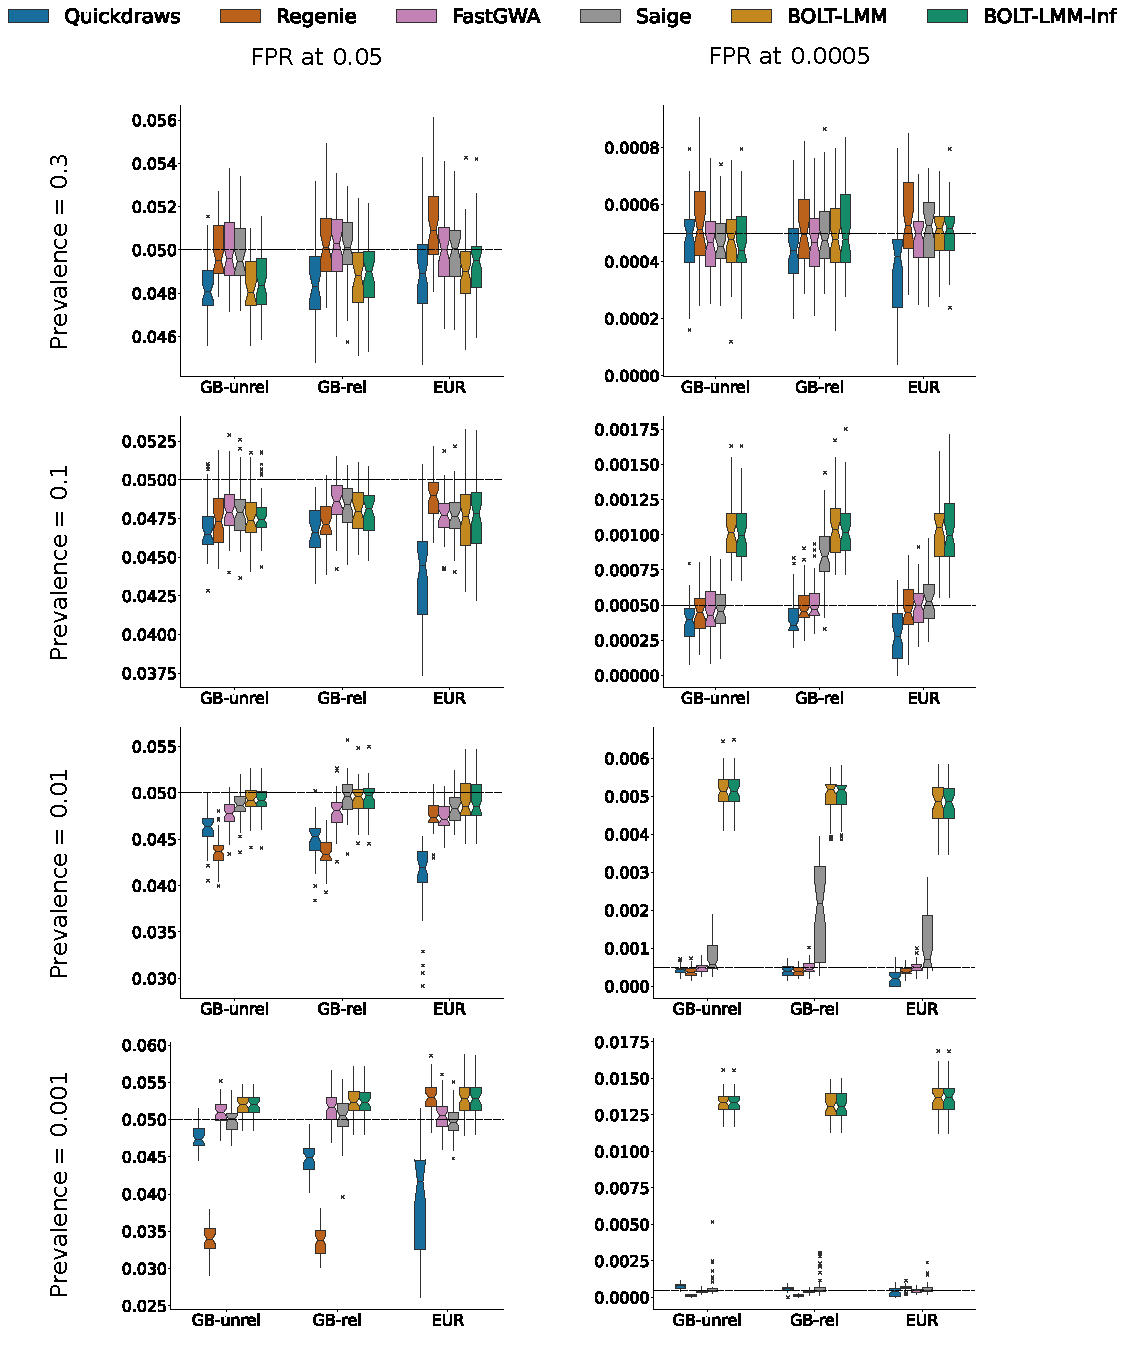
\includegraphics[width=\textwidth]{figures/sim_calibration/bt_fpr_rare.pdf}
    \caption{\textbf{Summary of calibration in simulations for binary traits and rare variants (MAF $< 1\%$).}
    %
    False positive rate (FPR) at a significance threshold of $\alpha \in \{0.05, 0.0005\}$, calculated as the number of variants on even chromosomes with p-value lower than $\alpha$.
    %
    The line inside each box indicates the median value, the central box indicates the interquartile range, whiskers indicate data up to $1.5$ times the IQR, and outliers are shown as separate points.
    %
    A description of the group labels (GB-unrel, GB-rel, EUR) is provided in section \ref{sec:ch5-sim-design}.
    \label{fig:qd_sim_fpr_bt2}
    }
\end{figure}

%
Finally, we verified the calibration of false positive rates in various other simulated conditions, including stronger population structure with up to $30\%$ non-European ancestry (see Figure \ref{fig:sim_calib_pop}), varying levels of relatedness (see Figure \ref{fig:sim_calib_rel}), and genetic architectures involving diverse causal effect size distributions (see Figure \ref{fig:sim_calib_mog}).
%
We also evaluated false positive rates in simulations involving all white British individuals (N $\approx 405k$) and all self-identified European individuals from the UK Biobank (N $\approx 460k$), varying levels of polygenicity in quantitative traits ($1\%$ to $10\%$), and varying levels of prevalence ($0.3$ to $0.001$) in binary traits. We found Quickdraws to yield controlled false positive rates across varying significance thresholds, while fastGWA, Regenie, and BOLT-LMM-Inf led to significant inflation in some cases (see figures \ref{fig:sim_400k}, \ref{fig:sim_460k} and tables \ref{tab:fpr_simulations}, \ref{tab:fgwa_fpr_sims}).
%
This is likely the result of residual population stratification, which is not fully corrected using principal components in these simulated scenarios and, if present, may cause subtle inflation in real-data analyses \cite{haworth2019apparent,sohail2019polygenic,berg2019reduced}.

\begingroup
\renewcommand{\arraystretch}{1.2} % Locally increases the row spacing just for this table

\begin{table}[h!]
\centering
\caption{
\textbf{Summary of calibration in simulations involving (a) $N=405$k white British individuals and (b) $N=460$k European individuals \cite{bycroft2018uk}.} We report the false positive rate (FPR) at a significance threshold of $\alpha \in \{0.05, 0.0005\}$, calculated as the fraction of variants on even chromosomes with p-value lower than $\alpha$.
%
We varied the polygenicity from $1\%$ to $10\%$ in quantitative traits.
%
For binary traits, we changed the prevalence from $0.3$ to $0.001$, fixing the polygenicity to 2\%.
%
Mean FPR refers to the mean across $50$ independent simulated traits, SE refers to standard errors, and p-values are computed for the significance of a deviation from the FPR threshold.
}
\begin{subtable}[h]{\textwidth}
            \centering
\resizebox{\textwidth}{!}{
\begin{tabular}{|c|c|c|c|c|c|}
\hline
\textbf{Simulation Type} & \textbf{FPR Threshold} & \textbf{Polygenicity (QT) / } & \textbf{Mean} & \textbf{SE} & \textbf{T-test} \\ 
 &  & \textbf{Prevalence (BT)} & \textbf{FPR} & \textbf{FPR}  & \textbf{P} \\ 
\hline
\multirow{6}{*}{Quantitative Traits} & \multirow{3}{*}{0.05}  & 1\%   & 0.05034 & 0.00022 & 0.13382 \\ \cline{3-6}
                                     &                        & 2\%   & 0.05040 & 0.00029 & 0.17865 \\ \cline{3-6}
                                     &                        & 10\%  & 0.05036 & 0.00017 & 0.03658 \\ \cline{2-6}
                                     & \multirow{3}{*}{0.0005}& 1\%   & 0.00052 & 0.00001 & 0.06363 \\ \cline{3-6}
                                     &                        & 2\%   & 0.00053 & 0.00002 & 0.04845 \\ \cline{3-6}
                                     &                        & 10\%  & 0.00052 & 0.00001 & 0.04787 \\ \hline
\multirow{8}{*}{Binary Traits}       & \multirow{4}{*}{0.05}  & 0.3   & 0.04923 & 0.00022 & 0.00103 \\ \cline{3-6}
                                     &                        & 0.1   & 0.04986 & 0.00019 & 0.46758 \\ \cline{3-6}
                                     &                        & 0.01  & 0.04940 & 0.00016 & 0.00044 \\ \cline{3-6}
                                     &                        & 0.001 & 0.04648 & 0.00016 & $7.39 \times 10^{-39}$ \\ \cline{2-6}
                                     & \multirow{4}{*}{0.0005}& 0.3   & 0.00048 & 0.00001 & 0.05193 \\ \cline{3-6}
                                     &                        & 0.1   & 0.00051 & 0.00001 & 0.57445 \\ \cline{3-6}
                                     &                        & 0.01  & 0.00046 & 0.00001 & 0.00018 \\ \cline{3-6}
                                     &                        & 0.001 & 0.00042 & 0.00001 & $5.28 \times 10^{-13}$ \\ \hline
\end{tabular}
}
\caption{$N=405$k white British individuals.}
\end{subtable}

\vspace{7mm}

\begin{subtable}[h]{\textwidth}
            \centering
\resizebox{\textwidth}{!}{
\begin{tabular}{|c|c|c|c|c|c|}
\hline
\textbf{Simulation Type} & \textbf{FPR Threshold} & \textbf{Polygenicity (QT) / } & \textbf{Mean} & \textbf{SE} & \textbf{T-test} \\ 
 &  & \textbf{Prevalence (BT)} & \textbf{FPR} & \textbf{FPR}  & \textbf{P} \\ 
\hline
\multirow{6}{*}{Quantitative Traits} & \multirow{3}{*}{0.05}  & 1\%   & 0.05061 & 0.000231 & 0.0098 \\ \cline{3-6}
                                     &                        & 2\%   &0.05019 & 0.00025 & 0.4444 \\ \cline{3-6}
                                     &                        & 10\%  &  0.05037 & 0.00026 & 0.1709 \\ \cline{2-6}
                                     & \multirow{3}{*}{0.0005}& 1\%   & 0.00053 & 0.00001 &  0.0075 \\ \cline{3-6}
                                     &                        & 2\%   & 0.00053 & 0.00001 & 0.01728 \\ \cline{3-6}
                                     &                        & 10\%  &  0.00053 & 0.00001 &  0.0429 \\ \hline
\multirow{8}{*}{Binary Traits}       & \multirow{4}{*}{0.05}  & 0.3   & 0.04983 & 0.00015 & 0.3108 \\ \cline{3-6}
                                     &                        & 0.1   & 0.04997 & 0.00017 & 0.9015 \\ \cline{3-6}
                                     &                        & 0.01  & 0.0437 & 0.00058 & $5.19 \times 10^{-18}$ \\ \cline{3-6}
                                     &                        & 0.001 & 0.03121 & 0.0022 & $3.72 \times 10^{-13} $ \\ \cline{2-6}
                                     & \multirow{4}{*}{0.0005}& 0.3   & 0.00051 & 0.00001 & 0.1391 \\ \cline{3-6}
                                     &                        & 0.1   & 0.00053 & 0.00002 & 0.0436 \\ \cline{3-6}
                                     &                        & 0.01  & 0.00033 & 0.00003 & $4.93 \times 10^{-7}$ \\ \cline{3-6}
                                     &                        & 0.001 & 0.00022 & 0.00003 & $2.47 \times 10^{-15}$ \\ \hline
\end{tabular}
}
\caption{$N=460$k European individuals.}
\end{subtable}

\label{tab:fpr_simulations}
\end{table}

\endgroup % Ends the local redefinition of \arraystretch

\clearpage

\subsection{Statistical power evaluation}
We now focus on evaluating the statistical power of Quickdraws in these simulations.
%
We first tested the performance of Quickdraws in quantitative trait association and compared it with previous association testing methods including BOLT-LMM, Regenie, FastGWA, and an implementation of linear regression provided in Plink \cite{purcell2007plink,chang2015second}.
%
For BOLT-LMM, we also considered a faster implementation that uses infinitesimal priors (BOLT-LMM-Inf), which is more scalable but does not lead to higher association power in less polygenic genetic architectures \cite{loh2015efficient,loh2018mixed}.
%
We measured statistical power by considering the average $\chi^2$ test statistics at simulated causal variants, focusing on the set of unrelated white British samples and varying the number of causal variants in the simulation from $5{,}000$ to $50{,}000$ \cite{zeng2018signatures}.
%
We normalized the average $\chi^2$ test statistics at causal variants by the average $\chi^2$ test statistics at null variants to remove any residual stratification.
%
In these simulations, the modeling of trait polygenicity adopted by Quickdraws led to higher average $\chi^2$ statistics (paired t-test $p < 10^ {-20}$ for polygenicity up to $2\%$) compared to Regenie, FastGWA, BOLT-LMM-Inf, and linear regression (see Figure \ref{fig:sim2_1} and Figure \ref{fig:sim_power_qt} for more simulation conditions).
%
The difference in association power compared to other infinitesimal methods was larger for traits with lower polygenicity (paired t-test $p < 10^{-53}$ for $5{,}000$ causal variants).
%
For instance, when the number of causal variants was reduced to ${5{,}000}$, Quickdraws achieved $\geq 11.46\%$ higher average $\chi^2$ compared to Regenie and BOLT-LMM-Inf (paired t-test $p < 10^{-53}$), resulting in a similarly large gain in effective sample size \cite{yang2011genomic}.
%

%
Next, we applied Quickdraws to the analysis of binary traits, comparing its association power with previous binary trait association methods including SAIGE, Regenie, and FastGWA-GLMM.
%
We simulated phenotypes under a liability threshold model, where cases and controls are defined as individuals who are above or below a chosen liability threshold as described in section \ref{sec:ch5-sim-design}.
%
We fixed the prevalence at $0.3$ and varied the number of causal variants in the simulation from $1{,}250$ to $10{,}000$ \cite{stahl2012bayesian, zeng2018signatures, o2019extreme}.
%
In these experiments, the use of a non-infinitesimal prior in Quickdraws led to higher statistical power compared to SAIGE, Regenie, and FastGWA (paired t-test $p < 10^{-12}$, Figure \ref{fig:sim2_2} and Figure \ref{fig:sim_power_bt} for more simulation conditions).
%
The difference in association power compared to other methods was again larger for traits with lower polygenicity (paired t-test $p < 10^{-43}$ for $1{,}250$ and $2{,}500$ causal variants).
%
For instance, Quickdraws obtained $11.5\%$ and $12.04\%$ higher average $\chi^2$ compared to Regenie and FastGWA on the simulated causal variants for traits with a low polygenicity of $0.25\%$.

\begin{figure}[h!]
    \centering
    % 
\includegraphics[scale=0.335]{figures/sim_power/legend.png}
    \begin{subfigure}{.5\textwidth}
    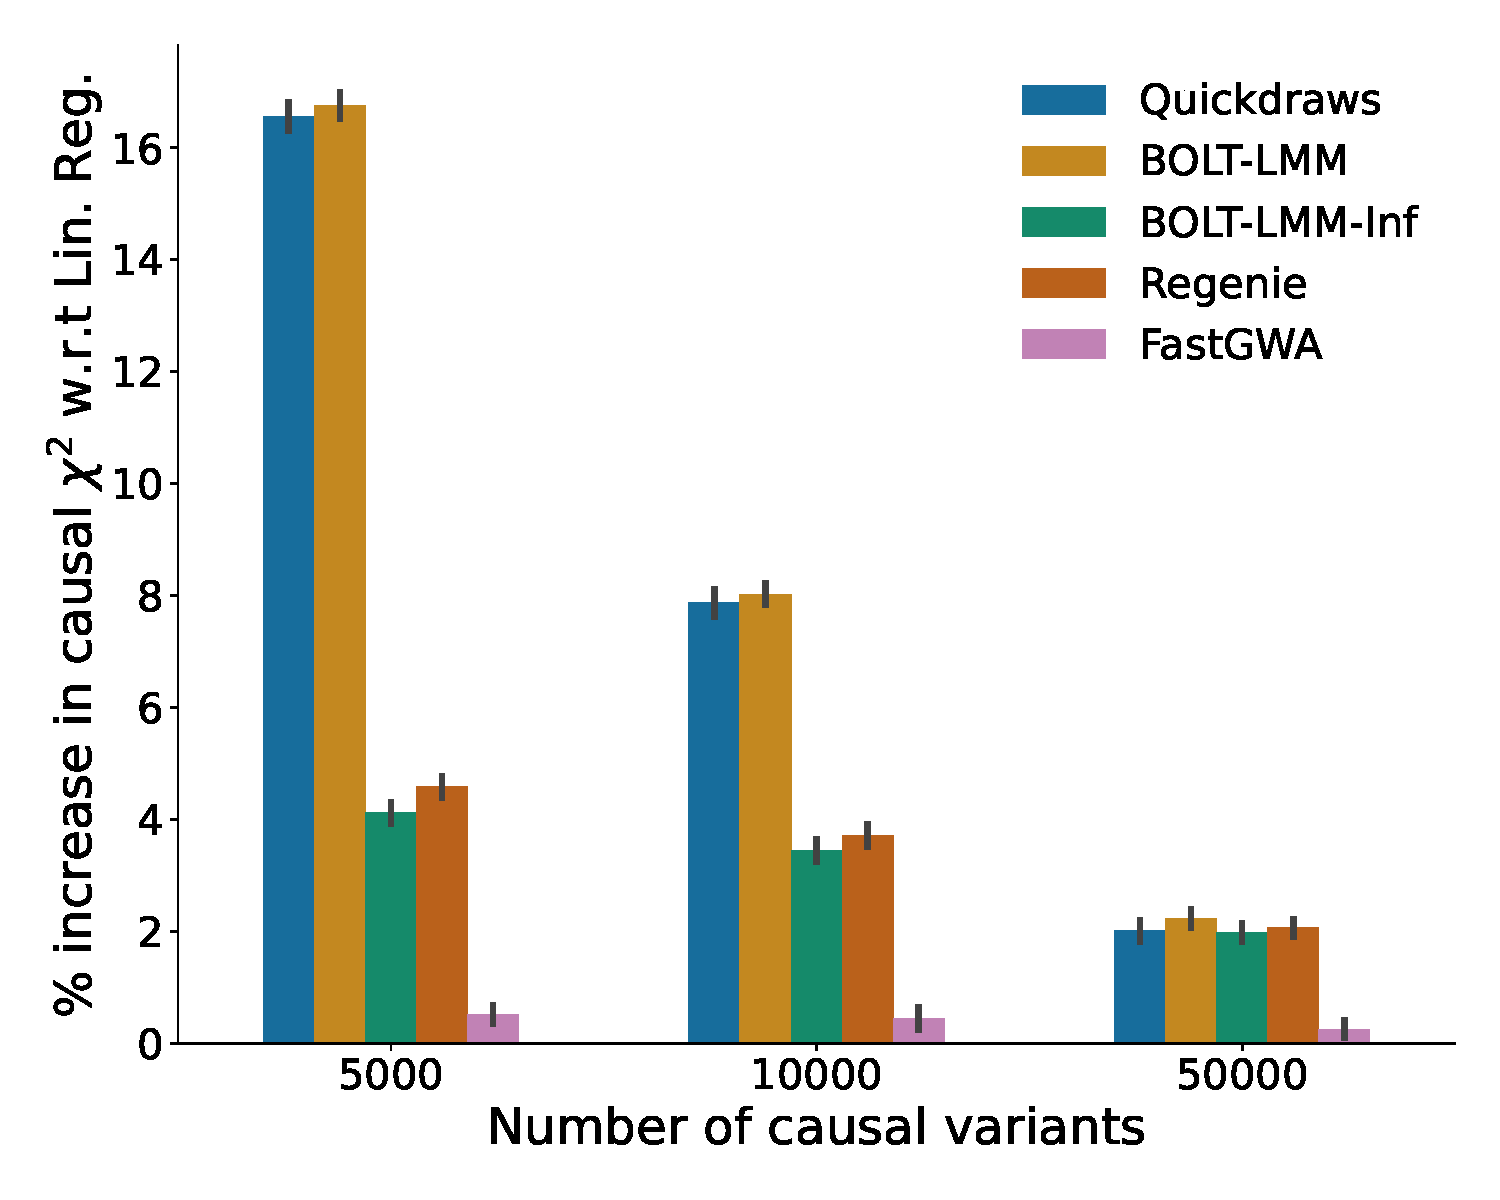
\includegraphics[scale=0.29]{figures/sim_power/paper_result_power_50000.pdf}
    \caption{}
    \label{fig:sim2_1}
    \end{subfigure}%
    \begin{subfigure}{.5\textwidth}
    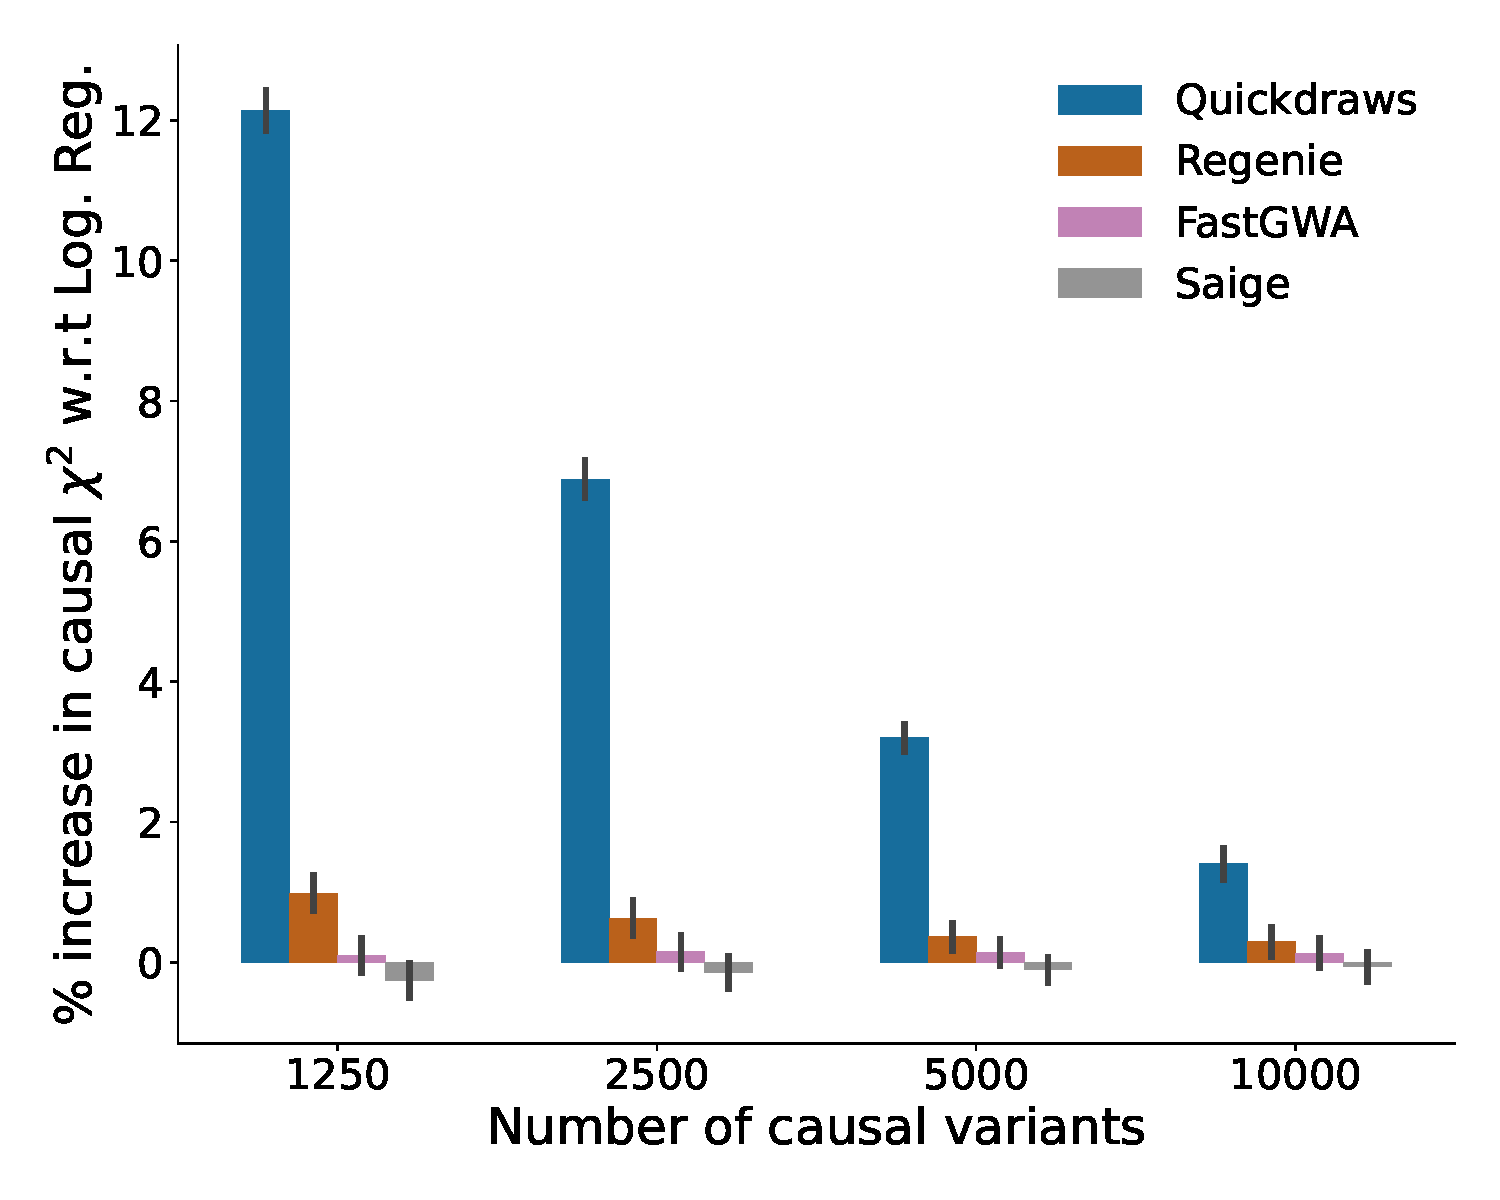
\includegraphics[scale=0.29]{figures/sim_power/paper_result_power_10000.pdf}
    \caption{}
    \label{fig:sim2_2}
    \end{subfigure}
    % \includegraphics[width=\textwidth]{figures/loya_qd_fig1.pdf}
    \caption{\textbf{Statistical power in simulated quantitative and binary traits for unrelated British samples.}
    %
    (a) \% increase in average $\chi^2$ test statistics at causal variants w.r.t.\ linear regression (Lin. Reg.) for quantitative traits, varying the number of simulated causal variants from $5{,}000$ to $50{,}000$ variants.
    %
    (b) \% increase in average $\chi^2$ test-statistics at causal variants w.r.t.\ logistic regression (Log. Reg.) for binary traits, varying the number of simulated causal variants from $1{,}250$ to $10{,}000$ variants.
    %
    Error bars represent the standard error in the percentage improvement, measured using $50$ independent traits.
    %
    The causal $\chi^2$ is normalized by the mean $\chi^2$ at null variants for each trait.
    %
    } 
    \label{fig:sim_power}
\end{figure}

%
Finally, we tested Quickdraws in simulations where causal effects were not assumed to follow a spike-and-slab distribution, where a subset of variants contributes to the phenotype.
%
Instead, we sampled effects from a Gaussian, a mixture of Gaussians, or a Laplace distribution.
%
In the mixture of Gaussians setting, we again observed that Quickdraws and BOLT-LMM yielded higher power compared to other models.
%
In simulations involving fully infinitesimal traits with Laplace and Gaussian effects, Quickdraws and BOLT-LMM produced results similar to other approaches that assume a fully infinitesimal trait architecture (see Figure \ref{fig:sim_power_mog}).
%
We also evaluated power in simulations involving all white British individuals from the UK Biobank ($N \approx 405$k) and all self-identified European individuals from the UK Biobank ($N \approx 460$k).
%
In these settings, we found Quickdraws to provide the highest association power, with higher power than BOLT-LMM when the polygenicity of the trait was low (see figures \ref{fig:sim_400k} and \ref{fig:sim_460k}).
%
%



Overall, these simulations demonstrate that the use of a non-infinitesimal spike-and-slab prior results in higher statistical power to detect association in both quantitative and binary trait simulations.
%
Quickdraws matched or outperformed the power of BOLT-LMM in the analysis of quantitative traits and obtained higher association power than existing GWAS algorithms in binary traits.
%
Quickdraws also yielded controlled FPR in all simulation settings we considered, which included population structure, relatedness, and low-prevalence binary traits.

\begin{figure}[h!]
    \centering
    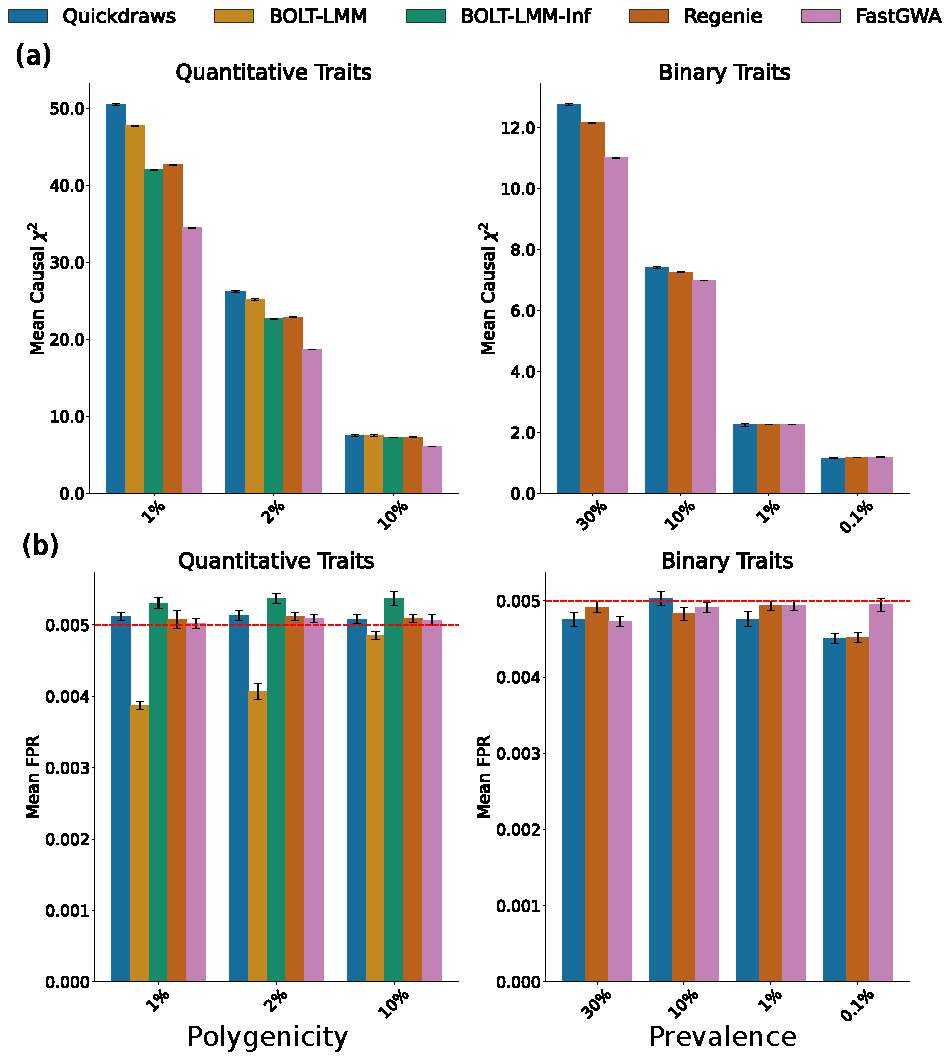
\includegraphics[width=\textwidth]{figures/qd_panel_sim.pdf}
    \caption{\textbf{Power and FPR in N$=405$k simulation.}
    %
    (a) The mean $\chi^2$ at causal variants across different methods and polygenicities for Quantitative traits, and prevalence for binary traits. The $\chi^2$ at causal variants is not normalized by the $\chi^2$ at null variants in this plot.
    %
    (b) The mean false positive rates (FPR) at 0.005 calculated at null variants across different methods and polygenicities for Quantitative traits, and prevalence for binary traits.
    %
    The simulation was performed using the N$=405$k set of white British individuals. The error bars represent 95\% confidence intervals.
    }
    \label{fig:sim_400k}
\end{figure}

\begin{figure}[h]
    \centering
    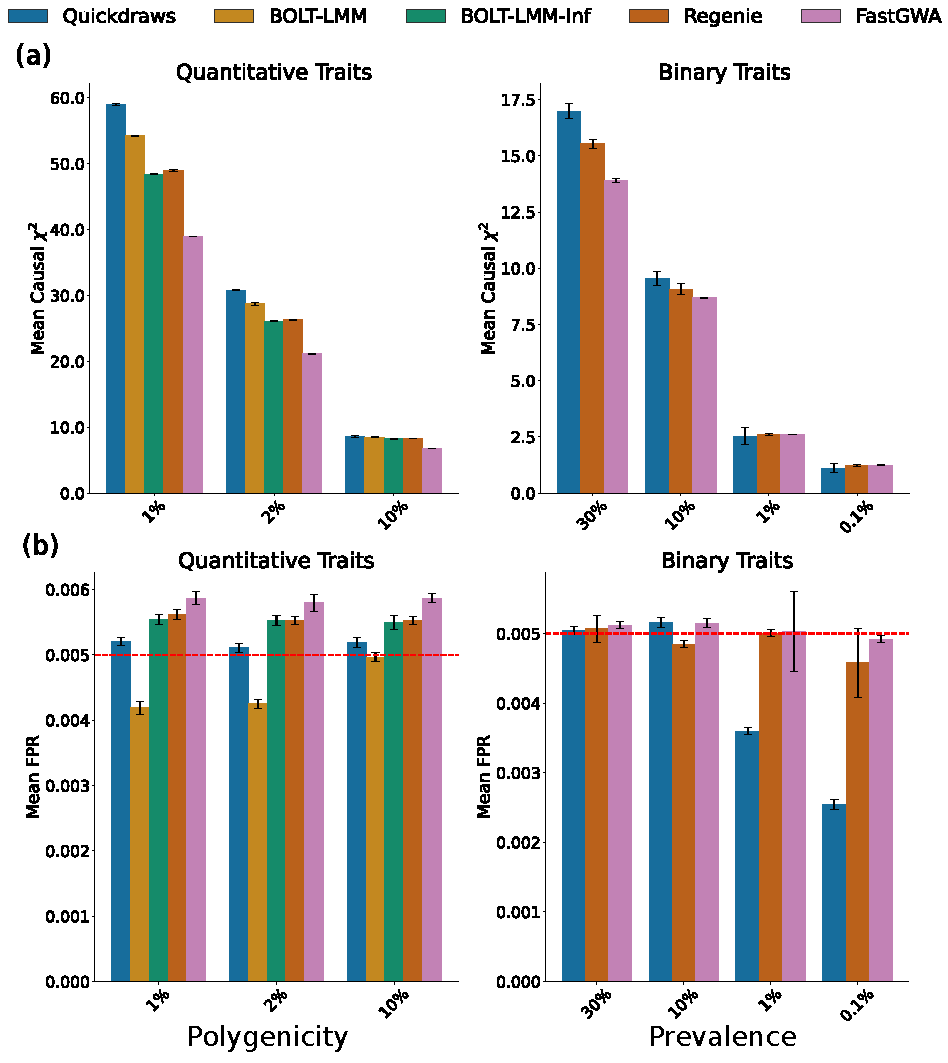
\includegraphics[scale=1]{figures/qd_panel_sim2.pdf}
    \caption{\textbf{Power and FPR in N$=460$k simulation.}
    %
    (a) The mean $\chi^2$ at causal variants across different methods and polygenicities for quantitative traits, and prevalence for binary traits. The $\chi^2$ at causal variants is not normalized by the $\chi^2$ at null variants in this plot.
    %
    (b) The mean false positive rates (FPR) at 0.005 calculated at null variants across different methods and polygenicities for Quantitative traits, and prevalence for binary traits.
    %
    The simulation was performed using the N$=460$k set of UK Biobank self-identified Europeans \cite{bycroft2018uk}. The error bars represent 95\% confidence intervals.
    }
    \label{fig:sim_460k}
\end{figure}

\clearpage

\section{UK Biobank analysis}
\label{sec:ch5-ukb}

We applied Quickdraws to the analysis of $79$ quantitative traits (comprising of blood-related, anthropometric, and other traits) and $50$ self-reported disease traits for ${\sim}405{,}000$ white British individuals from the UK Biobank dataset (see tables \ref{tab:ukb_qt_traits} and \ref{tab:ukb_bt_traits} for the list of traits), which we selected based on their high phenotyping rate and the significance of their estimated heritability as described in section \ref{sec:ch5-data}.
%
We applied standard quality-control filtering steps, retaining $458{,}420$ genotyped markers to be used for model-fitting and ${\sim}13.3$ million imputed variants for association testing.
%
We compared the test statistics we obtained using Quickdraws to those obtained by other association methods, including SAIGE, FastGWA, Regenie, and BOLT-LMM.
%

\subsection{Analysis of false positive rates}
%
We assessed the calibration of the test-statistics in real data by comparing the LD-score regression attenuation ratio estimates \cite{loh2018mixed} obtained using Quickdraws to those obtained using linear regression while restricting to the set of unrelated individuals with homogeneous British ancestry \cite{bycroft2018uk}.
%
Because linear regression is expected to be calibrated in this sample set, similar attenuation ratio estimates for Quickdraws provide evidence for its calibration \cite{loh2018mixed,jiang2019resource}.
%
We performed LD-score regression using the baseline-LD model \cite{gazal2017linkage} and estimated attenuation ratios using test statistics generated using Quickdraws on all ${\sim}13.3$ million testing variants across the set of $79$ quantitative traits.
%
Quickdraws produced attenuation ratios close to those of linear regression on unrelated samples (mean attenuation ratio for Quickdraws $ = 0.0832$, s.e.\ $= 0.008$; mean attenuation ratio for linear regression on unrelated samples $= 0.0892$, s.e.\ $= 0.008$; Figure \ref{fig:real1c}). 
%
Quickdraws also remained calibrated in the analysis of low-prevalence binary traits, where it did not produce signatures of false positive association signals that are present in methods that do not perform adjustments of test statistics such as saddle-point approximation (SPA) \cite{zhou2018efficiently} or approximate Firth logistic regression \cite{mbatchou2021computationally} (see Manhattan plots in figures \ref{fig:qd_man_bin1} and \ref{fig:qd_man_bin2}, additional examples of Manhattan plots for quantitative trait are shown in figures \ref{fig:qd_man_quant1} and  \ref{fig:qd_man_quant2}).
%

\begin{figure}
    \centering
    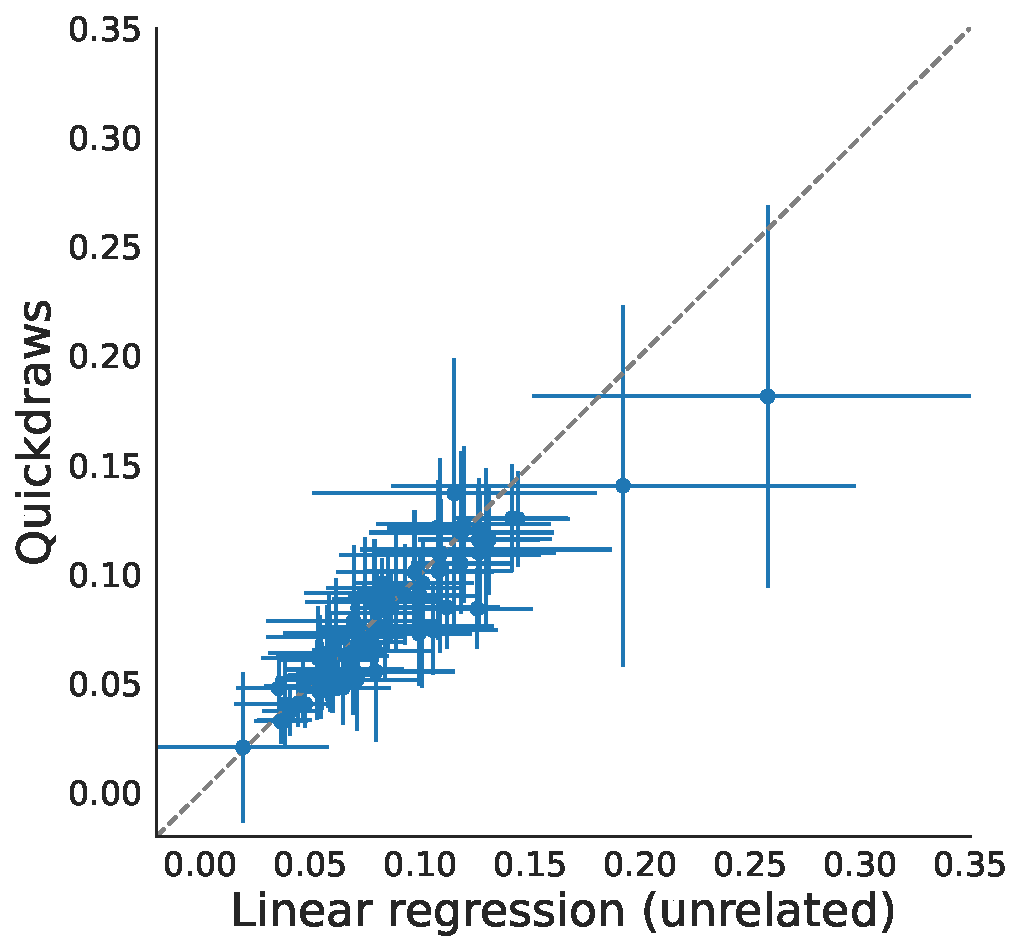
\includegraphics[width=0.65\linewidth]{figures/qd_ukb/attnratio_plot.pdf}
    \caption{\textbf{Calibration in real data analysis.} Attenuation ratio of Quickdraws vs. linear regression in unrelated samples; vertical and horizontal lines represent standard error in the attenuation ratio estimate for each method. }
    \label{fig:real1c}
\end{figure}

%
To further validate signals found using Quickdraws but not found using Regenie, we evaluated the functional annotation of regions where these variants are found.
%
We used the Baseline-LD model annotations \cite{finucane2015partitioning,gazal2017linkage} to assess the distribution of functional annotations for sets of variants associated using different methods.
%
We define the functional enrichment for a set of variants as the proportion of variants being in a particular functional category, divided by the genome-wide fraction of variants assigned to that category.
%
We considered binary and quantitative traits separately and estimated the mean functional enrichment across phenotypes by computing the ratio between the number of variants from a given set that belong to a functional category (numerator) and the total number of variants in the set (denominator).
%
We estimated this ratio by separately summing the numerator and denominator term across all analyzed phenotypes.
%
We estimated standard errors around the enrichment by applying the jackknife method to $50$ equally sized genome blocks.
%
We looked at functional enrichment for various sets of variants, including (1) variants found in Quickdraws but not in Regenie, (2) variants found in both Quickdraws and Regenie.
%
For (2), we matched the $\chi^2$ distribution of the two considered sets, sampling variants detected using Regenie so that they approximately match the empirical $\chi^2$ distribution of the variants detected using Quickdraws.
%
We found similar enrichments compared to variants found using both Regenie and Quickdraws (see figures \ref{fig:functional_qt} and \ref{fig:functional_bt}), suggesting no substantial differences in the functional profile of variants exclusively detected using Quickdraws.
%

\begin{figure}[h!]
    \centering
    \begin{subfigure}{0.5\textwidth}
    \captionsetup{justification=raggedright,singlelinecheck=false}
    \caption*{\textbf{(a)}}
    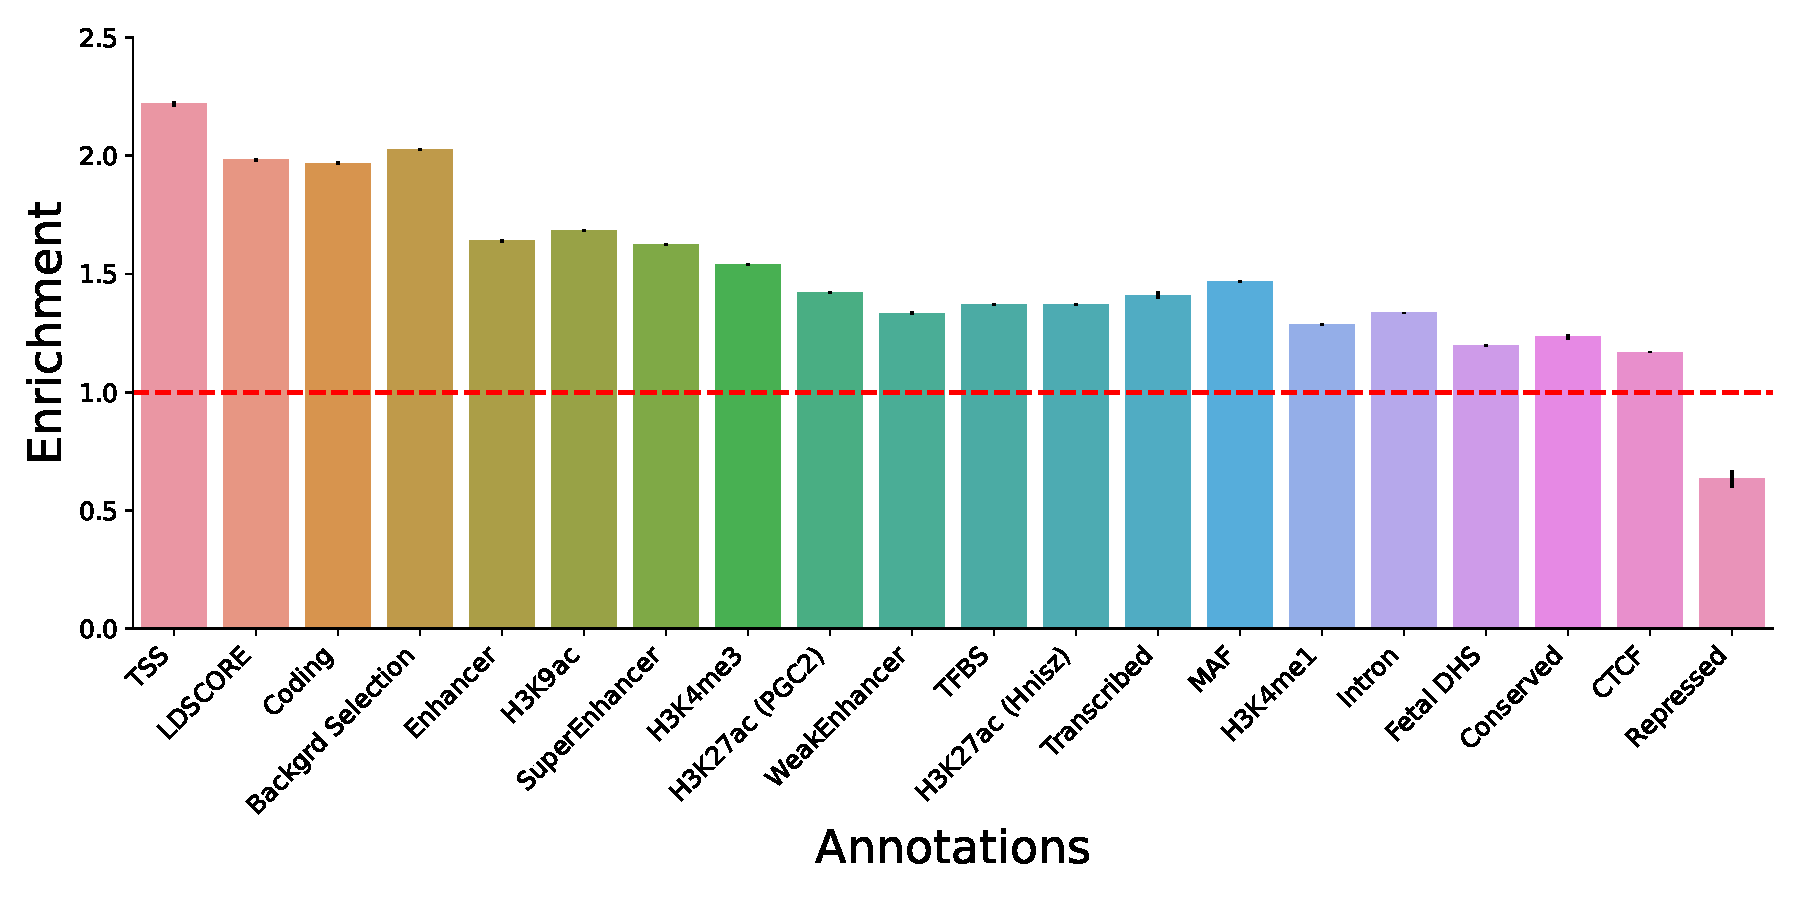
\includegraphics[width=\textwidth]{figures/functional/annotation_both_quant.pdf}
    \end{subfigure}%
    \begin{subfigure}{0.5\textwidth}
    \captionsetup{justification=raggedright,singlelinecheck=false}
    \caption*{\textbf{(b)}}
    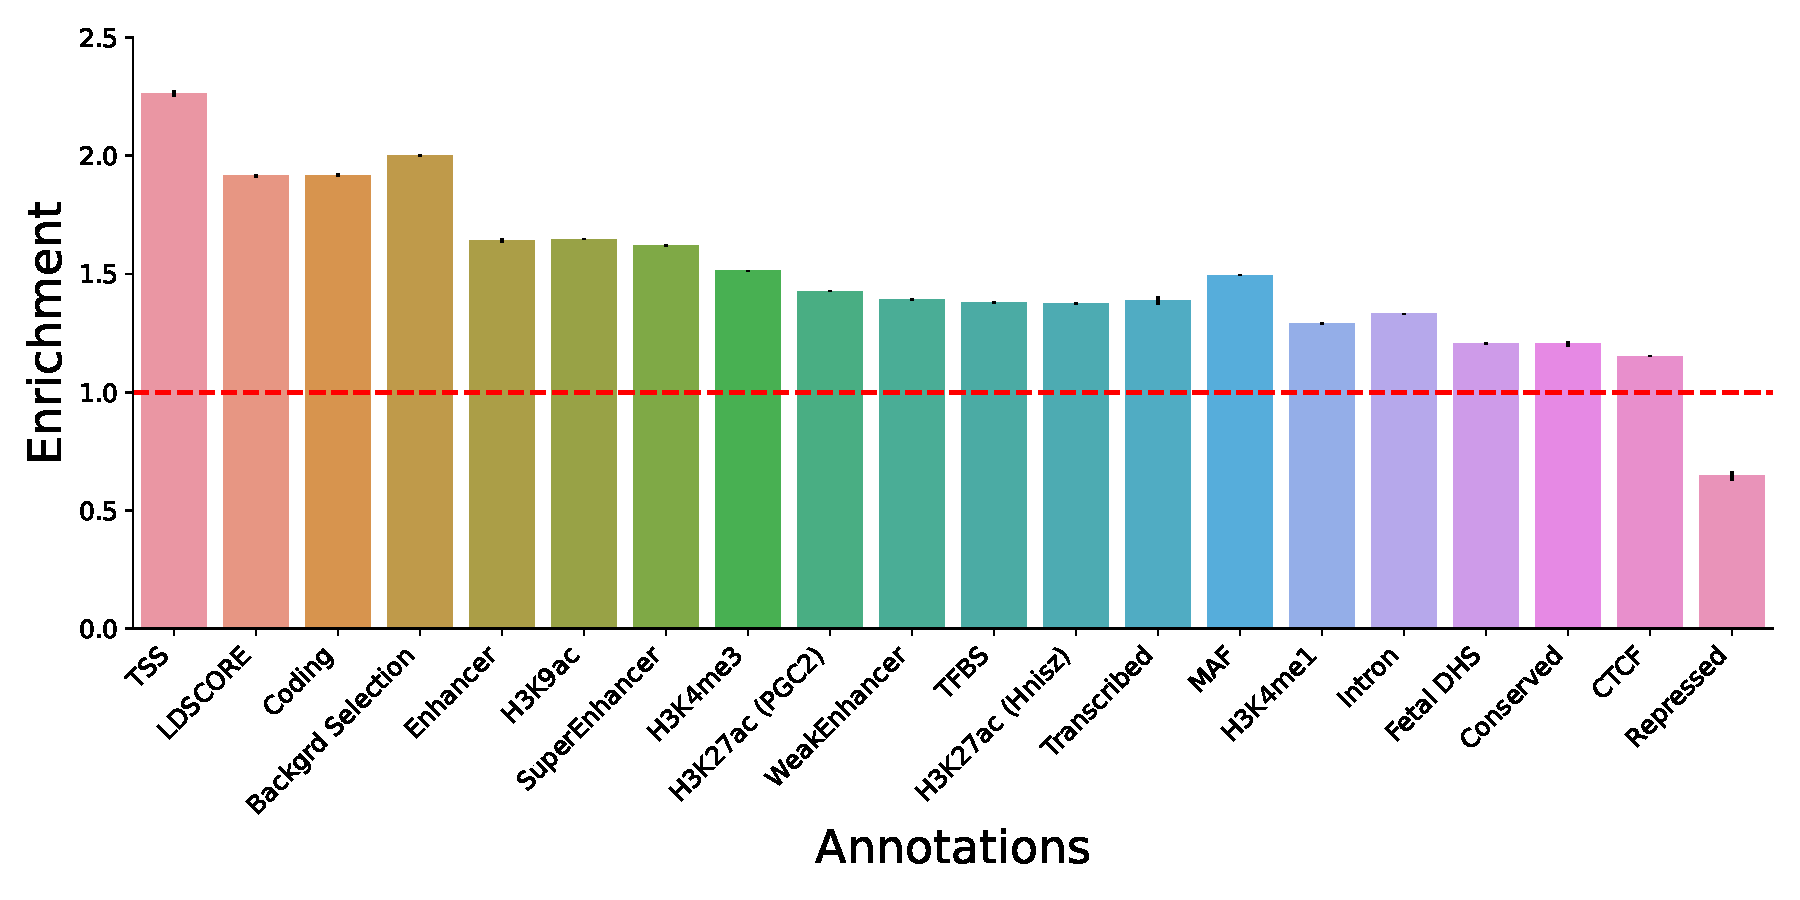
\includegraphics[width=\textwidth]{figures/functional/annotation_onlyqd_quant.pdf}
    \end{subfigure}
    \caption{\textbf{Functional enrichment at associated variants for quantitative traits.}
    %
    Functional enrichment profile of variants associated across $79$ quantitative traits.
    %
    We considered either (a) the set of variants significantly associated ($p \leq 5 \times 10^{-8}$) using both Quickdraws and Regenie, matching the p-value distribution (see Methods), or (b) the set of variants associated using Quickdraws but not Regenie.
    %
    Error bars represent jackknife standard errors; the red dashed line corresponds to no enrichment.
    }
    \label{fig:functional_qt}
\end{figure}

\begin{figure}[h!]
    \centering
    \begin{subfigure}{0.5\textwidth}
    \captionsetup{justification=raggedright,singlelinecheck=false}
    \caption*{\textbf{(a)}}
    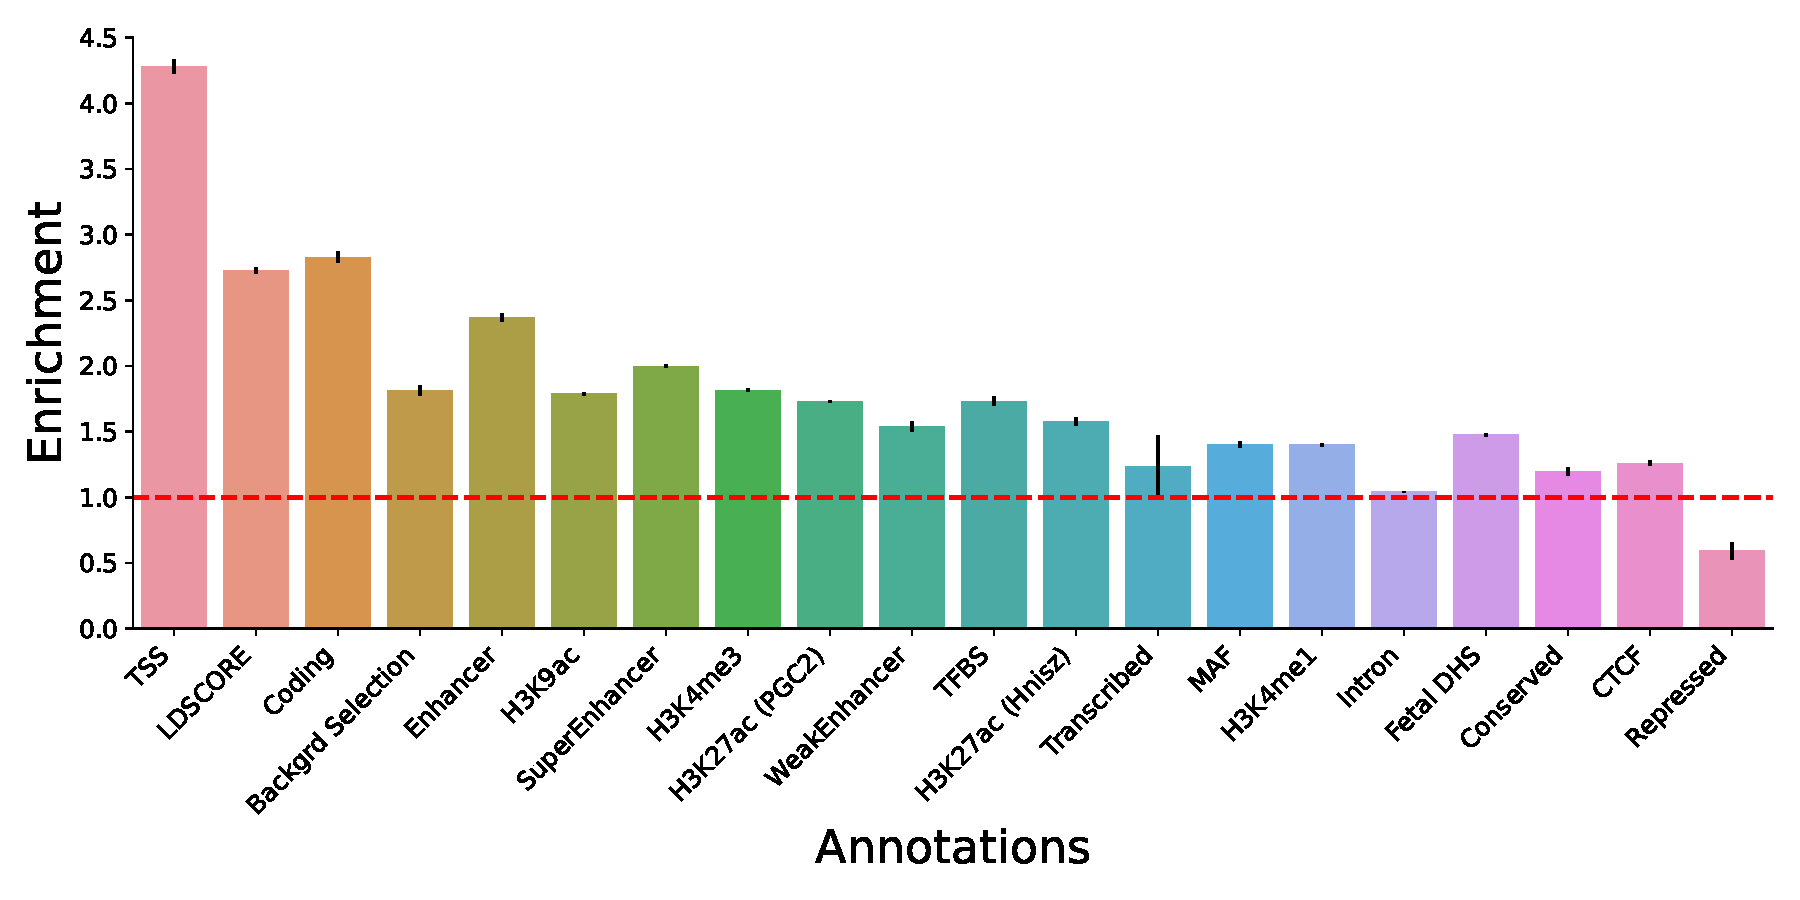
\includegraphics[width=\textwidth]{figures/functional/annotation_both_binary.pdf}
    \end{subfigure}%
    \begin{subfigure}{0.5\textwidth}
    \captionsetup{justification=raggedright,singlelinecheck=false}
    \caption*{\textbf{(b)}}
    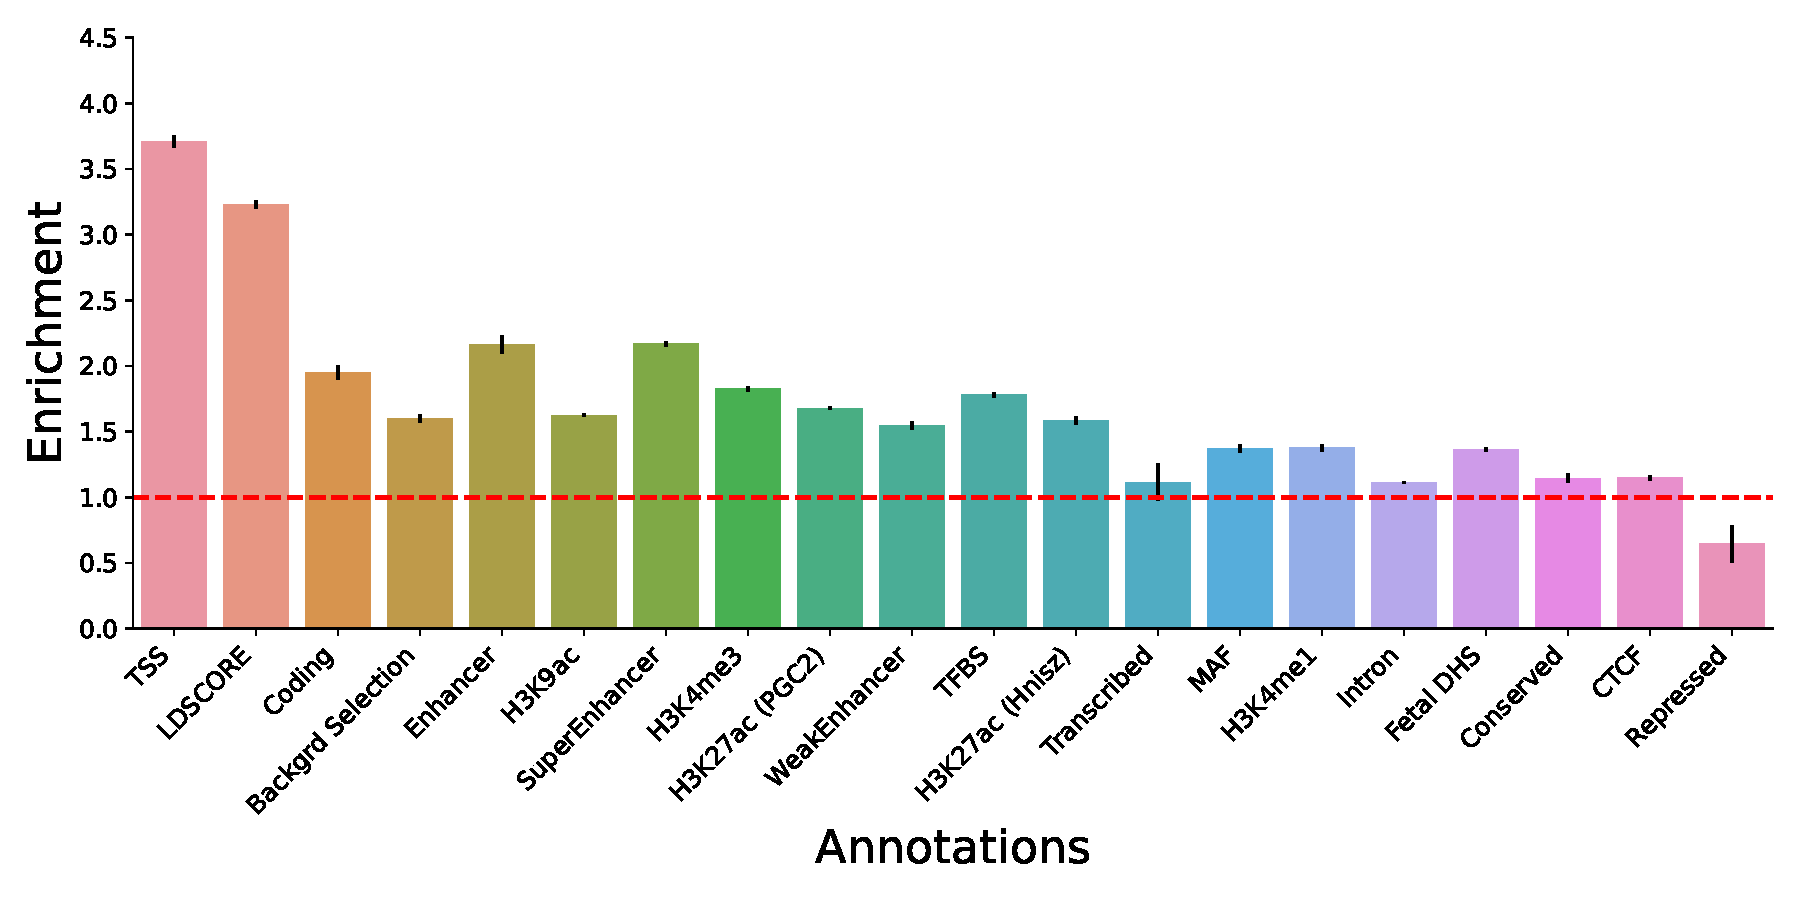
\includegraphics[width=\textwidth]{figures/functional/annotation_onlyqd_binary.pdf}
    \end{subfigure}
    \caption{\textbf{Functional enrichment at associated variants for binary traits.}
    %
    Functional enrichment profile of variants associated across $50$ binary traits.
    %
    We considered either (a) the set of variants significantly associated ($p \leq 5 \times 10^{-8}$) using both Quickdraws and Regenie, matching the p-value distribution (see Methods), or (b) the set of variants associated using Quickdraws but not Regenie.
    %
    Error bars represent jackknife standard errors; the red dashed line corresponds to no enrichment.
    }
    \label{fig:functional_bt}
\end{figure}

\clearpage

\subsection{Number of associations}
We assessed the number of approximately independent associations detected using each method, performing variant clumping with strict filtering criteria (p-value threshold = $5 \times 10^{-9}$, $R^2$ threshold = $0.01$).
%
A summary of these results for Quickdraws, Regenie, and FastGWA, the most scalable methods we tested, is shown in Figure \ref{fig:ukb_indep}a; additional data is reported in tables \ref{tab:loci_qt} and \ref{tab:loci_bt}. 
%
The gains we observed in the number of detected associations were consistent with the increase in power observed in simulations: Quickdraws produced significantly more independent associations compared to Regenie and FastGWA for quantitative and disease traits (binomial test $p < 1.9 \times 10^{-3}$) and a similar number of independent associations compared to BOLT-LMM for quantitative traits (total number of associations, Quickdraws $=26{,}236$, BOLT-LMM $=26{,}368$).
%
In more detail, for quantitative traits, Quickdraws found $4.97\%$ more independent associations compared to Regenie and $22.71\%$ more compared to FastGWA; for disease traits, Quickdraws found on average $3.25\%$ more independent associations compared to Regenie and $7.07\%$ compared to FastGWA.
%
The gain was higher in traits with high heritability or low polygenicity such as mean platelet volume ($8.04\%$ increase over Regenie) and standing height ($26.1\%$ increase over Regenie) \cite{zeng2021widespread}.
%

%
We also analyzed $250$ randomly sampled plasma-protein traits ($N \approx 43$k, see Methods), which have a less polygenic architecture than the other quantitative traits we considered \cite{sun2023plasma}.
%
In these analyses, Quickdraws found significantly more independent association signals compared to Regenie (5.54\% more loci, $p = 6.6 \times 10^{-3}$, see Figure \ref{fig:ukb_indep}b).
%
Finally, we estimated the effective sample size, calculated as the average $\chi^2 - 1$ association statistic at variants that were found to be significantly associated (p $<5 \times 10^{-8}$) using linear regression model applied to unrelated homogeneous subset of the data \cite{yang2011genomic}.
%
We found the effective sample size estimated for Quickdraws to be $14.7\%$ higher ($p = 7.6 \times 10^{-4}$) than FastGWA and $3.4\%$ ($p = 0.197$) higher than Regenie, while being similar to that of BOLT-LMM ($p = 0.46$) when applied to quantitative traits (see Figure \ref{fig:ukb_indep}c-d).
%

\begin{figure}[h!]
    \centering
    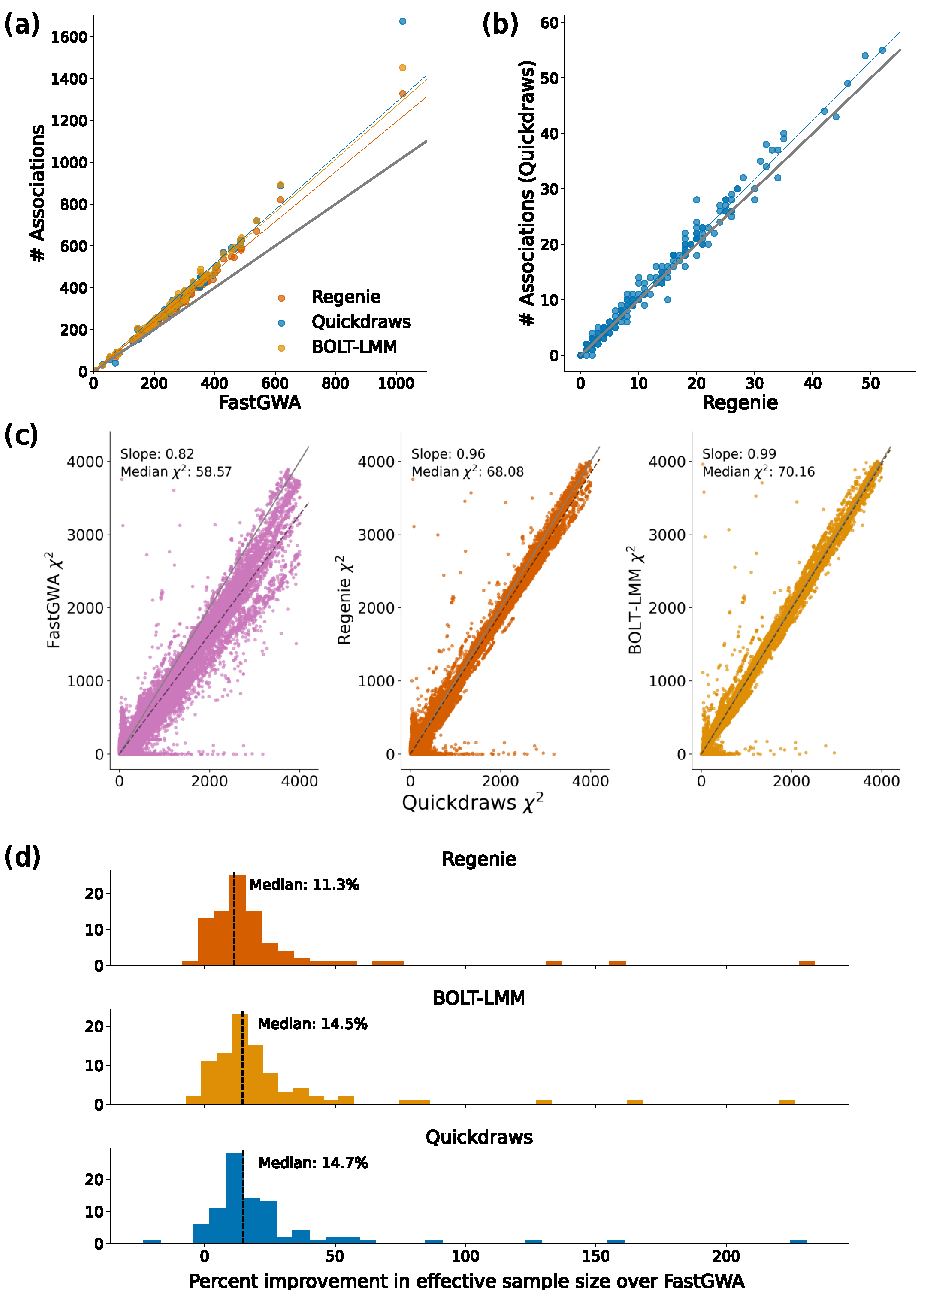
\includegraphics[scale=0.7]{figures/qd_panel_loci.pdf}
    \caption{\textbf{Approximately independent loci and effective sample size in UK Biobank analysis.} (a) Number of approximately independent loci after plink clumping in FastGWA (x-axis) vs. Regenie, BOLT-LMM, and Quickdraws for 79 quantitative traits. (b) Number of approximately independent loci after plink clumping in Regenie (x-axis) vs. Quickdraws for 250 randomly sampled plasma protein traits. (c) The $\chi^2$ for 79 quantitative traits and N$=405$k UK Biobank set conditioned on genome-wide significance ($p < 5 \times 10^{-8}$) in linear regression run on unrelated subset of the data (N$=337$k). Median $\chi^2$: FastGWA $= 58.57$, Regenie $= 68.08$, BOLT-LMM $= 70.16$ Quickdraws $= 70.64$. (d) Histogram of the effective-sample size increase compared to FastGWA for 79 quantitative traits, measured as the mean $\chi^2$ minus 1 at genome-wide significant variants inferred though linear regression run on unrelated subset of the data (N$=337$k). For (a-c) The gray line represents the y=x line and the dashed lines represent a linear regression fit for each method, for (d) the dashed line represents the median improvement in effective sample-size across traits.}
    \label{fig:ukb_indep}
\end{figure}

\clearpage

\subsection{Replication analysis with Biobank Japan, Finngen and other large-scale GWAS}

To validate the additional associations detected using Quickdraws, we performed a replication analysis using GWAS summary statistics from the Biobank Japan data set \cite{nagai2017overview}, which used BOLT-LMM-Inf and SAIGE to detect associations, FinnGen, \cite{kurki2023finngen} which used Regenie, and other trait-specific large-scale studies \cite{jostins2012host, diabetes2012large, dubois2010multiple, nagel2018meta, de2017genome}
%
We assessed the number of variants detected using different GWAS methods that can be replicated in the Biobank Japan, FinnGen and other large-scale studies, using downloaded summary association statistics.
%
We considered $30$ quantitative traits and $13$ self-reported disease traits from Biobank Japan, as well as $21$ self-reported disease traits from FinnGen for which equivalent definitions were available in both our analyses and the replication data set, and for which at least one significant association was detected in both studies.
%
We also considered 5 disease traits (Crohn's disease \cite{jostins2012host}, Type 2 Diabetes \cite{diabetes2012large}, Celiac disease \cite{dubois2010multiple}, Depression \cite{nagel2018meta} and Ulcerative Colitis \cite{de2017genome}) that have publicly available summary statistics calculated on higher number of cases than in the UK Biobank.
%
We considered variants with MAF $\geq 0.1\%$, INFO score $\geq 0.8$, and appearing in both UK Biobank and the replicating dataset, leading to ${\sim}5.89$ million variants available for Biobank Japan replication, and ${\sim}10.89$ million variants available for FinnGen replication.
%

%
We separately considered the replication of associated variants and loci.
%
For the replication of individual variants, we assessed the number (and proportion) of variants detected ($P_{dis} \leq 5 \times 10^{-9}$) in the UK Biobank that are also significant in Biobank Japan, using multiple replication thresholds, $P_{rep} \leq 5 \times 10^{-2}$, $P_{rep} \leq 5 \times 10^{-4}$, and $P_{rep} \leq 5 \times 10^{-6}$.
%
Where, $P_{dis}$ and $P_{rep}$ are the significance thresholds for discovery and replication.
%
For the replication of loci, we followed a procedure similar to that adopted in \cite{huang2022transferability}, defining a credible set for a locus to contain a lead (or sentinel) associated variant together with additional proxy variants found within a $50$ kb window from the lead variant and with association significance $P \leq 100 \times P_{sentinel}$.
%
We defined a locus as replicated if any variant in the credible set was also found to be associated (at $P \leq 5 \times 10^{-2}$) with the same direction of effect in the replication cohort.
%
First, we calculated the average replication rate for each trait using all GWAS methods (FastGWA, Regenie, and Quickdraws) with a discovery threshold of $5 \times 10^{-9}$.
%
Then, we adjusted the discovery threshold for each method, varying it from $2 \times 10^{-9}$ to $8 \times 10^{-9}$, to achieve the same replication rate for each method.


Across the $53$ quantitative and disease traits available in Biobank Japan and Finngen (which comprise $40$ independent traits based on squared phenotypic correlation $\leq 0.1$), Quickdraws yielded a significantly higher number of replicated loci compared to Regenie (binomial test $p=0.014$) and FastGWA (binomial test $p=7 \times 10^{-4}$).
%
For the set of $30$ quantitative traits present in both studies, we observed a $2.5\%$ and $15.72\%$ increase over Regenie and FastGWA, respectively, and a similar number of replicated loci compared to BOLT-LMM (total number of replicated loci, Quickdraws $=37{,}210$, BOLT-LMM $=37{,}072$).
%
For the smaller set of $23$ overlapping disease traits we analyzed, Quickdraws obtained $1.07\%$ and $3.38\%$ more replicated loci compared to Regenie and FastGWA, respectively.
%
We observed a similar increase in the number of replicated loci for $5$ disease traits where we had access to meta-analyzed summary statistics from large-scale studies (see Table \ref{tab:repl5}).
%
We verified that this increase in the number of replicated loci did not correspond to a decrease in replication rates across these methods (see Table \ref{tab:repl1} and Figure \ref{fig:ukb_repl}d-e).
%
A Venn diagram depicting the relationships between sets of variants replicated using different methods is shown in Figure \ref{fig:ukb_repl}b-c.
%
Note that these results may be affected by the choice of GWAS method used in the replication cohort.

\begin{figure}[h!]
    \centering
    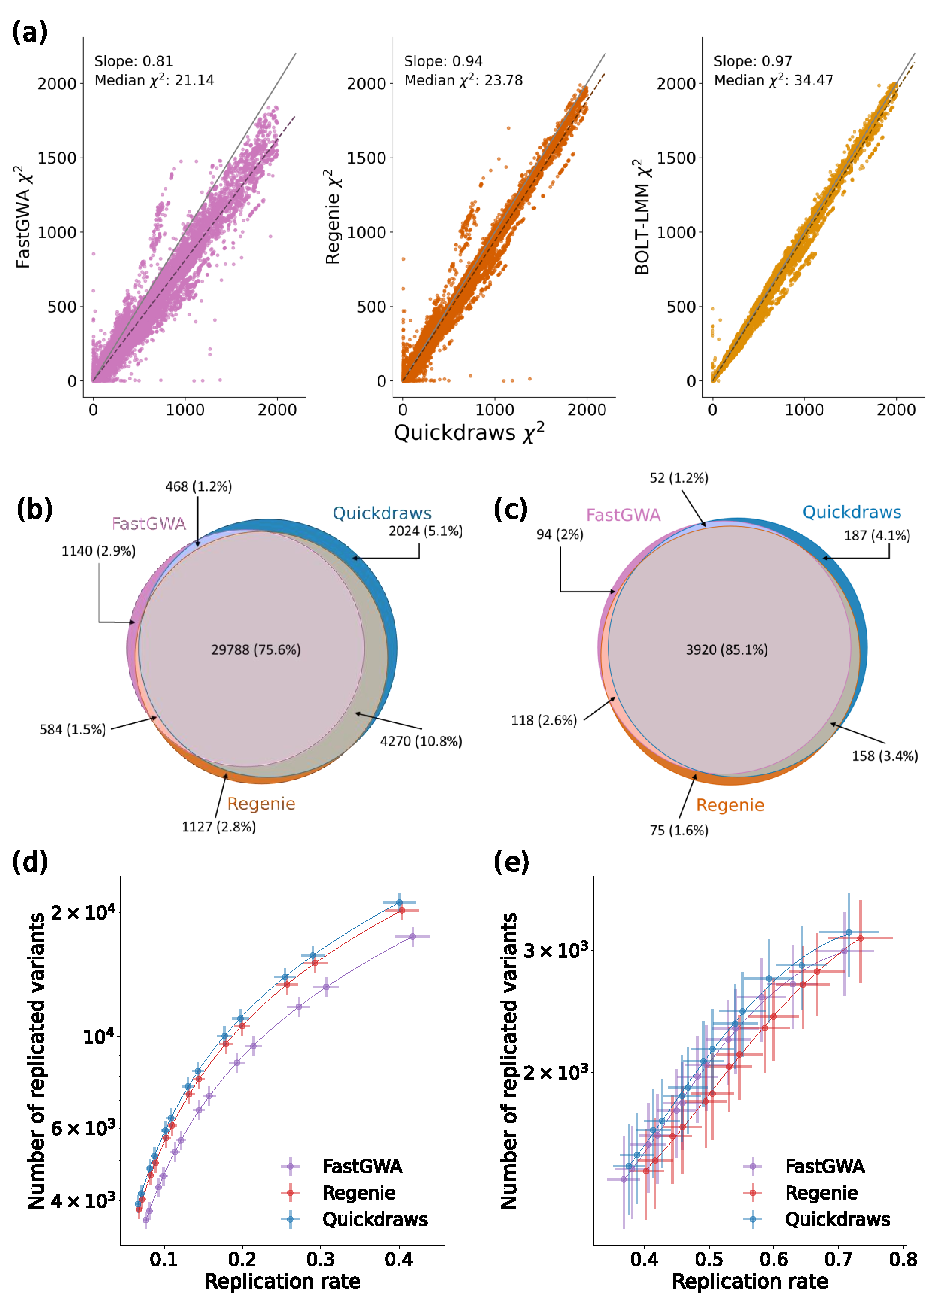
\includegraphics[scale=0.7]{figures/qd_panel_replication.pdf}
    \caption{\textbf{Replication analysis in Biobank Japan and Finngen.} (a) The $\chi^2$ in UK Biobank conditioned on genome-wide significance ($p < 5 \times 10^{-8}$) in replicating biobank across GWAS methods. The variants are aggregated across traits, quantitative and binary traits for Regenie and FastGWA, and only quantitative traits for BOLT-LMM. The gray line represents the y=x line, and the dashed line the linear regression fit without intercept. Median $\chi^2$ for quantitative traits: FastGWA $= 28.36$, Regenie $= 33.44$, BOLT-LMM $= 34.47$ Quickdraws $= 36.32$; binary traits: FastGWA $= 14.08$, Regenie $= 14.34$, Quickdraws $= 14.51$. (b-c) Replication venn diagram for (b) 30 overlapping quantitative traits in Biobank Japan and (b) 23 overlapping binary traits in Biobank Japan and Finngen. (d-e) Number of replicated variants vs replication rate for (d) quantitative and (e) binary traits. The discovery threshold was fixed to $5 \times 10^{-9}$ and the replication threshold was varied from $5 \times 10^{-2}$ to $5 \times 10^{-8}$. The error bars represent standard errors calculated using block jack-knife across chromosomes. The dashed line represents a cubic spline fit to the datapoints.}
    \label{fig:ukb_repl}
\end{figure}



\clearpage

\subsection{Predictive power in out-of-sample data}

To verify that these power gains are due to the modeling of non-infinitesimal trait architectures, we measured the accuracy of the polygenic predictions computed by Quickdraws, BOLT-LMM, and BOLT-LMM-Inf during the model fitting step \cite{loh2015efficient,loh2018mixed}.
%
To this end, we used predictors from step 1 trained on the ${\sim}405{,}000$ white British subset to perform trait prediction for the remaining individuals.
%
Across $79$ quantitative traits, Quickdraws and BOLT-LMM obtained a mean correlation between true and predicted trait in the held-out European samples of $0.307$ (s.e $= 0.0061$) and $0.313$ (s.e $= 0.0061$), respectively, whereas BOLT-LMM-Inf yielded a lower correlation of $0.271$ (s.e $= 0.0061$) (see Figure \ref{fig:ukb_pgs}a).
%
Similar improvements due to the modeling of non-infinitesimal trait architectures have also been observed in the context of polygenic prediction \cite{vilhjalmsson2015modeling,loh2015efficient,loh2018mixed,lloyd2019improved,prive2020ldpred2}.
%

\subsubsection{Comparison with PGS methods}

We also compared the predictions from step 1 of Quickdraws with polygenic scores (PGS) built using recent methods \cite{euesden2015prsice, ge2019polygenic}.
%
To this end, we constructed PGS for all the $79$ quantitative traits analyzed, using either pruning and thresholding (P+T) as implemented in PRSice \cite{euesden2015prsice} or the PRS-CS method \cite{ge2019polygenic}.
%
We used summary statistics generated using various methods on the set of ${\sim}13.3$ million imputed variants to generate PGS for held-out individuals from European, South Asian, East Asian, and African subgroups of the UK Biobank.
%
We report the mean predictive $R^2$ and the $95\%$ confidence interval across all analyzed traits, obtained using a meta-analysis of Fisher-transformed estimated correlation coefficients.

%
We found Quickdraws' step 1 predictors to be significantly more accurate (paired t-test  $p < 5.6 \times 10^{-6}$ compared to PRS-CS and P+T) than summary-statistics derived PGS methods in the European held-out set, while achieving similar accuracy in other groups (see Figure \ref{fig:ukb_pgs}b).
%
In addition, we compared the accuracy of PGS estimates built based on summary association statistics obtained using different association algorithms.
%
Consistent with a recent analysis that did not observe higher accuracy for PGS built from summary statistics derived from non-infinitesimal modeling \cite{weissbrod2022leveraging}, we did not observe significant differences between using Quickdraws, BOLT-LMM, or Regenie, but found PGS built using summary statistics from FastGWA to be significantly less predictive (paired t-test $p < 2.2 \times 10^{-4}$ for both PRS-CS and P+T in European and South-Asian held-out samples, see Figure \ref{fig:ukb_pgs}c-d).
%

\begin{figure}[h!]
    \centering
    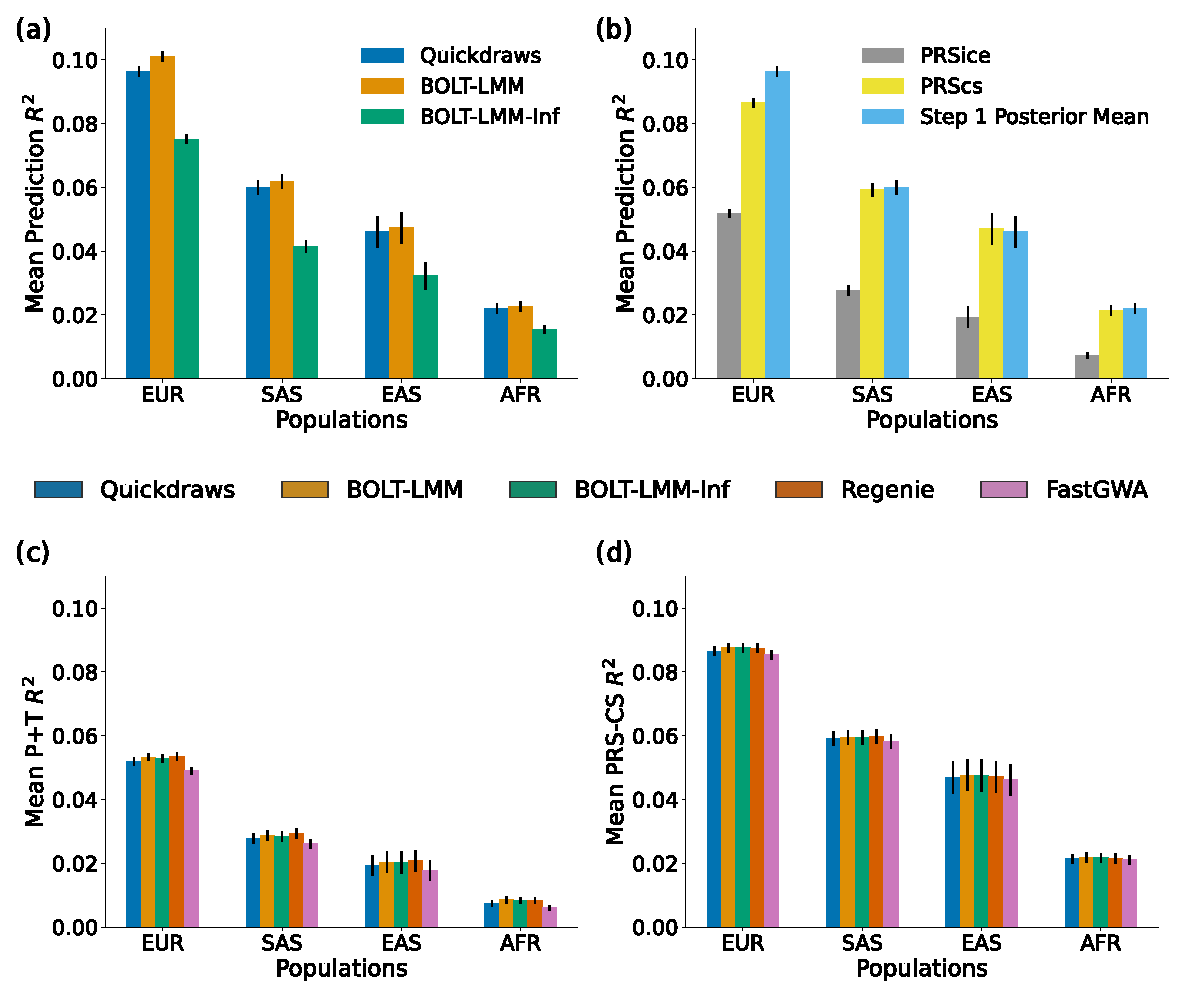
\includegraphics[width=\textwidth]{figures/qd_panel_pgs.pdf}
    \caption{\textbf{Phenotype prediction analyses in the UK Biobank.} (a) Held-out mean phenotype prediction $R^2$ comparing step 1 posterior estimates from Quickdraws, BOLT-LMM and BOLT-LMM-Inf. (b) Comparing Quickdraws' step 1 posterior estimates with PGS calculated using Quickdraws' association statistics and P+T (pruning and thresholding as implemented in PRSice) or PRS-CS. (c-d) Comparing predictive power for PGS calculated using association statistics from different GWAS methods and different PGS methods, (c) P+T as implemented in PRSice and (d) PRS-CS. All analyses was performed on $27{,}683$ held-out non-British Europeans, $9{,}044$ self-identified south Asians, $1{,}457$ self identified east Asians and $7{,}204$ self identified African of African American samples. Results are aggregated across the $79$ quantittaive traits we analyzed, and the error bars represent 95\% confidence interval of the mean prediction $R^2$ for each method in each population subgroup.}
    \label{fig:ukb_pgs}
\end{figure}

\subsubsection{Comparison with PGS adjusted GWAS}

This analysis was performed by Dr. Georgios Kalantzis, who is one of the co-authors on the paper.
%
We briefly experimented with using polygenic scores as covariates when performing association, a strategy recently shown to effectively increase association power \cite{bennett2021controlling, campos2023boosting, jurgens2023adjusting}.
%
For this analysis, we focus on chromosomes $1$ to $5$, using up to $405{,}088$ samples from the white British subgroup, and analyzing all $79$ quantitative traits.
%
We first generate leave-one-chromosome-out (LOCO) polygenic scores, as described in \cite{bennett2021controlling}, using PRS-CS and summary statistics computed with FastGWA or Regenie.
%
We then used FastGWA and Regenie to test for association again, this time including the LOCO PGS corresponding to the chromosome of the variant being tested as a covariate, during both the model-fitting and association steps.

%
Consistent with recent results \cite{bennett2021controlling, jurgens2023adjusting}, we found that this approach increased the effective sample size for FastGWA, which relies on approximate sparse GRMs.
%
While showing no improvement in power for Regenie, which already uses genome-wide regression to account for polygenic effects.
%
The effective sample size and total number of genome-wide significant hits, however, remained lower than that achieved using Quickdraws or BOLT-LMM (see Figure \ref{fig:prs_adjustment}).
%

\begin{figure}[h]
    \centering
    % \includegraphics[scale=0.45]{figures/fig.prs_adjustment.summary.mean_loci.chr_jknf.eps}
    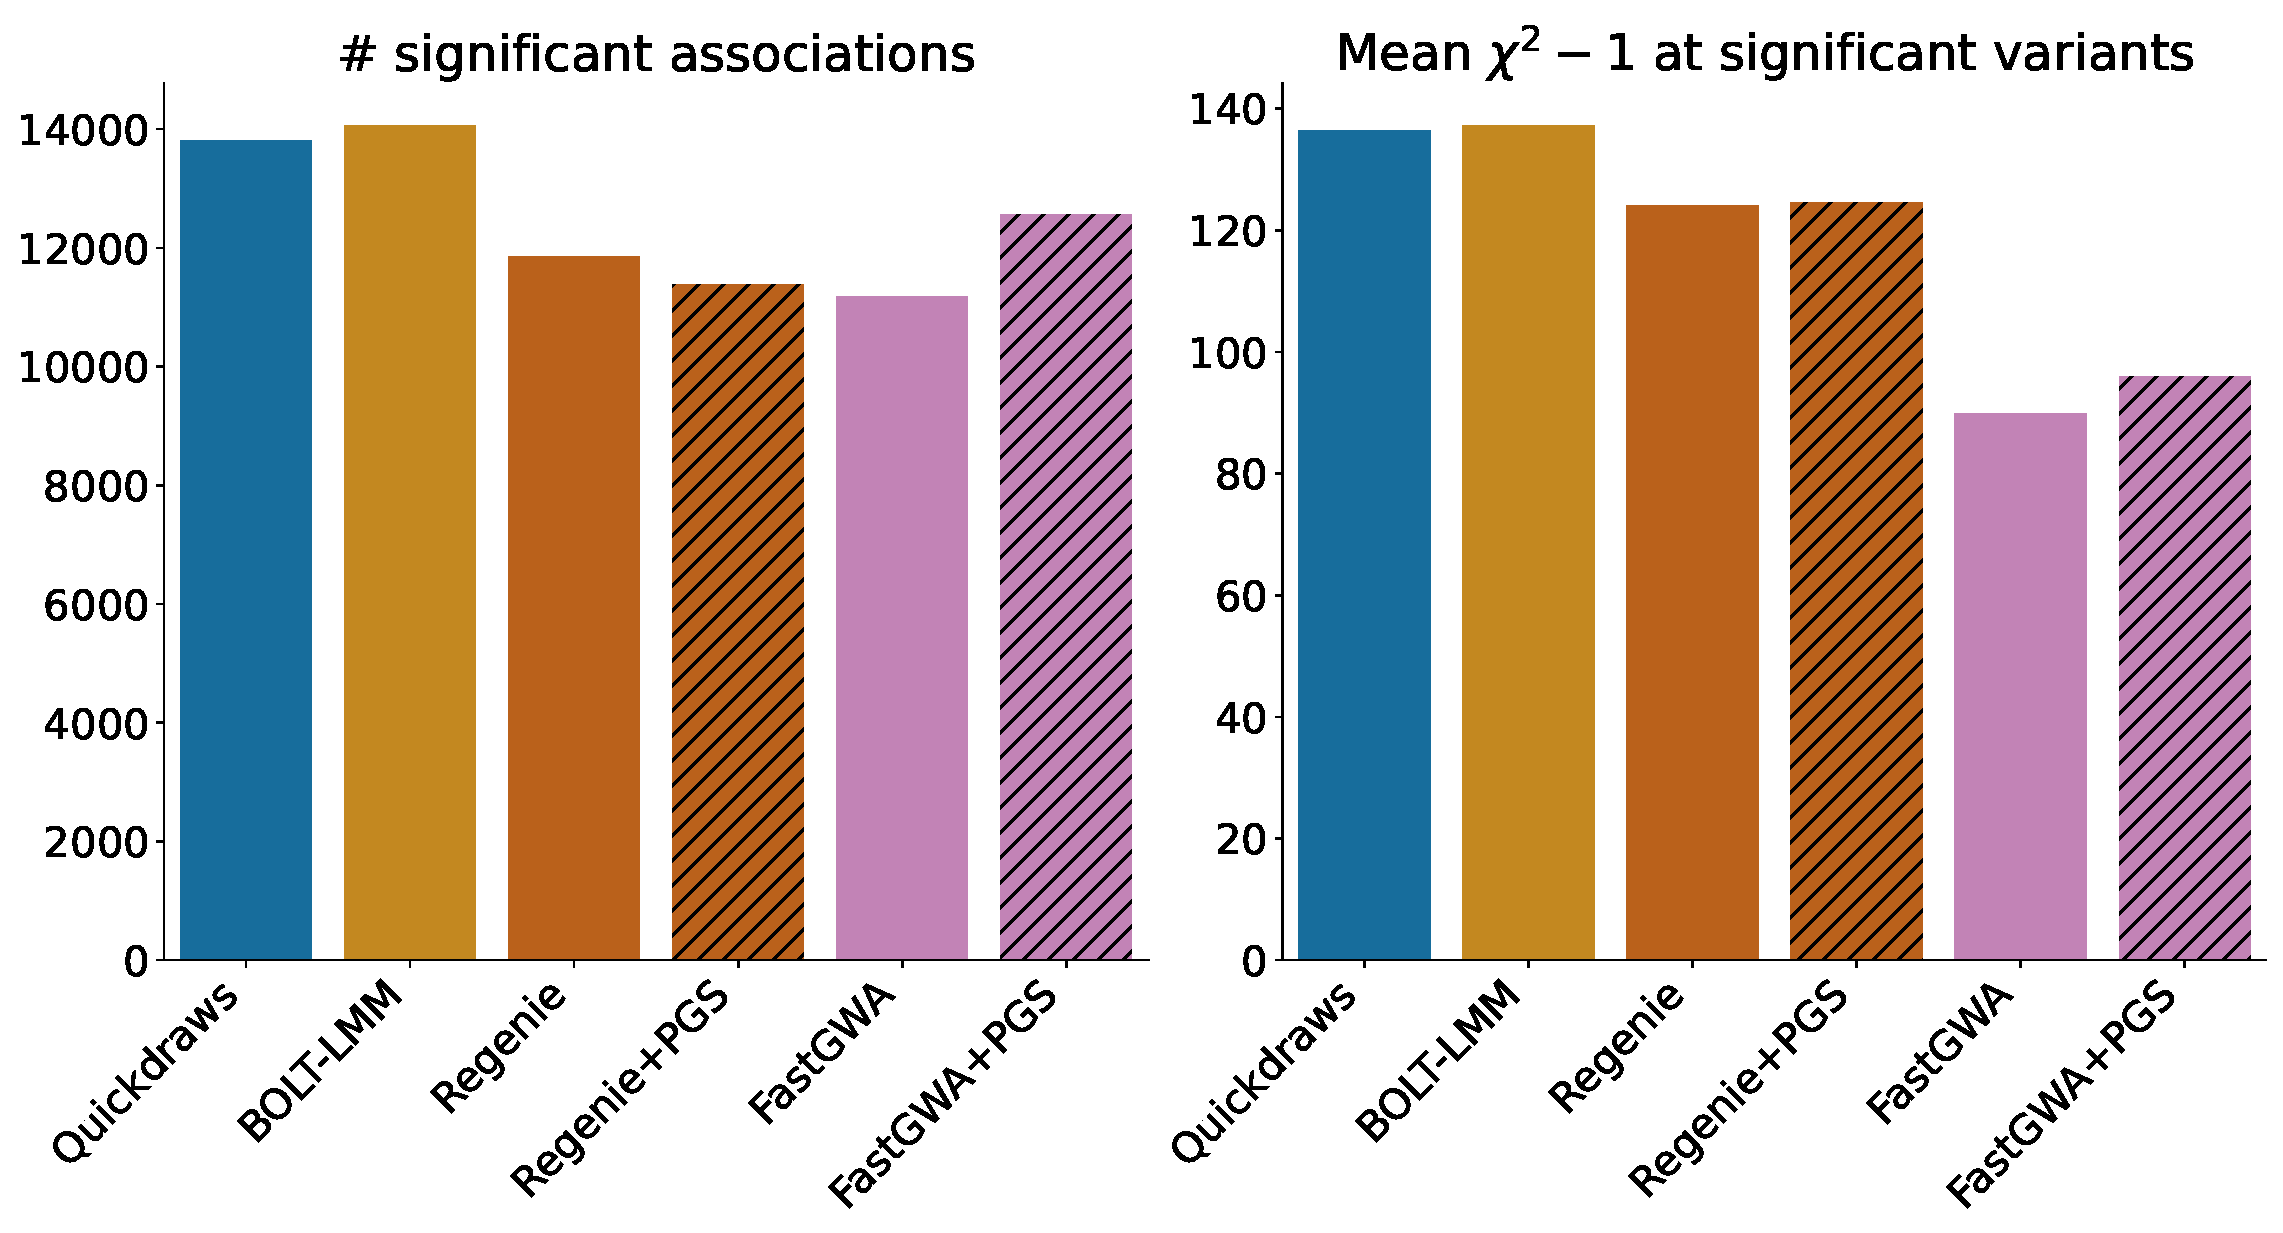
\includegraphics[width=\textwidth]{figures/fig.prs_adjustment.summary.total_loci_noCI.eps}
    % \includegraphics[scale=0.45]{figures/fig.prs_adjustment.summary.mean_loci.eps}
    \caption{\textbf{Effects of PGS-adjustment on association power.}
    %
    (a) Total number of indepedent loci found on chromosomes 1-5, using different GWAS methods with and without PGS adjustment in $79$ UK Biobank quantitative traits.
    %
    (b) Mean $\chi^2$ - 1 at significant variants with and without PGS adjustment for the same traits and regions.
    %
    Significant variants were defined as those with LR-unrel p-value $\leq 5 \times 10^{-8}$.
    %
    FastGWA with PGS adjustment yielded an increase in the number of independent loci (with PGS adjustment, $159.1$; without, $141.6$; paired $t$-test $p=1.9\times 10^{-9}$) and higher mean $\chi^2$-1 at significant variants (with PGS adjustment, $96.0$; without, $89.8$; $p=3.3\times 10^{-11}$).
    %
    Regenie with PGS adjustment yielded fewer independent loci (with PGS adjustment, $144.1$; without, $150.1$; $p=7.4\times 10^{-6}$), and similar mean $\chi^2$ - 1 values (with PGS adjustment, $124.6$; without, $124.1$; $p>0.05$).
    }
    \label{fig:prs_adjustment}
\end{figure}

\clearpage

\subsection{Correction of participation bias}
\label{sec:ch5-ukb-parti-bias}

Quickdraws implements functionality to optionally correct for participation bias when computing association statistics in step 2, using an approach closely related to the one proposed in \cite{schoeler2023participation}.
%
This approach relies on the use of sampling weights, which are computed by considering a range of covariates and are used to up-weight or down-weight individuals estimated to be under-sampled or over-sampled in the study \cite{schoeler2023participation}.
%
Quickdraws takes these weights as input and performs a weighted linear regression, using a Huber-White estimator to compute the variance of the fixed effects in the regression.
%
The test statistics are recalibrated using a weighted linear regression, by matching the effective sample size estimated from a weighted linear regression on an unrelated and homogeneous sample, similar to the unweighted case.
%

%
To apply this approach in the analysis of Table \ref{tab:loci_wgwa}, we analyzed $79$ quantitative traits and $338{,}738$ individuals from the white British subgroup for which all the covariates used in \cite{schoeler2023participation} to estimate sampling weights were available.
%
These covariates included sex, age, education age, alcohol consumption frequency, smoking status, income, household size, employment status, body mass index, overall health, height, urbanization, weight, assessment center, self-reported ethnicity, and years of education.
%
We used the LASSO regression model provided in \cite{schoeler2023participation} to estimate these sampling weights and compared the number of approximately independent loci identified using LDAK with a similar participation bias adjustment but applied on unrelated homogeneous subset of the data.
%

\section{Cost analysis on UK Biobank RAP}
\label{sec:ch5-cost}

We compared the computational efficiency of Quickdraws in large-scale UK Biobank analyses to that of Regenie, FastGWA, SAIGE, and BOLT-LMM, testing the speed and cost of running each method on the UK Biobank's RAP cloud platform.
%
We tested ${\sim}13.3$ million imputed genotypes for association with the $50$ quantitative and $50$ binary traits varying the number of samples between $N=50{,}000$, $N=405{,}088$ and artificially simulated $N=1{,}000k$.
%
We used $458{,}464$ markers for model fitting for Quickdraws, Regenie, and BOLT-LMM and an LD-pruned set of $89{,}177$ markers for SAIGE, and used pre-computed sparse GRM matrices for FastGWA and SAIGE.
%
Unlike current approaches, Quickdraws allows leveraging GPU hardware to speed up the Bayesian regression in the model fitting step.
%
To provide a more detailed overview of computational costs and to optimize the hardware configuration used for each approach, we tested all methods on up to four different RAP machines.

\sloppy
For $N = 50k$, we consider \texttt{mem3\_ssd1\_v2\_x4}, \texttt{mem2\_ssd1\_v2\_x8}, and \texttt{mem1\_ssd1\_v2\_x16}; for $N = 405k$, we consider \texttt{mem2\_ssd1\_v2\_x8}, \texttt{mem2\_ssd1\_v2\_x16}, \texttt{mem1\_ssd1\_v2\_x36}, and \texttt{mem1\_ssd1\_v2\_x72}
\sloppy
%
; for $N = 1{,}000k$, we only consider \texttt{mem1\_ssd1\_v2\_x36}.
Additionally, we use \texttt{mem2\_ssd2\_gpu1\_x8} to run step 1 of Quickdraws on an instance providing a 24GB Nvidia A10G GPU.
%
All the jobs on RAP were run using ``on-demand'' priority.
%
Each method was run using configurations that would optimize performance, where possible, e.g., by allowing multi-threading and supplying files using the most efficient file formats, and all methods were given the same file containing testing variants as input.

BOLT-LMM, FastGWA and SAIGE do not leverage multi-trait parallelization, so we run them for $5$ phenotypes and extrapolate the results for $50$ phenotypes.
%
We also only run BOLT-LMM for one of the three RAP instances, as the large difference in running costs would not to be significantly reduced using other types of hardware.
%
For binary traits and $N = 1{,}000k$, which are more computationally intensive, we run step 2 for Quickdraws, Regenie, and SAIGE using a subset of ${\sim}13.3$ million testing variants, and linearly extrapolate the results.

%
Additionally, Quickdraws allows running the model-fitting step in either high-memory or low-memory mode.
%
The high-memory mode allows for loading the genotype matrix in memory for faster access.
%
The low-memory mode uses a multi-threaded approach to stream the genotype data from disk, decreasing the total memory footprint, while being marginally slower than the high-memory option ($20\%$ slower on the RAP instance we tested).
%
For the analysis in table \ref{tab:speed}, we report the minimal cost across the RAP machines we considered for each method, along with running time and total memory usage computed on a common machine, using the high-memory option for Quickdraws. A more detailed cost analysis can be found in table \ref{tab:speed_quant}, \ref{tab:speed_bin}, \ref{tab:speed_1trait} and \ref{tab:speed_1m}.

\begin{footnotesize}    
\begin{table}[h!]

    \begin{subtable}[h]{\textwidth}
    \centering
    \resizebox{\textwidth}{!}{
    \begin{tabular}{|c|c|c|c|c|c|c|}
    \hline
        Samples & Method & Step 1 & Step 2 & Total time & Total memory* & Cost on RAP** \\ 
        & & (h) & (h) & (h) & (GB) & (£) \\ \hline
        \multirow{1}{*}{50k}
            % & Quickdraws (A100) & 1.3 & 10.3 & 11.6 & 48 (16) & -\\
            & Quickdraws & 9.6 & 9 & 18.6 & 48 (16) & 7.9\\
            & BOLT-LMM & 127 & 671.5 & 798.5 & $<$15 & 158.4\\
            & Regenie & 1.1 & 19.4 & 20.5 & $<$15 & 4.0\\
            & FastGWA & - & 20.2 & 20.2 & $<$15 & 3.6\\
        \hline    
        \multirow{1}{*}{405k}
            % & Quickdraws (A100) & 10.6 & 39.3 & 49.9 & 63 (16) & -\\
            & Quickdraws & 97.7 & 51.5 & 149.3 & 63 (16) & 93.0 \\
            & BOLT-LMM & 1,150 & 7,250 & 8,400 & 46 & 7500.0\\
            & Regenie & 4.7 & 45.3 & 50.0 & $<$15 & 24.2\\
            & FastGWA & - & 128.4 & 128.4 & $<$15 & 37.3\\
        \hline
    \end{tabular}
    }
    \caption{Quantitative traits}
    \end{subtable}
     
     \vspace{5mm}
     
    \begin{subtable}[h]{\textwidth}
    \centering
    \resizebox{\textwidth}{!}{
    \begin{tabular}{|c|c|c|c|c|c|c|}
    \hline
        Samples & Method & Step 1 & Step 2 & Total time & Total memory* & Cost on RAP** \\ 
        & & (h) & (h) & (h) & (GB) & (£) \\ \hline
        \multirow{1}{*}{50k}
            % & Quickdraws (A100) & 1.3 & 10.3 & 11.6 & 48 (16) & -\\
            & Quickdraws & 18.3 & 77.8 & 96.1 & 49 (16) & 25.2 \\
            & SAIGE  & 2.1 & 270.9  & 273 & $<$15 & 47.5 \\
            & Regenie  & 13.1 & 168.9 & 182.0 & $<$15 & 41.0 \\
            & FastGWA  & - & 40.6 & 40.6 & $<$15 & 9.2 \\
        \hline    
        \multirow{1}{*}{405k}
            % & Quickdraws (A100) & 10.6 & 39.3 & 49.9 & 63 (16) & -\\
            & Quickdraws  & 162.7 & 519.7 & 682.3 & 67 (16) & 395.9 \\
            & SAIGE  & 9.0 & 12015.5 & 12024.4 & $<$15 & 2834.9 \\
            & Regenie  & 56 & 813.9 & 869.9 & $<$15 & 506.9 \\
            & FastGWA  & - & 254.1 & 254.1 & $<$15 & 98.1 \\
        \hline
    \end{tabular}
    }
    \caption{Binary traits}
    \end{subtable}
    
    \caption{\textbf{Computational efficiency of Quickdraws for (a) quantitative and (b) binary trait association.} We compare the computational requirements for recent GWAS algorithms with Quickdraws to generate summary statistics for 13.3 million variants and 50 phenotypes with either $N = 50,000$ or $N = 405,088$ and $458,464$ genotyped markers for model fitting ($89,177$ genotyped markers for SAIGE, see Methods); *Total memory includes CPU RAM memory and GPU memory, only Quickdraws requires GPU memory which is reported separately in brackets; **A more detailed cost analysis can be found in table \ref{tab:speed_quant} and \ref{tab:speed_bin} Running times are computed using the same hardware for all methods (mem2\_ssd1\_v2\_x8, with $32$ GB of RAM, $8$-core processor for $N=50k$ and mem1\_ssd1\_v2\_x36, $72$ GB of RAM, $36$-core processor for $N=405k$ datasets).
    }
    \label{tab:speed}
\end{table}
\end{footnotesize}

\section{Discussion}

To fully harness the growing volumes of genomic, phenotypic, and environmental information contained in modern biobanks, existing GWAS algorithms need to optimize a complex trade-off between cost efficiency, statistical power, and robustness.
%
We developed an algorithm for genome-wide association testing, called Quickdraws, that navigates these trade-offs by combining established GWAS paradigms, such as using mixed-effect models \cite{yu2006unified,kang2008efficient,kang2010variance,zhang2010mixed,zhou2012genome,lippert2011fast,segura2012efficient,listgarten2012improved,listgarten2013fast,loh2015efficient,loh2018mixed,jiang2019resource} to handle relatedness and population structure and the use of penalized regression \cite{firth1993bias,mbatchou2021computationally} for binary traits, with recent ideas from Bayesian machine learning, such as stochastic variational inference \cite{graves2011practical,hoffman2013stochastic}, first-order gradient optimizers \cite{robbins1951stochastic,kingma2014adam}, and transfer learning \cite{pan2009survey}.
%
In addition, Quickdraws allows leveraging GPUs, which are available in modern computing platforms and have been widely adopted in machine learning applications to parallelize computationally intensive matrix operations \cite{paszke2017automatic}.
%
Overall, this strategy allows Quickdraws to achieve higher average association power than existing methods in the analysis of binary traits, and to match the association power obtained in quantitative traits by BOLT-LMM, the only other approach that enables modeling of non-infinitesimal architectures.
%
In computational benchmarks using the UK Biobank RAP cloud platform, Quickdraws required a fraction of the computational resources used by BOLT-LMM, with costs comparable to those of scalable methods with lower average association power. 
%
Summary statistics for the traits we analyzed, which comprise $79$ quantitative traits, $50$ self-reported diseases, and $2923$ plasma protein traits, are freely available for download from \href{https://www.stats.ox.ac.uk/publication-data/sge/ppg/quickdraws/}{here}.
%

%%%%%%%%%%%%%%%%%%% Third paragraph %%%%%%%%%%%
The gains in statistical power achieved by Quickdraws are equivalent to analyzing data sets that contain larger sample sizes \cite{yang2011genomic,loh2015efficient,loh2018mixed}, with our simulations showing increases in effective sample size of over $19.2\%$ for traits linked to a few thousands of causal variants.
%
Similarly, our analyses of real traits, in which we focused on quantitative traits and diseases with high heritability and phenotyping rate, yielded more independent association signals than current scalable approaches (e.g., $26.1\%$ and $8.04\%$ increase over Regenie for Height and Mean platelet volume, see tables \ref{tab:loci_qt} and \ref{tab:loci_bt}).
%
Although complex traits are known to be highly polygenic \cite{yengo2022saturated}, their genetic architectures, in particular for molecular traits such as metabolites \cite{kettunen2012genome}, are estimated to be far from a purely infinitesimal model, with large fractions of heritability concentrating in a relatively small set of variants \cite{stahl2012bayesian,zeng2018signatures,weissbrod2020functionally}.
%
As the range of phenotypic measurements available in biobank data sets continues to grow, we therefore expect the increase in computational power that we observed in our analyses to also be observed in broader sets of traits and diseases.
%

\subsection{Sharing and combining posterior effect estimates}

Our analyses demonstrate that, in addition to increasing association power by allowing the computation of a residualized phenotype, the posterior mean estimates of the effect sizes computed during the model fitting step can be used to construct polygenic scores that perform well in held-out individuals compared to those computed from summary association statistics.
%
Therefore, sharing these effect estimates, which we make available for the traits we analyzed (see \href{https://www.stats.ox.ac.uk/publication-data/sge/ppg/quickdraws/}{here}), may facilitate novel downstream analyses.
%
However, compared to the use of summary association statistics, one disadvantage of using posterior effect estimates to construct polygenic scores is the lack of established methodology to combine them across independent cohorts.
%
Developing strategies that allow to meta-analyze these effects across cohorts could open new avenues for the development of federated association and polygenic prediction strategies that preserve high statistical power without the need for sharing individual-level data.
%

% mention federated learning angle, cite two bonnie berger papers 

\subsection{Limitations and future work}

We highlight several current limitations and areas of future work to improve the Quickdraws algorithm.
%
First, Quickdraws leverages modern GPU hardware to speed up the Bayesian regression in the model fitting step and is therefore slower when run on traditional CPU hardware (see Figure \ref{fig:step1_cpu_gpu} for a comparison).
%
GPUs may not be as easily accessible as CPUs, and have higher costs, as evidenced in Table \ref{tab:speed_quant} and \ref{tab:speed_bin}.
%
Our analyses on the RAP cloud platform, however, demonstrates that the overall increase in running costs is not substantial.
%
Furthermore, the extensive use of GPUs in machine learning applications is likely to continue to increase their availability, paving the way for additional GPU-based applications in human genetics.
%
Future work may allow developing a faster CPU-based implementation of Quickdraws.
%
Second, although Quickdraws is well parallelized for the analysis of multiple traits, it currently does not capture the correlations that often exist across these traits.
%
Extending Quickdraws to leverage genetic and environmental correlations is likely to lead to improved performance \cite{korte2012mixed,zhou2014efficient}.
%
%
Third, although we have shown that a strategy based on adjusting for polygenic scores computed within the same sample does not lead to power gains comparable to those achieved by Quickdraws and BOLT-LMM, it is possible that using polygenic scores constructed from larger external cohorts will lead to more substantial power increases \cite{campos2023boosting, jurgens2023adjusting}.
%
Fourth, association analyses have recently been shown to be affected by participation biases \cite{pirastu2021genetic, benonisdottir2023studying}, to which Quickdraws is also susceptible.
%
To mitigate these biases, we implemented the adjustment strategy proposed in \cite{schoeler2023participation} in step 2 of the Quickdraws algorithm (as described in section \ref{sec:ch5-ukb-parti-bias}).
%
However, further work will be needed to incorporate this adjustment in step 1 of the algorithm.
%
Despite these current limitations and avenues for future development, we believe that Quickdraws will provide a useful tool for large-scale GWAS, demonstrating the promise of leveraging modern machine learning methodology to improve statistical power and efficiency in these analyses.

\begin{figure}
    \centering
    \includegraphics[width=0.75\textwidth]{figures/step1_running_time_cost.pdf}
    \caption{\textbf{Computational performance of Quickdraws on different computing architectures.} We assessed the running time and cost associated with Quickdraws' model fitting step (Step 1) across varying numbers of samples ($N$) and phenotypes ($P$). Performance was compared for three architectures: an Nvidia A10G GPU node on the UK Biobank Research Analysis Platform (RAP) (\texttt{mem2\_ssd2\_gpu1\_x8}), a 14-core MacBook Pro equipped with the Apple M3 chip, and an 8-core CPU node on the UK Biobank RAP (\texttt{mem2\_ssd1\_v2\_x8}). Running costs were calculated only for the GPU and CPU nodes on the RAP.}
    \label{fig:cpu_vs_gpu_vs_mac}
\label{fig:step1_cpu_gpu}
\end{figure}


%% APPENDICES %% 
% Starts lettered appendices, adds a heading in table of contents, and adds a
%    page that just says "Appendices" to signal the end of your main text.
\startappendices
% Add or remove any appendices you'd like here:
\chapter{\label{app:1-KL_divergence}Additional proofs}

\minitoc

\section{KL-divergence for non-overlapping mixture distributions}
\label{sec:kl_div}

\pgfmathdeclarefunction{gauss}{2}{%
  \pgfmathparse{1/(#2*sqrt(2*pi))*exp(-((x-#1)^2)/(2*#2^2))}%
}

\begin{figure}[h!]
\centering
\begin{minipage}{0.45\textwidth}
\centering
\begin{tikzpicture}
\begin{axis}[every axis plot post/.append style={
  mark=none,samples=500,smooth,domain=-11:11},xlabel = {Posterior distribution}, legend entries = {$f_1$, $f_2$}, 
  axis x line*=bottom, 
  axis y line*=left, 
  enlargelimits=upper] 
  \addplot {gauss(-5,0.4)};
  \addplot {gauss(7.5,0.6)};
  \coordinate (a) at (axis cs:5, 0.1);
  \draw[red, dashed, thick](a |- current plot begin) -- (a);
  \coordinate (a) at (axis cs:10, 0.1);
  \draw[red, dashed, thick](a |- current plot begin) -- (a);
  \coordinate (a) at (axis cs:-10, 0.1);
  \draw[blue, dashed, thick](a |- current plot begin) -- (a);
  \coordinate (a) at (axis cs:0, 0.1);
  \draw[blue, dashed, thick](a |- current plot begin) -- (a);
\end{axis}
\end{tikzpicture}
\end{minipage}
\hfill
\begin{minipage}{0.45\textwidth}
\centering
\begin{tikzpicture}
\begin{axis}[every axis plot post/.append style={
  mark=none,samples=500,smooth,domain=-11:11},xlabel = {Prior distribution}, legend entries = {$g_1$, $g_2$},
  axis x line*=bottom, 
  axis y line*=left, 
  enlargelimits=upper] 
  \addplot {gauss(-4,0.43)};
  \addplot {gauss(7,0.43)};
  \coordinate (a) at (axis cs:5, 0.1);
  \draw[red, dashed, thick](a |- current plot begin) -- (a);
  \coordinate (a) at (axis cs:10, 0.1);
  \draw[red, dashed, thick](a |- current plot begin) -- (a);
  \coordinate (a) at (axis cs:-10, 0.1);
  \draw[blue, dashed, thick](a |- current plot begin) -- (a);
  \coordinate (a) at (axis cs:0, 0.1);
  \draw[blue, dashed, thick](a |- current plot begin) -- (a);
\end{axis}
\end{tikzpicture}
\end{minipage}
\end{figure}
\textbf{Theorem 1:}
%
Let $q = \sum^{N}_i \pi_i f_i$ be a mixture of non-overlapping distributions, i.e., $S_i \cap S_j = \emptyset, \forall i \neq j$, where $S_i$ is the support of distribution $f_i$.
%
If $p$ is a probability distribution and can be represented as a mixture of non-overlapping distributions with the same support as $f_i$, i.e., $p = \sum^{N}_i \pi'_i g_i$ and support of $g_i$ = support of $f_i$, the KL divergence between $q$ and $p$ can be simplified as follows:

\begin{equation}
KL(q || p) = \sum^N_i \left( \pi_i KL (f_i || g_i) + \pi_i \log (\pi_i) - \pi_i \log(\pi'_i) \right)
\end{equation}

%

%
\textbf{Proof:} 
Assuming $q$ is $0$ outside $\cup^N_i S_i$, we can write the integral as

\begin{align}
    KL (q || p) &= \int q \log (q) - q \log (p) = \sum^N_i \int_{S_i} q \log (q) - q \log (p) \nonumber \\
    &= \sum^N_i \int_{S_i} \left(\sum^{N}_i \pi_i f_i \right)\log \left(\sum^{N}_i \pi_i f_i\right) - \left( \sum^{N}_i \pi_i f_i\right) \log \left(\sum^{N}_i \pi'_i g_i\right).
\end{align}

Because $S_i \cap S_j = \emptyset, \forall i \neq j$, we can simplify as

\begin{align}
   KL (q || p) &=  \sum^N_i \int_{S_i} \pi_i f_i \log(\pi_i f_i) - \pi_i f_i \log(\pi'_i g_i) \nonumber \\
   &= \sum^N_i \pi_i \left( \int_{S_i} f_i \log(f_i) -  f_i \log(g_i) \right) + \sum^N_i \left( \pi_i log (\pi_i) \int_{S_i} f_i - \pi_i log (\pi'_i) \int_{S_i} f_i \right) \nonumber \\
   &= \sum^N_i \pi_i \left( \int_{S_i} f_i \log(f_i) -  f_i \log(g_i) \right) + \sum^N_i \left(\pi_i log (\pi_i) - - \pi_i log (\pi'_i) \right) \nonumber \\
   &= \sum^N_i \left( \pi_i KL (f_i || g_i) + \pi_i \log (\pi_i) - \pi_i \log(\pi'_i) \right)
\end{align}


\chapter{\label{app:1-KL_divergence}Additional figures and tables}

\minitoc

\section{Additional figures}
\label{sec:additional_figures}

\begin{figure}
    \centering
    \includegraphics[width=\textwidth]{figures/gb_merge_sanity_check.png}
    \caption{\textbf{Comparison of Allele Frequencies between HGDP+1000GP and Ancient Samples.} We analyze biallelic SNPs on chromosome 20 within the masked regions. The comparison includes union (``all sites'') and intersection (``overlapping sites'') of SNPs in the two datasets seperately.}
    \label{fig:gb-sanity-check}
\end{figure}

\begin{figure}[h!]
    \centering
    \includegraphics[width=\textwidth]{figures/sim_calibration/popstructure_fpr.pdf}
    \caption{
    \textbf{Summary of calibration in simulations with varying levels of population structure.}
    %
    False positive rate (FPR) at a significance threshold of $\alpha \in \{0.05, 0.0005\}$, calculated as the fraction of variants on even chromosomes with p-value lower than $\alpha$.
    %
    The line inside each box indicates the median value, the central box indicates the interquartile range, whiskers indicate data up to $1.5$ times the IQR, and outliers are shown as separate points.
    %
    A description of the group labels (GB-unrel, EUR, PAS) is provided in section \ref{sec:ch5-sim-design}.
    }
    \label{fig:sim_calib_pop}
\end{figure}

\newpage

\begin{figure}[h!]
    \centering
    \includegraphics[width=\textwidth]{figures/sim_calibration/relatedness_fpr.pdf}
    \caption{\textbf{Summary of calibration in simulations with varying levels of relatedness.}
    %
    False positive rate (FPR) at a significance threshold of $\alpha \in \{0.05, 0.0005\}$, calculated as the number of variants on even chromosomes with p-value lower than $\alpha$.
    %
    The line inside each box indicates the median value, the central box indicates the interquartile range, whiskers indicate data up to $1.5$ times the IQR, and outliers are shown as separate points.
    %
    GB-unrel refers to simulations including only unrelated British individuals, GB-rel-ukb refers to randomly sampling from the related white British subset, GB-rel refers to the default relatedness setting with $3.4 \times$ more relative pairs compared to the UK Biobank, and GB-rel+ refers to the extreme relatedness case of $7.3 \times$ and $4.8 \times$ more first and second degree relative pairs compared to the UK Biobank.
    %
    The prevalence of binary traits was fixed at 10\%.
    }
    \label{fig:sim_calib_rel}
\end{figure}

\begin{figure}[h!]
    \centering
    \includegraphics[width=\textwidth]{figures/sim_calibration/mog_fpr.pdf}
    \caption{
    \textbf{Summary of calibration in simulations with varying causal effect distributions: }
    %
    The first two rows correspond to causal effects simulated from a mixture of two Gaussian. 
    %
    Polygenicity refers to the proportion corresponding to the Gaussian with higher variance, and f refers to the fraction of total variance explained by the Gaussian with lower variance.
    %
    False positive rate (FPR) at a significance threshold of $\alpha \in \{0.05, 0.0005\}$, calculated as the fraction of variants on even chromosomes with p-value lower than $\alpha$.
    %
    The line inside each box indicates the median value, the central box indicates the interquartile (IQR) range, whiskers indicate data up to $1.5$ times the IQR, and outliers are shown as separate points.
    %
    \label{fig:sim_calib_mog}
    }
\end{figure}

\begin{figure}[h!]
    \centering
    \includegraphics[width=\textwidth]{figures/sim_power/qt_power.pdf}
    
    \caption{\textbf{Summary of statistical power in simulations for quantitative traits.}
    %
    We measure the normalized causal $\chi^2$ at top $1{,}000$ and top $10{,}000$ causal variants.
    %
    To correct for confounding, the causal $\chi^2$ is normalized by the average $\chi^2$ at null variants on even chromosomes.
    %
    The line inside each box indicates the median value, the central box indicates the interquartile range, whiskers indicate data up to $1.5$ times the IQR, and outliers are shown as separate points.
    %
    A description of the group labels (GB-unrel, GB-rel, GB-rel+, EUR) is provided in section \ref{sec:ch5-sim-design}.
    \label{fig:sim_power_qt}
    }
\end{figure}

\begin{figure}[h!]
    \centering
    \includegraphics[width=\textwidth]{figures/sim_power/bt_power.pdf}
    
    \caption{\textbf{
    %
    Summary of statistical power in simulations for binary traits.}
    %
    We measure the normalized causal $\chi^2$ at top $1{,}000$ and top $10{,}000$ causal variants.
    %
    To correct for confounding, the causal $\chi^2$ is normalized by the average $\chi^2$ at null variants on even chromosomes.
    %
    The line inside each box indicates the median value, the central box indicates the interquartile range, whiskers indicate data up to $1.5$ times the IQR, and outliers are shown as separate points.
    %
    A description of the group labels (GB-unrel, GB-rel, EUR) is provided in the section \ref{sec:ch5-sim-design}.
    \label{fig:sim_power_bt}
    }
\end{figure}

\begin{figure}[h!]
    \centering
    \includegraphics[width=\textwidth]{figures/sim_power/mog_power.pdf}
    \caption{
    \textbf{
    %
    Summary of statistical power in simulations with varying causal effect distributions.}
    %
    The first two rows correspond to causal effects simulated from a mixture of two Gaussian. 
    %
    Polygenicity refers the proportion corresponding to the Gaussian with higher variance, and f refers to the fraction of total variance explained by the Gaussian with lower variance.
    %
    We measure the normalized causal $\chi^2$ at top $1{,}000$ and top $10{,}000$ causal variants.
    %
    To correct for confounding, the causal $\chi^2$ is normalized by the average $\chi^2$ at null variants on even chromosomes.
    %
    The line inside each box indicates the median value, the central box indicates the interquartile range (IQR), whiskers indicate data up to $1.5$ times the IQR, and outliers are shown as separate points.
    }
    %
    \label{fig:sim_power_mog}
\end{figure}

\begin{figure}[h!]
    \centering
    \includegraphics[scale=0.425]{figures/manhattan_bin/legend.png}
    \begin{subfigure}{.5\textwidth}
    \includegraphics[width=\textwidth]{figures/manhattan_bin/fastgwa_400k1.png}
    \end{subfigure}%
    \begin{subfigure}{.5\textwidth}
    \includegraphics[width=\textwidth]{figures/manhattan_bin/fastgwa_400k16.png}
    \end{subfigure}
    \begin{subfigure}{.5\textwidth}
    \includegraphics[width=\textwidth]{figures/manhattan_bin/regenie_400kAsthma.png}
    \end{subfigure}%
    \begin{subfigure}{.5\textwidth}
    \includegraphics[width=\textwidth]{figures/manhattan_bin/regenie_400kBasal_cell_carcinoma.png}
    \end{subfigure}
    \begin{subfigure}{.5\textwidth}
    \includegraphics[width=\textwidth]{figures/manhattan_bin/imputed_bgen_bolt_0.sumstats.gz.png}
    \end{subfigure}%
    \begin{subfigure}{.5\textwidth}
    \includegraphics[width=\textwidth]{figures/manhattan_bin/imputed_bgen_bolt_1.sumstats.gz.png}
    \end{subfigure}
    \begin{subfigure}{.5\textwidth}
    \includegraphics[width=\textwidth]{figures/manhattan_bin/qd_Asthma.sumstats.gz.png}
    \caption{}
    \end{subfigure}%
    \begin{subfigure}{.5\textwidth}
    \includegraphics[width=\textwidth]{figures/manhattan_bin/qd_Basal_cell_carcinoma.sumstats.gz.png}
    \caption{}
    \end{subfigure}
    \caption{\textbf{Manhattan plots for two binary traits.}
    %
    (a) Asthma (prevalence $= 0.119$) and (b) Basal cell carcinoma (prevalence $= 0.012$).
    %
    ${\sim}13.3$ million variants were tested.
    %
    Red lines indicate a genome-wide significance threshold of $ P = 5 \times 10^{-8}$ and the green line indicates $P = 1 \times 10^{-20}$.
    }
    \label{fig:qd_man_bin1}
\end{figure}

\begin{figure}[h!]
    \centering
    \includegraphics[scale=0.425]{figures/manhattan_bin/legend.png}
    \begin{subfigure}{.5\textwidth}
    \includegraphics[width=\textwidth]{figures/manhattan_bin/fastgwa_400k17.png}
    \end{subfigure}%
    \begin{subfigure}{.5\textwidth}
    \includegraphics[width=\textwidth]{figures/manhattan_bin/fastgwa_400k22.png}
    \end{subfigure}
    \begin{subfigure}{.5\textwidth}
    \includegraphics[width=\textwidth]{figures/manhattan_bin/regenie_400kCoeliac_disease.png}
    \end{subfigure}%
    \begin{subfigure}{.5\textwidth}
    \includegraphics[width=\textwidth]{figures/manhattan_bin/regenie_400kVitiligo.png}
    \end{subfigure}
    \begin{subfigure}{.5\textwidth}
    \includegraphics[width=\textwidth]{figures/manhattan_bin/imputed_bgen_bolt_2.sumstats.gz.png}
    \end{subfigure}%
    \begin{subfigure}{.5\textwidth}
    \includegraphics[width=\textwidth]{figures/manhattan_bin/imputed_bgen_bolt_3.sumstats.gz.png}
    \end{subfigure}
    \begin{subfigure}{.5\textwidth}
    \includegraphics[width=\textwidth]{figures/manhattan_bin/qd_Coeliac_disease.sumstats.gz.png}
    \caption{}
    \end{subfigure}%
    \begin{subfigure}{.5\textwidth}
    \includegraphics[width=\textwidth]{figures/manhattan_bin/qd_Vitiligo.sumstats.gz.png}
    \caption{}
    \end{subfigure}
    \caption{\textbf{Manhattan plots for two binary traits.}
    %
    (a) Celiac disease (prevalence $= 0.0047$) and (b) Vitiligo (prevalence $= 0.0005$).
    %
    ${\sim}13.3$ million variants were tested.
    %
    Red lines indicate a genome-wide significance threshold of $ P = 5 \times 10^{-8}$ and the green line indicates $P = 1 \times 10^{-20}$.    }
    \label{fig:qd_man_bin2}
\end{figure}


\begin{figure}[h!]
    \centering
    \includegraphics[scale=0.425]{figures/manhattan_quant/legend.png}
    \begin{subfigure}{.5\textwidth}
    \includegraphics[width=\textwidth]{figures/manhattan_quant/imputed_fastgwa0.png}
    \end{subfigure}%
    \begin{subfigure}{.5\textwidth}
    \includegraphics[width=\textwidth]{figures/manhattan_quant/imputed_fastgwa3.png}
    \end{subfigure}
    \begin{subfigure}{.5\textwidth}
    \includegraphics[width=\textwidth]{figures/manhattan_quant/regenie_400k_Eosinophill_count.regenie.png}
    \end{subfigure}%
    \begin{subfigure}{.5\textwidth}
    \includegraphics[width=\textwidth]{figures/manhattan_quant/regenie_400k_Haemoglobin_concentration.regenie.png}
    \end{subfigure}
    \begin{subfigure}{.5\textwidth}
    \includegraphics[width=\textwidth]{figures/manhattan_quant/qd_Eosinophill_count.sumstats.gz.png}
    \caption{}
    \end{subfigure}%
    \begin{subfigure}{.5\textwidth}
    \includegraphics[width=\textwidth]{figures/manhattan_quant/qd_Haemoglobin_concentration.sumstats.gz.png}
    \caption{}
    \end{subfigure}
    \caption{\textbf{Manhattan plots for two quantitative traits.}
    %
    (a) Eosinophil count (RHE-me $h^2 = 0.213$) and (b) Haemoglobin concentration (RHE-mc $h^2 = 0.158$).
    %
    ${\sim}13.3$ million variants were tested.
    %
    Red lines indicate a genome-wide significance threshold of $ P = 5 \times 10^{-8}$ and the green line indicates $P = 1 \times 10^{-20}$.
    }
    \label{fig:qd_man_quant1}
\end{figure}

\begin{figure}[h!]
    \centering
    \includegraphics[scale=0.425]{figures/manhattan_quant/legend.png}
    \begin{subfigure}{.5\textwidth}
    \includegraphics[width=\textwidth]{figures/manhattan_quant/imputed_fastgwa8.png}
    \end{subfigure}%
    \begin{subfigure}{.5\textwidth}
    \includegraphics[width=\textwidth]{figures/manhattan_quant/imputed_fastgwa12.png}
    \end{subfigure}
    \begin{subfigure}{.5\textwidth}
    \includegraphics[width=\textwidth]{figures/manhattan_quant/regenie_400k_Lymphocyte_percentage.regenie.png}
    \end{subfigure}%
    \begin{subfigure}{.5\textwidth}
    \includegraphics[width=\textwidth]{figures/manhattan_quant/regenie_400k_Mean_platelet_thrombocyte_volume.regenie.png}
    \end{subfigure}
    \begin{subfigure}{.5\textwidth}
    \includegraphics[width=\textwidth]{figures/manhattan_quant/qd_Lymphocyte_percentage.sumstats.gz.png}
    \caption{}
    \end{subfigure}%
    \begin{subfigure}{.5\textwidth}
    \includegraphics[width=\textwidth]{figures/manhattan_quant/qd_Mean_platelet_thrombocyte_volume.sumstats.gz.png}
    \caption{}
    \end{subfigure}
    \caption{\textbf{Manhattan plots for two quantitative traits.}
    %
    (a) Lymphocyte percentage (RHE-mc $h^2 = 0.196$) and (b) Mean platelet volume (RHE-mc $h^2 = 0.448$).
    %
    ${\sim}13.3$ million variants were tested.
    %
    Red lines indicate a genome-wide significance threshold of $ P = 5 \times 10^{-8}$ and the green line indicates $P = 1 \times 10^{-20}$.
    }
    \label{fig:qd_man_quant2}
\end{figure}


\clearpage

\section{Additional tables}
\label{sec:additional_tables}

\begin{longtable}{|l|c|c|c|}
\caption{\textbf{Coverage Data Across Different Regions}} \\
\hline
\textbf{ID} & \textbf{Date} & \textbf{Country} & \textbf{Coverage} \\
\hline
\endfirsthead

\caption{\textit{(Continued)}} \\
\hline
\textbf{ID} & \textbf{Date} & \textbf{Country} & \textbf{Coverage} \\
\hline
\endhead

\hline
\multicolumn{4}{r}{\textit{Continued on next page}} \\
\endfoot

\hline
\endlastfoot

AltaiNeandertal & 110,450 & Russia & 52.0 \\ \hline
Vindija & 41,950 & Croatia & 30.0 \\ \hline
Chagyrskaya & 80,000 & Russia & 27.0 \\ \hline
Denisova & 63,900 & Russia & 31.0 \\ \hline
WC1 & 9,219 & Iran & 10.4 \\ \hline
PB675 & 5,416 & Ireland & 15.9 \\ \hline
JP14 & 5,497 & Ireland & 16.6 \\ \hline
SRA62 & 5,979 & Ireland & 13.2 \\ \hline
rath1 & 3,906 & Ireland & 11.6 \\ \hline
bally & 5,132 & Ireland & 11.3 \\ \hline
Yamnaya & 4,890 & Kazakhstan & 25.2 \\ \hline
BOT2016 & 5,450 & Kazakhstan & 13.6 \\ \hline
Ust\_Ishim & 45,020 & Russia & 42.0 \\ \hline
SF12 & 8,895 & Sweden & 65.2 \\ \hline
KH150622 & 3,350 & Germany & 18.2 \\ \hline
KH150623 & 3,350 & Germany & 17.1 \\ \hline
KH150620 & 3,350 & Germany & 16.3 \\ \hline
KK1 & 9,678 & Georgia & 11.3 \\ \hline
I0018 & 7,140 & Germany & 19.0 \\ \hline
I0001 & 8,025 & Luxembourg & 20.1 \\ \hline
I10871 & 7,890 & Cameroon & 18.5 \\ \hline
I5950 & 4,472 & Ethiopia & 11.3 \\ \hline
Klein7 & 7,122 & Austria & 11.3 \\ \hline
Asp6 & 7,524.5 & Austria & 12.1 \\ \hline
Ess7 & 6,975 & Germany & 12.3 \\ \hline
Herx & 7,078.5 & Germany & 11.5 \\ \hline
Dil16 & 7,116.5 & Germany & 10.6 \\ \hline
Nea2 & 8,098 & Greece & 12.5 \\ \hline
Nea3 & 8,183.5 & Greece & 11.6 \\ \hline
VC3-2 & 7,495.5 & Serbia & 11.2 \\ \hline
STAR1 & 7,532.5 & Serbia & 10.6 \\ \hline
LEPE52 & 7,812 & Serbia & 12.4 \\ \hline
LEPE48 & 7,939.5 & Serbia & 10.9 \\ \hline
VLASA7 & 8,552 & Serbia & 15.2 \\ \hline
VLASA32 & 9,604.5 & Serbia & 12.7 \\ \hline
Bar25 & 8,294.5 & Turkey & 12.7 \\ \hline
AKT16 & 8,547.5 & Turkey & 12.3 \\ \hline
USR1 & 11,435 & USA & 17.0 \\ \hline
Sumidouro5 & 10,405 & Brazil & 13.6 \\ \hline
Lovelock3 & 627 & USA & 18.1 \\ \hline
Lovelock2 & 1,880 & USA & 14.4 \\ \hline
AHUR\_2064 & 10,970 & USA & 17.9 \\ \hline
Anzick & 12,649 & USA & 14.0 \\ \hline
new001 & 418 & South Africa & 11.1 \\ \hline
ela001 & 493 & South Africa & 10.5 \\ \hline
baa001 & 1,909 & South Africa & 12.9 \\ \hline
2H11 & 5,163 & France & 23.6 \\ \hline
2H10 & 5,166 & France & 13.8 \\ \hline
Kolyma1 & 9,786 & Russia & 15.0 \\ \hline
Yana1 & 31,950 & Russia & 24.3 \\ \hline
Sunghir3 & 34,093 & Russia & 12.0 \\ \hline
atp016 & 4,971 & Spain & 15.3 \\ \hline
atp002 & 4,746 & Spain & 11.3
\label{tab:gb_ancient_samples}
\end{longtable}


\begin{longtable}{|c|c|c|c|}
\caption{\textbf{Quantitative traits analyzed.} Quantitative traits analyzed, including RHE-MC $h^2$ estimates and sample sizes (N).} \label{tab:ukb_qt_traits} \\
\hline
\textbf{UKBB ID} & \textbf{Phenotype} & \textbf{$h^2$} & \textbf{N}   \\
\hline
\endfirsthead
\caption{\textit{(Continued)}}\\
\hline
\textbf{UKBB ID} & \textbf{Phenotype} & \textbf{$h^2$} & \textbf{N}  \\
\hline
\endhead
\hline
\multicolumn{4}{r}{\textit{Continued on next page}} \\
\endfoot
\hline
\endlastfoot
30850 &  Testosterone & 0.03 & 355373 \\
1438 & Bread intake & 0.053 & 396396\\
874 & Duration of walks & 0.054 & 346657\\
30750 &  Glucose & 0.088 & 359138 \\
2217 & Age started wearing glasses & 0.092 & 349337\\
30710 &  Mean corp. haemoglobin conc. & 0.101 & 398336 \\
30810 &  Phosphate & 0.149 & 358861 \\
30790 &  LDL direct & 0.152 & 390888  \\
3064 & Peak expiratory flow (PEF) & 0.152 & 370024\\
30690 &  Cholesterol & 0.157 & 391567 \\
30760 &  Haemoglobin conc & 0.158 & 398342 \\
30020 &  Haematocrit \% & 0.161 & 398343 \\
46 & Hand grip strength (left) & 0.162 & 403800\\
47 & Hand grip strength (right) & 0.164 & 403850\\
30600 &  Albumin & 0.168 & 359528 \\
30670 &  Urea & 0.172 & 391307 \\
30680 &  Calcium & 0.177 & 359391 \\
30650 &  Asp-aminotransferase & 0.178 & 390183 \\
30860 &  Total protein & 0.188 & 359122 \\
4079 & Diastolic blood pressure & 0.188 & 379181\\
30640 &  Apolipoprotein B & 0.189 & 389718 \\
30200 &  Neutrophill \% & 0.19 & 397665 \\
4080 & Systolic blood pressure & 0.192 & 379174 \\
102 & Pulse rate & 0.194 & 379181 \\
30120 &  Lymphocyte \% & 0.196 & 397665 \\
30210 &  Creatinine & 0.198 & 391377  \\
30830 &  SHBG & 0.2 & 356165 \\
30880 &  Urate & 0.206 & 391102 \\
30630 &  Apolipoprotein A & 0.213 & 357411 \\
30730 &  Eosinophill count & 0.213 & 397661 \\
30180 &  Lipoprotein A & 0.22 & 312270 \\
30140 &  Neutrophill count & 0.22 & 397661  \\
30190 &  Monocyte \% & 0.221 & 397665 \\
30870 &  Triglycerides & 0.234 & 391260 \\
30740 &  Gamma glutamyltransferase & 0.24 & 391372 \\
30700 &  C-reactive protein & 0.241 & 390752 \\
20257 & Forced vital capacity (FVC) Z-score & 0.242 & 328403 \\
30030 &  Glycated haemoglobin & 0.245 & 391597  \\
30290 &  HDL cholesterol & 0.248 & 359370 \\
30150 &  Eosinophill \% & 0.251 & 397665 \\
30130 &  Monocyte count & 0.253 & 397661 \\
30780 &  Immature reticulocyte fraction & 0.26 & 391990 \\
30250 &  Reticulocyte count & 0.26 & 392210 \\
20256 & Forced expiratory volume (FEV1) Z-score & 0.263 & 328403\\
30070 &  Red blood cell distribution width & 0.264 & 398342  \\
30260 &  Mean reticulocyte vol & 0.266 & 392211 \\
30240 &  Reticulocyte \% & 0.267 & 392210 \\
20258 & FEV1/FVC ratio Z-score & 0.269 & 328403\\
30050 &  Lymphocyte count & 0.269 & 397661 \\
48 & Waist circumference & 0.277 & 404969\\
30010 &  Red blood cell count & 0.279 & 398343 \\
30610 &  Alkaline phosphatase & 0.279 & 391586 \\
30770 &  High light scatter reticulocyte count & 0.289 & 391989 \\
30280 &  IGF-1 & 0.29 & 389525 \\
30270 &  Mean sphered cell vol & 0.293 & 391990 \\
23115 & Leg fat \% (left) & 0.294 & 399130\\
23111 & Leg fat \% (right) & 0.294 & 399151\\
30110 &  Platelet distribution width & 0.296 & 398153 \\
23127 & Trunk fat \% & 0.302 & 398940\\
23119 & Arm fat \% (right) & 0.302 & 399098\\
23123 & Arm fat \% (left) & 0.305 & 399037\\
30300 &  High light scatter reticulocyte \% & 0.306 & 391990 \\
23099 & Body fat \% & 0.310 & 398955\\
49 & Hip circumference & 0.318 & 404972\\
30090 &  Platelet crit & 0.326 & 398154 \\
30840 &  Total bilirubin & 0.327 & 389995 \\
23110 & Impedance of arm (left) & 0.331 & 399149\\
23109 & Impedance of arm (right) & 0.331 & 399133 \\
23128 & Trunk fat mass & 0.331 & 398918 \\
21001 & Body mass index (BMI) & 0.348 & 405010\\
23106 & Impedance of whole body & 0.367 & 399144 \\
30080 &  Platelet count & 0.373 & 398339   \\
21002 & Weight & 0.381 & 405018 \\
30040 &  Mean corp. vol & 0.414 & 398342  \\
23105 & Basal metabolic rate & 0.419 & 399169\\
23102 & Whole body water mass & 0.428 & 399179 \\
30060 &  Mean corp. haemoglobin & 0.432 & 398339 \\
30100 &  Mean platelet vol & 0.448 & 398334 \\
50 & Standing height & 0.745 & 405035 \\
\end{longtable}

\begin{longtable}{|c|c|c|c|}
\caption{\textbf{Self-reported disease traits analyzed.} Self-reported disease traits analyzed, including their disease code and prevalence.} \label{tab:ukb_bt_traits}
\\
\hline
\textbf{UKBB ID} & \textbf{Disease ID} & \textbf{Phenotype} & \textbf{Prevalence}   \\
\hline
\endfirsthead
\caption{\textit{(Continued)}}\\
\hline
\textbf{UKBB ID} & \textbf{Disease ID} & \textbf{Phenotype} & \textbf{Prevalence}   \\
\hline
\endhead
\hline
\multicolumn{4}{r}{\textit{Continued on next page}} \\
\endfoot
\hline
\endlastfoot
20002 & 1065 & Hypertension & 0.2740\\
20002 & 1473 & High cholestrol & 0.1400\\
20002 & 1111 & Asthma & 0.1190\\
20002 & 1465 & Osteoarthritis & 0.0946\\
20002 & 1387 & Hayfever & 0.0667\\
20002 & 1286 & Depression & 0.0649\\
20002 & 1138 & Gastric reflux & 0.0529\\
20002 & 1226 & Hypothyroidism & 0.0518\\
20002 & 1220 & Diabetes & 0.0421\\
20002 & 1265 & Migraine & 0.0343\\
20002 & 1074 & Angina & 0.0335\\
20002 & 1452 & Eczema & 0.0320\\
20002 & 1474 & Hiatus hernia & 0.0266\\
20002 & 1075 & Heart attack & 0.0247\\
20001 & 1002 & Breast cancer & 0.0241\\
20002 & 1094 & Deep venous thrombosis & 0.0210\\
20002 & 1162 & Cholelithiasis & 0.0188\\
20002 & 1294 & Back problem & 0.0183\\
20002 & 1396 & Enlarged prostate & 0.0183\\
20002 & 1309 & Osteoporosis & 0.0182\\
20002 & 1287 & Anxiety & 0.0182\\
20002 & 1351 & Uterine fibroids & 0.0170\\
20002 & 1538 & Arthritis nos & 0.0148\\
20002 & 1113 & Emphysema & 0.0142\\
20002 & 1458 & Diverticulitis & 0.0137\\
20002 & 1453 & Psoriasis & 0.0131\\
20002 & 1277 & Glaucoma & 0.0125\\
20001 & 1061 & Basal cell carcinoma & 0.0120\\
20001 & 1044 & Prostate cancer & 0.0097\\
20002 & 1223 & Type 2 diabetes & 0.0093\\
20002 & 1197 & Bladder stone & 0.0092\\
20002 & 1093 & Pulmonary embolism & 0.0088\\
20001 & 1059 & Malignant melanoma & 0.0087\\
20002 & 1225 & Hyperthyroidism & 0.0084\\
20002 & 1202 & Urinary frequency & 0.0069\\
20002 & 1353 & Vaginal prolapse & 0.0069\\
20002 & 1330 & Iron deficiency anaemia & 0.0065\\
20002 & 1463 & Ulcerative colitis & 0.0056\\
20002 & 1417 & Nasal polyps & 0.0050\\
20002 & 1295 & Joint disorder & 0.0049\\
20002 & 1456 & Coeliac disease & 0.0047\\
20002 & 1112 & Chronic obstructive airways disease & 0.0045\\
20002 & 1281 & Retinal detachment & 0.0041\\
20002 & 1123 & Sleep apnoea & 0.0038\\
20002 & 1331 & Pernicious anaemia & 0.0033\\
20002 & 1462 & Crohns disease & 0.0032\\
20002 & 1291 & Bipolar disorder & 0.0028\\
20002 & 1446 & Gout & 0.0026\\
20002 & 1661 & Vitiligo & 0.0005\\
20002 & 1430 & Hypopituitarism & 0.0004\\
\end{longtable}

\begin{footnotesize}
\begin{longtable}[h!]{|c|c|c|c|c|}
\caption{\textbf{Number of independent associated loci for quantitative traits.} Number of independent associated loci for quantitative traits after Plink clumping using summary statistics from FastGWA, Regenie, BOLT-LMM, and Quickdraws}\\
\hline
\textbf{Phenotype} & \textbf{FastGWA} & \textbf{Regenie} & \textbf{BOLT-MoG} & \textbf{Quickdraws}  \\
\hline
\endfirsthead
\caption{\textit{(Continued)}}\\
\hline
\textbf{Phenotype} & \textbf{FastGWA} & \textbf{Regenie} & \textbf{BOLT-MoG} & \textbf{Quickdraws}  \\
\hline
\endhead
\hline
\multicolumn{5}{r}{\textit{Continued on next page}} \\
\endfoot
\hline
\endlastfoot
Testosterone & 72 & 65 & 83 & 40 \\
Bread intake & 5 & 5 & 6 & 5 \\
Duration of walks & 0 & 0 & 1 & 0 \\
Glucose & 87 & 92 & 94 & 93 \\
Age started wearing glasses & 30 & 30 & 29 & 32 \\
Mean corp. haemoglobin conc. & 82 & 85 & 86 & 86 \\
Phosphate & 131 & 140 & 149 & 140 \\
LDL direct & 151 & 165 & 170 & 164 \\
Peak expiratory flow (PEF) & 82 & 85 & 83 & 85 \\
Cholesterol & 181 & 192 & 197 & 191 \\
Haemoglobin conc & 306 & 341 & 363 & 356 \\
Haematocrit \% & 276 & 305 & 317 & 316 \\
Hand grip strength (left) & 75 & 78 & 79 & 84 \\
Hand grip strength (right) & 76 & 89 & 91 & 91 \\
Albumin & 198 & 216 & 222 & 220 \\
Urea & 145 & 158 & 161 & 156 \\
Calcium & 178 & 196 & 205 & 198 \\
Asp-aminotransferase & 254 & 271 & 282 & 276 \\
Total protein & 250 & 277 & 296 & 290 \\
Diastolic blood pressure & 129 & 143 & 151 & 146 \\
Apolipoprotein B & 178 & 205 & 214 & 206 \\
Neutrophill \% & 266 & 290 & 304 & 306 \\
Systolic blood pressure & 150 & 157 & 162 & 154 \\
Pulse rate & 171 & 182 & 186 & 187 \\
Lymphocyte \% & 305 & 332 & 344 & 345 \\
Creatinine & 351 & 400 & 418 & 403 \\
SHBG & 275 & 334 & 348 & 328 \\
Urate & 228 & 262 & 272 & 265 \\
Apolipoprotein A & 252 & 306 & 319 & 294 \\
Eosinophill count & 299 & 334 & 345 & 356 \\
Lipoprotein A & 54 & 65 & 70 & 56 \\
Neutrophill count & 299 & 330 & 341 & 356 \\
Monocyte \% & 362 & 416 & 437 & 449 \\
Triglycerides & 234 & 287 & 288 & 294 \\
Gamma glutamyltransferase & 287 & 323 & 330 & 327 \\
C-reactive protein & 196 & 227 & 233 & 227 \\
Forced vital capacity (FVC) & 163 & 185 & 203 & 193 \\
Glycated haemoglobin & 345 & 400 & 418 & 408 \\
HDL cholesterol & 280 & 353 & 371 & 352 \\
Eosinophill \% & 375 & 430 & 463 & 461 \\
Monocyte count & 402 & 470 & 490 & 494 \\
Immature reticulocyte fraction & 234 & 258 & 262 & 264 \\
Reticulocyte count & 311 & 361 & 372 & 367 \\
Forced expiratory volume (FEV1) & 189 & 218 & 228 & 228 \\
Red blood cell distribution width & 368 & 423 & 443 & 425 \\
Mean reticulocyte vol & 395 & 439 & 463 & 460 \\
Reticulocyte \% & 307 & 353 & 363 & 361 \\
FEV1/FVC ratio & 272 & 301 & 323 & 307 \\
Lymphocyte count & 353 & 406 & 422 & 420 \\
Waist circumference & 186 & 206 & 214 & 212 \\
Alkaline phosphatase & 355 & 446 & 473 & 457 \\
Red blood cell count & 409 & 482 & 507 & 508 \\
High light scatter reticulocyte count & 325 & 373 & 393 & 390 \\
IGF-1 & 364 & 435 & 459 & 445 \\
Mean sphered cell vol & 378 & 430 & 456 & 456 \\
Leg fat \% (left) & 197 & 222 & 233 & 233 \\
Leg fat \% (right) & 204 & 220 & 229 & 235 \\
Platelet distribution width & 456 & 549 & 576 & 591 \\
Trunk fat \% & 197 & 224 & 238 & 237 \\
Arm fat \% (right) & 215 & 240 & 258 & 251 \\
Arm fat \% (left) & 206 & 242 & 256 & 246 \\
High light scatter reticulocyte \% & 324 & 369 & 398 & 399 \\
Body fat \% & 215 & 242 & 259 & 255 \\
Hip circumference & 255 & 292 & 308 & 306 \\
Platelet crit & 485 & 587 & 623 & 626 \\
Total bilirubin & 146 & 203 & 206 & 199 \\
Impedance of arm (left) & 257 & 292 & 309 & 307 \\
Impedance of arm (right) & 301 & 368 & 387 & 366 \\
Trunk fat mass & 302 & 367 & 384 & 373 \\
Body mass index (BMI) & 262 & 309 & 334 & 340 \\
Impedance of whole body & 354 & 451 & 488 & 452 \\
Platelet count & 539 & 670 & 720 & 721 \\
Weight & 329 & 398 & 428 & 423 \\
Mean corp. vol & 487 & 580 & 599 & 605 \\
Basal metabolic rate & 465 & 545 & 592 & 584 \\
Whole body water mass & 489 & 587 & 638 & 627 \\
Mean corp. haemoglobin & 429 & 538 & 562 & 569 \\
Mean platelet vol & 618 & 821 & 892 & 887 \\
Standing height & 1022 & 1327 & 1452 & 1674 \\
\hline
Total & 21,380 & 24,995 & 26,368 & 26,236
\label{tab:loci_qt}
\end{longtable}
\end{footnotesize}

\begin{footnotesize}
\begin{longtable}[h!]{|c|c|c|c|c|}
\caption{\textbf{Number of independent associated loci for binary traits.}
Number of independent associated loci for binary traits after Plink clumping using summary statistics from FastGWA, SAIGE, Regenie, and Quickdraws.
%
We excluded traits (enlarged prostate, prostate cancer, vaginal prolapse, and uterine fibroids) which led to matrix inversion errors or non-convergence of Firth logistic regression, or for which no associations were found using any method.}\\
\hline
\textbf{Phenotype} & \textbf{FastGWA} & \textbf{SAIGE} & \textbf{Regenie} & \textbf{Quickdraws}  \\
\hline
\endfirsthead
\caption{\textit{(Continued)}}\\
\hline
\textbf{Phenotype} & \textbf{FastGWA} & \textbf{SAIGE} & \textbf{Regenie} & \textbf{Quickdraws}  \\
\hline
\endhead
\hline
\multicolumn{5}{r}{\textit{Continued on next page}} \\
\endfoot
\hline
\endlastfoot
 Hypertension  & 155 & 156 & 170 & 172 \\
 High cholesterol  & 52 & 52 & 56 & 57 \\
 Asthma  & 65 & 65 & 63 & 63 \\
 Osteoarthritis  & 2 & 2 & 2 & 2 \\
 Hayfever  & 20 & 21 & 20 & 20 \\
 Depression  & 1 & 1 & 1 & 1 \\
 Gastric reflux  & 1 & 1 & 1 & 1 \\
 Hypothyroidism  & 80 & 81 & 81 & 84 \\
 Diabetes  & 36 & 36 & 36 & 38 \\
 Migraine  & 9 & 9 & 8 & 9 \\
 Angina  & 8 & 9 & 9 & 8 \\ 
 Eczema  & 13 & 13 & 13 & 13 \\
 Hiatus hernia  & 0 & 0 & 0 & 0 \\
 Heart attack  & 9 & 8 & 9 & 9 \\
 Breast cancer  & 11 & 11 & 11 & 11 \\
 Deep venous thrombosis  & 9 & 9 & 9 & 9 \\
 Cholelithiasis  & 11 & 11 & 12 & 11\\
 % Back problem  & 0 & 0 & 0 & 0 \\
 % Enlarged prostate  &  NA* & NA* & 5 & 5 \\
 Osteoporosis  & 8 & 8 & 9 & 8 \\
 % Anxiety  & 0 & 0 & 0 & 0 \\
 % Uterine fibroids  &  NA* & NA* & 5 & 5 \\
 % Arthritis nos  & 0 & 0 & 0 & 0 \\
 % Emphysema  & 0 & 0 & 0 & 0 \\
 Diverticulitis  & 1 & 1 & 1 & 1 \\
 Psoriasis  & 21 & 21 & 18 & 25 \\
 Glaucoma  & 6 & 6 & 6 & 6 \\
 Basal cell carcinoma  & 12 & 12 & 12 & 12 \\
 % Prostate cancer  &  NA* & NA* & 12 & 13 \\
 Type 2 diabetes  & 2 & 2 & 2 & 2 \\
 Bladder stone  & 1 & 1 & 1 & 1 \\
 Pulmonary embolism  & 5 & 5 & 5 & 6 \\
 Malignant melanoma  & 3 & 3 & 2 & 3 \\
 Hyperthyroidism  & 12 & 12 & 11 & 12 \\
 % urinary frequency  & 0 & 0 & 0 & 0 \\
 % Vaginal prolapse  &  NA & NA & 0 & 0 \\
 % Iron deficiency anaemia  & 0 & 0 & 0 & 0 \\
 Ulcerative colitis  & 8 & 8 & 8 & 8 \\
 Nasal polyps  & 5 & 5 & 6 & 6 \\
 % Joint disorder  & 0 & 0 & 0 & 0 \\
 Celiac disease  & 24 & 26 & 30 & 32 \\
 Chronic obstructive airways disease  & 1 & 1 & 0 & 1 \\
 % Retinal detachment  & 0 & 0 & 0 & 0 \\
 % Sleep apnoea  & 0 & 0 & 0 & 0  \\
 Pernicious anaemia  & 1 & 1 & 2 & 2  \\
 Crohns disease  & 2 & 2 & 2 & 3 \\
 % Bipolar disorder  &  NA & 0 & 0 & 0  \\
 % Gout  & 0 & 0 & 0 & 0 \\
 % Vitiligo  & 0 & 0 & 0 & 0 \\
 % Hypopituitarism  & 0 & 0 & 0 & 0 \\
\hline
 Total & 594 & 599 & 616 & 636
\label{tab:loci_bt}
\end{longtable}
\end{footnotesize}

\begin{table}[h!]
    \centering
    \caption{\textbf{Number of individual variants replicated using trait-specific summary statistics.}
    %
    Number of individual variants replicated using summary statistics for Crohn's disease \cite{jostins2012host}, Type 2 Diabetes \cite{diabetes2012large}, Celiac disease \cite{dubois2010multiple}, Depression \cite{nagel2018meta}, and Ulcerative Colitis \cite{de2017genome}.
    %
    We use a discovery threshold of $5 \times 10^{-8}$ and vary the replication threshold from $5 \times 10^{-2}$ to $5 \times 10^{-6}$, and compare summary statistics from FastGWA, Regenie, and Quickdraws. }
    \resizebox{\textwidth}{!}{
    \begin{tabular}{|c|c|cc|cc|cc|}
    \hline
    Phenotype & Method & \multicolumn{2}{c}{Repl. thresh. $=5 \times 10^{-2}$} \vline & \multicolumn{2}{c}{Repl. thresh. $=5 \times 10^{-4}$} \vline & \multicolumn{2}{c}{Repl. thresh. $=5 \times 10^{-6}$} \vline \\
     & & \# repl. & repl. ratio. & \# repl. & repl. ratio. & \# repl. & repl. ratio. \\
    \hline
    Crohns disease & fastGWA & 29 & 1 & 29 & 1 & 29 & 1 \\ 
    Crohns disease & Regenie & 29 & 1 & 29 & 1 & 29 & 1 \\
    Crohns disease & Quickdraws & 29 & 1 & 29 & 1 & 29 & 1 \\ 
    Type 2 diabetes & fastGWA & 2 & 1 & 2 & 1 & 2 & 1 \\
    Type 2 diabetes & Regenie & 2 & 1 & 2 & 1 & 2 & 1 \\
    Type 2 diabetes & Quickdraws & 2 & 1 & 2 & 1 & 2 & 1 \\
    Coeliac disease & fastGWA & 18 & 1 & 18 & 1 & 17 & 0.94 \\
    Coeliac disease & Regenie & 20 & 1 & 20 & 1 & 19 & 0.95 \\
    Coeliac disease & Quickdraws & 23 & 1 & 23 & 1 & 22 & 0.96 \\
    Depression & fastGWA & 1 & 1 & 1 & 1 & 1 & 1 \\
    Depression & Regenie & 0 & 0 & 0 & 0 & 0 & 0 \\
    Depression & Quickdraws & 2 & 1 & 2 & 1 & 2 & 1 \\
    Ulcerative colitis & fastGWA & 24 & 1 & 24 & 1 & 24 & 1 \\
    Ulcerative colitis & Regenie & 25 & 1 & 25 & 1 & 25 & 1 \\
    Ulcerative colitis & Quickdraws & 23 & 1 & 23 & 1 & 23 & 1 \\
    \hline
    Total & fastGWA &  74 & 1 & 74 & 1 & 73 & 0.99 \\
    Total & Regenie &  76 & 1 & 76 & 1 & 75 & 0.99 \\
    Total & Quickdraws &  79 & 1 & 79 & 1 & 78 & 0.99 \\
    \hline
    \end{tabular}
    }
    \label{tab:repl5}
\end{table}

\begin{table}[h!]
    \centering
    \caption{\textbf{Number of loci replicated in Biobank Japan.}
    Number of loci replicated in Biobank Japan using summary statistics from FastGWA, Regenie, and Quickdraws.
    %
    We exclude traits that did not yield any associations using any method and which do not have a matching phenotype in Biobank Japan.
    %
    }
    \resizebox{\textwidth}{!}{
    \begin{tabular}{|c|cc|cc|cc|}
    \hline
    \textbf{Phenotype} & \multicolumn{2}{c}{\textbf{FastGWA}} \vline & \multicolumn{2}{c}{\textbf{Regenie}} \vline & \multicolumn{2}{c}{\textbf{Quickdraws}} \vline \\
     & \# repl. & repl. ratio. & \# repl. & repl. ratio. & \# repl. & repl. ratio. \\
    \hline
    Eosinophill count & 356 & 0.224 & 389 & 0.215 & 403 & 0.217 \\
    Lymphocyte count & 428 & 0.207 & 471 & 0.200 & 475 & 0.190 \\
    Mean corp. haemoglobin & 756 & 0.267 & 943 & 0.245 & 1002 & 0.235 \\
    Mean corp. haemoglobin conc. & 138 & 0.280 & 133 & 0.271 & 137 & 0.273 \\
    Mean corp. volume & 824 & 0.283 & 943 & 0.257 & 1010 & 0.253 \\
    Monocyte count & 440 & 0.205 & 526 & 0.209 & 569 & 0.203 \\
    Neutrophill count & 462 & 0.227 & 490 & 0.220 & 513 & 0.220 \\
    Platelet count & 865 & 0.278 & 993 & 0.265 & 1111 & 0.250 \\
    Red blood cell erythrocyte count & 714 & 0.278 & 786 & 0.263 & 850 & 0.260 \\
    Albumin & 255 & 0.236 & 286 & 0.232 & 287 & 0.233 \\
    Alkaline phosphatase & 497 & 0.187 & 632 & 0.183 & 649 & 0.179 \\
    Aspartate aminotransferase & 349 & 0.223 & 380 & 0.227 & 372 & 0.215 \\
    C-reactive protein & 262 & 0.144 & 286 & 0.138 & 339 & 0.152 \\
    Calcium & 255 & 0.205 & 263 & 0.197 & 260 & 0.194 \\
    Cholesterol & 240 & 0.229 & 267 & 0.224 & 264 & 0.208 \\
    Creatinine & 626 & 0.281 & 659 & 0.267 & 652 & 0.267 \\
    Gamma glutamyltransferase & 442 & 0.245 & 495 & 0.239 & 515 & 0.234 \\
    Glucose & 101 & 0.210 & 101 & 0.208 & 112 & 0.192 \\
    Glycated haemoglobin HbA1c & 331 & 0.165 & 376 & 0.155 & 403 & 0.157 \\
    HDL cholesterol & 397 & 0.189 & 458 & 0.179 & 462 & 0.177 \\
    LDL direct & 187 & 0.194 & 210 & 0.205 & 215 & 0.204 \\
    Phosphate & 115 & 0.153 & 133 & 0.160 & 128 & 0.153 \\
    Total bilirubin & 464 & 0.261 & 546 & 0.244 & 526 & 0.240 \\
    Total protein & 349 & 0.235 & 371 & 0.231 & 391 & 0.233 \\
    Triglycerides & 409 & 0.196 & 494 & 0.202 & 504 & 0.200 \\
    Asthma & 97 &0.263 &107 &0.257 & 108 & 0.267 \\
    Hypothyroidism & 67 &0.128 &73 &0.132 &74 & 0.134 \\
    Angina & 10 &0.192 &10 &0.229 &11 & 0.220 \\
    Depression & 0 &0.000 &0 &0.000 &0 & 0.000 \\
    Breast cancer &18 &0.419 &15 &0.432 &19 & 0.422 \\
    Osteoporosis &11 &0.458 &11 &0.355 &10 & 0.393 \\
    Ulcerative colitis & 6 &0.194 &2 &0.088 &2 & 0.088 \\
    Glaucoma & 15 &0.417 &14 &0.389 &13 & 0.361 \\
    Cholelithiasis &12 &0.382 &13 &0.361 &15 & 0.375 \\
    Chronic obstructive airways disease &1 &0.500 &1 &0.500 &1 & 0.500 \\
    Hyperthyroidism &31 &0.201 &26 &0.194 &30 & 0.210 \\
    Type 2 diabetes &3 &0.300 &3 &0.300 &4 & 0.333 \\
    Nasal polyps &2 &0.111 &2 &0.167 &2 & 0.111 \\
    \hline
    Total & 10555 & 0.228 & 11931 & 0.220 & 12457 & 0.217 \\
    \hline
    \end{tabular}
    }
    \label{tab:repl1}
\end{table}

\clearpage

\begin{small}
\begin{longtable}[h!]{|c|c|c|}
\caption{\textbf{Number of independent associated loci for quantitative traits after applying the correction for participation bias.} Number of independent associated loci for quantitative traits after PLINK clumping using summary statistics from weighted GWAS in Quickdraws ($N \approx 338,738$) compared to weighted GWAS on unrelated samples in LDAK ($N \approx 286,432$).
%
Note that the adjustment for participation bias was only applied to step 2 of the Quickdraws algorithm.
} \\
\hline
\textbf{Phenotype} & \textbf{LDAK} & \textbf{Quickdraws} \\
\hline
\endfirsthead

\caption{\textit{(Continued)}} \\
\hline
\textbf{Phenotype} & \textbf{LDAK} & \textbf{Quickdraws} \\
\hline
\endhead

\hline
\multicolumn{3}{r}{\textit{Continued on next page}} \\
\endfoot

\hline
\endlastfoot

% Content of the table
Eosinophill count & 66 & 106 \\
Eosinophill \% & 70 & 127 \\
Haematocrit \% & 39 & 60 \\
Haemoglobin concentration & 39 & 68 \\
High light scatter reticulocyte count & 69 & 104 \\
High light scatter reticulocyte \% & 69 & 107 \\
Immature reticulocyte fraction & 46 & 66 \\
Lymphocyte count & 56 & 98 \\
Lymphocyte \% & 44 & 78 \\
Mean corp. haemoglobin & 97 & 161 \\
Mean corp. haemoglobin concentration & 22 & 27 \\
Mean corp. volume & 93 & 173 \\
Mean platelet volume & 160 & 315 \\
Mean reticulocyte volume & 100 & 128 \\
Mean sphered cell volume & 74 & 126 \\
Monocyte count & 72 & 109 \\
Monocyte \% & 74 & 114 \\
Neutrophill count & 42 & 60 \\
Neutrophill \% & 34 & 63 \\
Platelet count & 124 & 203 \\
Platelet crit & 104 & 161 \\
Platelet distribution width & 101 & 150 \\
Red blood cell count & 66 & 111 \\
Red blood cell distribution width & 77 & 116 \\
Reticulocyte count & 64 & 95 \\
Reticulocyte \% & 60 & 103 \\
Albumin & 29 & 41 \\
Alkaline phosphatase & 76 & 116 \\
Apolipoprotein A & 59 & 80 \\
Apolipoprotein B & 56 & 71 \\
Asp. aminotransferase & 41 & 54 \\
C-reactive protein & 39 & 58 \\
Calcium & 31 & 45 \\
Cholesterol & 53 & 71 \\
Creatinine & 57 & 84 \\
Gamma glutamyltransferase & 65 & 91 \\
Glucose & 15 & 21 \\
Glycated haemoglobin & 71 & 99 \\
HDL cholesterol & 74 & 101 \\
IGF-1 & 60 & 100 \\
LDL direct & 51 & 65 \\
Lipoprotein A & 26 & 29 \\
Phosphate & 22 & 33 \\
SHBG & 58 & 86 \\
Testosterone & 10 & 12 \\
Total bilirubin & 38 & 61 \\
Total protein & 35 & 49 \\
Triglycerides & 51 & 69 \\
Urate & 42 & 59 \\
Urea & 22 & 35 \\
Standing height & 201 & 445 \\
Forced vital capacity (FVC) Z-score & 8 & 15 \\
FEV1/ FVC ratio Z-score & 35 & 53 \\
Basal metabolic rate & 44 & 70 \\
Forced expiratory volume (FEV1) Z-score & 14 & 24 \\
Body mass index (BMI) & 23 & 33 \\
Hip circumference & 19 & 33 \\
Waist circumference & 16 & 22 \\
Peak expiratory flow (PEF) & 5 & 8 \\
Weight & 30 & 44 \\
Hand grip strength (left) & 1 & 3 \\
Systolic blood pressure & 18 & 22 \\
Pulse rate & 30 & 43 \\
Body fat \% & 17 & 31 \\
Diastolic blood pressure & 5 & 12 \\
Hand grip strength (right) & 2 & 4 \\
Trunk fat \% & 19 & 35 \\
Trunk fat mass & 16 & 30 \\
Impedance of whole body & 29 & 53 \\
Bread intake & 1 & 1 \\
Leg fat \% (left) & 16 & 25 \\
Leg fat \% (right) & 13 & 24 \\
Arm fat \% (left) & 16 & 27 \\
Arm fat \% (right) & 16 & 28 \\
Impedance of arm (left) & 25 & 43 \\
Impedance of arm (right) & 22 & 40 \\
Whole body water mass & 44 & 78 \\
Age started wearing glasses & 1 & 4 \\
Duration of walks & 0 & 0 \\
\hline
 Total & 2629 & 5809
\label{tab:loci_wgwa}
\end{longtable}
\end{small}

\begin{table}[h!]
    \caption{\textbf{Computational efficiency of Quickdraws for quantitative trait association.}
    %
    We compare the computational requirements of several GWAS algorithms and Quickdraws across $3$ to $4$ RAP cloud instances for ${\sim}13.3$ million tested variants and $50$ phenotypes with either $N = 50{,}000$ or $N = 405{,}088$ samples and $458{,}464$ genotyped markers for model fitting.
    %
    * The step 1 for Quickdraws is run using \texttt{mem3\_ssd1\_gpu\_x8}; ** extrapolated value; ``-'' indicates that BOLT-LMM was not run in this setting.
    %
    Refer to section \ref{sec:ukb_rap} for more details.}
    \begin{subtable}[h]{\textwidth}
        \centering
        \resizebox{\textwidth}{!}{
        \begin{tabular}{|c|c|c|c|c|c|}
        \hline
            Sample & Instance & Quickdraws* & Regenie & FastGWA & BOLT-LMM \\ 
            & & (£) & (£) & (£) & (£) \\ \hline     
            {50k}
                & mem3\_ssd1\_v2\_x4 & \textbf{7.9} & \textbf{3.95} & \textbf{3.63} & - \\
               & mem2\_ssd1\_v2\_x8 & 8.397 & 4.65 & 4.58 & \textbf{158.38} \\
               & mem1\_ssd1\_v2\_x16 & 9.018 & 6.18 & 7.01 & -\\
            \hline   
            {405k}
               & mem2\_ssd1\_v2\_x8 & \small{Disk space exceeded} & \small{Disk space exceeded} & \textbf{37.31} & \small{Out of Memory} \\
               & mem2\_ssd1\_v2\_x16 & \textbf{92.993} & \textbf{24.18} & 59.28 & - \\
               & mem1\_ssd1\_v2\_x36 & 110.91 & 44.66 & 114.61 & \textbf{7500.0} \\
               & mem1\_ssd1\_v2\_x72 & 156.908 & 68.72 & 161.88 & -\\
            \hline
        \end{tabular}
        }
    \caption{Total cost (GBP) on UK Biobank RAP.}
    \label{tab:quant_cost}
    \end{subtable}
    
    \vspace{9mm}
    
    \begin{subtable}[h]{\textwidth}
        \centering
        \resizebox{\textwidth}{!}{
        \begin{tabular}{|c|c|c|c|c|c|}
        \hline
            Sample & Instance & Quickdraws* & Regenie & FastGWA & BOLT-MoG  \\ 
            & & (h) & (h) & (h) & (h) \\ \hline
            {50k}
                & mem3\_ssd1\_v2\_x4 & 20.18 & 27.07 & 24.84 & - \\
               & mem2\_ssd1\_v2\_x8 & 18.57 & 20.55 & 20.24 & 798.5** \\
               & mem1\_ssd1\_v2\_x16 & 16.27 & 15.61 & 17.66 & -\\
            \hline    
            {405k}
               & mem2\_ssd1\_v2\_x8 & \small{Disk space exceeded} & \small{Disk space exceeded} & 164.77 & \small{Out of Memory} \\
               & mem2\_ssd1\_v2\_x16 & 159.78 & 53.4 & 130.91 & -\\
               & mem1\_ssd1\_v2\_x36 & 149.29 & 50.02 & 128.37 & 8400** \\
               & mem1\_ssd1\_v2\_x72 & 149.29 & 38.5 & 90.66 & - \\
            \hline
        \end{tabular}
        }
    \caption{Total running time (hours).}
    \label{tab:quant_time}
    \end{subtable}
\label{tab:speed_quant}
\end{table}

\begin{table}[h!]
    \caption{\textbf{Computational efficiency of Quickdraws for binary trait association.}
    %
    We compare the computational requirements of several GWAS algorithms and Quickdraws across $3$ to $4$ RAP cloud instances for ${\sim}13.3$ million tested variants and $50$ phenotypes with either $N = 50{,}000$ or $N = 405{,}088$ samples and $458{,}464$ genotyped markers for model fitting.
    %
    * The step 1 for Quickdraws is run using \texttt{mem3\_ssd1\_gpu\_x8}.
    %
    All methods except FastGWA were run on $1$ million test variants and extrapolated.
    %
    Refer to section \ref{sec:ukb_rap} for more details.}
    \begin{subtable}[h]{\textwidth}
        \centering
        \resizebox{\textwidth}{!}{
        \begin{tabular}{|c|c|c|c|c|c|}
        \hline
            Sample & Instance & Quickdraws* & Regenie & FastGWA & SAIGE \\ 
            & & (£) & (£) & (£) & (£) \\ \hline
            {50k}
                & mem3\_ssd1\_v2\_x4 & 30.5 & 44.20 & 9.28 & \textbf{47.54} \\
               & mem2\_ssd1\_v2\_x8 & 29.79 & 41.62 & \textbf{9.20} & 54.48 \\
               & mem1\_ssd1\_v2\_x16 & \textbf{25.221} & \textbf{40.99} & 11.64 & 101.94 \\
            \hline    
            {405k}
               & mem2\_ssd1\_v2\_x8 & \small{Disk space exceeded} & \small{Disk space exceeded} & \textbf{98.1} & \textbf{2834.91} \\
               & mem2\_ssd1\_v2\_x16 & \textbf{395.937} & \textbf{506.85} & 126.04 & 5703.49 \\
               & mem1\_ssd1\_v2\_x36 & 571.964 & 769.17 & 226.82 & 10736.36 \\
               & mem1\_ssd1\_v2\_x72 & 628.003 & 1192.22 & 319.66 & 21887.59 \\
            \hline
        \end{tabular}
        }
    \caption{Total cost (GBP) on UK Biobank RAP.}
    \label{tab:bin_cost}
    \end{subtable}
    
    \vspace{9mm}
    
    \begin{subtable}[h]{\textwidth}
        \centering
        \resizebox{\textwidth}{!}{
        \begin{tabular}{|c|c|c|c|c|c|}
        \hline
            Sample & Instance & Quickdraws* & Regenie & FastGWA & SAIGE  \\ 
            & & (h) & (h) & (h) & (h) \\ \hline
            {50k}
                & mem3\_ssd1\_v2\_x4 & 143.87 & 300.78 & 63.58 & 322.24 \\
               & mem2\_ssd1\_v2\_x8 & 96.14 & 182.03 & 40.63 & 272.97 \\
               & mem1\_ssd1\_v2\_x16 & 51.21 & 100.49 & 29.34 & 253.28 \\
            \hline    
            {405k}
               & mem2\_ssd1\_v2\_x8 & \small{Disk space exceeded} & \small{Disk space exceeded} & 433.29 & 12524.16 \\
               & mem2\_ssd1\_v2\_x16 & 798.55 & 930.32 & 278.35 & 12584.25 \\
               & mem1\_ssd1\_v2\_x36 & 682.33 & 869.96 & 254.06 & 12024.41 \\
               & mem1\_ssd1\_v2\_x72 & 453.89 & 663.53 & 179.02 & 12264.12 \\
            \hline
        \end{tabular}
        }
    \caption{Total running time (hours).}
    \label{tab:bin_time}
    \end{subtable}
\label{tab:speed_bin}
\end{table}

\begingroup
\renewcommand{\arraystretch}{1.2} % Locally increases the row height
\begin{table}[h!]
    \caption{
    \textbf{Computational efficiency of Quickdraws for a single quantitative or binary trait.}
    %
    We compare the computational requirements of Regenie and Quickdraws, which support the parallal analysis of multiple traits, with those of FastGWA, BOLT-LMM, and SAIGE.
    %
    All methods are used to compute summary statistics for ${\sim}13.3$ million variants and one phenotype with $N = 405{,}088$ and $458{,}464$ genotyped markers for model fitting ($89,177$ genotyped markers for SAIGE, see Methods).
    %
    Running times and costs are computed using the same hardware for all methods (mem1\_ssd1\_v2\_x36, $72$ GB of RAM, $36$-core processor).
    }
    \centering
    \resizebox{\textwidth}{!}{
    \begin{tabular}{|l|c|c|c|c|}
        \hline
        \textbf{Method} & \multicolumn{2}{c|}{\textbf{Quantitative Traits}} & \multicolumn{2}{c|}{\textbf{Binary Traits}} \\
        \cline{2-5}
        & \textbf{Time (hrs)} & \textbf{Cost (£)} & \textbf{Time (hrs)} & \textbf{Cost (£)} \\
        \hline
        Quickdraws & 71.92 & 57.86 & 141.11 & 109.5 \\
        Regenie & 26.71 & 22.38 & 24.73 & 22.40 \\
        BOLT-LMM & 168.0 & 150.0 & - & - \\
        FastGWA & 2.6 & 2.29 & 5.08 & 4.536 \\
        SAIGE & - & - & 240.48 & 214.72 \\
        \hline
    \end{tabular}
    }
\label{tab:speed_1trait}
\end{table}

\begin{table}[h!]
    \caption{
    \textbf{Computational efficiency of Quickdraws for $N=1{,}000{,}000$ samples.}
    %
    We compare the computational requirements of Quickdraws and Regenie when computing summary statistics for $458$k, $13.3$ million and $600$ million variants, $50$ quantitative, and $50$ binary traits, using $N=1{,}000{,}000$ and $458{,}464$ genotyped markers for model fitting.
    %
    The data set was generated by duplicating samples from the $N=405k$ subset of white British individuals.
    %
    * indicates that the cost of imputed variant association testing is extrapolated from the testing time for $458,464$ genotyped markers.
    %
    Quickdraws was run using the low-memory option.
    %
    Running times and costs were computed using the same hardware for both methods (mem1\_ssd1\_v2\_x36, $72$ GB of RAM, $36$-core processor).
    }
    \centering
\resizebox{\textwidth}{!}{
\begin{tabular}{|l|c|c|c|c|}
    \hline
    \textbf{Method} & \multicolumn{2}{c|}{\textbf{Quantitative Traits}} & \multicolumn{2}{c|}{\textbf{Binary Traits}} \\
    \cline{2-5}
    & \textbf{Time (hrs)} & \textbf{Cost (£)} & \textbf{Time (hrs)} & \textbf{Cost (£)} \\
    \hline
    Regenie (Step 1) & 13.38 & 12.11 & 178.41 & 159.29 \\
    Regenie (Step 2, $M=458$k) & 2.13 & 1.90 & 32.96 & 29.43\\
    Regenie* (Step 2, $M=13.3$ mil.) & 62.04 & 55.39 & 957.33 & 854.71 \\
    Regenie* (Step 2, $M=600$ mil.) & 2798.8 & 2498.8 & 43187.82 & 38558.34 \\
    Quickdraws (Step 1) & 243.23 & 161.50 & 424.56 & 281.91 \\
    Quickdraws (Step 2, $M=458$k) & 1.51 & 1.36 & 23.4 & 21.19 \\
    Quickdraws* (Step 2, $M=13.3$ mil.) & 44.04 & 39.77 & 679.51 & 615.43 \\
    Quickdraws* (Step 2, $M=600$ mil.) & 1986.76 & 1794.13 & 30654.58 & 27763.75 \\
    \hline
\end{tabular}
}
\label{tab:speed_1m}
\end{table}

\endgroup






%%%%% REFERENCES

% JEM: Quote for the top of references (just like a chapter quote if you're using them).  Comment to skip.
\setlength{\baselineskip}{0pt} % JEM: Single-space References

{\renewcommand*\MakeUppercase[1]{#1}%
\printbibliography[heading=bibintoc,title={\bibtitle}]}


\end{document}
